\documentclass{article}
\usepackage{amsmath}
\usepackage{amssymb}
\usepackage[a4paper, top=25mm, bottom=25mm, left=25mm, right=25mm]{geometry}
\usepackage{pgfplots}
\usepackage{mathtools}
\usepackage{cancel}
\usepackage[utf8]{inputenc}
\usepgfplotslibrary{fillbetween}
\pgfplotsset{compat=1.18}
\DeclarePairedDelimiter\ceil{\lceil}{\rceil}
\DeclarePairedDelimiter\floor{\lfloor}{\rfloor}

\begin{document}

\vspace*{\fill}
\begin{center}
\Huge 
\textbf{Hacettepe University}\\[1em]
\textbf{Mathematics I}\\
\textbf{Exam Solutions Manual}
\end{center}
\vspace*{\fill}
\newpage
\large
{\Large \textbf{1. Introduction}}

\hfill

\noindent Dear math learners, this document comprises the midterm and final exams of the course \textit{Mathematics I} with the code \textit{MAT123}. A sample of each preserved exam held in the past has been gathered from students in the Department of Electrical and Electronics Engineering. The exams are categorized into two main exams: Midterms and Finals. Every midterm exam is identified as a \textit{Midterm} exam, whereas the \textit{Final}, \textit{Resit}, and \textit{Makeup} exams are considered to be final exams throughout the document. The solutions are checked through various platforms, including \textit{Desmos}, \textit{GeoGebra}, and \textit{WolframAlpha}.

\hfill

\noindent Should you find a mistake with the solution or need consultation, please get in touch with the author via the following:

\hfill

\textbf{Author's name}: Baturay Kafkas

\textbf{Author's email:} baturaykafkas@hacettepe.edu.tr

\textbf{Author's personal email}: kfksbtry@gmail.com

\hfill

\hfill

{\Large \textbf{2. Motivation}}

\begin{itemize}
\item To help learners understand the fundamentals of calculus,
\item To make students have the knowledge of mathematical symbols and notations,
\item To help students prepare for exams with proper writing skills,
\item To make students gain ideas for advanced math courses,
\item To help students have expertise in academic writing.
\end{itemize}

\hfill

{\Large \textbf{3. Exams and Solutions}}

\hfill

\noindent There are a total of $13$ midterm exams and $12$ final exams.

{\small\[
\begin{array}{c|c|c|c}
\text{Exam}&\text{Date}&\begin{array}{cc}
\text{Content}\\\text{Page}
\end{array}&\begin{array}{cc}
\text{Solution}\\\text{Page}
\end{array}\\\hline
\text{Midterm}&06/04/2012&4&31\\
\text{Midterm}&08/05/2012&5&35\\
\text{Midterm}&15/11/2012&6&39\\
\text{Midterm}&19/12/2012&7&43\\
\text{Midterm}&10/12/2015&8&46\\
\text{Midterm}&05/12/2016&9&50\\
\text{Midterm}&24/07/2018&10&54\\
\text{Midterm}&04/11/2019&11&59\\
\text{Midterm}&30/11/2020&12&66\\
\text{Midterm}&08/12/2021&13&70\\
\text{Midterm}&23/11/2022&14&76\\
\text{Midterm}&01/11/2023&15&80\\
\text{Midterm}&02/12/2024&16&84
\end{array}\quad\begin{array}{c|c|c|c}
\text{Exam}&\text{Date}&\begin{array}{cc}
\text{Content}\\\text{Page}
\end{array}&\begin{array}{cc}
\text{Solution}\\\text{Page}
\end{array}\\\hline
\text{Final}&29/05/2012&18&90\\
\text{Final}&23/01/2013&19&94\\
\text{Makeup}&28/01/2015&20&99\\
\text{Final}&23/08/2015&21&104\\
\text{Final}&12/01/2016&22&112\\
\text{Final}&13/08/2018&23&120\\
\text{Final}&18/01/2021&24&127\\
\text{Final}&07/01/2022&25&131\\
\text{Final}&11/01/2023&26&135\\
\text{Final}&13/01/2023&27&139\\
\text{Final}&09/01/2025&28&143\\
\text{Makeup}&31/01/2025&29&147
\end{array}\]}
\newpage



\vspace*{\fill}
\begin{center}
\Huge \textbf{MIDTERMS}
\end{center}
\vspace*{\fill}
\newpage

\begin{center}
2011-2012 Spring \\MAT123-[Instructor] Midterm I\\(06/04/2012)\\Time: 15:00 - 16:45\\Duration: 105 minutes
\end{center}

\noindent 1. Find the equation of the tangent line to the curve $x^2+2xy+y^2=4$ at the point $(3,-1)$.

\hfill

\noindent 2. Find the point on the parabola $y=\sqrt x$ which is the closest to the point $(2,0)$.

\hfill

\noindent 3. Evaluate the limit, if it exists, and explain your answer. Do not use L'Hôpital's rule.

\hfill

(a) $\displaystyle\lim_{x\to0}\sqrt{x^2+2x^3} \sin\left(\frac1x\right)$ \ \ \ (b) $\displaystyle \lim_{x\to3}\frac{x^2-9}{x^2-x-6}$ \ \ \ (c) $\displaystyle \lim_{x\to-\infty}\sqrt{x^2-4x}+x$

\hfill

(d) $\displaystyle\lim_{h\to0}\frac{(1+h)^{123}-1}{h}$

\hfill

\noindent 4. Find the derivatives of the following functions.

\hfill

(a) $f(x)=x^{\cos\left(x^3\right)}$ \ \ \ (b) $f(x) = \tan\left(\mathrm{e}^{2x}\sin(3x)\right)$

\hfill

(c) Find the second derivative $f''(x)$ of $\displaystyle f(x) =\ln\left(\frac{x^2}{x^2+4}\right)$.

\hfill

\noindent 5. For the function $\displaystyle f(x)=\frac{1}{x^2-4}$,

\hfill

(a) Find the vertical and horizontal asymptotes.

\hfill

(b) Find the intervals of increase or decrease.

\hfill

(c) Find the local maximum and minimum values, if any.

\hfill

(d) Find the intervals of concavity and the inflection points, if any.

\hfill

(e) Sketch the graph of $f$.

\newpage

\begin{center}
2011-2012 Spring \\MAT123-[Instructor] Midterm II\\(08/05/2012)\\Time: 15:00 - 16:45\\Duration: 105 minutes
\end{center}

\noindent 1. Consider the region bounded by the curve $y=x^2$, the $x$-axis, and the line $x=2$, where $x\geq0$.

\hfill

(a) Find the volume of the solid generated by revolving the region about the $x$-axis by the disk method and sketch the solid.

\hfill

(b) Find the volume of the solid generated by revolving the region about the $y$-axis by the shell method and sketch the solid.

\hfill

\noindent 2. Evaluate the following integrals.

\hfill

(a) $\displaystyle \int_0^3\left|x^2-1\right|\, dx$ \ \ \ (b) $\displaystyle\int\frac1{x^2+2x+1}\,dx$ \ \ \ (c) $\displaystyle\int\frac1{x^2+2x+2}\,dx$

\hfill

\hfill

(d) $\displaystyle\int\frac1{x^2+3x+2}\,dx$ \ \ \ (e) $\displaystyle\int_{-\pi/6}^0\sqrt{1-\cos(6x)}\,dx$

\hfill

\noindent 3. Determine whether the improper integral $\displaystyle\int_{-\infty}^\infty\frac1{1+x^2}\,dx$ is convergent or divergent. Evaluate if the integral is convergent.

\hfill

\noindent 4. Evaluate the following limits. Explain all your work and write clearly.

\hfill

(a) $\displaystyle\lim_{x\to0}\frac{3^x-1}{5^x-1}$ \ \ \ (b) $\displaystyle \lim_{x\to0}\frac{\displaystyle\int_0^{x^2}\sin t\,dt}x$

\hfill

\noindent 5. Determine whether each sequence converges or diverges. Evaluate the limit of each convergent sequence. Explain all your work and write clearly.

\hfill

(a) $\displaystyle a_n=\frac{2n+(-1)^n}n$ \ \ \ (b) $\displaystyle a_n=\arctan\left(\frac{n+1}n\right)$ \ \ \ (c) $\displaystyle a_n = \frac{n+1}{1-\sqrt n}$

\newpage

\begin{center}
2011-2012 Fall \\MAT123-[Instructor02]-02, [Instructor05]-05 Midterm I\\(15/11/2012)\\Time: 13:00 - 15:00\\Duration: 120 minutes
\end{center}

\noindent 1. Evaluate the limits, if they exist, and explain your answer. Don't use L'Hôpital's rule.

\hfill

(a) $\displaystyle \lim_{x\to 1} \frac{x^2+x-2}{\sqrt x-1}$ \ \ \ (b) $\displaystyle \lim_{x\to 3} \frac{\sin(x^2-9)}{x-3}$ \ \ \ (c) $\displaystyle \lim_{x\to -\infty}\left(\sqrt{x^2-x+1}-\sqrt{x^2-2x}\right)$

\hfill

\noindent 2. Find the derivatives of the following functions.

\hfill

(a) $\displaystyle f(x) = \tan^3\left(4\sin^2(3x)\right)$ \ \ \ (b) $\displaystyle f(x) = \left(\cos x^2\right)^x$

\hfill

(c) Find $f'(0)$ of $\displaystyle f(x)=\ln\left(\frac{3^x}{3^x+1}\right)$

\hfill

\noindent 3. Evaluate $\displaystyle \lim_{x\to0}\left(\mathrm{e}^x-x\right)^{\frac1x}$.

\hfill

\noindent 4.

\hfill

(a) Let $F(x)$ be a one-to-one function with inverse $F^{-1}$. Define a new function

\[p(x) = 1-2F\left(\frac x3\right)\]

Find a formula for $p^{-1}$ in terms of $F^{-1}$.

\hfill

(b) Find the derivative of the inverse of the function $f(x) = \arctan x + \mathrm{e}^{123x}$ at $x=1$.

That is, find $\left(f^{-1}\right)'(1)$.

\hfill

\noindent 5. Find the equation of the tangent line to the curve $x^2y^2-36x=37$ at $(-1, 1)$.

\hfill

\noindent 6. The length of a hypotenuse of a right triangle is constant at $5$ cm, and the
length of one of its sides is decreasing at a rate of $2$ cm/sec. Find the rate of change of the area of the triangle when this side is $3$ cm long.

\newpage

\begin{center}
2012-2013 Fall \\MAT123-[Instructor02]-02, [Instructor05]-05 Midterm II\\(19/12/2012)\\Time: 09:00 - 11:00\\Duration: 120 minutes
\end{center}

\noindent 1. A 10 m long wire is cut into two pieces. One piece is bent into an equilateral triangle and the other piece is bent into a circle. If the sum of the areas enclosed by each part is minimum, what is the length of each piece?

\hfill

\noindent 2. Integrate the following functions, and write each step in detail.

\hfill

(a) $\displaystyle\int\frac{dy}{\sqrt{y}\left(1+\sqrt y\right)^2}$ \ \ \ (b) $\displaystyle\int_{\pi/6}^{\pi/4}\frac{\cot x}{\ln(\sin x)}\,dx$ \ \ \ (c) $\displaystyle\int\frac{x^3-4x-10}{x^2-x-6}\,dx$

\hfill

\hfill

(d) $\displaystyle \int\tan x \sec^{123}x\,dx$ \ \ \ (e) $\displaystyle\int\sqrt{t-t^2}\,dt$ \ \ \ (f) $\displaystyle\int\sqrt{1+\sqrt x}\,dx$

\hfill

\hfill

\noindent 3. Integrate the following functions, and write each step in detail.

\hfill

(a) $\displaystyle \int_0^2\frac{dx}{\sqrt{|x-1|}}$ \ \ \ (b) $\displaystyle\int_{-\infty}^{\infty}x^2\mathrm{e}^{-x^3}\,dx$

\hfill

\hfill

\noindent 4. By using the Washer Method, find the volume of the solid generated by revolving the region bounded by the curves $x=y^3$ and $y+x^2=0$ about the $x$-axis.

\newpage

\begin{center}
2015-2016 Fall Semester\\MAT123-07 Midterm\\(10/12/2015)
\end{center}

\noindent 1. Find all local extrema and inflection points of the function $f(x)=\frac{1}{x}+\frac{1}{x^2}$. On which intervals is the function increasing, decreasing, concave upward, or concave downward? Find all asymptotes. Graph the function.


\hfill

\noindent 2. Use Rolle's theorem to show that $3\tan x + x^3 = 2$ has exactly one solution on the interval $[0,\pi/4]$.

\hfill

\noindent 3. Find the tangent line to the graph of the equation $x\sin\left(xy-y^2\right)=x^2-1$, at $(1,1)$.

\hfill

\noindent 4. Evaluate the limits.

\hfill

(a) $\displaystyle\lim_{x\to 0^+}(1+\sin x)^{\frac{1}{x}}$

(b) $\displaystyle\lim_{x\to 3}\frac{x^2-\floor{x^2}}{x-3}$

\hfill

\noindent 5. A point P is moving in the $xy$-plane. When P is at $(4, 3)$, its distance to the origin is increasing at a rate of $\sqrt{2}$ cm/s, and its distance to the point $(7, 0)$ is decreasing at a rate of 3 cm/s. Determine the rate of change of the $x$-coordinate of P at that moment.

\hfill

\noindent 6. Sketch the region bounded by $y=2|x|$ and $y=8-x^2$. Find the area of the region.

\newpage

\begin{center}
2016-2017 Fall \\MAT123-07 Midterm\\(05.12.2016)
\end{center}

\noindent 1. Evaluate the following limits.

\hfill

(a) $\displaystyle \lim_{x \to \infty} [\mathrm{e}^x + 1]^{\frac{1}{x}}$

\hfill

(b) $\displaystyle \lim_{x \to 1} \frac{x-1}{\sqrt{x+3} - 2}$

\hfill

\noindent 2. For which values of $a$ is

\[
f(x) =
\begin{cases}
a^2x - 2a, & x \geq 2 \\
12,  & x < 2
\end{cases}
\]

\noindent continuous at every $x$?

\hfill

\noindent 3. Find an equation for the tangent line to the curve $ y = x^{\sin x}$, at the point $(\frac{\pi}{2}, \frac{\pi}{2})$.

\hfill

\noindent 4. The length of a rectangle decreases at 3 cm/s, while its width increases at 2 cm/s. At a certain moment, the rectangle is 50 cm long and 20 cm wide. Is the area of the rectangle increasing or decreasing, and how fast?

\hfill

\noindent 5. Sketch the graph of $\displaystyle y = \frac{2x^2}{x^2-1}$.

\hfill

\noindent 6. Show that the equation $x^4 + 3x + 1$ has exactly one solution in the interval $[-2, -1]$.

\newpage

\begin{center}
2017-2018 Summer\\MAT123-07 Midterm\\(24/07/2018)
\end{center}

\noindent 1. Evaluate

\[\lim_{x\to3^+}(x-3)^{\ln(x-2)}\]

\hfill

\noindent 2. Find constants a and b such that $f(2) + 3 = f(0)$ and $f(x)$ is continuous at $x=1$ where $f(x)$ is defined by

\[
f(x) =
\begin{cases}
ax + b, & \text{if}\ x > 1 \\
3, & \text{if}\ x = 1 \\
x^2-4x+b+3, & \text{if}\ x < 1 \\
\end{cases}
\]

\noindent and $f(x)$ is continuous everywhere.

\hfill

\noindent 3. The top of a ladder leaning against a wall slides down the wall at the rate of 6 m/s. When the bottom of the ladder is 9 m from the wall, it is moved away from the wall at the rate of 5 m/s. How long is the ladder?

\hfill

\noindent 4. Sketch the graph of

\[f(x) = \frac{x^2+1}{x}\]

\hfill

\noindent 5. Evaluate the following integrals.

\hfill

\noindent (a) $\displaystyle \int\sqrt{4-\sqrt{x}}\, dx$

\hfill

\noindent (b) $\displaystyle \int(\ln x)^2\, dx$

\hfill

\noindent 6. Let us consider the area $A$ of the region bounded by the curve $x=y^2-6y$ and the straight line $x=-y$. Write an integral (but don't evaluate) corresponding to the area $A$

\hfill

\noindent (i) with respect to the $y$-axis and

\hfill

\noindent (ii) with respect to the $x$-axis.

\newpage

\begin{center}
2019-2020 Fall\\MAT123 Midterm\\(04/11/2019)
\end{center}

\noindent 1. Evaluate
\[\lim_{x\to3^+}\cos(x-3)^{\ln\left(\frac{2x}{3}-2\right)}\]

\hfill

\noindent 2. Find constants a and b such that $f(x)$ defined by

\[
f(x) =
\begin{cases}
\displaystyle \frac{\tan ax}{\tan bx}, & \text{if}\ x < 0 \\[1em]
4, & \text{if}\ x = 0 \\[1em]
ax+b, & \text{if}\ x >0 \\
\end{cases}
\]

\hfill

\noindent will be continuous at the point $x=0$.

\hfill

\noindent 3. Use the Intermediate Value Theorem to show that the equation $1-2x =\sin x$ has at least one real solution. Then use Rolle's Theorem to show it has no more than one solution.

\hfill

\noindent 4. Ship A is 60 miles north of point O and moving in the north direction at 20 miles per hour. Ship B is 80 miles east of point O and moving west at 25 miles per hour. How fast is the distance between the ships changing at this moment?

\hfill

\noindent 5. Sketch the graph of
\[f(x)=\frac{\mathrm{e}^x}{x}\]

\hfill

\noindent 6. Evaluate the following integrals.

\hfill

\noindent (a) $\displaystyle\int x^2\sqrt{9+x^2}\,dx$

\hfill

\noindent (b) $\displaystyle\int\tan x\cdot\sec^6x\,dx$

\hfill

\noindent (c) $\displaystyle\int_4^8\frac{1}{(x-4)^3}\,dx$

\hfill

\noindent (d) $\displaystyle\int\mathrm{e}^{2x}\sin\mathrm{e}^x\,dx$

\hfill

\noindent (e) $\displaystyle\int\frac{dx}{\sin x-\cos x}$

\hfill

\hfill

\noindent 7. Let us consider the area $A$ of the region bounded by the curves $x=\mathrm{e}^y,\,x=y^2-2$ and the straight lines $y=1,\,y=-1$. Write an integral (but don't evaluate) corresponding to the area $A$

\hfill

\noindent (i) with respect to the $y$ and

\noindent (ii) with respect to the $x$.

\newpage

\begin{center}
2020-2021 Fall\\MAT123 Midterm\\(30/11/2020)
\end{center}

\noindent 1. Evaluate $\displaystyle\lim_{x\to0^+}(\sqrt x)^{\ln(x+1)}$.

\hfill

\noindent 2. Show that the function $f(x)$ defined by

\[
f(x)=
\begin{cases}
\displaystyle x\arctan\frac{1}{x},&\text{if}\ x>0\\[1em]
0,&\text{if}\ x=0\\[1em]
\displaystyle \frac{x-\cos x}{x^2},&\text{if}\ x<0
\end{cases}
\]

\noindent is not continuous at the point $x=0$.

\hfill

\noindent 3. Find an equation of the line which is tangent to the curve

\[\cos y^2+xy+1=0\]

\noindent at the point $\left(\sqrt{\dfrac{2}{\pi}},-\sqrt{\dfrac{\pi}{2}} \right)$. Note that $y=f(x)$.

\hfill

\noindent 4. A block of ice in the shape of a cube originally having volume of $3000$ cm$^3$. When it is melting, the surface area is decreasing at the rate of 36 cm$^2$/h. At what rate does the length of each of its edges decrease at the time its volume is 216 cm$^3$? Assume that during melting, the block of ice maintains its cubical shape.

\hfill

\noindent 5.

\hfill

\noindent (a) Using the Intermediate Value Theorem and Rolle’s theorem, show that the equation $e^x + x = 0$ has only one root (Note that if this root $c_1$, then $c_1\in(-1,0)$).

\hfill

\noindent (b) Determine the interval of increase, decrease, and concavity of the function $f(x)=\mathrm e^x+x$. By constructing a table, sketch the graph.

\hfill

\noindent 6. Determine (but do not evaluate) the integral corresponding to the area of the region bounded by the curves $y=-x^2+1$ and $y =|x|-1$.

\hfill

\noindent 7. Evaluate $\displaystyle\int x\ln x\,dx$.

\newpage

\begin{center}
2021-2022 Fall\\MAT123-02,05 Midterm\\(08/12/2021)
\end{center}

\noindent 1. Evaluate the following limits or show they do not exist without using L'Hôpital's rule.

\hfill

(a) $\displaystyle \lim_{x\to-2}\frac{\left|x+2\right|}{\left|x\right|-2}$ \ \ \ (b) $\displaystyle\lim_{x\to0}\frac{x^2\sin(1/x)}{\sin\left(x^2\right)}$ \ \ \ (c) $\displaystyle \lim_{x\to\frac12}\frac{\arccos x- \frac\pi3}{x-\frac12}$ \ \ \ $\displaystyle\lim_{x\to-\infty}x+\sqrt{x^2-x-4}$

\hfill

\noindent 2. Find the dimensions of the cylinder of largest volume that can be inscribed in the hemisphere of radius $3$ if

\hfill

(a) the cylinder is in the vertical position.

\hfill

(b) the cylinder is in the horizontal position.

\hfill

\noindent 3. A piston is compressing a gas contained in a right circular cylinder. Given the piston is moving into the cylinder at $7 $ cm/s and the diameter of the cylinder is $10$ cm, at what rate is the volume of the gas changing?

\hfill

\noindent 4.

(a) Find the limit $\displaystyle\lim_{x\to0}\left(\frac{\sin x}x\right)^{1/x^2}$.

\hfill

(b) Find an equation of the tangent line to the curve given implicitly by $\displaystyle \frac xy=\cos\left(\pi xy\right)$ at the point $(-1,1)$.

\hfill

\noindent 5. Sketch the graph of the function $\displaystyle f(x)=\frac{2x^2}{\left(x+1\right)^2}$.

\hfill

\noindent 6. Using IVT and MVT, show that the polynomial function $g(x) = x^7+x^3+x+1$ has only one root.

\newpage

\begin{center}
2022-2023 Fall \\MAT123-02,05 Midterm\\(23/11/2022)
\end{center}

\noindent 1. Evaluate the following limits without using L'Hôpital's rule.

\hfill

(a) $\displaystyle \lim_{x\to 0} \frac{\left|\sin x\right|}{x}$ \ \ \ (b) $\displaystyle \lim_{x\to 0^+}x\mathrm{e}^{\displaystyle \cos(1/x)}$ \ \ \ (c) $\displaystyle \lim_{x\to 0}{\frac{\sqrt{1+\tan x} -\sqrt{1-\sin x} }{x^3}}$

\hfill

\noindent 2. A balloon is released at point $A$ rises vertically with a constant speed of 5 m/s. Point $B$ is level with and 100 m distant from the point $A$. How fast is the angle of elevation of the balloon at $B$ changing when the balloon is 200 m above $A$?

\hfill

\noindent 3.

\hfill

\noindent (a) State IVT and MVT.

\hfill

\noindent (b) By IVT and MVT, show that the equation $x^{123}+2x^{85} + 3x^{17} + 4x-1 = 0$ has exactly one solution.

\hfill

\noindent 4. Find the tangent line to the curve defined implicitly by the equation

\[\sin\left(y^2\mathrm{e}^{2x}\right)+\sqrt{\pi}y=x^2+\pi\]

\noindent at $\left(0, \sqrt\pi\right).$

\hfill

\noindent 5. Evaluate $\displaystyle \lim_{x \to \infty} \left(\frac{\ln x}{x}\right)^{1/x}$.

\hfill

\noindent 6. Sketch the graph of $\displaystyle f(x) = \frac{x^2-2}{(x-1)^2}$.

\newpage

\begin{center}
2023-2024 Fall \\MAT123-02,05 Midterm\\(01/11/2023)
\end{center}

\noindent 1. Evaluate the following limits without using L'Hôpital's rule.

\hfill

(a) $\displaystyle \lim_{t\to 0} \frac{\tan^{-1} t}{\sin^{-1} t}$ \ \ \ (b) $\displaystyle \lim_{x\to 0^+} x\mathrm{e}^{\displaystyle \sin(1/x)}$

\hfill

\noindent 2. A spherical balloon is being filled with air in such a way that its radius is increasing at the constant rate of 2 cm/s. At what rate is the volume of the balloon increasing at the instant when its surface has area $4\pi$ cm$^2$?

\hfill

\noindent 3.

\hfill

\noindent (a) State MVT.

\hfill

\noindent (b) Using MVT, show that for all $x>0$,

\[1+x<\mathrm{e}^x<1+x\mathrm{e}^x\]

\hfill

\noindent 4. Find the tangent line to the curve defined implicitly by the equation

\[y^2x^x+xy=2\]

\hfill

\noindent at the point $(1,1)$. Note that $y=f(x)$.

\hfill

\noindent 5. Find the number $A$ so that $\displaystyle\lim_{x\to\infty}\left(\frac{x+A}{x-2A}\right)^{x}=5$.

\hfill

\noindent 6. Sketch the graph of $f(x)=(\ln x)^2$.

\newpage

\begin{center}
2024-2025 Fall \\MAT123 Midterm\\(02/12/2024)
\end{center}

\noindent 1. Let

\[
f(x) =
\begin{cases}
\displaystyle \frac{\tan ax}{\tan bx}, & \text{if}\ x < 0 \\[1em]
4, & \text{if}\ x = 0 \\[1em]
ax+b, & \text{if}\ x >0 \\
\end{cases}
\]

\hfill

\noindent Determine the values of $a$ and $b$ such that $f$ is continuous at the point $x=0$.

\hfill

\noindent 2. Use differential to approximate $3\sqrt[3]{66}+2\sqrt{66}$.

\hfill

\noindent 3.

\hfill

\noindent (a) Without using L'Hôpital's rule, evaluate $\displaystyle \lim_{x\to 0} \frac{5-6\cos x + \cos^2x}{x\sin x}$.

\hfill

\noindent (b) Prove that $\displaystyle \lim_{x\to -3} \sqrt{-x-2} = 1$ by using the formal definition of limit.

\hfill

\noindent (c) Evaluate $\displaystyle\lim_{x\to1^+}\left(\sqrt x\right)^{\ln(x-1)}$.

\hfill

\noindent 4. Coffee is draining out of a conical filter at a rate of 2.25 in.$^3$/min. If the cone is 5 in. tall and has a radius of 2 in., how fast is the coffee level dropping when the coffee is 3 in. deep?

\hfill

\noindent 5. Using the Mean Value Theorem, show that $\ln(x+1) < x$ for $x > 0$.

\hfill

\noindent 6. Let $f(x)=\dfrac{x^2-2}{(x-1)^2}$.

\hfill

(a) Determine the interval of increase, decrease and concavity of $f$.

\hfill

(b) Construct a table.

\hfill

(c) Sketch the graph of $f$.

\newpage

\vspace*{\fill}
\begin{center}
\Huge \textbf{FINALS}
\end{center}
\vspace*{\fill}
\newpage

\begin{center}
2011-2012 Spring \\MAT123-[Instructor] Final\\(29/05/2012)\\Time: 15:00 - 16:50\\Duration: 110 minutes
\end{center}

\noindent 1. Find the length of the curve $y^2=4(x+1)^3$ for $0\leq x\leq1,\: y>0$.

\hfill

\noindent 2. Given $f(x)=x+2x^2+x^3$, find $\left(f^{-1}\right)'(4)$.

\hfill

\noindent 3. Evaluate the following integrals.

\hfill

(a) $\displaystyle\int\cos^3x\sin^2x\,dx$ \ \ \ (b) $\displaystyle\int\frac{x^2}{\sqrt{16-x^2}}\,dx$ \ \ \ (c) $\displaystyle\int\frac{x^3-1}{x^3-x}\,dx$ \ \  (d) $\displaystyle\int x^{123}\ln x\,dx$

\hfill

\noindent 4. Evaluate $\displaystyle\lim_{x\to\infty}(\ln x)^{\textstyle\frac1x}$.

\hfill

\noindent 5.

\hfill

\noindent (a) Determine the series  $\displaystyle\sum_{n=1}^\infty{\frac5{3^n}}$ converges or diverges. Give reasons for your answer.

\hfill

\noindent (b) Determine the series $\displaystyle\sum_{n=1}^\infty\cos\left(\frac1{5^n}\right)$ converges or diverges. Give reasons for your answer.

\hfill

\noindent (c) Use the Ratio Test to determine if the series $\displaystyle\sum_{n=1}^\infty\frac{n!}{\mathrm{e}^{2n}}$ converges or diverges.

\hfill

\noindent (d) Use the Integral Test to determine if the series $\displaystyle\sum_{n=1}^\infty\frac n{\mathrm{e}^{n^2}}$ converges or diverges. Be sure to check that the conditions of the integral test are satisfied.

\hfill

\noindent (Bonus)

\hfill

\noindent (a) Geometrically, what does $f'(x)$ mean?

\hfill

\noindent (b) If $f(t)$ describes the displacement of an object in time $t$, what is $f'(t)$?

\newpage

\begin{center}
2012-2013 Fall \\MAT123-[Instructor02]-02, [Instructor05]-05, Final\\(23/01/2013)
\end{center}

\noindent 1. Determine whether each given sequence with $n$th term converges or diverges. Evaluate the limit of each convergent sequence. Explain all your work, and write clearly.

\hfill

(a) $\displaystyle a_n=(-1)^n\,n\sin\left(\frac1n\right)$ \ \ \ (b) $\displaystyle a_n=\mathrm{e}^{\cos\left(\textstyle\frac1n\right)}$

\hfill

\noindent 2. Determine whether the following series converge or diverge. Give reasons for your answers.

\hfill

(a) $\displaystyle\sum_{n=1}^\infty\frac n{\left(3+n^2\right)^{3/4}}$ \ \ \ (b) $\displaystyle\sum_{n=2}^\infty\frac1{\sqrt n}\ln\left(\frac{n+1}{n-1}\right)$ \ \ \ (c) $\displaystyle\sum_{n=1}^\infty\frac{(2n)!}{5^n\left(n!\right)^2}$ \ \ \ (d) $\displaystyle\sum_{n=1}^\infty\frac1{n^2}\mathrm{e}^{1/n}$

\hfill

\noindent 3. Integrate the following functions and write each step in detail.

\hfill

(a) $\displaystyle\int\frac{dx}{\mathrm{e}^x+1}$ \ \ \ (b) $\displaystyle\int x\arcsin x\,dx$

\hfill

\noindent 4. Find the length of the curve $\displaystyle y=\int_0^x\sqrt{\cos\left(4t\right)}\,dt$ for $0\leq x\leq \pi/8$.

\hfill

\noindent 5. For the function $\displaystyle f(x)=\frac x{x^2-4}$,

\hfill

(a) Find all the asymptotes of $f$.

\hfill

(b) Find the intervals of increase or decrease.

\hfill

(c) Find the local maximum and minimum values, if any.

\hfill

(d) Find the intervals of concavity and the inflection points, if any.

\hfill

(e) Sketch the graph of $f$.

\newpage

\begin{center}
2014-2015 Fall \\MAT123 Makeup\\(28/01/2015)
\end{center}

\noindent 1. Sketch the graph of the function given by $f(x)=\ln\left(4-x^2\right)$.

\hfill

\noindent 2. Evaluate the limit $\displaystyle\lim_{x\to\infty}x\arctan\frac1x$.

\hfill

\noindent 3. A manufacturer needs to make a cylindrical can that will hold $1500$ liters of liquid. Determine the dimensions of the can that will minimize the amount of material used in its construction.

\hfill

\noindent 4. Compute the arc length of the graph of the given function $f(x)=\ln(\cos x)$ on the interval $(0,\pi/4]$.

\hfill

\noindent 5. Use the Shell Method and then the Washer Method to set up an integral (but do not evaluate) the volume of the solid generated by revolving the region bounded by the curve $y=\sqrt x$ and the lines $y=2-x$ and $y=0$ around

\hfill

\noindent (a) the $x$-axis, and

\hfill

\noindent (b) the $y$-axis,

\hfill

\noindent respectively.

\hfill

\noindent 6. The arc of the parabola $y=x^2$ from $(1,1)$ to $(2,4)$ is rotated about the $y$-axis. Find the area of the generated surface. 

\hfill

\noindent 7. Using the Integral Test, determine whether the series

\hfill

\noindent $\displaystyle\sum_{n=2}^{\infty}\frac1{n\ln n^2}$

\hfill

\noindent converges or diverges.

\hfill

\noindent 8. Find the interval of convergence of the power series

\hfill

\noindent $\displaystyle\sum_{n=1}^\infty(-1)^n\frac1{n10^n}(x-2)^n$.

\newpage

\begin{center}
2014-2015 Summer \\MAT123 Final\\(23/08/2015)
\end{center}

\noindent 1. Sketch the graph of $f(x)=\ln\left(x^2+1\right)$.

\hfill

\noindent 2. Determine the area of the region bounded by $y=4x+3$ and $y=6-x-2x^2$.

\hfill

\noindent 3. Use the Washer Method to find the volume of the solid obtained by revolving the region bounded by $y=2\sqrt{x-1},\: y=x-1$ about the line $x=-1$, respectively.

\hfill

\noindent 4. Use the Cylindrical Shell Method to find the volume of the solid obtained by revolving the region bounded by $x=y^2-4$ and $x=6-3y$ about $y=-8$.

\hfill

\noindent 5. Evaluate the following integrals.

\hfill

(a) $\displaystyle\int4\left(\frac1x-\mathrm{e}^{-x}\right)\cos\left(\mathrm{e}^{-x}+\ln x\right)\,dx$

\hfill

\hfill

(b) $\displaystyle\int\frac{x^3+10x^2+3x+36}{(x-1)^2\,\left(x^2+4\right)^2}\,dx$

\hfill

\hfill

(c) $\displaystyle\int\frac{\sqrt{25x^2-4}}{x}\,dx$

\hfill

\hfill

(d) $\displaystyle\int x^2\cos(4x)\,dx$

\hfill

\hfill

(e) $\displaystyle\int\frac{dx}{2x^2-3x+2}$

\hfill

\noindent 6. Investigate the convergence of the improper integral $\displaystyle\int_{-\infty}^0(1+2x)\,\mathrm{e}^{-x}\,dx$.

\hfill

\noindent 7. Evaluate the arc length $\displaystyle x=\frac23(y-1)^{3/2}$ for $1\leq y\leq2$.

\newpage

\begin{center}
2015-2016 Fall \\MAT123 Final\\(12/01/2016)
\end{center}

\noindent 1. Find the area of the region bounded by the circle $x^2+y^2=1$ and the graph of the absolute value function $y=\left|x\right|$.

\hfill

\noindent 2. Use the Washer Method to find the volume of the solid obtained by revolving the region bounded by the parabola $y=2x^2-3$ and the curves $y=-3,\:x=2$ about the line $y=7$.

\hfill

\noindent 3. Use the Cylindrical Shell Method to find the volume of the solid obtained by revolving the region bounded by $y=x^2$ and $y=-x+1$ about the line $x=-1$.

\hfill

\noindent 4. Evaluate the following integrals.

\hfill

\noindent (a) $\displaystyle\int\frac{\sin \sqrt x}{\sqrt x}\,dx$

\hfill

\hfill

\noindent (b) $\displaystyle\int\frac{x^5+x^4-8x^3+10x^2+12x}{x^2-3x+2}\,dx$

\hfill

\hfill

\noindent (c) $\displaystyle\int\arccos x\,dx$

\hfill

\hfill

\noindent (d) $\displaystyle\int\frac1{x^2+3x+1}\,dx$

\hfill

\hfill

\noindent (e) $\displaystyle\int\frac{\sin x}{1+\sin x}\,dx$

\hfill

\hfill

\noindent 5. Find the surface area of the revolution by rotating the curve $y=\mathrm{e}^x,\:0\leq x\leq1$ about the $x$-axis.

\hfill

\noindent 6. Investigate the convergence of the improper integral $\displaystyle\int_0^{-\infty}\frac{\mathrm{e}^{-x}}{1+\mathrm{e}^{-x}}\,dx$.

\hfill

\noindent 7. Using the Monotone Convergence Theorem, investigate the convergence of the sequence $\displaystyle\left(\frac{\ln n}n\right)_{n\in\mathbb{N}}$.

\newpage

\begin{center}
2017-2018 Summer \\MAT123-02 Final\\(13/08/2018)
\end{center}

\noindent 1. Let us consider the area $A$ of the region bounded by the curves $y=\mathrm{e}^x,\:y=x^2-1$ and the straight lines $x=-1,\:x=1$. Write an integral (but do not evaluate) corresponding to the area $A$ with respect to the $y$-axis.

\hfill

\noindent 2. Sketch the graph of

\[f(x)=\frac{4x}{x^2+1}.\]

\hfill

\noindent 3. Evaluate the following integrals.


\hfill

\noindent (a) $\displaystyle\int\frac{\tan x}{\sec^4x}\,dx$

\hfill

\hfill

\noindent (b) $\displaystyle\int\frac{\ln x}{x^3}\,dx$

\hfill

\hfill

\noindent (c) $\displaystyle\int\frac1{1+\sin x}\,dx$

\hfill

\hfill

\noindent (d) $\displaystyle\int\frac{x+7}{x^2\,(x+2)}\,dx$

\hfill

\hfill

\noindent 4. Use the Shell Method to determine the volume of the solid obtained by rotating the region bounded by $y=x^2-2x,\:y=x$ about the line $y=4$.

\hfill

\noindent 5. Find the area of the surface generated by rotating the curve $y=\mathrm{e}^x,\:0\leq x\leq1$ about the $x$-axis.

\hfill

\noindent 6. Use the Integral Test to investigate the convergence of the series $\displaystyle\sum_{k=0}^{\infty}k\mathrm{e}^{-k}$.

\hfill

\noindent 7. Find the Maclaurin series of the function $f(x)=\ln(1+x)$.

\hfill

\noindent 8. Find the interval of convergence of the power series $\displaystyle\sum_{n=1}^{\infty}\frac{(x-2)^n}{n\cdot 5^n}$.

\newpage

\begin{center}
2020-2021 Fall \\MAT123 Final\\(18/01/2021)
\end{center}

\noindent 1. Consider the region $R$ bounded by the curve $y=x^3$, and the straight lines $y=-x$ and $y=x+6$.

\hfill

\noindent (i) Write down the integral corresponding to the area of $R$ with respect to $x$.

\hfill

\noindent (ii) Write down the integral corresponding to the area of $R$ with respect to $y$.

\hfill

\noindent 2. Consider the solid $S$ obtained by revolving the region in the first quadrant bounded by $x=-y^2+1,\:y^2=x$ and $y=1/2$ about $x=-1$.

\hfill

\noindent (i) Using the Shell Method, write down the integral corresponding to the volume of the solid $S$.

\hfill

\noindent (ii) Using the Washer Method, write down the integral corresponding to the volume of the solid $S$.

\hfill

\noindent 3. Evaluate the following integrals.

\hfill

\noindent (a) $\displaystyle\int\frac{dx}{x^{2/3}\left(\sqrt[3]{x}+4\right)}$

\hfill

\hfill

\noindent (b) $\displaystyle\int(\ln x)^2\,dx$

\hfill

\hfill

\noindent (c) $\displaystyle\int\frac{dx}{\sqrt{3+x^2}}$

\hfill

\hfill

\noindent (d) $\displaystyle\int\frac{dx}{2+\sin x}$

\hfill

\hfill

\noindent 4. Using the Monotone Convergence Theorem, show that the sequence  $\displaystyle\left(\frac{n^2+1}{n^3}\right)_{n\in\mathbb{N}}$ is convergent.

\hfill

\noindent 5. Use the Integral Test to determine whether the series $\displaystyle\sum_{k=1}^{\infty}\frac1{k^4+k^2}$ converges or diverges.

\hfill

\hfill

\noindent 6. Find the convergence set for the power series  $\displaystyle\sum_{k=1}^\infty\frac{(x+1)^k}{2k}.$

\hfill

\hfill

\noindent 7. Using a Maclaurin series, show that $\displaystyle\lim_{x\to0}\frac{\sin x}x=1$.

\newpage

\begin{center}
2021-2022 Fall \\MAT123-02,05 Final\\(07/01/2022)
\end{center}

\noindent 1.

\hfill

\noindent (a) Find $\displaystyle\int\frac{dx}{x^3-4x^2+3x}$.

\hfill

\noindent (b) Evaluate $\displaystyle\lim_{x\to\textstyle\frac\pi2}\frac{\displaystyle\int_{\pi/2}^x\ln(\sin t)\,dt}{\sin x-1}$.

\hfill

\noindent (c) Evaluate the improper integral  $\displaystyle\int_1^2\frac{dx}{(x-1)^{2/3}}$.

\hfill

\noindent 2. Consider the region $R$ bounded by the curves $y=\arctan x,\:y=\ln x$ and the lines $\displaystyle x=\frac1{\sqrt3}$ and $x=1$.

\hfill

\noindent (a) Find the area of the region $R$. 

\hfill

\noindent (b) Write a definite integral (do not evaluate) by using the Washer Method, which gives the volume of a solid obtained by rotating the region $R$ about the $y$-axis.

\hfill

\noindent (c) Write a definite integral (do not evaluate) by using the Cylindrical Shell Method, which gives the volume of a solid obtained by rotating the region $R$ about the line $y=2$.

\hfill

\noindent 3. Determine whether each series is convergent or divergent. Explain your answer.

\hfill

\noindent (a) $\displaystyle\sum_{n=1}^\infty\left(\arctan n-\arctan(n-1)\right)$

\hfill

\hfill

\noindent (b) $\displaystyle\sum_{n=0}^\infty\frac{(-3)^{n+1}}{2^{3n}}$

\hfill

\hfill

\noindent (c) $\displaystyle\sum_{n=1}^\infty\cos\left(\frac{n^2}{1+n^4}\right)$

\hfill

\hfill

\noindent (d) $\displaystyle\sum_{n=2}^\infty\frac1{n(\ln n)^2}$

\newpage

\begin{center}
2022-2023 Fall \\MAT123-02,05 Final\\(11/01/2023)
\end{center}

\noindent 1. The radius $R$ of a spherical ball is measured as $14$ in.

\hfill

\noindent (a) Use differentials to estimate the maximum propagated error in computing the volume $V$ if $R$ is measured with a maximum error of $1/8$ inches.

\hfill

\noindent (b) With what accuracy must the radius $R$ be measured to guarantee and error of at most $2$ in$^3$ in the calculated volume?

\hfill

\noindent 2. Evaluate the following integrals.

\hfill

\noindent (a) $\displaystyle\int\frac{dx}{\sqrt x\,\left(\sqrt x+2\right)}$

\hfill

\hfill

\noindent (b) $\xcancel{\displaystyle\int\frac{\sin x}{x^2+1}\,dx}$

\hfill

\hfill

\noindent (c) $\displaystyle\int\frac{dx}{\sqrt{3-x^2}}$

\hfill

\hfill

\noindent (d) $\displaystyle\int\frac{dx}{2+\cos x}$

\hfill

\noindent 3. Use the Shell Method and then the Washer Method to set up an integral (but do not evaluate) the volume of the solid generated by revolving the region $R$ about the $y$-axis, where $R$ is bounded by the curve $y=x^2$ and the line $y=-x+1$.

\hfill

\noindent 4. Find the area of the surface obtained by rotating the arc of the curve $\displaystyle y=\frac{x^3}6+\frac1{2x}$ on the interval $[1/2,1]$ about the $x$-axis.

\hfill

\noindent 5. Using the Integral Test, determine whether the series

\hfill

\noindent $\displaystyle\sum_{n=1}^\infty\frac2{3n+5}$

\hfill

\noindent converges or diverges.

\hfill

\noindent 6. Find the Maclaurin series for $\displaystyle f(x)=\frac1{x^2-5x+6}$.

\newpage

\begin{center}
2022-2023 Fall \\MAT123-02,05 Final\\(13/01/2023)
\end{center}

\noindent 1. Evaluate the following definite integrals.

\hfill

\noindent (a) $\displaystyle\int_0^1\frac{x^2}{\sqrt{4-x^2}}\,dx$ \ \ \ (b) $\displaystyle\int_0^{\pi/4}x\sec^2x\,dx$

\hfill

\noindent 2.

\hfill

\noindent (a) Consider the finite region between the curves $y=\mathrm{e}^{-x},\:y=x/\mathrm{e}$, and the $y$-axis. Write a definite integral (do not evaluate) by using the Cylindrical Shell Method, which gives the volume of the solid obtained by rotating this region about the $x$-axis.

\hfill

\noindent (b) Consider the infinite region between the curves $y=\mathrm{e}^{-x},\:y=x/\mathrm{e}$ and the $x$-axis. Write a definite integral (do not evaluate) by using the Washer Method, which gives the volume of the solid obtained by rotating this region about the line $y=-1$.

\hfill

\noindent (c) Evaluate the area of the region given in part (a).

\hfill

\noindent 3. Determine whether each series is convergent or divergent.

\hfill

\noindent (a) $\displaystyle\sum_{n=1}^\infty\frac1{\arctan\left(n^2\right)}$ \ \ \ (b) $\displaystyle\sum_{n=1}^\infty\sin\left(\frac1{n^3}\right)$ \ \ \ (c) $\displaystyle\sum_{n=1}^\infty n\mathrm{e}^{-n^2}$

\hfill

\noindent 4.

\hfill

\noindent (a) Find the radius and interval of convergence of the power series

\[\sum_{n=1}^\infty\frac{2^{n+1}\cdot(x+1)^n}{n\cdot3^n}.\]

\hfill

\noindent (b) Using the formula $\displaystyle\frac1{1-x}=\sum_{n=0}^\infty x^n$ for $\left|x\right|<1$, find the Maclaurin series of the function $\displaystyle f(x)=\frac{x^{123}}{1+x^4}$.

\newpage

\begin{center}
2024-2025 Fall \\MAT123-02,05 Final\\(09/01/2025)
\end{center}

\noindent 1. Evaluate the following integrals.

\hfill

\noindent (a) $\displaystyle\int\frac{dx}{2\cos x+3}$

\hfill

\hfill

\noindent (b) $\displaystyle\int\frac{\sqrt{5-x^2}}{x}\,dx$

\hfill

\hfill

\noindent (c) $\displaystyle\int\frac{dx}{1-x^4}$

\hfill

\hfill

\noindent (d) $\displaystyle\int\ln\left(1+x^2\right)\,dx$

\hfill

\hfill

\noindent 2. Consider the region $R$ bounded by the curves $y=x,\:y=x^2$ and $y=x^2/2$.

\hfill

\noindent (a) Find the area of the region $R$.

\hfill

\noindent (b) Write a definite integral (do not evaluate) by using the Washer Method, which gives the volume of a solid obtained by rotating the region $R$ about the $y$-axis.

\hfill

\noindent (c) Write a definite integral (do not evaluate) by using the Cylindrical Shell Method, which gives the volume of the solid obtained by rotating the region $R$ about the line $y=2$.

\hfill

\noindent 3. Use the Integral Test to determine the existence of the sum of the series $\displaystyle\sum_{n=1}^\infty n\mathrm{e}^{-n^2}$.

\hfill

\noindent 4. Determine whether the series $\displaystyle\sum_{n=1}^\infty(-1)^{n+1}\left(\frac1n\right)^{1/n}$ is convergent or divergent.

\hfill

\noindent 5. Find the Maclaurin series of $f(x)=\sqrt{\mathrm{e}^x}$ and determine the interval of convergence of this series.

\newpage

\begin{center}
2024-2025 Fall \\MAT123-02,05 Makeup\\(31/01/2025)
\end{center}

\noindent 1.

\hfill

\noindent (a) Find $\displaystyle\int\frac{\sin^3x}{\sqrt{\cos x}}\,dx$.

\hfill

\hfill

\noindent (b) Find $\displaystyle\int\frac{dx}{x^3-4x^2+3x}$.

\hfill

\hfill

\noindent (c) Evaluate $\displaystyle\lim_{x\to\textstyle\frac\pi2}\frac{\displaystyle\int_{\pi/2}^x\ln(\sin t)\,dt}{\sin x-1}$.

\hfill

\hfill

\noindent (d) Evaluate the improper integral $\displaystyle\int_0^2\frac{dx}{(x-1)^{2/3}}$.

\hfill

\hfill

\noindent 2. Consider the region $R$ bounded by the curves $y=\arctan x,\:y=\ln x$ and the lines $\displaystyle x=\frac1{\sqrt3}$ and $x=1$.

\hfill

\noindent (a) Sketch the region and find the area of the $R$. 

\hfill

\noindent (b) Write a definite integral (do not evaluate) by using the Washer Method, which gives the volume of a solid obtained by rotating the region $R$ about the $y$-axis.

\hfill

\noindent (c) Write a definite integral (do not evaluate) by using the Cylindrical Shell Method, which gives the volume of a solid obtained by rotating the region $R$ about the line $y=2$.

\hfill

\noindent 3. Determine whether each series is convergent or divergent. Explain your answer.

\hfill

\noindent (a) $\displaystyle\sum_{n=0}^\infty\frac{(-3)^{n+1}}{2^{3n}}$

\hfill

\noindent (b) $\displaystyle\sum_{n=2}^\infty\frac1{n(\ln n)^2}$

\hfill

\noindent 4. Find the Taylor series of the function $f(x)=\ln x$ at $c=1$ and determine the interval of convergence.

\newpage

\vspace*{\fill}
\begin{center}
\Huge \textbf{MIDTERM SOLUTIONS}
\end{center}
\vspace*{\fill}
\newpage

\begin{center}
2011-2012 Spring Midterm I (06/04/2012) Solutions\\
(Last update: 29/08/2025 19:24)
\end{center}

\noindent 1. $y$ is implicitly defined as a function of $x$. Differentiate each side.

\[\frac{d}{dx}\left(x^2+2xy+y^2\right)=\frac{d}{dx}\,(4)\]
\[2x+2y\cdot1+2x\cdot\frac{dy}{dx}+2y\frac{dy}{dx}=0\]
\[\frac{dy}{dx}(2x+2y)=-2x-2y\]

\[\frac{dy}{dx}=-1\]

\hfill

\noindent Recall the equation of a straight line: $y-y_0=m(x-x_0)$, where $m$ is simply $\displaystyle \frac{dy}{dx}$. Therefore, the tangent line at $(3,-1)$ is as follows.

\[\boxed{y+1=-1(x-3)}\]

\hfill

\noindent Furthermore, since $\displaystyle \frac{dy}{dx}=-1$, the tangent line consists of every point of the upper line. In other words, the tangent line is the upper line itself. The equation $x^2+2xy+y^2=4$ forms two parallel straight lines in the $xy-$coordinate system.

\hfill

\noindent 2. Let $\left(x,\sqrt x\right)$ be a point on this parabola. The distance between the points can be expressed using the Pythagorean theorem as follows.

\[f(x)=(2-x)^2 + \left(\sqrt x - 0\right)^2=L^2\]

\hfill

\noindent Take the derivative of both sides and set $\displaystyle f'(x)=0$ to find the critical points.

\begin{equation*}
f'(x)=2(2-x)\cdot(-1) + 1 = 2x-3=0 \implies x=\frac{3}2
\end{equation*}

\hfill

\noindent Now, verify whether this is a local minimum by taking the second derivative.

\[f''(x)=(2x-3)'=2>0\]

\noindent Since this is a local minimum of $f$, the distance is closest at $\displaystyle x=\frac32$. The point we are looking for is

\[\boxed{\left(\frac32,\sqrt{\frac32}\right)}\]

\newpage

\noindent 3.

\hfill

\noindent (a) The inequality $\displaystyle-1 \leq \sin\left(\frac1x\right)\leq1$ holds for all $x\in\mathbb{R}$ except for $x=0$. For small $x$, we can multiply each side of the inequality by $\sqrt{x^2+2x^3}$. Using the squeeze theorem, the limit is equal to $0$.

\[-1\leq\sin\left(\frac1x\right)\leq1\]
\[-\sqrt{x^2+2x^3}\leq\sqrt{x^2+2x^3}\sin\left(\frac1x\right)\leq\sqrt{x^2+2x^3}\]

\[\lim_{x\to0}-\sqrt{x^2+2x^3}=\lim_{x\to0}\sqrt{x^2+2x^3}=0\implies\lim_{x\to0}\sqrt{x^2+2x^3}\sin\left(\frac1x\right)=\boxed0\]

\hfill

\noindent (b) Factor each side of the fraction and eliminate like terms.

\[\lim_{x\to3}\frac{x^2-9}{x^2-x-6}=\lim_{x\to3}\frac{(x-3)(x+3)}{(x-3)(x+2)}=\lim_{x\to3}\frac{x+3}{x+2}=\boxed{\frac65}\]

\hfill

\noindent (c) The expression is in the form $\infty-\infty$. Expand the expression by multiplying by its conjugate to eliminate the indetermination.

\begin{align*}
\lim_{x\to-\infty}\sqrt{x^2-4x}+x&=\lim_{x\to-\infty}\left[\left(\sqrt{x^2-4x} + x\right) \cdot\frac{\sqrt{x^2-4x}-x}{\sqrt{x^2-4x}-x}\right]=\lim_{x\to-\infty}\frac{x^2-4x-x^2}{\sqrt{x^2-4x}-x}\\\\&=\lim_{x\to-\infty}\frac{-4x}{\sqrt{x^2-4x}-x}=\lim_{x\to-\infty}\frac{-4x}{\displaystyle |x|\sqrt{1-\frac4x}-x}\\\\&=\lim_{x\to-\infty}\frac{-4}{\displaystyle-\sqrt{1-\frac4x}-1}=\lim_{x\to-\infty}\frac42=\boxed{2}\end{align*}

\hfill

\noindent (d) Recall the definition of the derivative of a function at a point. Let $f$ be a differentiable function, then

\[\lim_{h\to 0} \frac{f(x+h)-f(x)}{h} = f'(x)\]

\hfill

\noindent If we set $f(x) = x^{123}$, then we can differentiate $f$ at $x=1$.

\[\lim_{h\to0}\frac{(1+h)^{123}-1}{h}=f'(1)=123\cdot(1)^{122} = \boxed{123}\]

\newpage

\noindent 4.

\hfill

\noindent (a) Take the logarithm of each side to compute the derivative easily.

\[f(x)=x^{\cos\left(x^3\right)}\]
\[\ln(f(x))=\ln\left[x^{\cos\left(x^3\right)}\right]=\cos\left(x^3\right)\cdot\ln x\]
\[\frac{d}{dx}\left[\ln(f(x))\right] = \frac{d}{dx}\left[\cos\left(x^3\right)\cdot\ln x\right]\]
\[\frac{1}{f(x)}\cdot f'(x) = -\sin\left(x^3\right)\cdot 3x^2 \cdot \ln x + \cos\left(x^3\right)\cdot\frac1x\]

\[\boxed{f'(x) = x^{\cos\left(x^3\right)}\cdot\left[-\sin\left(x^3\right)\cdot 3x^2 \cdot \ln x + \cos\left(x^3\right)\cdot\frac1x\right]}\]

\hfill

\noindent (b) Apply the chain rule accordingly.

\begin{equation*}f(x) = \tan\left(\mathrm{e}^{2x}\sin(3x)\right)\end{equation*}
\begin{equation*}\boxed{f'(x) = \sec^2\left(\mathrm{e}^{2x}\sin(3x)\right)\cdot\left[\mathrm{e}^{2x}\cdot 2\cdot\sin(3x) + \mathrm{e}^{2x}\cdot\cos(3x)\cdot3\right]}\end{equation*}

\noindent (c) Compute the first and second derivatives, respectively, applying the chain rule and the quotient rule accordingly.

\begin{equation*}f(x) = \ln\left(\frac{x^2}{x^2+4}\right)\end{equation*}
\begin{equation*}f'(x)= \frac{x^2+4}{x^2}\cdot\frac{2x\cdot(x^2+4)-x^2\cdot2x}{\left(x^2+4\right)^2}=\frac{8}{x^3+4x}\end{equation*}
\begin{equation*}f''(x)= -\frac{8}{\left(x^3+4x\right)^2}\cdot\left(3x^2+4\right)=\boxed{-\frac{24x^2+32}{\left(x^3+4x\right)^2}}\end{equation*}

\hfill

\noindent 5.

\hfill

\noindent (a) Find the horizontal asymptotes.
\[\lim_{x\to\pm\infty}\frac{1}{x^2-4}=0\]

\hfill

\noindent Find the vertical asymptotes. The expression is undefined for $x=\pm2$.

\[\lim_{x\to2^+}\frac{1}{x^2-4}=\lim_{x\to-2^-}\frac{1}{x^2-4}=\infty\]
\[\lim_{x\to2^-}\frac{1}{x^2-4}=\lim_{x\to-2^+}\frac{1}{x^2-4}=-\infty\]

\[\boxed{\text{The horizontal asymptote is } y= 0. \text{ The vertical asymptotes are } x=\pm2.}\]

\hfill

\noindent (b) Compute the first derivative and set it to $0$ to find the critical points.

\[f'(x)=-\frac{1}{\left(x^2-4\right)^2}\cdot2x\]

\noindent $f$ is increasing where $f'(x)>0$ and decreasing where $f'(x)<0$.

\[\boxed{\text{f is decreasing for } x>0, \text{increasing for } x<0.}\]

\hfill

\noindent (c) The \textit{only} critical point occurs at $x=0$. Compute the second derivative to check whether this is a local minimum or local maximum.

\begin{equation*}f''(x)=-\frac{2\cdot\left(x^2-4\right)^2-2x\cdot2\cdot(x^2-4)\cdot(2x)}{\left(x^2-4\right)^4}=\frac{8+6x^2}{\left(x^2-4\right)^3}\end{equation*}

\hfill

\noindent $\displaystyle f''(0)=\frac{8+6\cdot0^2}{\left(0^2-4\right)^3}=-\frac18<0$. Therefore, $(0, f(0))$  is a local maximum.

\[
\boxed{
\begin{array}{c}
\displaystyle \text{No local minimums exist.}\\\displaystyle \text{The }\textit{only} \text{ local maximum occurs at } x=0,\text{ which is}\left(0,-\frac14\right).
\end{array}}\]

\hfill

\noindent (d) $8+6x^2 \geq 0$. Therefore, no inflection points. $f$ is concave up if $f''(x)>0$, concave down if $f''(x)<0$.

\[
\boxed{
\begin{array}{c}
\displaystyle \text{No inflection points exist. }\\$f$ \text{ is concave up for } x>2 \text{ and } x<-2.\:$f$ \text{ is concave down for } |x|<2.
\end{array}}\]

\hfill

\noindent (e)
\begin{center}
\begin{tikzpicture}
\begin{axis}[
    domain=-6:6,
    ymin=-4, ymax=4,
    samples=500,
    axis lines=middle,
    xlabel={$x$},
    ylabel={$y$},
    restrict y to domain=-4:4,
    enlargelimits=true,
    grid=none,
    xtick={-6,-4,-2,0,2,4,6},
    ytick={-6,-4,-2,0,2,4,6},
    unbounded coords=jump,
    clip=true,
    scale=2
]
\addplot[blue, thick] {1/(x^2 - 4)};
\draw[dashed, red] (axis cs: -6,0.02) -- (axis cs: 6,0.02);
\draw[dashed, red] (axis cs: 2,-4) -- (axis cs: 2,4);
\draw[dashed, red] (axis cs: -2,-4) -- (axis cs: -2,4);

\end{axis}
\end{tikzpicture}
\end{center}

\newpage

\begin{center}
2011-2012 Spring Midterm II (08/05/2012) Solutions\\
(Last update: 29/08/2025 20:11)
\end{center}

\noindent 1.
\begin{center}
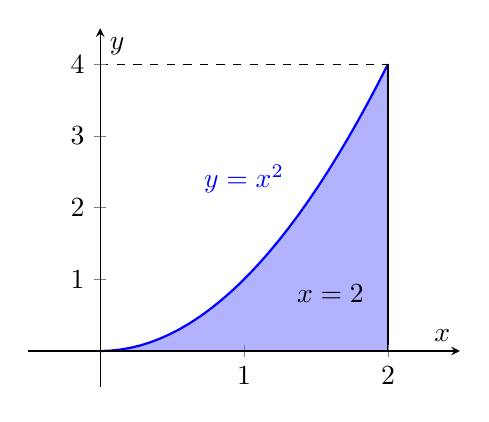
\begin{tikzpicture}
  \begin{axis}[
    axis lines=middle,
    xmin=-0.5, xmax=2.5,
    ymin=-0.5, ymax=4.5,
    xtick={0,1,2},
    ytick={0,1,2,3,4},
    xlabel=$x$, ylabel=$y$,
    domain=0:2,
    samples=30,
    axis on top,
    clip=true,
    scale=0.8,
    ]
    
    \addplot [
      draw=none,
      fill=blue!30,
    ]
    {x^2}
    \closedcycle;

    \addplot [thick, blue] {x^2};

    \draw (axis cs:2,0) -- (axis cs:2,4);
    \draw[dashed] (axis cs:0,4) -- (axis cs:2,4);
    \node[blue] at (1,2.4) {$y=x^2$};
    \node at (1.6,0.8) {$x=2$};
   \end{axis}
\end{tikzpicture}
\end{center}

\hfill

\noindent (a)
\begin{center}
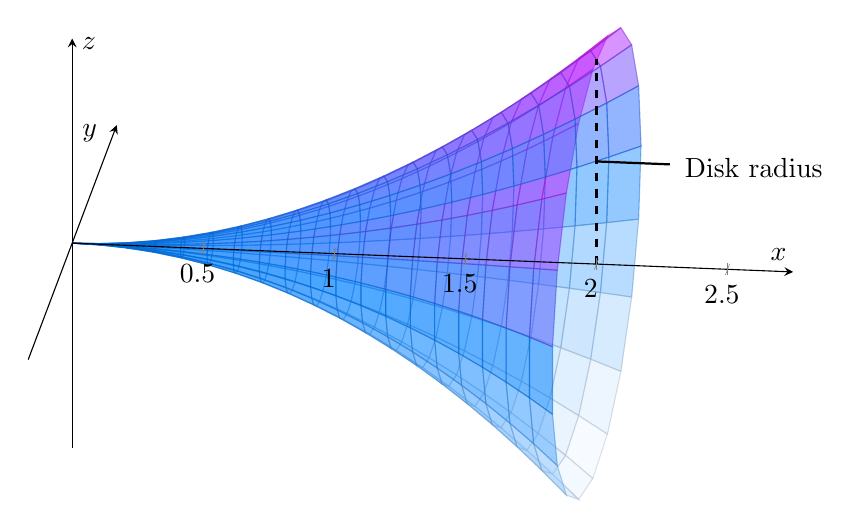
\begin{tikzpicture}
  \begin{axis}[
    view={7}{30},
    axis on top,
    axis lines=middle,
    xlabel={$x$},
    ylabel={$y$},
    zlabel={$z$},
    ytick={-4,4}, ztick={-4,4},
    samples=20,
    xmin=0, xmax=2.75,
    domain=0:2,
    y domain=0:360,
    colormap/cool,
    scale=1.5,
    ytick=\empty, ztick=\empty
    ]
    
    \addplot3 [
      surf,
      opacity=0.5,
    ]
    (
      x,
      {x^2 * cos(y)},
      {x^2 * sin(y)}
    );

    \draw[dashed, thick] (2,0,0)--(2,0,4);
    \draw[thick] (2,0,2)--(2.28,0,2);

    \node at (2.6,0,2) {Disk radius};
  \end{axis}
\end{tikzpicture}
\end{center}
\begin{align*}
\text{Volume}&=\int_{\mathcal{D}}\pi\cdot(r(x))^2\,dx=\int_0^2\pi\left(x^2\right)^2\,dx=\pi\int_0^2x^4\,dx=\pi\left[\frac{x^5}5\right]_0^2=\boxed{\frac{32\pi}5}
\end{align*}

\hfill

\noindent (b)
\begin{center}
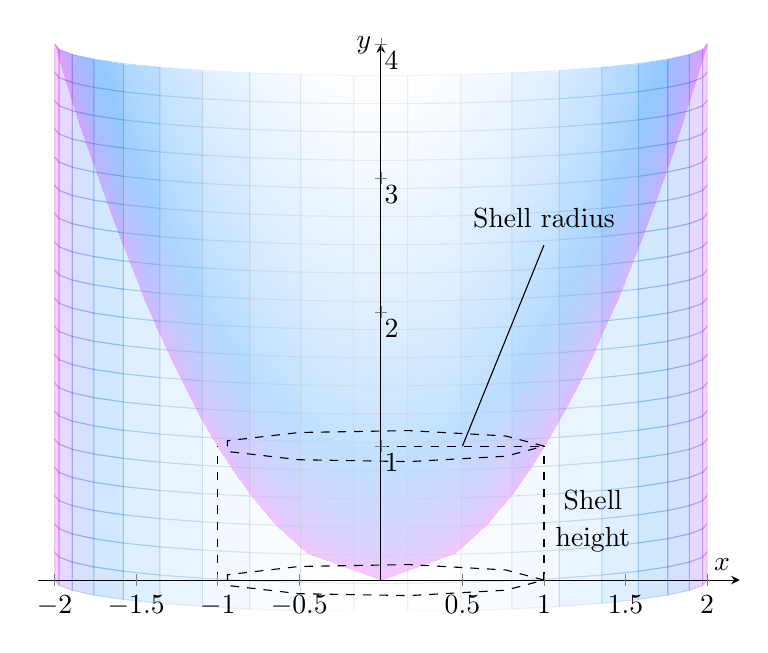
\begin{tikzpicture}
  \begin{axis}[
  view={0}{85},
    axis lines=center,
    axis on top,
    xlabel={$x$},
    ylabel={$y$},
    zlabel={$z$},
    hide z axis,
    xmin=-2.1, xmax=2.2,
    samples=20,
    domain=0:4,
    y domain=180:360,
    colormap/cool,
    scale=1.3,
    ]

    \addplot3 [
      surf,
      opacity=0.3,
      shader=interp,
    ]
    (
      {sqrt(x) * cos(y)},
      {x},
      {sqrt(x) * sin(y)}
    );
    
    \addplot3[
      surf,
      opacity=0.2,
    ]
    (
      {2 * cos(y)},
      {x},
      {2 * sin(y)}
    );

    \addplot3[
      domain=0:360,
      samples=10,
      dashed,
    ]
    (
      {cos(x)},
      {1},
      {sin(x)}
    );
    
    \addplot3[
      domain=0:360,
      samples=10,
      dashed,
    ]
    (
      {cos(x)},
      {0},
      {sin(x)}
    );
    \draw[dashed] (1,0,0)--(1,1,0);
    \draw[dashed] (-1,0,0)--(-1,1,0);
    \draw[dashed] (0,1,0)--(1,1,0);
    \draw (0.5,1,0)--(1,2.5,0);
    \node at (1.3,0.6,0) {Shell};
    \node at (1.3,0.3,0) {height};
    \node at (1,2.7,0) {Shell radius};
  \end{axis}
\end{tikzpicture}
\end{center}
\begin{align*}
\text{Volume}&=\int_{\mathcal{D}}2\pi\cdot r(x)\cdot h(x)\,dx=2\pi\int_0^2x\cdot x^2\,dx=2\pi\int_0^2x^3\,dx\\\\&=2\pi\left[\frac{x^4}4\right]_0^2=2\pi\left(\frac{2^4}4-0\right)=\boxed{8\pi}
\end{align*}

\noindent 2. 

\hfill

\noindent (a) The expression $\left|x^2-1\right|$ is the same as $x^2-1$ for $x>1$ and $1-x^2$ for $x<1$. We can write the equivalent expression below.

\begin{align*}\int_0^3\left|x^2-1\right|&=\,dx\int_0^1\left(1-x^2\right)\,dx+\int_1^3(x^2-1)\,dx=\left[x-\frac{x^3}3\right]_0^1+\left[\frac{x^3}3-x\right]_1^3\\\\&=\left[\left(1-\frac{1^3}3\right)-0\right]+\left[\left(\frac{3^3}3-3\right)-\left(\frac{1^3}3-1\right)\right]=\boxed{\frac{22}3}\end{align*}

\hfill

\noindent (b)
\begin{align*}\int\frac1{x^2+2x+1}\,dx=\int\frac1{(x+1)^2}\,dx=\boxed{-\frac1{x+1}+c, \quad c\in\mathbb{R}}\end{align*}

\hfill

\noindent (c)
\begin{align*}\int\frac1{x^2+2x+2}\,dx&=\int\frac1{(x+1)^2+1}\,dx\quad\left[u=x+1\implies du=dx\right]\\\\&=\int\frac1{u^2+1}\,du=\arctan(u)+c=\boxed{\arctan(x+1) +c,\quad c\in\mathbb{R}}\end{align*}

\hfill

\noindent (d) We can use the method of partial fraction decomposition.

\begin{equation}\int\frac1{x^2+3x+2}\,dx=\int\frac1{(x+1)(x+2)}\,dx=\int\left(\frac A{x+1}+\frac B{x+2}\right)\,dx\end{equation}

\begin{align*}
A(x+2)+B(x+1)&=1\\
x(A+B)+2A+B&=1\\
\therefore A+B=0\quad[\text{eliminate}\ x]\,&\rightarrow\,2A+B=1
\end{align*}

\[
\left.
\begin{array}{ll}
A+B=0\\
\displaystyle2A+B=1
\end{array}
\right\}
\quad A=1,\quad B=-1
\]

\hfill

\noindent Plug the values of $A$ and $B$ into $(1)$.

\begin{equation*}\int\left(\frac A{x+1}+\frac B{x+2}\right)\,dx=\int\left(\frac1{x+1}-\frac1{x+2}\right)\,dx=\boxed{\ln\left|x+1\right|-\ln\left|x+2\right|+c,\quad c\in\mathbb{R}}\end{equation*}

\hfill

\noindent (e) Use the trigonometric identity $\cos(2x)=1-2\sin^2x$.

\begin{equation*}\int_{-\pi/6}^0\sqrt{1-\cos(6x)}\,dx=\int_{-\pi/6}^0\sqrt{2\sin^2(3x)}\,dx=\sqrt2\int_{-\pi/6}^0\left|\sin(3x)\right|\,dx\end{equation*}

\hfill

\noindent $\sin x<0$ for $-\pi<x<\pi$. Therefore, the integral can be rewritten as follows.

\begin{align*}\sqrt2\int_{-\pi/6}^0\left|\sin(3x)\right|\,dx&=\sqrt2\int_{-\pi/6}^0-\sin(3x)\,dx=\sqrt2\left[\frac13\cos(3x)\right]_{-\pi/6}^0\\\\&=\frac{\sqrt2}3\left[\cos0-\cos\left(-\frac\pi2\right)\right]=\boxed{\frac{\sqrt2}3}\end{align*}

\hfill

\noindent 3. We have an improper integral where the limits are $\pm\infty$. Use limits to handle improper integrals accurately.

\begin{align*}
\int_{-\infty}^\infty\frac1{1+x^2}\,dx&=\lim_{A\to\infty}\int_{-A}^A\frac1{1+x^2}\,dx = \lim_{A\to\infty}\arctan(x)\bigg|_{-A}^A\\\\&=\lim_{A\to\infty}\left(\arctan A-\arctan(-A)\right)=\frac\pi2-\left(-\frac\pi2\right)=\boxed\pi
\end{align*}

\hfill

\noindent The value of the improper integral is finite. Therefore, this integral is convergent.

\hfill

\noindent 4.

\hfill

\noindent (a) The limit is in the indeterminate form $0/0$. We can apply L'Hôpital's rule to eliminate the indeterminate form.

\[\lim_{x\to0}\frac{3^x-1}{5^x-1}\overset{\text{L'H.}}{=}\lim_{x\to0}\frac{3^x\cdot\ln3}{5^x\cdot\ln5}=\log_53\cdot\lim_{x\to0}\left(\frac35\right)^x=\boxed{\log_53}\]

\hfill

\noindent (b) The first method is to evaluate the integral in the limit.

\[\lim_{x\to0}\frac{\displaystyle\int_0^{x^2}\sin t\,dt}x=\lim_{x\to0} \frac{-\cos t\,\bigg|_{t=0}^{t=x^2}}x=\lim_{x\to0}\frac{-\cos x^2-(-\cos0)}x=\lim_{x\to0}\frac{1-\cos x^2}x\]

\hfill

\noindent Multiply by the expression inside the limit $\displaystyle \frac xx$. Notice that we obtain a standard form.

\begin{align*}\lim_{x\to0}\left(\frac{1-\cos x^2}x\cdot\frac xx\right)&=\lim_{x\to0}\frac{1-\cos x^2}{x^2}\cdot\lim_{x\to0}x\quad\left[\lim_{u\to0}\frac{1-\cos u}u = 0\right]\\\\&=0\cdot0=\boxed0\end{align*}

\hfill

\noindent The second method is to use L'Hôpital's rule because of the $0/0$ form.

\[\lim_{x\to0}\frac{\displaystyle\int_0^{x^2}\sin t\,dt}x\overset{\text{L'H.}}{=}\lim_{x\to0}\frac{\displaystyle\frac d{dx}\int_0^{x^2}\sin t\,dt}1\]

\hfill

\noindent Let $u=x^2$, then $du=2x\,dx$. By the Fundamental Theorem of Calculus, the limit can be rewritten as follows.

\[\lim_{x\to0}\displaystyle\frac d{dx}\int_0^{x^2}\sin t\,dt=\lim_{x\to0}\frac d{du}\left(\int_0^u\sin t\,dt\right)\frac{du}{dx}=\lim_{x\to0}\left(\sin u\cdot 2x\right)=\lim_{x\to0}\left[2x\sin \left(x^2\right)\right]=\boxed0\]

\hfill

\noindent 5.

\hfill

\noindent (a)
\[a_n=\frac{2n+(-1)^n}{n}=2+\frac{(-1)^n}n\]

\hfill

\noindent The sequence converges to $\boxed2$ because $\displaystyle\frac{(-1)^n}n\to 0$ as $n\to\infty$.

\hfill

\noindent (b) $\arctan$ is continuous everywhere. Therefore, we can take the limit inside the expression.

\[\lim_{n\to\infty}\arctan\left(\frac{n+1}n\right)=\arctan\lim_{n\to\infty}\left(1+\frac1n\right)=\arctan1=\frac\pi4\]

\hfill

\noindent The sequence converges to $\displaystyle\boxed{\frac\pi4}$.

\hfill

\noindent (c)
\[\lim_{n\to\infty}\frac{n+1}{1-\sqrt n}=\lim_{n\to\infty}\frac{\sqrt n\left(\sqrt n+\frac1{\sqrt n}\right)}{\sqrt n\left(\frac1{\sqrt n}-1\right)}=\lim_{n\to\infty}\frac{\sqrt n+\frac1{\sqrt n}}{\frac1{\sqrt n}-1}=-\infty\]

\hfill

\noindent Notice that the denominator approaches $-1$ as $n\to\infty$ and the numerator approaches $\infty$ as $n\to\infty$. The sequence diverges to $\boxed{-\infty}$.

\newpage

\begin{center}
2011-2012 Fall Midterm I (15/11/2012) Solutions\\
(Last update: 12/10/2025 03:41)
\end{center}

\noindent 1.

\hfill

\noindent (a) Multiply each side by the conjugate of the denominator to eliminate the indetermination.

\begin{align*}
\lim_{x\to1}\frac{x^2+x-2}{\sqrt x -1}&=\lim_{x\to1}\left[\frac{(x+2)(x-1)}{\sqrt x -1}\cdot \frac{\sqrt x + 1}{\sqrt x +1}\right]=\lim_{x\to1}\frac{(x+2)(x-1)\left(\sqrt x + 1\right)}{x-1}\\\\&=\lim_{x\to1}\left[(x+2)\left(\sqrt x + 1\right)\right] =3\cdot 2 = \boxed6
\end{align*}

\hfill

\noindent (b)
\[\lim_{x\to 3}\frac{\sin(x^2-9)}{x-3}=\lim_{x\to 3}\left[\frac{\sin(x^2-9)}{x-3}\cdot\frac{x+3}{x+3}\right]=\lim_{x\to3}\left[\frac{\sin(x^2-9)}{x^2-9}\right]\cdot\lim_{x\to 3}(x+3)\]

\hfill

\noindent The value $\displaystyle \lim_{x\to0}\frac{\sin u}{u}$ can be evaluated by using the squeeze theorem, and it could be expected that we knew the value of this limit prior to the examination. Set $u=x^2-9$. So, the left-hand limit is $1$.

\[=\lim_{x\to3}\left[\frac{\sin(x^2-9)}{x^2-9}\right]\cdot\lim_{x\to 3}(x+3) = 1\cdot 6 = \boxed6\]

\hfill

\noindent (c) This is an indeterminate ($\infty - \infty$) form. We expand the expression by using its conjugate and dividing each side of the fraction by $x$ to eliminate the indeterminate form.

\begin{align*}&\lim_{x\to -\infty}\left(\sqrt{x^2-x+1}-\sqrt{x^2-2x}\right)\\\\&=\lim_{x\to -\infty}\left[\sqrt{x^2-x+1}-\sqrt{x^2-2x}\cdot\frac{\sqrt{x^2-x+1}+\sqrt{x^2-2x}}{\sqrt{x^2-x+1}+\sqrt{x^2-2x}}\right]\\\\&=\lim_{x\to-\infty}\frac{x^2-x+1-\left(x^2-2x\right)}{\sqrt{x^2-x+1}+\sqrt{x^2-2x}}=\lim_{x\to-\infty}\left(\frac{x+1}{\sqrt{x^2-x+1}+\sqrt{x^2-2x}}\cdot\frac{x}{x}\right)\\\\&=\lim_{x\to-\infty}\frac{\displaystyle\frac{x+1}x}{\displaystyle\frac{|x|\sqrt{1-\frac1x+\frac1{x^2}}+|x|\sqrt{1-\frac1x}}x}=\lim_{x\to-\infty}-\frac{\displaystyle1+\frac{1}x}{\displaystyle\sqrt{1-\frac1x+\frac1{x^2}}+\sqrt{1-\frac2x}}\quad\Big[|x|=-x\Big]\\\\&=-\frac{1-0}{\sqrt{1+0-0}+\sqrt{1+0}}=\boxed{-\frac12}\end{align*}

\newpage

\noindent 2.

\hfill

\noindent (a) Apply the chain rule accordingly.
\[\boxed{f'(x) = 3\tan^2\left(4\sin^2(3x)\right)\cdot \sec^2\left(4\sin^2(3x)\right)\cdot8\sin(3x)\cdot \cos(3x)\cdot 3}\]

\hfill

\noindent (b) Take the logarithm of both sides to differentiate easily.
\[\ln\left(f(x)\right)=\ln\left[\left(\cos x^2\right)^x\right]=x\ln\left(\cos x^2\right)\]

\[\frac{d}{dx}\,\ln\left(f(x)\right)=\frac{d}{dx}\left[x\ln\left(\cos x^2\right)\right]\]

\[\frac1{f(x)}\cdot f'(x)=1\cdot\left[\ln\left(\cos x^2\right)\right]+x\cdot\frac1{\cos x^2}\cdot\left(-\sin x^2\right)\cdot2x\]

\[f'(x)=f(x)\left[\ln\left(\cos x^2\right)-2x^2\cdot\tan x^2\right]\]

\[\boxed{f'(x)=\left(\cos x^2\right)^x\cdot\left[\ln\left(\cos x^2\right)-2x^2\cdot\tan x^2\right]}\]

\hfill

\noindent (c) Rewrite the right-hand side using the property of logarithms. Take the first derivative afterwards.

\[f(x)=\ln\left(\frac{3^x}{3^x+1}\right)=\ln\left(3^x\right)-\ln\left(3^x+1\right)\]

\[f'(x)=\frac1{3^x}\cdot 3^x\cdot\ln(3)-\frac1{3^x+1}\cdot3^x\cdot\ln(3)=\ln(3)\cdot\left[1-\frac{3^x}{3^x+1}\right]\]

\[f'(0)=\ln(3)\cdot\left[1-\frac{3^0}{3^0+1}\right]=\boxed{\frac{\ln3}2}\]

\hfill

\noindent 3. Let $L$ be the value of the limit.

\[L = \lim_{x\to0}\left(\mathrm{e}^x-x\right)^{\frac1x}\]
\[\ln(L) = \ln\left[\lim_{x\to0}\left(\mathrm{e}^x-x\right)^{\frac1x}\right]\]

\hfill

\noindent The expression is defined for $x\neq0$. Therefore, we can take the logarithm function inside the limit. After that, apply L'Hôpital's rule to eliminate the indeterminate form.

\begin{align*}\ln(L)&=\lim_{x\to0}\ln\left[\left(\mathrm{e}^x-x\right)^{\frac1x}\right]=\lim_{x\to0}\frac{\ln\left(\mathrm{e}^x-x\right)}x\quad\left[\frac00\right]\\\\&\overset{\text{L'H.}}{=}\lim_{x\to0}\frac{\displaystyle\frac{1}{\mathrm{e}^x-x}\cdot\left(\mathrm{e}^x-1\right)}{1}=\lim_{x\to0}\frac{\mathrm{e}^x-1}{\mathrm{e}^x-x}=\frac{\mathrm{e}^0-1}{\mathrm{e}^0-0}=0\end{align*}

\hfill

\noindent If $\ln(L)=0$, then $\boxed{L=1}$.

\newpage

\noindent 4.

\hfill

\noindent (a) \[p(x)=1-2F\left(\frac x3\right)\]
\[p(x)-1=-2F\left(\frac x3\right)\]
\[\frac{1-p(x)}{2}=F\left(\frac x3\right)\]
\[F^{-1}\left(\frac{1-p(x)}{2}\right)=\frac x3\]
\[3F^{-1}\left(\frac{1-p(x)}{2}\right)=x\]
\[3F^{-1}\left(\frac{1-p\left(p^{-1}(x)\right)}{2}\right)=p^{-1}(x)\]

\[\boxed{p^{-1}(x)=3F^{-1}\left(\frac{1-x}{2}\right)}\]

\hfill

\noindent (b) Find a root so that $f(x_0) = \arctan(x_0)+\mathrm{e}^{123\cdot x_0} = 1$. We can intuitively say that the root is small because both $\arctan x$ and $\mathrm{e}^x$ are strictly increasing everywhere. Try $x=0$.

\[f(0)=\arctan 0+\mathrm{e}^{123\cdot 0}=0+1=1\]

\hfill

\noindent Therefore, $f^{-1}(1)=0$. The derivative of an inverse function at a given point is

\[\left(f^{-1}\right)'(1)=\frac1{f'(f^{-1}(1))}\]

\hfill

\noindent Calculate $f'(x)$ and $(f^{-1})(1)$.

\[f'(x)=\frac1{1+x^2}+123\mathrm{e}^{122x}\]

\[\left(f^{-1}\right)'(1)=\frac{1}{f'(0)}=\left( \frac1{1+0^2}+123\mathrm{e}^{122\cdot0} \right)^{-1}=\boxed{\frac1{124}}\]

\hfill

\noindent 5. Consider $y=f(x)$. Differentiate both sides implicitly.

\[\frac{d}{dx}\left(x^2y^2-36x\right) = \frac{d}{dx}\,37\]

\[2xy^2+ x^2\cdot2y\cdot \frac{dy}{dx}-36 = 0\]

\[x^2\cdot2y\cdot \frac{dy}{dx}=36 - 2xy^2\]

\[\frac{dy}{dx}=\frac{36-2xy^2}{x^2\cdot2y}\]

\hfill

\noindent Calculate $\displaystyle \frac{dy}{dx}$ at $(-1,1)$.

\hfill

\begin{equation}\frac{dy}{dx}\Bigg|_{(-1,1)}=\frac{36-2(-1)\cdot1^2}{(-1)^2\cdot2\cdot1} = 19\end{equation}

\hfill

\noindent Using the straight line formula, we find the tangent line. Recall: $y-y_0=m(x-x_0)$, where $m$ can be substituted with $(1)$.

\[\boxed{y-1=19(x+1)}\]

\hfill

\noindent 6. Let $x(t),\,y(t),\,l(t)$ represent the lengths of the sides as functions of time. We can set up the following equation for the area of the right triangle.

\[A(t) = \frac{x(t)\cdot y(t)}{2}\]

\hfill

\noindent Take the derivative of both sides.

\begin{equation}A'(t) =\frac12\left(x'(t)\cdot y(t) + x(t)\cdot y'(t) \right)\end{equation}

\hfill

\noindent We also know that, by the Pythagorean theorem,

\[l^2(t) = x^2(t)+y^2(t)\]

\hfill

\noindent Take the derivative of both sides.

\[2l(t)l'(t)= 2x(t)x'(t)+2y(t)y'(t)\]

\hfill

\noindent Since the length of the hypotenuse is constant, $l'(t) = 0$. Therefore,

\begin{equation}x(t)x'(t)=-y(t)y'(t)\end{equation}

\hfill

\noindent At $t=t_0$, we have $l(t_0) = 5,\,x(t_0)=3,\,x'(t_0)=-2$, and by the Pythagorean theorem, $y(t_0)=\sqrt{5^2-3^2}=4$. Calculate $y'(t_0)$ from $(3)$.

\[y'(t_0)=-\frac{3\cdot (-2)}4 = \frac32\]

\hfill

\noindent Plug the necessary values into $(2)$ to find the rate of change of the area.

\[A'(t_0) =\frac12\left((-2)\cdot4+3\cdot\frac32\right)=\boxed{-\frac74\,\text{cm}^2/\text{s}}\]

\newpage

\begin{center}
2012-2013 Fall Midterm II (19/12/2012) Solutions\\
(Last update: 29/08/2025 19:47)
\end{center}

\noindent 1. Let $x$ be the length of the wire that is used to form the equilateral triangle. So, $10-x$ is the length of the other piece. The area of the triangle is

\begin{equation*}
A_1 = \frac{x^2\sqrt3}{4}
\end{equation*}

\hfill

\noindent The perimeter of the circle is $10-x$. Therefore, $2\pi r = 10-x$, where $r$ is the radius of the circle. The area of the circle can be extracted from the formula $A_2=\pi r^2$. Solve the former equation for $r$, and express the area in terms of $x$.

\begin{equation*}
    r=\frac{10-x}{2\pi}\,\rightarrow\, A_2 = \pi\left(\frac{10-x}{2\pi}\right)^2 =\frac{100-20x+x^2}{4\pi}
\end{equation*}

\hfill

\noindent Let $A(x)$ be the function of length representing the sum of the areas.

\begin{equation*}
    A(x) = \frac{x^2\sqrt3}{4}+\frac{100-20x+x^2}{4\pi}
\end{equation*}

\hfill

\noindent Minimize $A(x)$ by taking the first derivative and setting it to $0$.

\begin{equation*}
A'(x)=\frac{x\sqrt3}{2} + \frac{x-10}{2\pi}=0\,\rightarrow\,10=x+x\cdot\pi\sqrt3\,\rightarrow\,x=\frac{10}{1+\pi\sqrt3}
\end{equation*}

\hfill

\noindent The length of the piece used to form the triangle is $\displaystyle\frac{10}{1+\pi\sqrt3}$, the length of the other piece is $\displaystyle\frac{10\pi\sqrt3}{1+\pi\sqrt3}$.

\hfill

\noindent 2.

\hfill

\noindent (a) Let $u=1+\sqrt y$, then $\displaystyle du=\frac{dy}{2\sqrt y}$.

\begin{equation*}
\int\frac{dy}{\sqrt{y}\left(1+\sqrt y\right)^2}=\int\frac{1}{u^2}\cdot2\,du=-\frac{2}{u}+c=\boxed{-\frac{2}{1+\sqrt y}+c,\,c\in\mathbb{R}}
\end{equation*}

\hfill

\noindent (b) Let $u=\ln(\sin x)$, then $\displaystyle du=\frac{1}{\sin x}\cdot \cos x\,dx$.

\begin{align*}
\int_{\pi/6}^{\pi/4}\frac{\cot x}{\ln(\sin x)}\,dx&=\int\frac1u\,du=\ln|u| + c=\Big[\ln\left|\ln(\sin x)\right| \Big]_{\pi/6}^{\pi/4}\\\\&=\ln\left|\ln\frac{\sqrt2}2\right|-\ln\left|\ln\frac12\right|=\ln\frac{\left|\ln\frac{\sqrt2}{2}\right|}{\left|\ln\frac12\right|}\\\\&=\ln\left(\frac{\ln2-\ln\sqrt2}{\ln2-\ln1}\right)=\ln\frac12=\boxed{-\ln2}
\end{align*}

\hfill

\noindent (c) Attempt a long polynomial division and split into two integrals.

\begin{align*}
\mathrm{I}=\int\frac{x^3-4x-10}{x^2-x-6}\,dx&=\int(x+1)\,dx+\int\frac{3x-4}{(x-3)(x+2)}\,dx\\\\&=\frac{x^2}2+x+\int\left({\frac{A}{x-3}+\frac{B}{x+2}}\right)\,dx
\end{align*}

\begin{align*}
A(x+2)+B(x-3)&=3x-4\\
x(A+B)+2A-3B&=3x-4\\
\end{align*}
\[
\left.
\begin{array}{ll}
A+B=3\\
2A-3B=-4
\end{array}
\right\}
\quad A=1,\quad B=2
\]

\begin{equation*}
\mathrm{I}=\frac{x^2}2+x+\int\left({\frac{1}{x-3}+\frac{2}{x+2}}\right)\,dx=\boxed{\frac{x^2}2+x+\ln|x-3|+2\ln|x+2|+c,\,c\in\mathbb{R}}
\end{equation*}

\hfill

\noindent (d) Let $u=\sec x$, then $du=\tan x \sec x \,dx$.

\begin{align*}\int\tan x\sec^{123}x\,dx=\int u^{122}\,du=\frac{u^{123}}{123}+c = \boxed{\frac{\sec^{123}x}{123}+c,\,c\in\mathbb{R}}\end{align*}

\hfill

\noindent (e) Let $t=\sin^2x$, then $dt=2\sin x\cos x\,dx$.

\begin{align*}\int\sqrt{t-t^2}\,dt&=\int\sqrt{\sin^2x-\sin^4x}\cdot2\sin x \cos x \,dx=\int\sqrt{\sin^2x\cdot(1-\sin^2x)}\cdot\sin(2x)\,dx\\\\&=\int\sin x \cos x\cdot\sin(2x)\,dx=\frac12\int\sin^2(2x)\,dx=\frac12\int\left(1-\cos^2(2x)\right)\,dx\\\\&=\frac12\int\frac{1-\cos(4x)}2\,dx=\frac14\left[x-\frac14\sin(4x)\right]+c,\,c\in\mathbb{R}\end{align*}

\hfill

\noindent We will try to rewrite the result in terms of $t$.

\[t-t^2 \geq 0\implies 0\leq t \leq 1\]
\[t=\sin^2x \implies\sqrt t = \sin x\implies\arcsin\left(\sqrt t\right) = x\]
\[t=\sin^2x=1-\cos^2x\implies \cos x= \sqrt{1-t}\]
\[\sin(4x)=2\sin(2x)\cos(2x)=4\sin x\cos x\left(2\cos^2x-1\right)=4\sqrt t\cdot\sqrt{1-t}\cdot(1-2t)\]

\begin{align*}
\int\sqrt{t-t^2}\,dt=\boxed{\frac14\left[\arcsin\left(\sqrt t\right)-\sqrt{t(1-t)}\cdot(1-2t)\right]+c,\,c\in\mathbb{R}}
\end{align*}

\hfill

\noindent (f) Let $u=\sqrt{1+\sqrt x}$.

\[u^2 = 1+\sqrt x\implies u^2-1 = \sqrt x\implies\left(u^2-1\right)^2 = x\implies2\left(u^2-1\right)\cdot 2u\,du = dx\]

\begin{align*}
\int \sqrt{1+\sqrt{x}}\,dx&=\int u \cdot(2u^2-2)\cdot 2u\,du=\int\left(4u^4-4u^2\right)\,du=\frac{4u^5}5-\frac{4u^3}{3} + c\\\\&=\boxed{\frac{4\left(\sqrt{1+\sqrt x}\right)^5}5-\frac{4\left(\sqrt{1+\sqrt x}\right)^3}3+c,\,c\in\mathbb{R}}\end{align*}

\hfill

\noindent 3.

\hfill

\noindent (a)
\begin{align*}
\int_0^2\frac{dx}{\sqrt{|x-1|}}&=\int_0^1\frac{dx}{\sqrt{1-x}} + \int_1^2\frac{dx}{\sqrt{x-1}}=\lim_{S\to1^-}\int_0^S\frac{dx}{\sqrt{1-x}}+\lim_{P\to1^+}\int_P^2\frac{dx}{\sqrt{x-1}}\\\\&=\lim_{S\to1^-}\left[-2\sqrt{1-x}\right]_0^S+\lim_{P\to1^+}\left[2\sqrt{x-1}\right]_P^2\\\\&=\lim_{S\to1^-}\left[-2\sqrt{1-S}\right]+2\sqrt{1-0}+2\sqrt{2-1}-\lim_{P\to1^+}\left[2\sqrt{P-1}\right]=\boxed4
\end{align*}

\hfill

\noindent (b)
\begin{align*}\int_{-\infty}^{\infty} x^2\mathrm{e}^{-x^{3}}\,dx=\lim_{a\to\infty}\int_{-a}^{a} x^2\mathrm{e}^{-x^{3}}\,dx=\lim_{a\to\infty}-\frac13\left[\mathrm{e}^{-x^3}\right]_{-a}^a=\lim_{a\to\infty}-\frac13\left[\mathrm{e}^{-a^3}-\mathrm{e}^{a^3}\right]=\boxed\infty\end{align*}

\hfill

\noindent 4.

\begin{minipage}{0.45\textwidth}
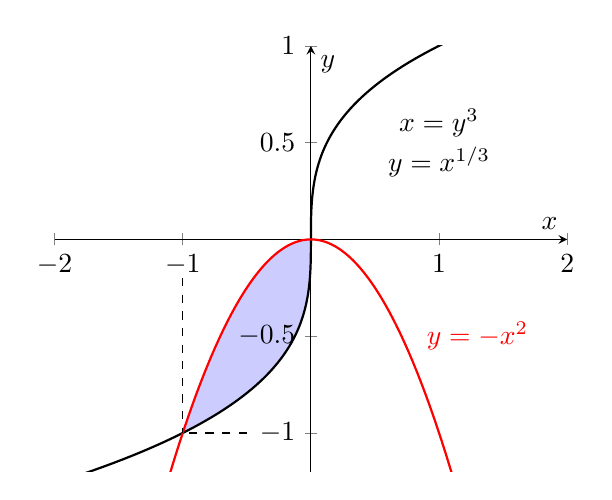
\begin{tikzpicture}
  \begin{axis}[
    axis lines = middle,
    xlabel = {$x$},
    ylabel = {$y$},
    ymin = -1.2, ymax = 1,
    xmin = -2, xmax = 2,
    samples = 200,
    domain = -2:2,
    clip=true,
    scale=0.95,
  ]

  \addplot [
    name path=A,
    domain=-1:0,
    draw=none,
  ] {-x^2};

  \addplot [
    name path=B,
    domain=-1:0,
    draw=none,
  ] ({x^3}, x);

  \addplot [
    fill=blue!20,
  ] fill between[of=A and B];

  \addplot [
    domain=-2:2,
    samples=200,
    thick,
    black,
  ] ({x^3}, x);

  \addplot [
    domain=-2:2,
    samples=200,
    thick,
    red,
  ] {-x^2};

  \draw[dashed] (axis cs:-1,-0.2) -- (axis cs:-1,-1);
  \draw[dashed] (axis cs:-0.5,-1) -- (axis cs:-1,-1);

  \node[red] at (axis cs: 1.3,-0.5) {$y=-x^2$};
  \node at (axis cs: 1,0.6) {$x=y^3$};
  \node at (axis cs: 1,0.4) {$y=x^{1/3}$};

  \end{axis}
\end{tikzpicture}
\end{minipage}
\begin{minipage}{0.5\textwidth}
\begin{align*}
V&=\int_{-1}^0\pi\left[\left(x^{1/3}\right)^2-\left(-x^2\right)^2\right]\,dx\\\\&=\pi\int_{-1}^0\left(x^{2/3}-x^4\right)\,dx\\\\&=\pi\left[\frac35x^{5/3}-\frac{x^5}{5}\right]_{-1}^0\\\\&=\pi\cdot\left[0-\left(-\frac35+\frac15\right)\right]=\boxed{\frac{2\pi}5}
\end{align*}\
\end{minipage}

\newpage

\begin{center}
2015-2016 Fall Midterm (10/12/2015) Solutions\\
(Last update: 29/08/2025 20:34)
\end{center}

\noindent 1. Take the first derivative and set to 0.

\[f'(x)=-\frac{1}{x^2}-\frac{2}{x^3}\]
\[f'(x)=0\implies \frac{2}{x^3} = -\frac{1}{x^2}\implies x = -2 \quad(\text{candidate for a critical point})\]

\hfill

\noindent Take the second derivative and set to 0.

\[f''(x)=\frac{2}{x^3}+\frac{6}{x^4}\]
\[f''(x)=0\implies\frac{1}{x^3}=-\frac{3}{x^4}\implies x=-3\quad(\text{candidate for an inflection point})\]

\hfill

\noindent $\{-2,-3\}\subset\mathcal D$. Therefore, $f(-2)$ gives rise to a local extremum. The sign of the first derivative changes from minus to plus, meaning $f(-2)$ is a local minimum. $x=-3$ gives rise to an inflection point because the sign of the second derivative also changes.

\hfill

\noindent Find the asymptotes.

\[\lim_{x\to\infty}f(x)=\lim_{x\to-\infty}f(x)=0\]

\hfill

\noindent $y=0$ is the horizontal asymptote and $x=0$ is the vertical asymptote.

\hfill

\noindent Let us find monotonicity and concavity. If the sign of $f'(x)$ is minus, the function is decreasing on the corresponding interval; otherwise, increasing. If the sign of $f''(x)$ is minus, the graph of the function is concave downward; otherwise, concave upward.

\begin{center}
    \large
    \begin{tabular}{ |c| c c c c| } 
    \hline
        $x$ & $(-\infty, -3)$ & $(-3, -2)$ & $(-2, 0)$ &  $(0, \infty)$ \\
        \hline
        $f'$ sign & - & - & + & - \\
        \hline
        $f''$ sign & - & + & + & + \\
        \hline
    \end{tabular}
\end{center}

\hfill

\noindent Eventually, sketch the graph.

\begin{center}
\begin{tikzpicture}
  \begin{axis}[
    axis lines = center,
    xlabel = $x$,
    ylabel = $y$,
    domain=-3:-0.1,
    samples=200,
    ymin=-0.3, ymax=10,
    xmin=-5, xmax=5,
    restrict y to domain=-1:8,
    restrict x to domain=-5:5,
    legend pos=outer north east,
    clip=true,
    scale=1.2
  ]
  
  \node[blue] at (3,6) {$f(x) = \dfrac{1}{x} + \dfrac{1}{x^2}$};
  \addplot[blue, thick, domain=-5:-0.1] {1/x + 1/(x^2)};
  \addplot[blue, thick, domain=0.1:4.4] {1/x + 1/(x^2)};
  
  \draw[dashed, red] (axis cs:-5,0.05) -- (axis cs:5,0.05);
  \draw[dashed, red] (axis cs:0.05,-30) -- (axis cs:0.05,30);
  \end{axis}
\end{tikzpicture}
\end{center}

\hfill

\noindent 2. Let $f(x) = 3\tan x + x^3 -2$. $f$ is continuous on $[0, \pi/4]$ and differentiable on $(0, \pi/4)$. By IVT (Intermediate Value Theorem), there exists at least one point where $f(x) = 0$ because $f(0) = -2$ and $f(\pi/4) = 1 + (\pi/4)^3$. Assume that we have two roots on the interval, so at some point c, $f'(c) = 0$.

\[f'(x) = 3\sec^2x + 3x^2\implies  f'(c) = 3\sec^2c + 3c^2 = 0\implies \sec^2c =-c^2 \]

\hfill

\noindent Since $-c^2 \leq 0$ and $\sec ^2c > 0$, there is no $c$ that satisfies the equation. This contradicts our assumption that we have two roots on the interval. By Rolle's theorem, there is only one root on the interval $[0, \pi/4]$.

\hfill

\noindent 3. Implicitly differentiate both sides.

\[\frac{d}{dx}\left[x \sin\left(xy-y^2\right)\right] = \frac{d}{dx}\left(x^2-1\right) \]

\[1\cdot\sin\left(xy-y^2\right)+x\cdot\cos\left(xy-y^2\right)\cdot\left[\left(1\cdot y+x\frac{dy}{dx}\right)-2y\frac{dy}{dx}\right]=2x\]

\hfill

\noindent Rearrange the equation to solve for $\frac{dy}{dx}$ through a careful and rigorous attempt.

\[x\cdot\cos\left(xy-y^2\right)\cdot\left[\left(1\cdot y+x\frac{dy}{dx}\right)-2y\frac{dy}{dx}\right]=2x-\sin(xy-y^2)\]

\[y+\frac{dy}{dx}(x-2y)=\frac{2x-\sin\left(xy-y^2\right)}{x\cdot\cos\left(xy-y^2\right)}\]

\[\frac{dy}{dx}(x-2y)=\frac{2x-\sin\left(xy-y^2\right)}{x\cdot\cos\left(xy-y^2\right)}-y\]

\hfill

\begin{equation}\frac{dy}{dx}=\frac{\frac{2x-\sin(xy-y^2)}{x\cdot\cos(xy-y^2)}-y}{(x-2y)}\end{equation}

\hfill

\noindent Calculate $\left.\dfrac{dy}{dx}\right|_{(1,1)}$ from $(1)$. This will give us the slope of the tangent line.

\[\left.\frac{dy}{dx}\right|_{(1,1)}=-1\]

\hfill

\noindent Recall: $y-y_0 = m(x-x_0)$. $m$ is $\dfrac{dy}{dx}$ at $x=1$. So, the tangent line is:

\[y-1=-(x-1)\implies\boxed{y=2-x}\]

\hfill

\noindent 4.

\hfill

\noindent (a) Let L be the value of the limit. Then, take the logarithm of both sides.

\[L = \lim_{x\to 0^+} (1+\sin x)^{\frac{1}{x}}\]

\[\ln(L)=\ln\left[\lim_{x\to 0^+} (1+\sin x)^{\frac{1}{x}}\right]\]

\hfill

\noindent The expression on the right is continuous for $x>0$. Therefore, we can take the logarithm inside the limit.

\[\ln(L)=\lim_{x\to 0^+}\ln\left[(1+\sin x)^{\frac{1}{x}}\right]=\lim_{x\to 0^+}\left[\frac{\ln(1+\sin x)}{x}\right]\]

\hfill

\noindent If we substitute $x=0$, the limit is in the form $0/0$. L'Hôpital's rule states that we may take the derivatives of both sides of the fraction if there's a $0/0$ indeterminate form. Apply the chain rule accordingly.

\[\lim_{x\to 0^+} \left[\frac{\ln(1+\sin x)}{x}\right]\overset{\text{L'H.}}{=}\lim_{x\to 0^+} \left[\frac{\frac{1}{1+\sin x}\cdot\cos x}{1}\right]=\lim_{x\to 0^+}\left[\frac{\cos x}{1+\sin x}\right] \]

\hfill

\noindent The limit can now be evaluated by substituting $x=0$.

\[\lim_{x\to 0^+} \left[\frac{\cos x}{1+\sin x}\right] = \frac{\cos 0}{1 + \sin 0 } =1\]

\hfill

\noindent Now, $\ln(L) = 1$. Simply, take $L$ out of the logarithm.

\[ \boxed{L = \mathrm{e}}\]

\hfill

\noindent (b) Look at the one-sided limits. Let us first evaluate the limit from the right side. Above and near $x=3$, the floor function will return $9$.

\[ \lim_{x\to 3^+} \frac{x^2-\floor{x^2}}{x-3} = \lim_{x\to 3^+}\frac{x^2-9}{x-3} = \lim_{x\to 3^+}\frac{(x-3)(x+3)}{x-3} = \lim_{x\to 3^+}(x+3)= 6\]

\hfill

\noindent From the left side, the output is the largest integer less than $9$. Therefore, $\floor{x^2} = 8$.

\[ \lim_{x\to 3^-} \frac{x^2-\floor{x^2}}{x-3} = \lim_{x\to 3^-}\frac{x^2-8}{x-3} = -\infty\]

\hfill

\noindent The one-sided limits are not equal to each other. Therefore, the limit does not exist.

\hfill

\noindent 5. $x=x(t)$ and $y=y(t)$. The distance between the point P and the origin, and the distance between the point P and the point (7,0) are, respectively, given by:

\[f(t) = \sqrt{(x-0)^2 + (y-0)^2} = \sqrt{x^2+y^2}\]

\[g(t) = \sqrt{(x-7)^2 + (y-0)^2} = \sqrt{x^2-14x +49+y^2}\]

\hfill

\noindent Take the first derivative with respect to time.

\begin{equation}f'(t)=\frac{1}{2\sqrt{x^2+y^2}}\cdot\left(2x\frac{dx}{dt}+2y\frac{dy}{dt}\right)\end{equation}

\begin{equation}g'(t)=\frac{1}{2\sqrt{x^2-14x +49+y^2}}\cdot\left((2x-14)\frac{dx}{dt}+2y\frac{dy}{dt}\right)\end{equation}

\hfill

\noindent For $t=t_0$, it is given $x(t_0) = 4,\,y(t_0) = 3$ and $f(t_0) = \sqrt{4^2 +3^2} = 5,\,g(t_0) = \sqrt{3^2 + 3^2} = 3\sqrt{2}$. We then obtain a system of two equations by substituting values in (2) and (3):

\[f'(t_0)=\frac{1}{10}\cdot\left(8\frac{dx}{dt}+6\frac{dy}{dt}\right)=\sqrt{2}\]

\[g'(t_0)=\frac{1}{6\sqrt{2}}\cdot\left((-6)\frac{dx}{dt}+6\frac{dy}{dt}\right)=-3\]

\hfill

\noindent Let us simplify the equations.

\[4x'(t_0)+3y'(t_0) = 5\sqrt{2} \]
\[-3x'(t_0)+3y'(t_0) = -9\sqrt{2} \]

\hfill

\noindent The question asks us to find the change in the $x$-coordinate of P. Therefore, negate the latter equation and solve for $x'(t_0)$.

\[ \boxed{x'(t_0) = 2\sqrt{2}} \]

\hfill

\noindent 6.

\begin{center}
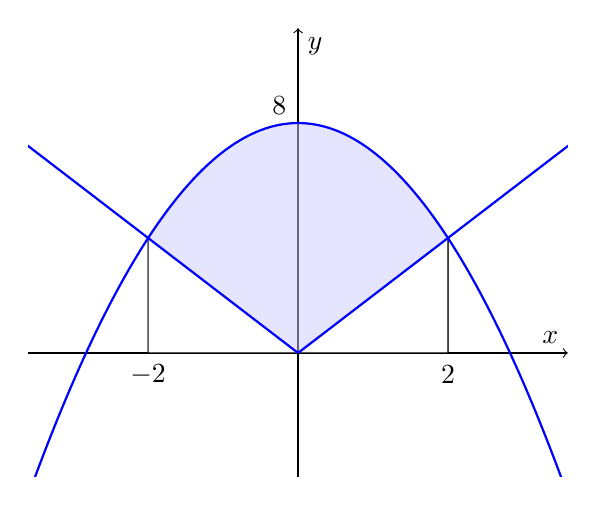
\begin{tikzpicture}
  \begin{axis}[
    axis lines = center,
    xlabel = $x$, ylabel = $y$,
    domain=-4:4,
    samples=300,
    ymin=-3, ymax=10,
    xmin=-3, xmax=3,
    restrict y to domain=-10:10,
    enlargelimits=true,
    legend pos=outer north east,
    axis line style={->},
    xtick=\empty, ytick=\empty
    ]
    \addplot [
      domain=-2:2,
      samples=200,
      fill=blue!20,
      opacity=0.5
    ]
    {8 - x^2} \closedcycle;

    \addplot [
      domain=-2:2,
      samples=200,
      fill=white,
    ]
    {2*abs(x)} \closedcycle;
    
    \addplot[blue, thick] {2*abs(x)};
    \addplot[blue, thick] {8-x^2};

    \node at (-2,-0.75) {$-2$}; \node at (2,-0.75) {$2$};
    \node at (-0.25,8.6) {$8$};

  \end{axis}
\end{tikzpicture}
\end{center}

\noindent The area can be found by integrating the difference in $y$ with respect to $x$. We split the integral into two because the absolute value function changes sign.

\[\mathrm{I}=\int_{-2}^2(8-x^2-2|x|)\,dx=\int_{-2}^0(8-x^2+2x)\,dx+\int_{0}^2(8-x^2-2x)\,dx\]

\[\mathrm{I}=\left[8x-\frac{x^3}{3}+x^2\right]_{-2}^0+\left[8x-\frac{x^3}{3}-x^2\right]_{0}^2\]

\[\mathrm{I}=0-\left({-16}+\frac{8}{3}+4\right)+\left(16-\frac{8}{3}-4\right)-0=\boxed{\frac{56}{3}}\]

\newpage

\begin{center}
2016-2017 Fall Midterm (05.12.2016) Solutions\\
(Last update: 29/08/2025 20:46)
\end{center}

\noindent 1.

\hfill

\noindent (a) To solve the limit easily, we can use logarithms. The expression is continuous and differentiable for $x > 0$. Assume that the limit exists, then let L be the value of the limit.

\[ L = \lim_{x \to \infty} [\mathrm{e}^x + 1]^{\frac{1}{x}} \]

\[
\ln(L) = \ln\left(\lim_{x \to \infty} [\mathrm{e}^x + 1]^{\frac{1}{x}}\right) = \lim_{x \to \infty} \left[ \ln\left( [\mathrm{e}^x + 1]^{\frac{1}{x}} \right) \right]
\]

\[
\ln(L) = \lim_{x \to \infty} \left[ \frac{\ln(\mathrm{e}^x + 1)}{x}\right]
\]

\hfill

\noindent The expressions $x$ and $\mathrm{e}^x + 1$ tend to infinity as $x$ approaches infinity. L'Hôpital's rule suggests that we take the derivatives of both sides of the fraction if there's an indeterminate form of infinity ($\frac{\infty}{\infty}$). Using the chain rule, we get:

\[\ln(L) \overset{\text{L'H.}}{=} \lim_{x \to \infty} \left[ \frac{\frac{1}{\mathrm{e}^x+1} \cdot \mathrm{e}^x}{1}\right] = \lim_{x \to \infty} \left( \frac{\mathrm{e}^x}{\mathrm{e}^x+1} \right)\]

\hfill

\noindent It is obvious that $\ln(L) = 1$. $\mathrm{e}^x$ grows at the same rate as $\mathrm{e}^x + 1$. The behavior can be confirmed using L'Hôpital's rule. Without further ado, we can convert the logarithm back to its original form.

\[\ln(L) = 1\]
\[\boxed{L = \mathrm{e}}\]

\hfill

\noindent (b) If we substitute for $x = 1$, it is in the form $0/0$. Multiply each side by the conjugate of the denominator.

\[
\lim_{x \to 1}\left( \frac{x-1}{\sqrt{x+3} - 2} \cdot \frac{\sqrt{x+3} + 2}{\sqrt{x+3} + 2} \right) = \lim_{x \to 1} \frac{(x-1)(\sqrt{x+3} + 2)}{x-1} = \lim_{x \to 1} (\sqrt{x+3} + 2) = \boxed 4\]

\hfill

\noindent 2. If $f$ is continuous at a point, then the one-sided limits must be equal to the value of the function at that point. $f$ is constant for $x < 2$, meanwhile polynomial for $x \geq 2$. If we check the point where $x=2$, the continuity will be provided for all $x$.

\[\lim_{x\to2^-}f(x)=12,\quad\lim_{x\to2^+}f(x)=a^2x-2a\implies12=2a^2-2a\]

\[2(a^2-a-6)=0\implies(a-3)(a+2)=0\implies\boxed{a_1=3,\:a_2=-2}\]

\hfill

\noindent 3. Take logarithms of both sides. Then differentiate implicitly.

\[y(x) = x^{\sin x}\]
\[\ln(y) = \sin x \cdot \ln x\]

\[\frac{d}{dx}\ln(y) = \frac{d}{dx}(\sin x \cdot \ln x)\]

\[\frac{1}{y} \cdot \frac{dy}{dx} =  \cos x \cdot \ln x +  \sin x \cdot \frac{1}{x}\]

\begin{equation} \frac{dy}{dx} = x^{\sin x}\left(\cos x \cdot \ln x +  \sin x \cdot \frac{1}{x}\right)\end{equation}

\hfill

\noindent Recall: $y-y_0 = m(x-x_0)$, where $m$ is the slope. We can evaluate $(1)$ at $x = \frac{\pi}{2}$ because $\left.\frac{dy}{dx}\right|_{(\pi/2,\, \pi/2)}$ gives the rate of change at that point.

\[x_0=\frac{\pi}{2},\,y_0 = \frac{\pi}{2}\]

\[m=\left.\frac{dy}{dx}\right|_{(\pi/2,\, \pi/2)} = \left(\frac{\pi}{2}\right)^{\sin \frac{\pi}{2}}\left(\cos\frac{\pi}{2} \cdot \ln \frac{\pi}{2} + \sin \frac{\pi}{2} \cdot \frac{2}{\pi}\right) = 1\]

\hfill

\noindent Therefore, the tangent line is $\boxed{y=x}$.

\hfill

\noindent 4. Let $w$, $l$ be the functions of time representing width and length, respectively, Then the area of the rectangle can be written as:

\[A(t) = w(t)\cdot l(t)\]

\hfill

\noindent Take the derivative of both sides with respect to $t$. Apply the chain rule.

\[\frac{d}{dt}A(t) = \frac{d}{dt}(w(t)\cdot l(t))\]

\[A'(t) = w'(t)\cdot l(t) + w(t)\cdot l'(t)\]

\hfill

\noindent Let $t_1$ be the moment when as told in the question.

\[l'(t_1) = -3,\,\,w'(t_1) = 2,\,\,l(t_1) = 50,\,\, w(t_1) = 20\]

\[A'(t_1) = 2\cdot 50 - 20\cdot 3 = 40\]

\[\boxed{A'(t_1) = 40\, \text{cm}^2/\text{s}}\]

\hfill

\noindent Since $A'(t_1) > 0$, the area increases at $t=t_1$.

\hfill

\noindent 5. First off, find the domain. The expression is undefined when the denominator is zero. Therefore, $x^2-1 \neq 0 \,\rightarrow\, x\neq \pm 1$. Vertical asymptotes occur at $x = \pm 1$.

\[\mathcal{D} = \mathbb{R} - \{-1, 1\} \]

\hfill

\noindent Let us find the limit at infinity.

\[\lim_{x\to \infty} \frac{2x^2}{x^2-1} \overset{\text{L'H.}}{=} \lim_{x\to \infty} \frac{4x}{2x} = \lim_{x\to \infty} 2 = 2\]

\noindent Similarly,

\[\lim_{x\to -\infty} \frac{2x^2}{x^2-1} = 2\]

\hfill

\noindent $y=2$ is the only horizontal asymptote. Now, let us glance at the critical points. This will give us an idea of where the graph becomes stationary. Take the first derivative by applying the quotient rule.

\[\frac{d}{dx}(y)=\frac{d}{dx}\left(\frac{2x^2}{x^2-1}\right)\]

\[y'=\frac{4x\cdot(x^2-1)-2x^2\cdot 2x}{\left(x^2-1\right)^2}=-\frac{4x}{\left(x^2-1\right)^2} \]

\hfill

\noindent For $x=0$, $y'=0$. (0,0) is a critical point. Look for the inflection points now. Take the second derivative.

\[y''=-\frac{4\cdot\left(x^2-1\right)^2-4x\cdot2\left(x^2-1\right)(2x)}{\left(x^2-1\right)^4}=\frac{12x^2+4}{\left(x^2-1\right)^3}\]

\hfill

\noindent $\forall x \in \mathbb{R},\,12x^2+4 > 0$. Therefore, no inflection points.

\hfill

\noindent Eventually, set up a table and see what the graph looks like in certain intervals.

\begin{center}
    \large
    \begin{tabular}{ |c| c c c c| } 
    \hline
        $x$ & $(-\infty, -1)$ & $(-1, 0)$ & $(0, 1)$ &  $(1, \infty)$ \\
        \hline
        $y$ & $(2, \infty)$ & $(-\infty, 0)$ & $(-\infty, 0)$ & $(2, \infty)$\\
        \hline
        $y'$ sign & + & + & - & - \\
        \hline
        $y''$ sign & + & - & - & + \\
        \hline
    \end{tabular}
\end{center}

\hfill

\noindent Knowing that $f(0)=0$, we may sketch the graph.

\begin{center}
\begin{tikzpicture}
  \begin{axis}[
    axis lines = center,
    xlabel = $x$, ylabel = $y$,
    domain=-4:4,
    samples=300,
    ymin=-10, ymax=10,
    xmin=-4, xmax=4,
    restrict y to domain=-10:10,
    enlargelimits=true,
    axis line style={->},
    scale=1.5
    ]
    \addplot[blue, thick] {2*x^2/(x^2 - 1)};

    \draw[dashed, red] (axis cs:1,-10) -- (axis cs:1,10);
    \draw[dashed, red] (axis cs:-1,-10) -- (axis cs:-1,10);
    \draw[dashed, red] (axis cs:-4,2) -- (axis cs:4,2);

  \end{axis}
\end{tikzpicture}
\end{center}

\newpage

\noindent 6. Let $f(x) = x^4 +3x+1$. $f$ is continuous everywhere. IVT (Intermediate Value Theorem) states that $f$ takes any value on the interval $[a, b]$ between $f(a)$ and $f(b)$. Let us check $f(-1)$ and $f(-2)$.

\[ f(-1) = (-1)^4 + 3(-1) + 1 = -1,\qquad f(-2) = (-2)^4 + 3(-2) + 1 = 11\]

\hfill

\noindent By IVT, there exists at least one point on $[-2, -1]$ such that the value of $f$ is zero there. To show that this is the only point where $f(x) = 0$, we may use MVT (Mean Value Theorem). $f$ is differentiable on $(-2, -1)$ as well as it is continuous on $[-2, -1]$. By MVT, there exists a point $c$ such that

\[f'(c)=\frac{f(b)-f(a)}{b-a}\] where $-2\leq a \leq-1$ and $-2\leq b\leq-1$. We can show that $f(x)$ has no more than one root on the interval $(-2, -1)$. Assume that we have $a$ and $b$ such that we have two distinct roots, meaning $f'(c) = 0$ somewhere on $(-2, -1)$. So,

\[f'(x)=4x^3+3\implies f'(c)=4c^3+3\]
\[f'(c)=0\implies4c^3+3=0\implies c=\sqrt[3]{-\frac{3}{4}}>-1\]

\noindent The only point where $f(x)=0$ is $c=\sqrt[3]{-\frac{3}{4}}$; however, it is outside the interval. This contradicts our assumption that we have two distinct roots on $(-2, -1)$. Therefore, there's only one root on the interval $(-2,-1)$.

\newpage

\begin{center}
2017-2018 Summer Midterm (24/07/2018) Solutions\\
(Last update: 29/08/2025 21:13)
\end{center}

\noindent 1. Let $L$ be the limit value. Then, take the logarithm of both sides.

\[L = \lim_{x\to3^+}(x-3)^{\ln(x-2)}\]

\[\ln(L) = \ln\left[\lim_{x\to3^+}(x-3)^{\ln(x-2)}\right]\]

\hfill

\noindent The function is continuous for $x > 3$. So, we can take the logarithm function inside the limit. Using the property of logarithms, we get:

\[\ln(L) = \lim_{x\to3^+}\ln\left[(x-3)^{\ln(x-2)}\right] = \lim_{x\to3^+}\left[\ln(x-2)\cdot \ln(x-3)\right]\]

\hfill

\noindent If we substitute $x=3$, we see that $\ln(1) = 0$. However, $\ln(x-3)$ becomes undefined (in other words, tends to negative infinity as $x\to3^+$). We can apply L'Hôpital's rule if we treat these two expressions as a single fraction. Rewrite the limit as follows:

\[\lim_{x\to3^+}\left[\ln(x-2) \cdot \ln(x-3)\right] =\lim_{x\to3^+}\left[\frac{\ln(x-2)}{\frac{1}{\ln(x-3)}}\right]  \]

\hfill

\noindent The limit is now in the form $\infty/\infty$. Apply the rule where indeterminate forms occur.

\begin{align*}
    \lim_{x\to3^+}\left[\frac{\ln(x-2)}{\frac{1}{\ln(x-3)}}\right] &\overset{\text{L'H.}}{=} \lim_{x\to3^+} \left[\frac{\frac{1}{x-2}}{-\frac{1}{\ln^2(x-3)}\cdot {\frac{1}{x-3}}}\right] = \lim_{x\to3^+} \left[-\frac{\ln^2(x-3)}{\frac{x-2}{x-3}}\right] \quad \left[\frac{\infty}{\infty}\right] \\\\
    &\overset{\text{L'H.}}{=} \lim_{x\to3^+}\left[-\frac{2\ln(x-3)\cdot\frac{1}{x-3}}{\frac{(x-3) -(x-2)}{(x-3)^2}}\right] = \lim_{x\to3^+} \left[\frac{2\ln(x-3)}{\frac{1}{x-3}}\right] \quad \left[\frac{\infty}{\infty}\right] \\\\
    &\overset{\text{L'H.}}{=} \lim_{x\to3^+} \left[\frac{\frac{2}{x-3}}{-\frac{1}{(x-3)^2}}\right] = \lim_{x\to3^+} \left[-\frac{2(x-3)}{1}\right]=\lim_{x\to3^+} (6-2x)\\\\&=0
\end{align*}

\hfill

\noindent Recall that we evaluated $\ln(L) = 0$, so $\boxed{L = 1}$.

\hfill

\noindent 2. We need to ensure continuity at $x=1$. The one-sided limits must be equal to the value of the function at that point. The function is a polynomial expression for $x<1$, and another polynomial expression for $x>1$. Both expressions are defined for $x=1$ (x=1 is actually in the domain with another condition), so we can just substitute $x=1$ in the limits.

\[\lim_{x\to1^+} (ax+b) = a+b = 3\]
\[\lim_{x\to1^-} (x^2-4x+b+3) = 1^2 -4 +b+3 =  3\]

\noindent $\boxed{b=3}$, so $a+3 = 3\rightarrow \boxed{a = 0}$.

\hfill

\noindent \textbf{Remark}: Condition $f(2) + 3 = f(0)$ is redundant because we already found the values of $a$ and $b$. It does not provide any further useful information, and it is unknown why it was included in the question.

\hfill

\noindent 3. Let $x = f(t), \,y = g(t)$ and $L$ be the length of the ladder. $f(t)$ and $g(t)$ represent the location of the bottom and top of the ladder, respectively. The length of the ladder remains constant as time goes on. We can write the following using the Pythagorean theorem. Apply the Chain Rule appropriately.

\[L = \sqrt{f^2(t) + g^2(t)}\]

\[\frac{dL}{dt} = \frac{d}{dt}\sqrt{f^2(t) + g^2(t)}\]

\[0 = \frac{1}{2\sqrt{f^2(t)+g^2(t)}} \cdot [2f(t)f'(t) + 2g(t)g'(t)]\]

\begin{equation}\therefore \, f(t)f'(t) = -g(t)g'(t)\end{equation}

\hfill

\noindent For $t=t_0$, given $g(t_0) = 9$ m, $f'(t_0) = -6$ m/s, $g'(t_0) = 5$ m/s. Find $f(t_0)$ using $(1)$.

\[f(t_0) = -\frac{g(t_0)g'(t_0)}{f'(t_0)} = -\frac{9\cdot (-5)}{6} = \frac{15}{2}\]

\noindent Now, we can find $L$.

\[L =\sqrt{f^2(t_0) + g^2(t_0)} = \sqrt{\left(\frac{15}{2}\right)^2 + 9^2} = \sqrt{\frac{549}{4}}\]

\hfill

\[\boxed{L=\frac{3\sqrt{61}}{2}}\]

\hfill

\noindent 4. First off, find the domain. The expression is undefined when the denominator is zero. Therefore, $x^2 \neq 0 \,\rightarrow\, x\neq0$. The only vertical asymptote occurs at $x = 0$.

\[\mathcal{D} = \mathbb{R} - \{0\} \]

\noindent Let us find the limit at infinity.

\[\lim_{x\to \infty} \frac{x^2+1}{x} \overset{\text{L'H.}}{=} \lim_{x\to \infty} \frac{2x}{1} = \infty\]

\noindent Similarly,

\[\lim_{x\to -\infty} \frac{x^2+ 1}{x} = -\infty\]

\hfill

\noindent There is no horizontal asymptote. However, there exists a slant asymptote. If we attempt to make a long division, the quotient will be $x$. So, the slant asymptote is $y=x$. Let us verify with the limit.

\[\lim_{x\to\infty} \left(\frac{x^2+1}{x} - x\right) = \lim_{x\to\infty} \frac{1}{x} = 0\]

\hfill

\noindent Take the first derivative by applying the quotient rule.

\[y' = \frac{2x\cdot x - (x^2+1)}{x^2}=\frac{x^2-1}{x^2}\]

\hfill

\noindent $y'$ is undefined for $x=0$, and $y'=0$ for $x=\pm1$. Since 0 is not in the domain, the \textit{only} critical points are $x=\pm 1$.

\hfill

\noindent Take the second derivative.

\[y'' = \frac{2x\cdot x^2 - (x^2-1)\cdot(2x)}{x^4}=\frac{1}{x^3}\]

\hfill

\noindent There is no inflection point because $\displaystyle \frac{1}{x^3} \neq 0, \, \forall x \in \mathbb{R}$.

\hfill

\noindent Consider some values of the function. Eventually, set up a table and see what the graph looks like in certain intervals.

\[f(-1) = \frac{(-1)^2 + 1}{-1} = -2,\quad f(1) = \frac{(1)^2 + 1}{1} = 2\]

\begin{center}
    \large
    \begin{tabular}{ |c| c c c c| } 
    \hline
        $x$ & $(-\infty, -1)$ & $(-1, 0)$ & $(0, 1)$ &  $(1, \infty)$ \\
        \hline
        $y$ & $(-\infty, -2)$ & $(-\infty, -2)$ & $(2, \infty)$ & $(2, \infty)$\\
        \hline
        $y'$ sign & + & - & - & + \\
        \hline
        $y''$ sign & - & - & + & + \\
        \hline
    \end{tabular}
\end{center}

\hfill

\begin{center}
\begin{tikzpicture}
  \begin{axis}[
    axis lines = center,
    xlabel = $x$, ylabel = $y$,
    domain=-5:5,
    samples=300,
    ymin=-5, ymax=5,
    xmin=-5, xmax=5,
    restrict y to domain=-5.6:5.6,
    enlargelimits=true,
    axis line style={->},
    ytick={2,4},
    xtick={-6,-5,-4,-3,-2,-1, 1,2,3,4,5,6},
    scale=1.5,
    ]
    \addplot[blue, thick] {(x^2+1)/x};

    \draw[dashed, red] (axis cs:-5,-5) -- (axis cs:5,5);
    \draw[dashed, red] (axis cs:0.04,-6) -- (axis cs:0.04,6);
    \draw[dashed, black] (axis cs:0,2) -- (axis cs:1,2);
    \draw[dashed, black] (axis cs: 0,-2) -- (axis cs:-1,-2);
    \draw[dashed, black] (axis cs:1,0) -- (axis cs:1,2);
    \draw[dashed, black] (axis cs: -1,0) -- (axis cs:-1,-2);

    \node at (0.4,-2) {$-2$};
    \node at (0.4,-4) {$-4$};
  \end{axis}
\end{tikzpicture}
\end{center}

\newpage

\noindent 5.

\hfill

\noindent (a) Let $u=\sqrt{4-\sqrt x}$.

\[u^2=4-\sqrt x\implies 4-u^2=\sqrt x\implies\left(4-u^2\right)^2=x\implies2\left(4-u^2\right)\cdot(-2u)\,du=dx\]

\begin{align*}\int\sqrt{4-\sqrt{x}}\,dx&=\int u\cdot(8-2u^2)\cdot(-2u)\,du=\int\left(4u^4-16u^2\right)\,du=\frac{4u^5}5-\frac{16u^3}3+c\\\\&=\boxed{\frac{4\left(\sqrt{4-\sqrt x}\right)^5}5-\frac{16\left(\sqrt{4-\sqrt x}\right)^3}3+c,\quad c\in\mathbb{R}}\end{align*}

\hfill

\noindent (b) Apply integration by parts.

\[\left.\begin{array}{c}
u=(\ln x)^2\implies du=2\ln x\cdot\dfrac1x\,dx\\
dv=dx\implies v=x
\end{array}\right\}\rightarrow \int u\,dv=uv-\int v\,du\]

\[\int(\ln x)^2\,dx=x(\ln x)^2-\int2\ln x\,dx\]

\hfill

\noindent Apply integration by parts once again.

\[\left.\begin{array}{c}
u=\ln x\implies du=\dfrac1x\,dx\\
dv=dx\implies v=x
\end{array}\right\}\rightarrow \int u\,dv=uv-\int v\,du\]

\[\int(\ln x)^2\,dx=x(\ln x)^2-\int2\ln x\,dx\]

\[x(\ln x)^2-\int2\ln x\,dx=x(\ln x)^2-2\left[x\ln x-\int dx\right]=\boxed{x(\ln x)^2-2x\ln x+2x+c,\: c\in\mathbb{R}}\]

\hfill

\noindent 6.

\begin{center}
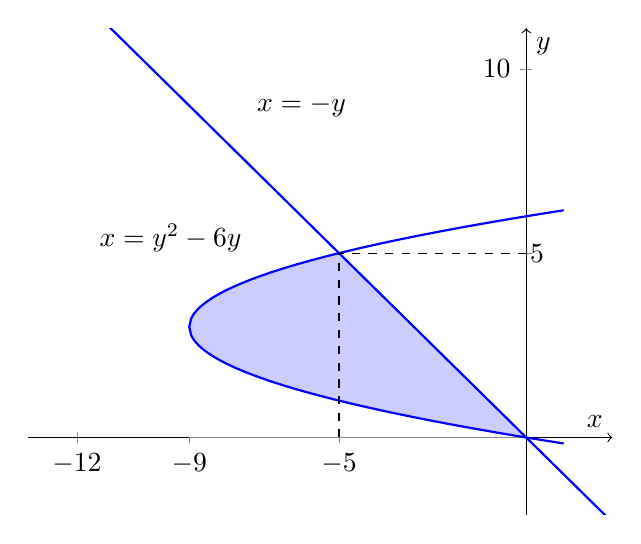
\begin{tikzpicture}
  \begin{axis}[
  width=9cm,
    yticklabel pos=right,
    axis lines = center,
    xlabel = $x$, ylabel = $y$,
    domain=-12:4,
    samples=300,
    ymin=-1, ymax=10,
    xmin=-12, xmax=1,
    enlargelimits=true,
    axis line style={->},
    ytick={10},
    xtick={-12, -9, -5},
    extra y ticks={5},
    extra y tick labels={5},
    extra y tick style={
        yticklabel pos=right,
        ticklabel style={anchor=west},
    },
    ]
    \addplot [
      domain=-9:-5,
      samples=200,
      fill=blue!20,
      draw=none,
    ]
    {sqrt(x+9)+3} \closedcycle;
    
    \addplot [
      domain=-5:0,
      samples=200,
      fill=blue!20,
      draw=none,
    ]
    {-x} \closedcycle;

    \addplot [
      domain=-9:0,
      samples=200,
      fill=white,
      draw=none,
    ]
    {-sqrt(x+9)+3} \closedcycle;
    
    \addplot[blue, thick, domain=-9:1, samples=200] {sqrt(x+9) + 3};
    \addplot[blue, thick, domain=-9:1, samples=200] {-sqrt(x+9) + 3};
    \addplot[blue, thick] {-x};

    \node at (axis cs:-6,9) {$x=-y$};
    \node at (axis cs:-9.5,5.4) {$x=y^2-6y$};

    \draw[dashed, black] (axis cs:-5,0) -- (axis cs:-5,5);
    \draw[dashed, black] (axis cs:0,5) -- (axis cs:-5,5);
  \end{axis}
\end{tikzpicture}\hspace{0.5cm}
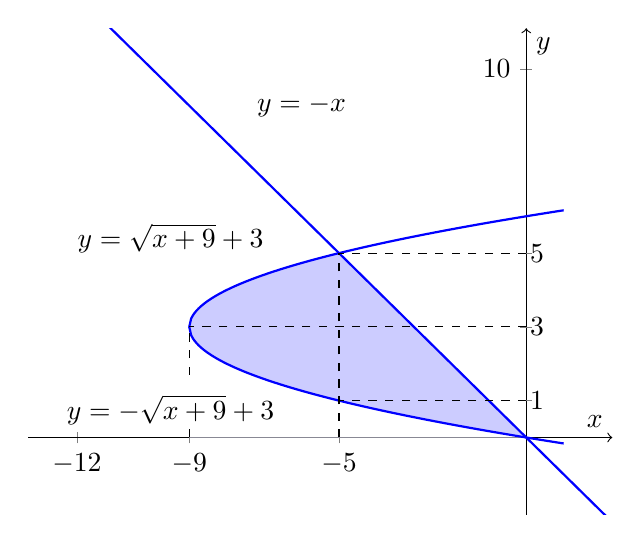
\begin{tikzpicture}
  \begin{axis}[
    width = 9cm,
    yticklabel pos=right,
    axis lines = center,
    xlabel = $x$, ylabel = $y$,
    domain=-12:4,
    samples=300,
    ymin=-1, ymax=10,
    xmin=-12, xmax=1,
    enlargelimits=true,
    axis line style={->},
    ytick={10},
    xtick={-12, -9, -5},
    extra y ticks={5,3,1},
    extra y tick labels={5,3,1},
    extra y tick style={
        yticklabel pos=right,
        ticklabel style={anchor=west},
    },
    ]
    \addplot [
      domain=-9:-5,
      samples=200,
      fill=blue!20,
      draw=none,
    ]
    {sqrt(x+9)+3} \closedcycle;
    
    \addplot [
      domain=-5:0,
      samples=200,
      fill=blue!20,
      draw=none,
    ]
    {-x} \closedcycle;

    \addplot [
      domain=-9:0,
      samples=200,
      fill=white,
      draw=none,
    ]
    {-sqrt(x+9)+3} \closedcycle;
    
    \addplot[blue, thick, domain=-9:1, samples=200] {sqrt(x+9) + 3};
    \addplot[blue, thick, domain=-9:1, samples=200] {-sqrt(x+9) + 3};
    \addplot[blue, thick] {-x};

    \node at (axis cs:-6,9) {$y=-x$};
    \node at (axis cs:-9.5,5.4) {$y=\sqrt{x+9} + 3$};
    \node at (axis cs:-9.5,0.75) {$y=-\sqrt{x+9} + 3$};

    \draw[dashed, black] (axis cs:-5,0) -- (axis cs:-5,5);
    \draw[dashed, black] (axis cs:0,3) -- (axis cs:-9,3);
    \draw[dashed, black] (axis cs:0,1) -- (axis cs:-5,1);
    \draw[dashed, black] (axis cs:0,5) -- (axis cs:-5,5);
    \draw[dashed, black] (axis cs:-9,0) -- (axis cs:-9,0.3);
    \draw[dashed, black] (axis cs:-9,1.7) -- (axis cs:-9,3);

  \end{axis}
\end{tikzpicture}
\end{center}

\hfill

\noindent (i) We'll take the integral along the $y$-axis. The lower and upper limits of the integral are 0 and 5, respectively.

\[A = \int_0^5[(-y)-(y^2-6y)]\,dy = \int_0^5(-y^2+5y)\,dy\]

\hfill

\noindent (ii) We have two different regions. $y=-x$ and $y=\sqrt{x-9}+3$ intersect at the point $(-5, 5)$. Therefore, we will write two separate integrals.

\begin{align*}
A&=\int_{-9}^{-5}\left[\left(\sqrt{x+9}+3\right) -\left(-\sqrt{x+9}+3\right)\right]\,dx + \int_{-5}^{0}\left[(-x) - \left(-\sqrt{x+9}+3\right)\right]\,dx\\\\
&=\int_{-9}^{-5}2\left(\sqrt{x+9}\right)\,dx + \int_{-5}^{0}\left(-x + \sqrt{x+9}-3\right)\,dx
\end{align*}

\newpage

\begin{center}
2019-2020 Fall Midterm (04/11/2019) Solutions\\
(Last update: 29/08/2025 21:51)
\end{center}

\noindent 1. Let $L$ be the value of the limit.

\[L = \lim_{x\to3^+}\cos(x-3)^{\ln\left(\frac{2x}{3}-2\right)}\]
\[\ln(L) =\ln\left( \lim_{x\to3^+}\cos(x-3)^{\ln\left(\frac{2x}{3}-2\right)}\right)\]

\hfill

\noindent Since $\cos(x-3)^{\ln(2x/3 -2)}$ is continuous for $x>3$, we can take the logarithm function inside the limit. Using the property of logarithms, we get:

\[\ln(L) =\lim_{x\to3^+}\left[ \ln\left(\cos(x-3)^{\ln\left(\frac{2x}{3}-2\right)}\right)\right] = \lim_{x\to3^+}\left[ \ln\left(\cos(x-3)\right)\ln\left(\frac{2x}{3}-2\right)\right]\quad[0 \cdot \infty]\]

\hfill

\noindent Rearrange the limit to obtain an indeterminate form. Afterwards, apply L'Hôpital's rule.

\begin{align*}&\lim_{x\to3^+}\left[ \ln\left(\cos(x-3)\right)\ln\left(\frac{2x}{3}-2\right)\right] = \lim_{x\to3^+}\frac{\ln\left(\frac{2x}{3}-2\right)}{1/ \ln\left(\cos(x-3)\right)} \quad \left[\frac00\right] \\\\&\overset{\text{L'H.}}{=} \lim_{x\to3^+}\frac{\displaystyle\frac1{\frac{2x}{3} - 2}\cdot \frac{2}{3}}{\displaystyle \left(-\ln^{-2}\displaystyle \cos(x-3)\right)\cdot \frac{1}{\cos(x-3)}\cdot(-\sin(x-3))}\\\\&= \lim_{x\to3^+} \displaystyle\frac{\ln^2(\cos(x-3))}{(x-3)\tan(x-3)} \quad\left[\frac00\right]\\\\&\overset{\text{L'H.}}{=} \lim_{x\to3^+} \frac{\displaystyle2\ln(\cos(x-3))\cdot\frac{1}{\cos(x-3)}\cdot(-\sin(x-3))}{\tan(x-3) + (x-3)\sec^2(x-3)}\\\\&=\lim_{x\to3^+}\frac{\displaystyle-2\ln(\cos(x-3))\sin(x-3)}{\sin(x-3) + (x-3)\sec(x-3)} \overset{u=x-3}{=} \lim_{u\to0^+}\left(\frac{\displaystyle-2\ln(\cos(u))\sin(u)}{\sin(u) + u\sec(u)} \cdot\frac{u}{u}\right)\\\\& = \frac{\displaystyle\lim_{u\to0^+}[-2\ln(\cos(u))]\cdot \lim_{u\to0^+}\frac{\sin(u)}{u}}{\displaystyle\lim_{u\to0^+}\sec(u)+\lim_{u\to0^+}\frac{\sin(u)}{u}}\quad \left[\lim_{u\to0} \frac{\sin(u)}u=1\right]\\\\&=\frac{\displaystyle\lim_{u\to0^+}[-2\ln(\cos(u))]}{\displaystyle\lim_{u\to0^+}\sec(u)+1}  =\frac{-2\ln(\cos(0))}{1+1} =\frac{-2\ln(1)}{2} = 0\end{align*}

\hfill

\noindent We found out that $\ln(L) = 0$. Therefore, $\boxed{L = 1}$.

\newpage

\noindent 2. To ensure continuity at $x=0$, the one-sided limit values must be equal to the value of the function at that point.

\[\lim_{x\to0^-}\frac{\tan ax}{\tan bx}=\lim_{x\to0^+}(ax+b)=f(0)=4\]

\hfill

\noindent The easy part is that we can calculate the limit from the right.

\[\lim_{x\to0^+} (ax+b) = 0+b = b\]

\hfill

\noindent Hence, $b=4$. To calculate from the left, we need another technique.

\begin{align*}
\lim_{x\to0^-} \frac{\tan ax}{\tan bx} &= \lim_{x\to0^-} \left(\frac{\sin ax}{\cos ax} \cdot \frac{\cos bx}{\sin bx} \cdot \frac{bx}{bx}\cdot \frac{ax}{ax}\right)\\\\&=\lim_{x\to0^-} \left(\frac{\sin ax}{ax} \right)\cdot \lim_{x\to0^-} \left(\frac1{ \frac{\sin bx}{bx}}\right)\ \cdot \lim_{x\to0^-} \left(\frac{\cos (bx) \cdot ax}{\cos(ax) \cdot bx}\right)\\\\&=1\cdot  \frac1{\displaystyle \lim_{x\to0^-}\frac{\sin bx}{bx}}\cdot \lim_{x\to0^-} \left(\frac{\cos (bx) \cdot a}{\cos(ax) \cdot b}\right)= 1\cdot 1\cdot\left(\frac{\cos(0) \cdot a}{\cos(0) \cdot b}\right)\\&=\frac ab
\end{align*}

\hfill

\noindent Now, set $\displaystyle \frac ab = b\,\rightarrow\, a= 16$. $\boxed{a=16,\,b=4}$

\hfill

\noindent 3. $-1 \leq \sin x\leq 1$, and $\sin x$ is continuous $\, \forall x\in \mathbb{R}$. $1-2x$ is continuous everywhere and takes any value in $\mathbb{R}$. Therefore, the equation $\sin x=1-2x$ must have at least one real solution by IVT, and the $y$-intercept is on the interval $[-1, 1]$.

\hfill

\noindent Let $f(x) = \sin x - 1 + 2x$ and $x_1$ be one solution to the equation. Then, the root must satisfy $|1-2x| \leq 1$. To disprove the existence of another root, we assume that $x_2$ is another distinct root. Since $f(x_1) = f(x_2) = 0$ and $f(x)$ is differentiable everywhere, by Rolle's theorem, there must exist a point $c$ such that

\[f'(c)=\frac{f(x_2)-f(x_1)}{x_2-x_1}=0\]

\hfill

\noindent Take the first derivative and calculate $f'(c)$

\[f'(c)=\cos c+2\]

\hfill

\noindent $-1\leq\cos x\leq 1$. Therefore, there is no such c that satisfies $f'(c) = 0$. This is a contradiction. By Rolle's theorem, there is \textit{only} one root satisfying $\sin x = 1-2x$.

\noindent 4. Let $f(t)$ and $g(t)$ represent the distance between Ship A and point O, and the distance between Ship B and point O, respectively. The distance between the ships can be represented using the Pythagorean theorem as follows:

\[D^2(t)=f^2(t)+g^2(t)\]

\hfill

\noindent Take the derivative of both sides.

\[2D\frac{dD}{dt} = 2f(t)f'(t) + 2g(t)g'(t)\]

\hfill

\noindent Solve for $\dfrac{dD}{dt}$.

\[
\frac{dD}{dt} = \frac{f(t)f'(t) + g(t)g'(t)}{\displaystyle D}
\]

\hfill

\noindent For $t=t_0$, we have $f(t_0)=60,\:g(t_0)=80,f'(t_0)=20,\:g'(t_0)=-25,\:D(t_0)=\sqrt{60^2+80^2}=100$. We may now find the rate of change of the distance at that time.

\[\frac{dD}{dt}\Bigg|_{t=t_0} = \frac{60\cdot 20 -80 \cdot 25}{\displaystyle 100} = \boxed{-8 \, \text{miles/hour}}\]

\hfill

\noindent 5. First off, find the domain. The expression is undefined when the denominator is zero. Therefore, $x\neq 0$. The only vertical asymptote occurs at $x = 0$.

\[\mathcal{D} = \mathbb{R} - \{0\}\]

\hfill

\noindent Let us find the limit at infinity and the limit at negative infinity.

\[\lim_{x\to\infty}\frac{\mathrm{e}^x}{x}\overset{\text{L'H.}}{=}\lim_{x\to\infty}\frac{\mathrm{e}^x}{1}=\infty\]

\[\lim_{x\to-\infty}\frac{\mathrm{e}^x}{x}=0\]

\hfill

\noindent The horizontal asymptote occurs only at $y=0$.

\hfill

\noindent Take the first derivative by applying the quotient rule.

\[y'=\frac{\mathrm{e}^x\cdot x-\mathrm{e}^x\cdot1}{x^2}=\frac{\mathrm{e}^x(x-1)}{x^2}\]

\hfill

\noindent $y'$ is undefined for $x=0$, and $y'=0$ for $x=1$. Since 0 is not in the domain, the \textit{only} critical point is $x=1$.

\hfill

\noindent Take the second derivative.

\[y''=\frac{[\mathrm{e}^x(x-1)+\mathrm{e}^x]x^2-\mathrm{e}^x(x-1)\cdot2x}{x^4}=\frac{\mathrm{e}^x(x^2-2x+2)}{x^3}\]

\hfill

\noindent There is no inflection point.

\hfill

\noindent Consider some values of the function. Eventually, set up a table and see what the graph looks like in certain intervals.

\[\,f(1) = \frac{\mathrm{e}^1}{1} = \mathrm{e}\]

\begin{center}
    \large
    \begin{tabular}{ |c| c c c| } 
    \hline
        $x$ & $(-\infty, 0)$ & $(0, 1)$ & $(1, \infty)$  \\
        \hline
        $y$ & $(-\infty, 0)$ & $(\infty, \mathrm{e})$ & $(\mathrm{e}, \infty)$\\
        \hline
        $y'$ sign & - & - & + \\
        \hline
        $y''$ sign & - & + & + \\
        \hline
    \end{tabular}
\end{center}

\hfill

\begin{center}
\begin{tikzpicture}
  \begin{axis}[
    axis lines = center,
    xlabel = $x$, ylabel = $y$,
    domain=-4:4,
    samples=800,
    ymin=-8, ymax=8,
    xmin=-4, xmax=4,
    restrict y to domain=-9:9,
    enlargelimits=true,
    axis line style={->},
    ytick={-8, -6,-4,e,4,6,8},
    xtick={-4,-3,-2,-1,1,2,3,4},
    yticklabels={-8, -6,-4,e,4,6,8},
    scale=1.5,
    ]
    \addplot[blue, thick] {e^x/x};

    \draw[dashed, red] (axis cs:0.04,-9) -- (axis cs:0.04,9);
    \draw[dashed, red] (axis cs:-5,0.04) -- (axis cs:5,0.04);
    \draw[dashed, black] (axis cs:0,e) -- (axis cs:1,e);
    \draw[dashed, black] (axis cs:1,0) -- (axis cs:1,e);

  \end{axis}
\end{tikzpicture}
\end{center}

\noindent 6.

\hfill

\noindent (a) Let $x= 3\tan u$, then $dx=3\sec^2u \,du$.

\begin{align}
\mathrm{I} = \int x^2\sqrt{9+x^2} \, dx &= \int (3\tan u)^2 \cdot\sqrt{9+(3\tan u)^2} \cdot3\sec^2(u)\,du \quad [1+ \tan^2u = \sec^2u] \nonumber\\\nonumber\\&=81\int\tan^2u \cdot \sec^3u \,du = 81\int \frac{\sin^2u}{\cos ^5 u}\, du = 81\int \frac{1-\cos^2u}{\cos^5u}\,du\nonumber\\\nonumber\\&=81\int\sec^5u\, du - 81\int \sec^3u\,du
\end{align}

\hfill

\noindent Find the left-hand integral in $(1)$ with integration by parts.

\begin{align*}
    w=\sec^3 u\,&\rightarrow\, dw = 3\sec^3u\tan u \,du\\
    dz=\sec^2u\,du\,&\rightarrow\, z = \tan u
\end{align*}
\[
\int\sec^5u \,du =\tan u \cdot \sec^3 u -3\int \tan^2u\cdot \sec^3 u\,du  = \tan u \cdot \sec^3 u - 3\int(\sec^5u- \sec^3u)\,du
\]

\hfill

\noindent The integral we want to evaluate appears on the right side. After a little algebra, we get:

\[\int\sec^5u \,du = \frac 14\cdot\tan u\cdot\sec^3 u + \frac 34\int\sec^3u\,du\]

\hfill

\noindent Rewrite $(1)$ and calculate the other integral in $(1)$ with integration by parts.

\begin{equation}
\mathrm{I} = \frac{81}4\cdot\tan u\cdot\sec^3 u - \frac {81}4\int\sec^3u\,du
\end{equation}

\begin{align*}
    w=\sec u\,&\rightarrow\, dw = \sec u\tan u \,du\\
    dz=\sec^2u\,du\,&\rightarrow\, z = \tan u
\end{align*}
\begin{align*}
\int\sec^3u\,du&=\tan u \cdot \sec u -\int \tan^2 u\sec u\, du = \tan u \cdot \sec u -\int \frac{1-\cos^2u}{\cos^3 u}\, du\\\\&= \tan u \cdot \sec u - \int \sec^3u \, du + \int \sec u \, du 
\end{align*}

\hfill

\noindent We encountered a similar case when calculating $\displaystyle \int\sec^5 u \, du$. So,

\[\int\sec^3u\,du= \frac12\cdot\tan u \cdot\sec u + \frac12\cdot\int \sec u\,du\]

\hfill

\noindent The integral of $\sec u$ with respect to $u$ is as follows. One can derive it with particular methods.

\begin{equation}\int\sec u \, du = \ln|\tan u + \sec u| + c_1,\,c_1\in\mathbb{R}
\end{equation}

\hfill

\noindent Rewrite (2) using (3).

\[\mathrm{I} = \frac{81}4\cdot\tan u\cdot\sec^3 u -\frac{81}{8} \cdot\tan u \cdot\sec u-\frac{81}{8}\cdot\ln|\tan u + \sec u| + c\]

\hfill

\noindent Recall that $x=3\tan u$, then $\displaystyle x^2 = 9\tan^2u = 9\sec^2u-9\,\rightarrow\, \sec u =\frac{\sqrt{x^2+9}}3$. The result is then as follows. Furthermore, we can omit the constant part to simplify.

\[\mathrm{I}=\frac{x\sqrt{x^2+9}}8\left(2x^2+9\right)-\frac{81}8\ln\left|\frac{x+\sqrt{x^2+9}}3\right| + c,\,c\in\mathbb{R}\]

\[\boxed{\mathrm{I}=\frac{x\sqrt{x^2+9}}8\left(2x^2+9\right)-\frac{81}8\ln\left|x+\sqrt{x^2+9}\right| + c,\,c\in\mathbb{R}}\]

\newpage

\noindent (b) Rewrite the expression. Then, let $u =\tan^2x + 1$. So, $du=2\tan x \sec^2 x\,dx$

\begin{align*}
\mathrm{I} &=\int\tan x \cdot\sec^6 x\, dx \quad\left[\tan^2x+1=\sec^2x\right] \\\\ &= \int\tan x\cdot\sec^2x\cdot(1+\tan^2x)^2 \,dx=\frac12\int u^2 \,du  = \frac{u^3}6 + c
\end{align*}

\[\boxed{\mathrm{I}=\frac{(\tan^2x+1)^3}{6} + c, \, c\in \mathbb{R}}\]

\noindent (c) This is an improper integral; we need to make use of the limit concept. The expression is undefined for $x=4$.

\begin{align*}
\mathrm{I} &= \int_4^8\frac1{(x-4)^3}\,dx = \lim_{\mathrm{R}\to4^+}\int_\mathrm{R}^8\frac1{(x-4)^3}\,dx=\lim_{\mathrm{R}\to4^+} \left[-\frac1{2(x-4)^2}\right]_\mathrm{R}^8\\\\&=\lim_{\mathrm{R}\to4^+} \left[-\frac1{32} + \frac1{(R-4)^2}\right]=\boxed\infty
\end{align*}

\hfill

\noindent (d) We'll use integration by parts.

\begin{align*}u=e^x\,&\rightarrow\,du=\mathrm{e}^x\,dx \\dv=\mathrm{e}^x\sin \mathrm{e}^x \,dx \,&\rightarrow\,v=-\cos\mathrm{e}^x\end{align*}
\begin{align*}\int\mathrm{e}^{2x}\sin\mathrm{e}^x\,dx&=(-\cos\mathrm{e}^x)\cdot\mathrm{e}^x-\int\mathrm{e}^x\cdot(-\cos\mathrm{e}^x)\,dx\\\\&=\boxed{-\mathrm{e}^x\cos \mathrm{e}^x +\sin \mathrm{e}^x + c, \,c \in \mathbb{R}} \end{align*}

\hfill

\noindent (e) We may utilize the tangent half-angle substitution, which is sometimes called the Weierstrass substitution. Let $\displaystyle t = \tan\left(\frac x2\right)$. After some mathematical operations, we get the following. One can later derive the formulas.

\[\sin x={\frac{2t}{1+t^{2}}}\quad\cos x={\frac{1-t^{2}}{1+t^{2}}}\quad dx={\frac2{1+t^{2}}}\,dt\]

\hfill

\noindent Rewrite the integral and apply partial fraction decomposition.

\begin{align}
\mathrm{I} &= \int\frac{dx}{\sin x - \cos x} = \int\frac{\frac2{1+t^2}}{\frac{2t}{1+t^2} -\frac{1-t^2}{1+t^2}}\,dt=\int\frac2{t^2+2t-1}\,dt=2\int\frac1{(t+1)^2-(\sqrt2)^2}\,dt\nonumber\\\nonumber\\&=2\int\frac 1{\left(t+1-\sqrt2\right)\left(t+1+\sqrt2\right)}\,dt=2\int\left( \frac A{t+1+\sqrt2} + \frac B{t+1-\sqrt2}\right)\,dt
\end{align}

\begin{align*}
A(t+1-\sqrt2)+B(t+1+\sqrt2)&=1\\
t(A+B)+A+B+\sqrt2(B-A)&=1\\
\therefore A+B=0\quad[\text{eliminate}\:t]\,&\rightarrow\,B-A=\frac1{\sqrt2}
\end{align*}

\[
\left.
\begin{array}{ll}
A+B=0\\
\displaystyle B-A=\frac1{\sqrt2}
\end{array}
\right\}
\quad A=-\frac1{2\sqrt2},\quad B=\frac1{2\sqrt2}
\]

\hfill

\noindent Plug the values of $A$ and $B$ into $(4)$.

\[\mathrm{I}=\frac{\sqrt2}2\int\left(\frac1{t+1-\sqrt2}-\frac1{t+1+\sqrt2}\right)\,dt=\frac{\sqrt2}2\ln\left(\frac{|t+1-\sqrt2|}{|t+1+\sqrt2|}\right) +c,\,c\in\mathbb{R}\]

\[\boxed{\mathrm{I}=\frac{\sqrt2}2\ln\left(\frac{\displaystyle\left|\tan\left(\frac x2\right)+1-\sqrt2\right|}{\displaystyle\left|\tan\left(\frac x2\right)+1+\sqrt2\right|}\right)+c,\quad c\in\mathbb{R}}\]

\hfill

\noindent 7.

\begin{center}
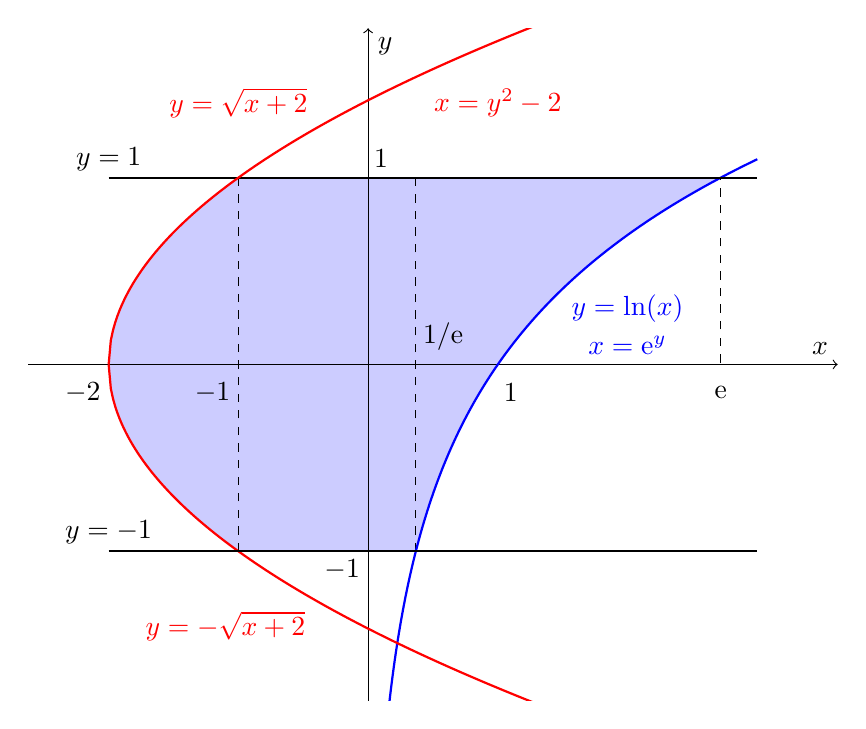
\begin{tikzpicture}
  \begin{axis}[
    scale=1.5,
    axis lines=center,
    xlabel={$x$},
    ylabel={$y$},
    xmin=-2.1, xmax=3.1,
    ymin=-1.5, ymax=1.5,
    samples=300,
    domain=-1:1,
    clip=true,
    ytick=\empty,
    xtick=\empty,
    enlargelimits=true,
    axis line style={->},
    xticklabel=\empty,
    yticklabel=\empty,
  ]

  \addplot [blue, thick, domain=1/e:1, draw=none, fill=blue!20] {ln(x)} \closedcycle;
  \addplot [blue, thick, domain=-1-0.01:1/e+0.01, draw=none, fill=blue!20] {-1} \closedcycle;
  \addplot [blue, thick, domain=-1-0.01:1+0.01, draw=none, fill=blue!20] {1} \closedcycle;
  \addplot [blue, thick, domain=-2:-1, draw=none, fill=blue!20] {sqrt(x+2)} \closedcycle;
  \addplot [blue, thick, domain=-2:-1, draw=none, fill=blue!20] {-sqrt(x+2)} \closedcycle;
  \addplot [blue, thick, domain=1:e, draw=none, fill=blue!20] {1} \closedcycle;
  \addplot [blue, thick, domain=1:e, draw=none, fill=white] {ln(x)} \closedcycle;
  
  \draw[black] (axis cs:0,-1) -- (axis cs:0,1);
  \draw[black] (axis cs:-2,0) -- (axis cs:e,0);
  \draw[white] (axis cs:e,0.01) -- (axis cs:e,1);
  \draw[dashed] (axis cs:-1,-1) -- (axis cs:-1,1);
  \draw[dashed] (axis cs:e,0.01) -- (axis cs:e,1);
  \draw[dashed] (axis cs:1/e,-1) -- (axis cs:1/e,1);

  \addplot [blue, thick, domain=0.1:3] {ln(x)};
  \addplot [thick, domain=-2:3] {1}; 
  \addplot [red, thick, domain=-2:3] {sqrt(x+2)};
  \addplot [red, thick, domain=-2:3] {-sqrt(x+2)};
  \addplot [thick, domain=-2:3] {-1};
  
  \node at (axis cs:e,-0.15) {$\mathrm e$};
  \node at (axis cs:1.1,-0.15) {$1$};
  \node at (axis cs:-2.2,-0.15) {$-2$};
  
  \node at (axis cs:0.1,1.1) {$1$};
  \node at (axis cs:-0.2,-1.1) {$-1$};
  
  \node at (axis cs:-1.2,-0.15) {$-1$};
  \node at (axis cs:1/e+0.21,0.15) {$1/\mathrm e$};
    
  \node[red] at (axis cs:1,1.4) {$x=y^2-2$};
  \node[red] at (axis cs:-1,1.4) {$y=\sqrt{x+2}$};
  \node[red] at (axis cs:-1.1,-1.4) {$y=-\sqrt{x+2}$};

  \node[blue] at (axis cs:2,0.3) {$y=\ln(x)$};
  \node[blue] at (axis cs:2,0.1) {$x=\mathrm e^y$};
  \node at (axis cs:-2,-0.9) {$y=-1$};
  \node at (axis cs:-2,1.1) {$y=1$};

  \end{axis}
\end{tikzpicture}\hspace{0.5cm}
\end{center}

\hfill

\noindent (i) The variable is $y$. Hence, the limits are $-1, 1$, respectively.

\[A=\int_{-1}^1\left[\mathrm{e}^y-(y^2-2)\right]\,dy\]

\hfill

\noindent (ii) We have three different regions. This leads us to take three different integrals.

\[A=\int_{-2}^{-1}\left[\sqrt{x+2}-(-\sqrt{x+2})\right]\,dx+\int_{-1}^{1/\mathrm{e}}\left[1-(-1)\right]\,dx+\int_{1/\mathrm{e}}^{\mathrm{e}}\left(1-\ln x\right)\,dx\]

\newpage

\begin{center}
2020-2021 Fall Midterm (30/11/2020) Solutions\\
(Last update: 29/08/2025 22:18)
\end{center}

\noindent 1. Let $L$ be the value of the limit. Since the expression is continuous for $x>0$, we can apply the logarithm function to each side of the equation. Then, we can swap the logarithm and the limit. Use the property of logarithms afterwards.

\[L=\lim_{x\to0^+}\left(\sqrt x\right)^{\ln\left(x+1\right)}\]

\[\ln(L)=\ln\left[\lim_{x\to0^+}\left(\sqrt x\right)^{\ln\left(x+1\right)}\right]=\lim_{x\to0^+}\ln\left[\left(\sqrt x\right)^{\ln\left(x+1\right)}\right]=\lim_{x\to0^+}\ln\left[\left(\sqrt x\right)^{\ln\left(x+1\right)}\right] \]
\[\ln\left(L\right)=\lim_{x\to0^+}\left[\ln\left(x+1\right)\cdot\ln\left(\sqrt x\right)\right] \quad\left[0\cdot\infty\right]\]

\hfill

\noindent Make it so the limit is in the form $\displaystyle \frac00$ or $\displaystyle \frac\infty\infty$ in order to apply the L'Hôpital's rule.

\begin{align*}\ln\left(L\right)&=\lim_{x\to0^+}\left[\frac{\ln\left(\sqrt x\right)}{\frac1{\ln\left(x+1\right)}}\right] \quad\left[\frac\infty\infty\right]\\\\&\overset{\text{L'H.}}{=}\lim_{x\to0^+}\left[\frac{\frac1{\sqrt x}\cdot\frac1{2\sqrt x}}{-\frac1{\ln^2\left(x+1\right)}\cdot \frac1{x+1}}\right]=\lim_{x\to0^+}\left[-\frac{\ln^2(x+1)\cdot(x+1)}{2x}\right]\\\\&=\lim_{x\to0^+}\left[-\frac{\ln^2(x+1)}{2x}\right] \cdot\lim_{x\to0^+} \left(x+1\right)=\lim_{x\to0^+}\left[-\frac{\ln^2(x+1)}{2x}\right]\quad\left[\frac00\right]\\\\&\overset{\text{L'H.}}{=}\lim_{x\to0^+}\left[-\frac{2\ln(x+1) \cdot\frac1{x+1}}2\right]=\lim_{x\to0^+}\left[\frac{\ln(x+1)}{x+1}\right]=\frac{\ln1}{1}=0\end{align*}

\hfill

\noindent $\ln(L)=0$, so $\boxed{L=1}$.

\hfill

\noindent 2. $\displaystyle \arctan\frac1x$ takes it values on $\displaystyle -\frac{\pi}2 \leq \arctan\frac1x \leq \frac{\pi}2$. Multiply each side by $x$, then we get $\displaystyle -\frac{x\pi}2 \leq x\arctan\frac1x \leq \frac{x\pi}2$. Take the limits of each side. By the squeeze theorem, we see that the limit of $\displaystyle x\arctan\frac1x$ at the point $x=0$ is $0$. This means that for $f(x)$, the limit from the right side also equals $0$.

\[\lim_{x\to 0}\left(-\frac{x\pi}2\right)\leq\lim_{x\to 0}\left(x\arctan\frac1x\right)\leq\lim_{x\to 0}\left(\frac{x\pi}2\right)\]
\[0\leq\lim_{x\to 0}\left(x\arctan\frac1x\right)\leq0\]
\[\therefore\lim_{x\to 0}\left(x\arctan\frac1x\right) = 0\]

\hfill

\noindent From the left side, the limit is equal to as follows.

\[\lim_{x\to0^-}\frac{x-\cos x}{x^2}=\lim_{x\to0^-}(x-\cos x)\cdot\lim_{x\to0^-}\frac1{x^2} =-\infty\]

\hfill

\noindent Continuity requires the equality of one-sided limits and the value of the function at that point. However, the one-sided limits are not equal; $0\neq-\infty$. Therefore, $f(x)$ is discontinuous at $x=0$.

\hfill

\noindent 3. Differentiate both sides implicitly.

\[\frac{d}{dx}\left(\cos y^2+xy+1\right)=\frac{d}{dx}(0)\]
\[-\sin y^2\cdot2y\frac{dy}{dx}+y+x\frac{dy}{dx}=0\]

\[\frac{dy}{dx}\left(-\sin y^2\cdot2y+x\right)=-y\]

\begin{equation}\frac{dy}{dx}= \frac y{\sin y^2 \cdot 2y - x}\end{equation}

\hfill

\noindent Evaluate $\displaystyle \frac{dy}{dx}$ at the point.

\begin{equation}\left.\frac{dy}{dx}\right|_{\left(\sqrt{\frac{2}{\pi}},-\sqrt{\frac{\pi}{2}}\right)} =\frac y{\sin y^2\cdot2y-x}=\frac{-\sqrt{\frac{\pi}{2}}}{\sin\left(\left(-\sqrt{\frac{\pi}{2}}\right)^2\right)\cdot2\left(-\sqrt{\frac{\pi}{2}}\right)-\sqrt{\frac{2}{\pi}}} =\frac{\sqrt{\frac{\pi}{2}}}{\sqrt{2\pi}+\sqrt{\frac{2}{\pi}}}\end{equation}

\hfill

\noindent Recall: $y-y_0 = m(x-x_0)$, where $m$ is the slope. Substitute $m$ with $(2)$ and find the tangent line.

\[\boxed{y+\sqrt{\frac{\pi}{2}}=\frac{\displaystyle\sqrt{\frac{\pi}{2}}}{\displaystyle\sqrt{2\pi}+\sqrt{\frac{2}{\pi}}}\left(x-\sqrt{\frac{2}{\pi}}\right)}\]

\hfill

\noindent 4. Let $S(t),\, V(t),\, a(t)$ represent the surface area, the volume, and the length of one side of the object, respectively, as a function of time. We may write the following.

\[S(t)=6a^2(t),\quad V(t)=a^3(t)\]

\hfill

\noindent Given that at $t=t_0$, $V(t_0) = 216, \,S'(t_0)=-36$. Using the relationship with the sides,

\begin{align*}
&V(t_0) = a^3(t_0)= 216\,\rightarrow\, a(t_0) = 6\\
&S'(t_0) = 12a(t_0)a'(t_0)=-36\\
&\therefore 12\cdot6\cdot a'(t_0)=-36 \,\rightarrow\, a'(t_0)=-\frac12
\end{align*}

\[\boxed{a'(t_0) = -\frac12\,\text{cm/h}}\]

\newpage

\noindent 5.

\hfill

\noindent (a) Let $f(x) = \mathrm{e}^x + x$. $f$ is continuous and differentiable for all $x\in\mathbb{R}$.

\[f(-1)=\mathrm{e}^{-1}-1=\frac1{\mathrm{e}}-1,\quad f(0)=\mathrm{e}-0=\mathrm{e}\]

\hfill

\noindent Since $f(-1) < 0$ and $f(0) > 0$ and $f$ is continuous on the interval $[-1, 0]$, by IVT, there is at least one point $x_1$ that satisfies $f(x_1) = 0$. Assume that there is another distinct root $x_2$. Rolle's theorem states that if $f$ is continuous on a particular interval with endpoints having the same function value, there exists a point $c$ on that interval such that $f'(c) = 0$ there.

\[f'(c)=\mathrm{e}^c+1\geq1\qquad\left[\mathrm{e}^c>0\right]\]

\hfill

\noindent This yields a contradiction. Therefore, there is \textit{only} one root.

\hfill

\noindent (b) The expression is defined $\forall x\in\mathbb{R}$. Let us find the limit at infinity and the limit at negative infinity.

\[\lim_{x\to\infty}\left(\mathrm{e}^x+x\right)=\infty\qquad\lim_{x\to-\infty}\left(\mathrm{e}^x+x\right)=-\infty\]

\hfill

\noindent There are no vertical or horizontal asymptotes. However, there is a slant asymptote. Attempt a long polynomial division and we will find that the slant asymptote is $y=x$. Verify with the following limit:

\[\lim_{x\to-\infty}\left[\left(\mathrm{e}^x+x\right)-x\right]=\lim_{x\to-\infty}\mathrm{e}^x=0\]

\hfill 

\noindent Take the first and second derivatives.

\[y'=\mathrm{e}^x+1,\quad y''=\mathrm{e}^x\]

\hfill 

\noindent We see that there are no critical or inflection points either. Now, set up a table and see what the graph looks like.

\begin{center}
    \large
    \begin{tabular}{ |c| c| } 
    \hline
        $x$ & $(-\infty, \infty)$\\
        \hline
        $y$ & $(-\infty, \infty)$\\
        \hline
        $y'$ sign & + \\
        \hline
        $y''$ sign & + \\
        \hline
    \end{tabular}
\end{center}

\hfill

\begin{center}
\begin{tikzpicture}
  \begin{axis}[
    axis lines = center,
    xlabel = $x$, ylabel = $y$,
    domain=-4:4,
    samples=200,
    ymin=-4, ymax=4,
    xmin=-4, xmax=4,
    axis line style={->},
    scale=1.3,
    ]
    \addplot[blue, thick] {e^x+x};
    
    \node[blue] at (1.8, 3.2) {$y=\mathrm e^x+x$};

    \draw[dashed, red] (axis cs:-5,-5) -- (axis cs:5,5);
  \end{axis}
\end{tikzpicture}
\end{center}

\noindent 6.
\begin{center}
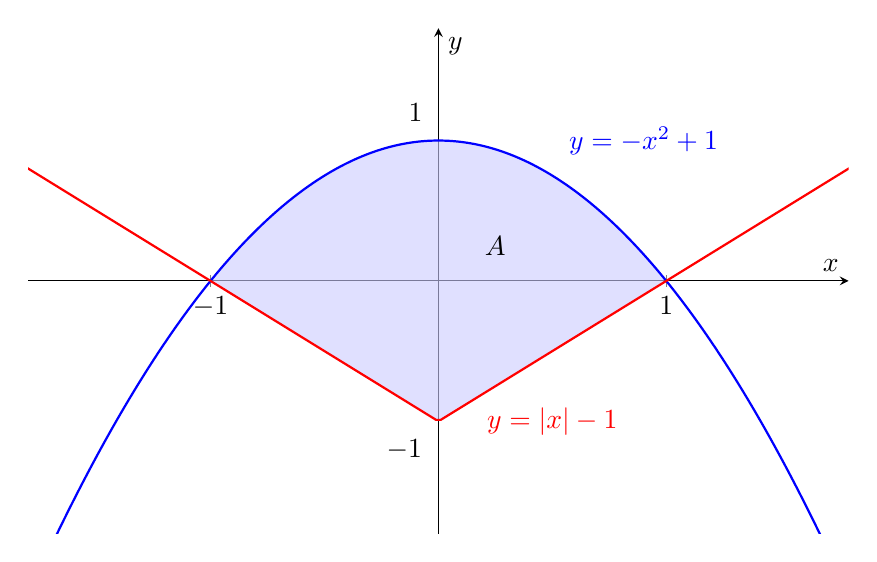
\begin{tikzpicture}
  \begin{axis}[
    axis lines = middle,
    xlabel = $x$,
    ylabel = $y$,
    domain=-2:2,
    samples=200,
    xtick={-2,-1,1,2},
    ytick={2,-2},
    ymin=-1.8, ymax=1.8,
    xmin=-1.8, xmax=1.8,
    width=12cm,
    height=8cm,
  ]

    \addplot [
      name path=upper,
      domain=-1:1,
      samples=200,
      draw=none
    ] {-x^2 + 1};

    \addplot [
      name path=lower,
      domain=-2:2,
      samples=200,
      draw=none
    ] {abs(x) - 1};

    \addplot [
      fill=blue!20,
      draw=none,
      opacity=0.6,
    ] fill between[of=upper and lower, soft clip={domain=-2:2}];

    \addplot [thick, blue] {-x^2 + 1};
    \addplot [thick, red] {abs(x) - 1};
    
    \node at (-0.1, 1.2) {$1$};
    \node at (-0.15, -1.2) {$-1$};
    
    \node[blue] at (0.9, 1) {$y=-x^2+1$};
    \node[red] at (0.5, -1) {$y=|x|-1$};
    
    \node at (0.25, 0.25) {$A$};

  \end{axis}
\end{tikzpicture}
\end{center}

\hfill

\noindent The area of the region is as follows.

\[A=\int_{-1}^1\left[(-x^2+1)-(|x|-1)\right]\,dx=\int_{-1}^0(-x^2+x +2)\,dx+\int_{0}^1(-x^2-x+2)\,dx\]

\hfill

\noindent 7. We'll use integration by parts.

\[
\left.
\begin{array}{ll}
\displaystyle\ln x=u\,\rightarrow\,\frac1x\,dx=du  \\
\displaystyle x\,dx= dv \,\rightarrow\,\frac{x^2}2=v
\end{array}
\right\}\quad
\begin{array}{ll}
\mathrm{I}&=\displaystyle\int x\ln x\,dx = \frac{x^2}2\cdot\ln x-\int\frac{x^2}2\cdot \frac1x \,dx \\\\&=\displaystyle\frac{x^2}2\cdot\ln x-\int\frac{x}2\,dx=\boxed{\frac{x^2}2\cdot\ln x - \frac{x^2}4+c,\,c\in\mathbb{R}}
\end{array}
\]

\newpage

\begin{center}
2021-2022 Fall Midterm (08/12/2021) Solutions\\
(Last update: 21/08/2025 16:06)
\end{center}

\noindent 1.

\hfill

\noindent (a) Determine one-sided limits.

\[\lim_{x\to-2^+}\frac{\left|x+2\right|}{\left|x\right|-2}=\lim_{x\to-2^+}\frac{x+2}{-x-2}=-1,\quad\quad\lim_{x\to-2^-}\frac{\left|x+2\right|}{\left|x\right|-2}=\lim_{x\to-2^-}\frac{-(x+2)}{-x-2}=1\]

\[\lim_{x\to-2^+}\frac{\left|x+2\right|}{\left|x\right|-2}\neq\lim_{x\to-2^-}\frac{\left|x+2\right|}{\left|x\right|-2}\implies\boxed{\text{The limit does not exist at }x=-2.}\]

\hfill

\noindent (b) We can separate the limit into two limits because we are going to demonstrate that each limit exists individually.

\begin{align}\lim_{x\to0}\frac{x^4\sin(1/x)}{\sin\left(x^2\right)}=\lim_{x\to0}\frac{x^2}{\sin\left(x^2\right)}\cdot\lim_{x\to0}x^2\sin\left(\frac1x\right)\end{align}

\hfill

\noindent The left-hand limit in $(1)$ is a standard form. Recall $\displaystyle\lim_{u\to0}\frac{\sin u}u=0$.

\[\lim_{x\to0}\frac{x^2}{\sin\left(x^2\right)}=\lim_{x\to0}\frac1{\displaystyle\frac{\sin\left(x^2\right)}{x^2}}=\frac1{\displaystyle\lim_{x\to 0}\frac{\sin\left(x^2\right)}{x^2}}=\frac11=1\]

\hfill

\noindent The right-hand limit in $(1)$ can be evaluated using the squeeze theorem. The trigonometric function $\displaystyle\sin\left(\frac1x\right)$ is continuous everywhere except at $x=0$.

\[-1\leq\sin\left(\frac1x\right)\leq1\]

\[-x^2\leq x^2\sin\left(\frac1x\right)\leq x^2\]

\[\lim_{x\to0}-x^2=\lim_{x\to0}x^2=0\implies\lim_{x\to0}x^2\sin\left(\frac1x\right)=0\]

\hfill

\noindent Plug the values of the limits into $(1)$ and find the result.

\[\lim_{x\to0}\frac{x^2}{\sin\left(x^2\right)}\cdot\lim_{x\to0}x^2\sin\left(\frac1x\right)=1\cdot0=\boxed0\]

\hfill

\noindent (c) Notice that this is the definition of the derivative at some point. Let $f(x)=\arccos x$. Then $\displaystyle f'(x) =\frac{-1}{\sqrt{1-x^2}}$.

\[\lim_{x\to0}=\frac{\arccos x -\frac\pi3}{x-\frac12}=\lim_{x\to0}\frac{f(x)-f\left(\frac12\right)}{x-\frac12}=f'\left(\frac12\right)=\frac{-1}{\sqrt{1-\left(\frac12\right)^2}}=\boxed{-\frac{2\sqrt3}{3}}\]

\newpage

\noindent (d) Expand the expression by multiplying and dividing by its conjugate.

\begin{align*}\lim_{x\to-\infty}x+\sqrt{x^2-x-4}&=\lim_{x\to-\infty}\left[\left(x+\sqrt{x^2-x-4}\right)\cdot\frac{x-\sqrt{x^2-x-4}}{x-\sqrt{x^2-x-4}}\right]\\\\&=\lim_{x\to-\infty}\frac{x^2-\left(x^2-x-4\right)}{x-\sqrt{x^2-x-4}}=\lim_{x\to-\infty}\frac{x+4}{x-\sqrt{x^2-x-4}}\\\\&=\lim_{x\to-\infty}\frac{x\left(1+\frac4x\right)}{x-\left|x\right|\sqrt{1-\frac1x-\frac4{x^2}}}=\lim_{x\to-\infty}\frac{x\left(1+\frac4x\right)}{x\left(1+\sqrt{1-\frac1x-\frac4{x^2}}\right)}\\\\&=\lim_{x\to-\infty}\frac{1+\frac4x}{1+\sqrt{1-\frac1x-\frac4{x^2}}}=\frac{1+0}{1+\sqrt{1-0-0}}=\boxed{\frac12}\end{align*}

\hfill

\noindent 2. Let $r,\:h$ represent the radius and height of the cylinder, respectively, for both sections. The volume of the cylinder is given by

\[V=\pi r^2h\]

\noindent The formula for $V$ is continuous and bounded when written as a function of height. According to the extreme value theorem, extrema must exist on the boundary or at critical points.

\hfill

\noindent (a) If this cylinder is vertically placed inside the hemisphere, using the Pythagorean theorem, we get the following relationship.

\[r^2+h^2=3^2\implies r^2=9-h^2\]

\hfill

\noindent Rewrite the volume formula by eliminating $r$.

\[V(h)=\pi\cdot h\cdot(9-h^2)=\pi\left(9h-h^3\right)\implies 0\leq h\leq3\]

\hfill

\noindent To maximize the volume, we need to determine the extrema of $V$ by taking the first derivative.

\[V'(h)=\pi\left(9-3h^2\right)=0\implies 3h^2=9\implies h=\sqrt3\]

\noindent Check the endpoints.

\[V(0)=0,\quad V(3)=0\]

\hfill

\noindent Since $h=\sqrt3,$ $r=\sqrt{9-\left(\sqrt3\right)^2}=\sqrt6$. The volume is then

\[V=\pi r^2 h=\pi\left(\sqrt6\right)^2\cdot\sqrt3=\boxed{6\pi\sqrt3}\]

\hfill

\noindent (b) If the cylinder is placed horizontally, using the Pythagorean theorem, we get the following relationship.

\[\left(\frac h2\right)^2+\left(2r\right)^2=3^2\implies r^2=\frac14\left(9-\frac{h^2}4\right)\]

\hfill

\noindent Rewrite the volume formula.

\[V(h)=\pi\cdot\frac14\left(9-\frac{h^2}4\right)\cdot h\implies0\leq h\leq6\]

\hfill

\noindent Take the first derivative and find the extrema.

\[V'(h) =\frac\pi4\left(9-\frac{3h^2}4\right)=0\implies h=2\sqrt3\]

\hfill

\noindent Check the endpoints.

\[V(0)=0,\quad V(6)=0\]

\hfill

\noindent Since $h=2\sqrt3,$ $r=\sqrt{\frac14\left(9-\frac{(2\sqrt3)^2}4\right)}=\frac{\sqrt6}2$. The volume is then

\[V=\pi r^2 h=\pi\cdot\left(\frac{\sqrt6}2\right)^2\cdot2\sqrt3=\boxed{3\pi\sqrt3}\]

\hfill

\noindent 3. Let $V(t),\:h(t)$ represent the volume and height of the gas in the cylinder as a function of time, respectively. The volume of a right circular cylinder can be expressed as follows.

\[V(t)=\pi\cdot r^2\cdot h(t)\]

\hfill

\noindent Take the derivative of both sides with respect to $t$.

\[V'(t)=\pi r^2\cdot h'(t)\]

\hfill

\noindent It is given that $2r=10\text{ cm},\: h'(t)=-7\text{ cm/s}$. Therefore, $r=5$ cm. The rate of change of volume at that moment is

\[V'(t)=25\pi\cdot(-7)=\boxed{-175\pi\text{ cm}^2\text{/s}}\]

\hfill

\noindent 4.

\hfill

\noindent (a) Let $L$ be the value of the limit. Then we can take the logarithm of both sides. After that, we may take the logarithm of the expression inside the limit. The expression is continuous for $x\neq0$.

\[L=\lim_{x\to0}\left(\frac{\sin x}x\right)^{1/x^2}\]

\[\ln(L) = \ln\left[\lim_{x\to0}\left(\frac{\sin x}x\right)^{1/x^2}\right]=\lim_{x\to0}\ln\left[\left(\frac{\sin x}x\right)^{1/x^2}\right]=\lim_{x\to0}\frac{\ln\left(\frac{\sin x}x\right)}{x^2}\]

\hfill

\noindent Recall that $\displaystyle \lim_{x\to0}\frac{\sin x}x=1$. Therefore, the limit is in the indeterminate form $0/0$. Apply L'Hôpital's rule where $0/0$ forms occur.

\begin{align*}
\ln(L)&=\lim_{x\to0}\frac{\ln\left(\frac{\sin x}x\right)}{x^2}\overset{\text{L'H.}}{=}\lim_{x\to0}\frac{\displaystyle\frac1{\frac{\sin x}x}\cdot\frac{\cos x\cdot x-\sin x\cdot1}{x^2}}{2x}=\lim_{x\to0}\frac{x\cos x-\sin x}{2x^2\cdot\sin x}\quad\left[\frac00\right]\\\\&\overset{\text{L'H.}}{=}\lim_{x\to0}\frac{1\cdot\cos x+x(-\sin x)-\cos x}{4x\cdot\sin x+2x^2\cdot\cos x}=\lim_{x\to0}\frac{-\sin x}{4\sin x+2x\cos x}\quad\left[\frac00\right]\\\\&\overset{\text{L'H.}}{=}\lim_{x\to0}\frac{-\cos x}{4\cos x+2\cos x+2x(-\sin x)}=\frac{-\cos0}{4\cos0+2\cos0-2\cdot0\cdot\sin0}=-\frac16
\end{align*}

\noindent If $\displaystyle \ln(L)=-\frac16$, then $\boxed{L=\mathrm{e}^{\textstyle-\frac16}}$.

\hfill

\noindent (b)
\[\frac xy=\cos(\pi xy)\implies x=y\cos(\pi xy)\]

\hfill

\noindent Differentiate each side.

\[1=y'\cdot\cos(\pi xy)+y\cdot(-\sin(\pi xy))\cdot\pi(1\cdot y+xy')\]
\[1=y'\cos(\pi xy)-\pi y^2\sin(\pi xy)-\pi xyy'\sin(\pi xy)\]
\[1+\pi y^2\sin(\pi xy)=y'\left[\cos(\pi xy)-\pi xy\sin(\pi xy)\right]\]

\[y'=\frac{1+\pi y^2\sin(\pi xy)}{\cos(\pi xy)-\pi xy\sin(\pi xy)}\]

\noindent Calculate $y'$ at the point $(-1,1)$.

\[y' = \frac{1+\pi\cdot\sin(-\pi)}{\cos(-\pi)+\pi\sin(-\pi)}=-1\]

\hfill

\noindent Recall the tangent line formula: $y-y_0=m(x-x_0)$, where $m$ is basically the derivative at the point $(-1,1)$. The tangent line is as follows.

\[y-1=-1(x+1)\implies\boxed{y=-x}\]

\newpage

\noindent 5. The expression is defined $\forall x\in \mathbb{R}- \{-1\}$. Let us find the limit at infinity and the limit at negative infinity.

\[\lim_{x\to\infty}\frac{2x^2}{(x+1)^2}\overset{\text{L'H.}}{=}\lim_{x\to\infty}\frac{4x}{2(x+1)}\overset{\text{L'H.}}{=}\lim_{x\to\infty}\frac42=2\quad\quad\lim_{x\to-\infty}\frac{2x^2}{(x+1)^2}=2\]

\hfill

\noindent The \textit{only} horizontal asymptote is $y=2$ and the \textit{only} vertical asymptote is $x=-1$.

\hfill 

\noindent Take the first derivative.

\[y'=\frac{4x\cdot(x+1)^2-2x^2\cdot2(x+1)}{(x+1)^4}=\frac{4x}{(x+1)^3}\]

\hfill

\noindent The \textit{only} critical point occurs at $x=0$.

\hfill 

\noindent Take the second derivative.

\[y''=\frac{4\cdot(x+1)^3-4x\cdot3(x+1)^2}{(x+1)^6}=\frac{4-8x}{(x+1)^4}\]

\hfill 

\noindent The \textit{only} inflection point occurs at $\displaystyle x=\frac12$.

\hfill 

\noindent Eventually, consider some values of the function, such as the $x$- and $y$-intercepts, and set up a table.

\[f(0) = 0, \quad f\left(\frac12\right)=\frac29\]

\begin{center}
    \large
    \begin{tabular}{ |c| c c c c| } 
    \hline
        $x$ & $(-\infty,-1)$ & $(-1,0)$ & $\left(0,\frac12\right)$ & $\left(\frac12,\infty\right)$ \\
        \hline
        $y$ & $(2,\infty)$ & $(0,\infty)$ & $\left(0,\frac29\right)$ & $\left(\frac29,2\right)$ \\
        \hline
        $y'$ sign & + & - & + & + \\
        \hline
        $y''$ sign & + & + & + & - \\
        \hline
    \end{tabular}
\end{center}

\hfill

\begin{center}
\begin{tikzpicture}
  \begin{axis}[
    axis lines = center,
    xlabel = $x$, ylabel = $y$,
    domain=-6:10,
    samples=300,
    ymin=-0.5, ymax=10,
    xmin=-6, xmax=6,
    yticklabels={,,,4,6,8,10},
    axis line style={->},
    scale=1.5,
    clip=true,
    restrict y to domain=0:15,
    ]
    \addplot[blue, thick] {(2*x*x)/((x+1)*(x+1))};

    \draw[dashed, red] (axis cs:-10,2) -- (axis cs:10,2);
    \draw[dashed, red] (axis cs:-1,0) -- (axis cs:-1,10);
    \draw[dashed] (axis cs:0.5,0) -- (axis cs:0.5,2/9);
    \draw[dashed] (axis cs:0,2/9) -- (axis cs:0.5,2/9);
    
    \node at (0.5, -0.3) {$0.5$};
    \node at (0.5, 0.8) {$2/9$};
    \node at (-1, -0.3) {$-1$};
    \node at (0.25, 2.3) {$2$};
  \end{axis}
\end{tikzpicture}
\end{center}

\noindent 6. $g$ is continuous and differentiable everywhere since it is a polynomial.

\hfill

\noindent Since $g(-1) = -2 < 0$ and $g(0)=1>0$, by IVT, there is at least one $c_1\in(-1,0)$ such that $g(c_1)=0$.

\hfill

\noindent Assume that $g$ has another root $c_2$, i.e., $g(c_2)=0$. Since $g$ is continuous on $[c_1, c_2]$ and differentiable on $(c_1,c_2)$, by MVT, there exists a $d\in(c_1,c_2)$ such that

\[g'(d)=\frac{g(c_2)-g(c_1)}{c_2-c_1}=0\]

\hfill

\noindent But, we have

\[g'(x) = 7x^6 + 3x^2 + 1\geq 0+0+1=1>0\]

\hfill

\noindent So, $g'(x)$ cannot be $0$. This yields a contradiction. Therefore, $g$ has only one root.

\newpage

\begin{center}
2022-2023 Fall Midterm (23/11/2022) Solutions\\
(Last update: 29/08/2025 22:59)
\end{center}

\noindent 1.

\hfill

\noindent (a) Find the one-sided limits.
\[\lim_{x\to 0^+} \frac{\left|\sin x\right|}{x}=\lim_{x\to 0^+}\frac{\sin x}{x}=1,\quad\quad \lim_{x\to 0^-} \frac{\left|\sin x\right|}{x}=\lim_{x\to0^-}\left(-\frac{\sin x}{x}\right)=-\lim_{x\to0^-}\frac{\sin x}{x}=-1\]

\hfill

\noindent The one-sided limits are not equal. Therefore, the limit does not exist.

\hfill

\noindent (b) We have $-1\leq\cos(1/x)\leq1$ for all $x\in\mathbb R-\{0\}$. So, $\mathrm{e}^{-1}\leq\mathrm{e}^{\cos(1/x)}\leq\mathrm{e}^1$.
\[x\mathrm{e}^{-1}\leq x\mathrm{e}^{\cos(1/x)}\leq x\mathrm{e}\implies\lim_{x\to0^+} x\mathrm{e}^{-1}=\lim_{x\to0^+}x\mathrm{e}=0\implies\lim_{x\to0^+}x\mathrm{e}^{\cos(1/x)}=\boxed0\]

\noindent By the squeeze theorem, the limit is 0.

\hfill

\noindent (c)
\begin{align*}L&=\displaystyle\lim_{x\to0}\frac{\sqrt{1+\tan x}-\sqrt{1-\sin x}}{x^3}
\\\\&=\lim_{x\to0}\left(\frac{\sqrt{1+\tan x}-\sqrt{1-\sin x}}{x^3}\cdot\frac{\sqrt{1+\tan x}+\sqrt{1-\sin x}}{\sqrt{1+\tan x}+\sqrt{1-\sin x}}\right)\\\\&=\lim_{x\to0}\frac{(1+\tan x)-(1-\sin x)}{x^3\cdot\left(\sqrt{1+\tan x}+\sqrt{1-\sin x}\right)}=\lim_{x\to0}\frac{\tan x+\sin x}{x^3\cdot\left(\sqrt{1+\tan x}+\sqrt{1-\sin x}\right)}\\\\&=\lim_{x\to0}\frac{\sin x+\sin x\cdot\cos x}{\cos x\cdot x^3\cdot\left(\sqrt{1+\tan x}+\sqrt{1-\sin x}\right)}\\\\&=\lim_{x\to0}\frac{1+\cos x}{\cos x\cdot x^2\cdot\left(\sqrt{1+\tan x}+\sqrt{1-\sin x}\right)}\cdot\lim_{x\to0}\frac{\sin x}{x}\quad\left[\lim_{x\to0}\frac{\sin x}x=1\right]\\\\&=\lim_{x\to0}\left[\frac{1+\cos x}{\cos x\cdot x^2\cdot\left(\sqrt{1+\tan x}+\sqrt{1-\sin x}\right)}\cdot\frac{1-\cos x}{1-\cos x}\right]\\\\&=\lim_{x\to0}\left[\frac{1-\cos^2x}{\cos x\cdot x^2\cdot(1-\cos x)\cdot\left(\sqrt{1+\tan x}+\sqrt{1-\sin x}\right)}\right]\quad\left[\sin^2x+\cos^2x=1\right]\\\\&=\lim_{x\to0}\frac{\sin^2x}{x^2}\cdot\lim_{x\to0}\frac1{\cos x\cdot(1-\cos x)\cdot\left(\sqrt{1+\tan x}+\sqrt{1-\sin x}\right)}\\\\&=\lim_{x\to0}\frac1{\cos x}\cdot\lim_{x\to0}\frac1{1-\cos x}\cdot\lim_{x\to0}\frac1{\sqrt{1+\tan x}+\sqrt{1-\sin x}}=1\cdot\lim_{x\to0}\frac1{1-\cos x}\cdot\frac12 =\boxed{\infty}\end{align*}

\hfill

\noindent 2. Let $g(t),\,f(t)$ represent the distance between point $A$ and point $B$, and the distance between point $A$ and the balloon, respectively. We may express the angle as follows.

\[\theta(t)=\arctan{\frac{f(t)}{g(t)}}\]

\hfill

\noindent The first derivative of $\theta$ gives the rate of change of the angle. Apply the chain rule accordingly.

\[\theta'(t)=\frac1{\displaystyle 1+\frac{f^2(t)}{g^2(t)}}\cdot\frac{f'(t)\cdot g(t) - f(t) \cdot g'(t)}{g^2(t)}=\frac{f'(t)\cdot g(t) - f(t) \cdot g'(t)}{g^2(t)+f^2(t)}\]

\hfill

\noindent At $t=t_0$, $f(t_0)= 200,\,g(t_0) =100,\,f'(t_0)=5,\,g'(t_0) = 0$. The reason why $g'(t_0) = 0$ is that the distance between the points does not change over time. Calculate $\theta'(t_0)$.

\[\theta'(t_0)=\frac{5\cdot 100 - 200 \cdot 0}{100^2+200^2}=\frac{500}{50000}=\boxed{\frac1{100}\,\mathrm{rad/s}} \]

\hfill

\noindent 3.

\hfill

\noindent (a) Let $f(x)$ be continuous on $[a,b]$ and differentiable on $(a,b)$. The IVT states that since $f$ is continuous on the interval, $f$ takes any value on $[f(a), f(b)]$. The MVT states that since $f$ is differentiable on the interval provided the continuity, there is at least one point such that the slope of the line that passes through the endpoints is equal to the slope of the line that is tangent to that point.

\hfill

\noindent (b) Let $f(x) = x^{123}+2x^{85} + 3x^{17} + 4x-1$. Since this is a polynomial expression, $f$ is continuous and differentiable everywhere. Arbitrarily choose $x=-1$ and $x=1$ to make calculations easy. By IVT, $f$ takes any value on $[f(-1), f(1)]$.

\[f(-1) = -11,\quad f(1) =9\]

\hfill

\noindent $f$ must have at least one root $x_1$ on $[-1, 1]$ by IVT. Now, we need to prove that there is \textit{only} one. We assume that there is another distinct root $x_2$. Since $f(x_1) = f(x_2) = 0$, at some point $c$, the first derivative of the function at this point is $0$.

\[f'(c) = 123x^{122}+170x^{84} + 51x^{16} + 4 \geq 0+ 0+ 0+ 4 = 4\]

\hfill

\noindent $f'(c)>0$. However, this is a contradiction. Therefore, there is \textit{only} one root.

\hfill

\noindent 4. Differentiate both sides.

\[\frac d{dx}\left[\sin(y^2\mathrm{e}^{2x})+\sqrt\pi y\right]=\frac{d}{dx}\left(x^2+\pi\right)\]
\[\cos\left(y^2\mathrm{e}^{2x}\right)\cdot\left(2y{\frac{dy}{dx}\mathrm{e}^{2x}}+y^2\mathrm{e}^{2x}\cdot2\right)+\sqrt\pi\frac{dy}{dx}=2x\]
\[2y{\mathrm{e}^{2x}}\cos\left(y^2\mathrm{e}^{2x}\right)\frac{dy}{dx}+2y^2\mathrm{e}^{2x}\cos\left(y^2\mathrm{e}^{2x}\right)+\sqrt\pi\frac{dy}{dx}=2x\]
\[\frac{dy}{dx}\left[2y\mathrm{e}^{2x}\cos\left(y^2\mathrm{e}^{2x}\right)+\sqrt\pi\right]=2x-2y^2{\mathrm{e}^{2x}}\cos\left(y^2\mathrm{e}^{2x}\right)\]

\begin{equation}\frac{dy}{dx}=\frac{2x-2y^2{\mathrm{e}^{2x}}\cos\left(y^2\mathrm{e}^{2x}\right)}{2y\mathrm{e}^{2x}\cos\left(y^2\mathrm{e}^{2x}\right)+\sqrt\pi}\end{equation}

\hfill

\noindent Evaluate (1) at $\left(0, \sqrt\pi\right)$.

\[\left.\frac{dy}{dx}\right|_{\left(0, \sqrt\pi\right)}=\frac{2\cdot0-2\left(\sqrt\pi\right)^2{\mathrm{e}^{0}}\cos\left(\left(\sqrt\pi\right)^2\mathrm{e}^{0}\right)}{2\sqrt\pi\mathrm{e}^{0}\cos\left(\left(\sqrt\pi\right)^2\mathrm{e}^{0}\right)+\sqrt\pi}=\frac{2\pi}{-\sqrt\pi}=-2\sqrt\pi\]

\hfill

\noindent Use the straight line formula. $y-y_0=m(x-x_0)$, where $m=\left.\dfrac{dy}{dx}\right|_{\left(0,\sqrt\pi\right)}$

\[\boxed{y=\sqrt\pi(1-2x)}\]

\hfill

\noindent 5. Let $L$ be the value of the limit.

\[L=\lim_{x\to\infty}\left(\frac{\ln x}x\right)^{1/x}\qquad\left[\infty^0\right]\]
\[\ln(L)=\ln\left[\lim_{x\to\infty}\left(\frac{\ln x}x\right)^{1/x}\right]\]

\hfill

\noindent Take the logarithm inside the limit because the expression is continuous for $x>0$.

\begin{align*}\ln(L)&=\lim_{x\to\infty}\ln\left[\left(\frac{\ln x}x\right)^{1/x}\right]=\lim_{x\to \infty}\left[\frac{\ln\left(\frac{\ln x}x\right)}x\right]\quad\left[\frac\infty\infty\right]\\\\&\overset{\text{L'H.}}{=}\lim_{x\to\infty} \frac{\dfrac1{\frac{\ln x}{x}}\cdot\dfrac{\frac1x\cdot x-\ln x\cdot1}{x^2}}{1}=\lim_{x\to\infty}\left({\frac x{\ln x}\cdot\frac{1-\ln x}{x^2}}\right)=\lim_{x\to\infty}\frac{1-\ln x}{x\ln x}\\\\&=\lim_{x\to\infty}\frac1{x\ln x}-\lim_{x\to\infty}\frac{\ln x}{x\ln x}=0-\lim_{x\to\infty}\frac1x=0\end{align*}

\hfill

\noindent If $\ln(L) = 0$, then $\boxed{L = 1}$.

\hfill

\noindent 6. First off, find the domain. The expression is undefined when the denominator is zero. Therefore, $(x-1)^2\neq0\,\rightarrow\,x\neq1$. The only vertical asymptote occurs at $x = 1$.

\[\mathcal{D}=\mathbb{R}-\{1\}\]

\hfill

\noindent Let us find the limit at infinity.

\[\lim_{x\to \infty}\frac{x^2-2}{(x-1)^2}\overset{\text{L'H.}}{=}\lim_{x\to \infty}\frac{2x}{2(x-1)}\overset{\text{L'H.}}{=}\lim_{x\to\infty}\frac{2}{2}=1\]

\noindent Similarly,

\[\lim_{x\to-\infty}\frac{x^2-2}{(x-1)^2}=1\]

\hfill

\noindent The horizontal asymptote occurs only at $y=0$.

\hfill

\noindent Take the first derivative by applying the quotient rule.

\[y'=\frac{(2x)\cdot(x-1)^2-\left(x^2-2\right)\cdot2(x-1)}{(x-1)^4}=\frac{4-2x}{(x-1)^3}\]

\hfill

\noindent $y'$ is undefined for $x=1$, and $y'=0$ for $x=2$. Since $1$ is not in the domain, the \textit{only} critical point is $x = 2$.

\hfill

\noindent Take the second derivative.

\[y''=\frac{(-2)\cdot(x-1)^3-(4-2x)\cdot3(x-1)^2}{(x-1)^6}=\frac{4x-10}{(x-1)^4}\]

\hfill

\noindent The only inflection point occurs at $x=\dfrac52$.

\hfill

\noindent Consider some values of the function. Eventually, set up a table and see what the graph looks like in certain intervals.

\[\,f\left(-\sqrt2\right)=f\left(\sqrt2\right)=0,\:f(0)=-2,\:f(2)=2,\:f(5/2)=17/9\]

\begin{center}
    \large
    \begin{tabular}{ |c| c c c c c c c| } 
    \hline
        $x$ & $\left(-\infty, -\sqrt2\right)$ & $\left(-\sqrt2, 0\right)$&$\left(0, 1\right)$ & $\left(1,\sqrt2\right)$ & $\left(\sqrt2, 2\right)$ & $\left(2, \frac52\right)$ & $\left(\frac52, \infty\right)$  \\
        \hline
        $y$ & $(0, 1)$ &$(-2,0)$ & $(-\infty, -2)$& $(-\infty, 0)$& $(0, 2)$& $\left(\frac{17}9, 2\right)$& $\left(1, \frac{17}9\right)$\\
        \hline
        $y'$ sign & - & - & - &+&+&-&- \\
        \hline
        $y''$ sign & - &- &-&-&-&-&+ \\
        \hline
    \end{tabular}
\end{center}

\hfill

\begin{center}
\begin{tikzpicture}
  \begin{axis}[
    axis lines = center,
    xlabel = $x$, ylabel = $y$,
    domain=-12:12,
    samples=3200,
    ymin=-5, ymax=2,
    xmin=-11, xmax=11,
    restrict y to domain=-5:5,
    enlargelimits=true,
    axis line style={->},
    scale=1.6,
    ]
    \addplot[blue, thick] {(x^2-2)/(x-1)^2};

    \draw[dashed, red] (axis cs:-12,1) -- (axis cs:-1.5,1);
    \draw[dashed, red] (axis cs:0,1) -- (axis cs:12,1);
    \draw[dashed, red] (axis cs:1,2.2) -- (axis cs:1,-5.2);
    
    \draw[dashed, black] (axis cs:2,0) -- (axis cs:2,2);
    %\draw[dashed, black] (axis cs:5/2,0) -- (axis cs:5/2,17/9);
    
    \draw[dashed, black] (axis cs:0,2) -- (axis cs:2,2);
    %\draw[dashed, black] (axis cs:0,17/9) -- (axis cs:5/2,17/9);

  \end{axis}
\end{tikzpicture}
\end{center}

\newpage

\begin{center}
2023-2024 Fall Midterm (01/11/2023) Solutions\\
(Last update: 20/10/2025 17:04)
\end{center}

\noindent 1.

\hfill

\noindent (a)
\begin{align*}
\lim_{t\to 0} \frac{\tan^{-1} t}{\sin^{-1} t}&= \lim_{t\to 0}\left( \frac{\tan^{-1} t}{\sin^{-1}t} \cdot\frac tt\right) = \lim_{t\to 0}\left( \frac{\tan^{-1} t}{t} \cdot\frac1{\frac {\sin^{-1}t}t}\right)\\\\&=\lim_{t\to0}\frac{\tan^{-1}t}t\cdot\frac1{\displaystyle\lim_{t\to 0}\frac{\sin^{-1}t}t}=1\cdot1=\boxed1
\end{align*}

\noindent The limits above are well-known limits. If we're supposed to write these limits in the form of $\sin x$ and $x$, follow these steps.

\[\lim_{t\to0}\frac{\tan^{-1} t}{t}\overset{u=\tan^{-1} t}{=}\lim_{u\to0}\frac u{\tan u} = \lim_{u\to0}\frac{\cos u}{\frac{\sin u}u}=\frac{\displaystyle \lim_{u\to0}\cos u}{\displaystyle\lim_{u\to0}\frac{\sin u}u} = \frac11 = 1\]

\[\lim_{t\to0}\frac{\sin^{-1} t}{t}\overset{v=\sin^{-1} t}{=}\lim_{v\to0}\frac v{\sin v} =\frac1{\displaystyle\lim_{u\to0}\frac{\sin v}v} = \frac11 = 1\]

\hfill

\noindent (b)
\[-1\leq\sin(1/x) \leq 1\]
\[\mathrm{e}^{-1}\leq\mathrm{e}^{\sin(1/x)} \leq \mathrm{e}^1\]
\[x\mathrm{e}^{-1}\leq x\mathrm{e}^{\sin(1/x)} \leq x\mathrm{e}\]
\[\lim_{x\to0^+}x\mathrm{e}^{-1}\leq \lim_{x\to0^+}x\mathrm{e}^{\sin(1/x)} \leq\lim_{x\to0^+}x\mathrm{e}\]
\[0\leq \lim_{x\to0^+}x\mathrm{e}^{\sin(1/x)} \leq0\]

\hfill

\noindent By the squeeze theorem, the limit is $\boxed{0}$.

\hfill

\noindent 2. Let $V(t),\,S(t),\,r(t)$ represent the volume, surface area and radius, respectively. $r'(t) = 2$ for all $t$. The rate of change of volume at $t=t_0$ is

\[V'(t_0) = 4\pi r^2(t_0)r'(t_0) \quad\left[V(t) = \frac43 \pi r^3(t)\right] \]

\hfill

\noindent We also have $S(t_0) = 4\pi$. Using the surface area formula $S(t) = 4\pi r^2(t)$, we find that at $t=t_0$, the radius of the balloon is 1. Therefore, the rate of change of volume can now be evaluated.

\[V'(t_0)=4\pi\cdot1^2\cdot2=\boxed{8\pi\,\text{cm}^3\text{/s}}\]

\newpage

\noindent 3.

\hfill

\noindent (a) The MVT states that if a function $f$ is continuous on $[a,b]$ and differentiable on $(a,b)$, there is at least one point $P$ on the interval $(a,b)$ such that the slope of the line that passes through the endpoints is equal to the slope of the line that is tangent to $P$.

\hfill

\noindent (b) Let $f(x)=\mathrm{e}^x$. $f$ is continuous on $[0,x]$ and differentiable on $(0,x)$.  There exists at least one point $c$ on $(0,x)$ such that

\[
f'(c) = \mathrm{e}^c=\frac{\mathrm{e}^x-1}x=\frac{f(x)-f(0)}{x-0}
\]

\hfill

\noindent From the inequality $0<c<x$,

\[\mathrm{e}^0<\mathrm{e}^c<\mathrm{e}^x\]
\[1<\frac{\mathrm{e}^x-1}x<\mathrm{e}^x\]
\[x<\mathrm{e}^x-1 <x\mathrm{e}^x\]
\[1+x<\mathrm{e}^x <1+x\mathrm{e}^x\]

\hfill

\noindent 4. Let us find the derivative of $x^x$ with respect to x.

\[y=x^x\]
\[\ln(y)=\ln(x^x) = x\ln x\]
\[\frac1y\cdot y'=1\cdot\ln x + x\cdot \frac1x = \ln x +1\]
\[y'=x^x(\ln x+1)\]

\hfill

\noindent We can now differentiate both sides of the equation given in the question.

\[\frac d{dx}\left(y^2x^x + xy\right) = \frac d{dx}\,2\]
\[2y\cdot y'\cdot x^x + y^2\cdot x^x(\ln x+1)+1\cdot y +x\cdot y'=0\]
\[y'\cdot\left(2y\cdot x^x + x\right)=-y-y^2\cdot x^x(\ln x+1)\]

\[y'=-\frac{y+y^2\cdot x^x(\ln x+1)}{2y\cdot x^x+x}\]

\hfill

\noindent Evaluating $y'$ at $(1,1)$ gives $\displaystyle-\frac23$. Using the straight line formula $y-y_0 = m(x-x_0)$, we get

\[
\boxed{y-1 =-\frac23(x-1)}
\]

\newpage

\noindent 5. Take the logarithm of both sides of the equation and apply L'Hôpital's rule.

\begin{align*}
\ln(5)&=\ln\left[\lim_{x\to\infty}\left(\frac{\displaystyle1+\frac Ax}{\displaystyle1-\frac {2A}x}\right)^{x}\right]=\lim_{x\to\infty}\ln\left[\left(\frac{\displaystyle1+\frac Ax}{\displaystyle1-\frac {2A}x}\right)^{x}\right]=\lim_{x\to\infty}\left[x\ln\left(\frac{\displaystyle1+\frac Ax}{\displaystyle1-\frac {2A}x}\right)\right]\\\\&=\lim_{x\to\infty}\left\{x\left[\ln\left(1+\frac Ax\right)-\ln\left(1-\frac {2A}x\right)\right]\right\}\quad\left[\infty\cdot0\right]\\\\&=\lim_{x\to\infty}\frac{\displaystyle\ln\left(1+\frac Ax\right)-\ln\left(1-\frac {2A}x\right)}{\displaystyle\frac1x}\quad\left[\frac00\right]\\\\&\overset{\text{L'H.}}{=}\lim_{x\to\infty}\left[\frac{\displaystyle\left(\frac1{1+\frac Ax}\right)\cdot\left(-\frac{A}{x^2}\right)-\left(\frac1{1-\frac{2A}x}\right)\cdot\left(\frac{2A}{x^2}\right)}{\displaystyle -\frac1{x^2}}\right]\\\\&=\lim_{x\to\infty}\left[\frac{\displaystyle\left(-\frac{A}{x^2}\right)\cdot\left(\frac1{1+\frac{A}x}+\frac{2}{1-\frac{2A}x}\right)}{\displaystyle-\frac{1}{x^2}}\right]\\\\&=A\lim_{x\to\infty}\frac1{\frac Ax + 1}+A\lim_{x\to\infty}\frac2{1-\frac{2A}x} = A \cdot 1 + A \cdot 2 = 3A
\end{align*}

\hfill

\noindent If $\ln(5) = 3A$, then $\boxed{A =\frac{\ln5}3}$.

\hfill

\noindent 6. First off, find the domain. The expression is defined \textit{only} for $x>0$. The only vertical asymptote occurs at $x=0$.

\[\mathcal{D} = \mathbb{R}^+\]

\hfill

\noindent The limits as $x\to\infty$ and as $x\to0^+$ are:

\[\lim_{x\to \infty}(\ln x)^2=\infty,\quad \lim_{x\to0^+}(\ln x)^2=\infty \]

\hfill

\noindent Take the first derivative to find the critical points.

\[y'=2\ln x\cdot\frac1x\]

\hfill

\noindent The \textit{only} critical point is $x=1$.

\hfill

\noindent Take the second derivative by applying the quotient rule.

\[y''=2\cdot\frac{\frac1x \cdot x-\ln x \cdot 1}{x^2}=\frac{2-2\ln x}{x^2}\]

\hfill

\noindent The \textit{only} inflection point is $x=\mathrm{e}$.

\hfill

\noindent Consider some values of the function. Eventually, set up a table and see what the graph looks like in certain intervals.

\[\,f\left(1\right)=0,\,f(\mathrm{e})=1\]

\begin{center}
    \large
    \begin{tabular}{ |c| c c c| } 
    \hline
        $x$ & $\left(0, 1\right)$ & $\left(1, \mathrm{e}\right)$&$\left(\mathrm{e}, \infty\right)$  \\
        \hline
        $y$ & $(0, \infty)$ &$(0,1)$ & $(1, \infty)$ \\
        \hline
        $y'$ sign & - & + & + \\
        \hline
        $y''$ sign & + & + & - \\
        \hline
    \end{tabular}
\end{center}

\hfill

\begin{center}
\begin{tikzpicture}
  \begin{axis}[
    axis lines = center,
    xlabel = $x$, ylabel = $y$,
    xtick ={1,2,...,10},
    domain=0:12,
    samples=800,
    ymin=-0.1, ymax=5.1,
    xmin=-0.1, xmax=10,
    restrict y to domain=0:5.5,
    enlargelimits=true,
    axis line style={->},
    clip=true,
    scale=1.5,
    ]
    \addplot[blue, thick] {ln(x)*ln(x)};

    \draw[dashed, red] (axis cs:0.05,-0.5) -- (axis cs:0.05,5.4);
    
    \draw[dashed, black] (axis cs:e,0) -- (axis cs:e,1);
    \draw[dashed, black] (axis cs:0,1) -- (axis cs:e,1);
    \node at (axis cs:e,-0.2) {e};
    
  \end{axis}
\end{tikzpicture}
\end{center}

\newpage

\begin{center}
2024-2025 Fall Midterm (02/12/2024) Solutions\\
(Last update: 06/11/2025 23:23)
\end{center}

\noindent 1. To ensure continuity at $x=0$, the one-sided limit values must be equal to the value of the function at that point.

\[
\lim_{x\to0^-} \frac{\tan ax}{\tan bx} = \lim_{x\to0^+} (ax+b) = f(0) = 4
\]

\hfill

\noindent The easy part is that we can calculate the limit from the right.

\[
\lim_{x\to0^+} (ax+b) = 0+b = b
\]

\hfill

\noindent Hence, $b=4$. To calculate from the left, we need another technique.

\begin{align*}
\lim_{x\to0^-} \frac{\tan ax}{\tan bx} &= \lim_{x\to0^-} \left(\frac{\sin ax}{\cos ax} \cdot \frac{\cos bx}{\sin bx} \cdot \frac{bx}{bx}\cdot \frac{ax}{ax}\right)\\\\&=\lim_{x\to0^-} \left(\frac{\sin ax}{ax} \right)\cdot \lim_{x\to0^-} \left(\frac1{ \frac{\sin bx}{bx}}\right)\ \cdot \lim_{x\to0^-} \left(\frac{\cos (bx) \cdot ax}{\cos(ax) \cdot bx}\right)\\\\&=1\cdot  \frac1{\displaystyle \lim_{x\to0^-} \frac{\sin bx}{bx} }\cdot \lim_{x\to0^-} \left(\frac{\cos (bx) \cdot a}{\cos(ax) \cdot b}\right)= 1\cdot 1\cdot\left(\frac{\cos(0) \cdot a}{\cos(0) \cdot b}\right)\\&=\frac ab
\end{align*}

\hfill

\noindent Now, set $\displaystyle \frac ab = b\implies a= 16$. $\boxed{a=16,\,b=4}$

\hfill

\noindent 2. Let $f(x) = x^{1/3}$ and $g(x) = x^{1/2}$. Using the differential approximation, we get

\begin{align*}
f(x+\Delta x)\approx f(x) + f'(x)\Delta x&=x^{1/3}+\frac13x^{-2/3}\Delta x\\
g(x+\Delta x)\approx g(x) + g'(x)\Delta x&=x^{1/2}+\frac12x^{-1/2}\Delta x
\end{align*}

\hfill

\noindent Set $x = 64$ and $\Delta x = 2$.

\begin{align*}3\sqrt[3]{66}+2\sqrt{66}&\approx3\left(64^{1/3}+\frac13\cdot64^{-2/3}\cdot2\right)+2\left(64^{1/2}+\frac{1}2\cdot64^{-1/2}\cdot2\right)\\&=3\left(4+\frac1{24}\right)+2\left(8+\frac18\right)=\boxed{28.375}\end{align*}

\newpage

\noindent 3.

\hfill

\noindent (a) Factor the numerator and use the conjugate of the expression $\cos x-1$.
\begin{align*}
&\lim_{x\to0}\frac{5-6\cos x + \cos^2x}{x\sin x}=\lim_{x\to0}\frac{(\cos x -1)(\cos x-5)}{x\sin x} \\\\&=\lim_{x\to0}\frac{(\cos x -1)(\cos x-5)(\cos x +1)}{(x\sin x)(\cos x +1)}
=\lim_{x\to0}\left(-\frac{\sin^2x\cdot(\cos x -5)}{x\sin x \cdot(\cos x +1)}\right)\\\\&=\lim_{x\to0}\left(-\frac{\sin x\cdot(\cos x -5)}{x \cdot(\cos x +1)}\right)=-\lim_{x\to0}\frac{\sin{x}} x\cdot \lim_{x\to0}\frac{\cos x -5}{\cos x +1}=-1\cdot\frac{\cos0 -5}{\cos0+1} = \boxed{2}
\end{align*}

\hfill

\noindent (b) For all $\epsilon > 0$, there exists a $\delta > 0$ such that $0<\left|x+3\right|<\delta\implies\left|f(x)-1\right|<\epsilon$.
\begin{align*}
\left|f(x)-1\right|&=\left|\sqrt{-x-2}-1\right|=\left|\left(\sqrt{-x-2}-1\right)\cdot\frac{\sqrt{-x-2}+1}{\sqrt{-x-2}+1}\right|\\&=\left|\frac{-x-3}{\sqrt{-x-2}+1}\right|\leq\frac{\left|-x-3\right|}1=|x+3|\qquad\left[\sqrt{-x-2}+1\geq0+1=1\right]
\end{align*}
\noindent We need to ensure that for all $\epsilon>0$, there exists such a $\delta$ satisfying the inequality. To control the expression $\sqrt{-x-2}+1$ in the denominator, we can assume that $|x-3|<1$. Then, the inequality $\sqrt{-x-2}+1\geq1$ holds. We need to guarantee $\delta =1$ when $\epsilon >1$ because of the restriction $|x-3|<1$. Therefore, let $\delta=\min(1,\epsilon)$.

\[\left|\sqrt{-x-2}-1\right|\leq|x-3|<\delta\leq\epsilon\]

\hfill

\noindent (c) Let $L$ be the value of the limit. Then, take the logarithm of both sides. Since the expression is continuous for $x>1$, we can take the logarithm function inside the limit.

\[L=\lim_{x\to1^+}\left(\sqrt x\right)^{\ln(x-1)}\implies
\ln(L) = \ln\left[\lim_{x\to1^+}\left(\sqrt x\right)^{\ln(x-1)}\right]\]

\begin{align*}
\ln(L)&=\lim_{x\to1^+}\ln\left[(\sqrt x)^{\ln(x-1)}\right]=\lim_{x\to1^+}\left[\ln(x-1)\cdot\ln(\sqrt x)\right]=\lim_{x\to1^+}\frac{\ln(x-1)}{\frac1{\ln\left(\sqrt x\right)}}\quad\left[\frac\infty\infty\right]\\\\&\overset{\text{L'H.}}{=}\lim_{x\to1^+}\frac{\frac1{{x-1}}}{\frac1{-\ln^2\left(\sqrt x\right)}\cdot\frac1{\sqrt x}\cdot\frac1{2\sqrt x}}=\lim_{x\to1^+}\frac{\ln^2(\sqrt x)\cdot 2x}{1-x}\quad\left[\frac00\right]\\\\&\overset{\text{L'H.}}{=}\lim_{x\to1^+}\frac{2\ln\left(\sqrt x\right)\cdot \frac1{\sqrt x}\cdot\frac1{2\sqrt x}\cdot2x+\ln^2 (\sqrt x)\cdot 2 }{-1}=\lim_{x\to1^+} \left[-2\ln\left(\sqrt x\right)-2\ln^2\left(\sqrt x\right) \right]\\\\&=2\ln\left(\sqrt 1\right) + 2\ln^2\left(\sqrt 1\right)=0
\end{align*}

\hfill

\noindent $\ln(L)=0$. Therefore, $\boxed{L=1}$.

\hfill

\noindent 4. Let $f(x)$ represent the volume of coffee in the cone in cubic inches. The coffee in the cone will have a conical shape while draining. We may set up the equation below using the formula of the volume of a cone.

\[f(t) = \frac13\cdot h(t)\cdot \pi r^2(t)\]

\hfill

\noindent $h(t), r(t)$ represent the height and radius of the circular area that coffee forms, respectively, in inches. We can eliminate $r$ to proceed with $h$. $r$ and $h$ are proportional.

\[\frac rh=\frac25\implies r=\frac{2h}5\]

\[f(t)=\frac{4\pi h^3(t)}{75}\]

\hfill

\noindent Take the derivative of both sides.

\[f'(t)=\frac{4\pi}{25}\cdot h^2(t)\cdot h'(t)\]

\hfill

\noindent Given that at $t=t_0$, $f'(t_0) = -2.25,\,h(t_0) =3$. We may now find $h'(t_0)$. Solve for $h'(t_0)$.

\[h'(t_0)=\frac{25f'(t_0)}{4\pi h^2(t_0)}=\frac{25\cdot(-2.25)}{4\pi\cdot(3)^2}=\boxed{-\frac{1.5625}\pi\,\text{inches/minute}}\]

\hfill

\noindent 5. Let $f(x) = \ln(1+x)-x$. We have $f(0) = \ln(1 + 0) - 0 = 0$. The mean value theorem (MVT) states that if a function $g(x)$ is continuous on $[a, b]$ and differentiable on $(a,b)$, then there exists a point $c$ such that

\[
g'(c) = \frac{g(b)-g(a)}{b-a}
\]

\hfill

\noindent $f$ is continuous on $[0,x]$ and differentiable on $(0,x)$. By MVT, $\displaystyle\frac{f(x)-f(0)}{x-0}=f'(c)$ provided for some point $c$ such that $0<c<x$.

\[f'(c)=\frac1{c+1}-1=\frac{\ln(x+1) - x}x=\frac{f(x)-f(0)}{x-0}\]
\[\frac1{c+1}=\frac{\ln(x+1) }x\implies c+1 = \frac x{\ln(x+1)}\]
\[c=\frac{x-\ln(x+1)}{\ln(x+1)}\]

\hfill

\noindent From the inequality $0<c<x$,

\[0<\frac{x-\ln(x+1)}{\ln(x+1)}\]
\[0<x-\ln(x+1)\]
\[\ln(x+1)<x\]

\newpage

\noindent 6.

\hfill

\noindent (a) First off, find the domain. The expression is undefined when the denominator is zero. Therefore, $(x-1)^2\neq0\implies x\neq1$. The only vertical asymptote occurs at $x=1$.

\[\mathcal{D}=\mathbb{R}-\{1\}\]

\hfill

\noindent Let us find the limit at infinity.

\[\lim_{x\to \infty}\frac{x^2-2}{(x-1)^2} \overset{\text{L'H.}}{=} \lim_{x\to \infty} \frac{2x}{2(x-1)} \overset{\text{L'H.}}{=} \lim_{x\to \infty} \frac{2}{2}=1\]

\noindent Similarly,

\[\lim_{x\to -\infty}\frac{x^2-2}{(x-1)^2}=1\]

\hfill

\noindent The horizontal asymptote occurs only at $y=0$.

\hfill

\noindent Take the first derivative by applying the quotient rule.

\[y'=\frac{(2x)\cdot(x-1)^2-(x^2-2)\cdot 2(x-1)}{(x-1)^4}=\frac{4-2x}{(x-1)^3}\]

\hfill

\noindent $y'$ is undefined for $x=1$, and $y'=0$ for $x=2$. Since $1$ is not in the domain, the \textit{only} critical point is $x = 2$.

\hfill

\noindent Take the second derivative.

\[y''=\frac{(-2)\cdot(x-1)^3-(4-2x)\cdot3(x-1)^2}{(x-1)^6}=\frac{4x-10}{(x-1)^4}\]

\hfill

\noindent The only inflection point occurs at $x=\dfrac52$.

\hfill

\noindent (b) Consider some values of the function. Eventually, set up a table and see what the graph looks like in certain intervals.

\[f\left(-\sqrt2\right)=f\left(\sqrt2\right)=0,\:f(0)=-2,\:f(2)=2,\:f(5/2)=17/9\]

\begin{center}
    \large
    \begin{tabular}{ |c| c c c c c c c| } 
    \hline
        $x$ & $\left(-\infty, -\sqrt2\right)$ & $\left(-\sqrt2, 0\right)$&$\left(0, 1\right)$ & $\left(1,\sqrt2\right)$ & $\left(\sqrt2, 2\right)$ & $\left(2, \frac52\right)$ & $\left(\frac52, \infty\right)$  \\
        \hline
        $y$ & $(1, 0)$ &$(-2,0)$ & $(-\infty, -2)$& $(-\infty, 0)$& $(0, 2)$& $\left(2, \frac{17}9\right)$& $\left(\frac{17}9,1\right)$\\
        \hline
        $y'$ sign &-&-&-&+&+&-&- \\
        \hline
        $y''$ sign &-&-&-&-&-&-&+ \\
        \hline
    \end{tabular}
\end{center}

\newpage

\noindent (c)

\begin{center}
\begin{tikzpicture}
  \begin{axis}[
    axis lines = center,
    xlabel = $x$, ylabel = $y$,
    domain=-12:12,
    samples=800,
    ymin=-5, ymax=2,
    xmin=-11, xmax=11,
    restrict y to domain=-5:5,
    enlargelimits=true,
    axis line style={->},
    scale=2,
    ]
    \addplot[blue, thick] {(x^2-2)/(x-1)^2};

    \draw[dashed, red] (axis cs:-12,1) -- (axis cs:12,1);
    \draw[dashed, red] (axis cs:1,2.2) -- (axis cs:1,-5.2);
    
    \draw[dashed, black] (axis cs:2,0) -- (axis cs:2,2);
    %\draw[dashed, black] (axis cs:5/2,0) -- (axis cs:5/2,17/9);
    
    \draw[dashed, black] (axis cs:0,2) -- (axis cs:2,2);
    %\draw[dashed, black] (axis cs:0,17/9) -- (axis cs:5/2,17/9);

  \end{axis}
\end{tikzpicture}
\end{center}

\newpage

\vspace*{\fill}
\begin{center}
\Huge \textbf{FINAL SOLUTIONS}
\end{center}
\vspace*{\fill}
\newpage

\begin{center}
2011-2012 Spring Final (29/05/2012) Solutions\\
(Last update: 30/08/2025 00:25)
\end{center}

\noindent 1. $y$ is implicitly defined as a function of $x$. Differentiate each side and solve for $\displaystyle \frac{dy}{dx}$.

\[\frac d{dx}\left(y^2\right)=\frac d{dx}\left(4(x+1)^3\right)\implies 2y\frac{dy}{dx}=12(x+1)^2\implies\frac{dy}{dx}=\frac{6(x+1)^2}y\]

\hfill

\noindent Since we're interested in the upper part of the curve (i.e., $y>0$), $y=2(x+1)^{3/2}$.

\[\frac{dy}{dx}=\frac{6(x+1)^2}{2(x+1)^{3/2}}=3\sqrt{x+1}\]

\hfill

\noindent The length of a curve defined by $y=f(x)$ whose derivative is continuous on the interval $a\leq x\leq b$ can be evaluated using the integral

\[S=\int_a^b\sqrt{1+\left(\frac{dy}{dx}\right)^2}\,dx.\]

\hfill

\noindent Set $\displaystyle a=0,\:b=1,\:\frac{dy}{dx}=3\sqrt{x+1}$ and find the length.

\[S=\int_0^1\sqrt{1+\left(3\sqrt{x+1}\right)^2}\,dx=\int_0^1\sqrt{9x+10}\,dx\]

\hfill

\noindent Let $u=9x+10$, then $du=9\,dx$.

\begin{align*}
S&=\int_0^1\sqrt{9x+10}\,dx=\int\frac19\sqrt{u}\,du=\frac19\cdot\frac23u^{3/2}+c=\frac2{27}\left(9x+10\right)^{3/2}\bigg|_0^1\\\\&=\boxed{\frac2{27}\left(19^{3/2}-10^{3/2}\right)}
\end{align*}

\hfill

\noindent 2. The derivative of $f^{-1}$ at a point can be calculated using the rule

\[\left(f^{-1}\right)'(x)=\frac1{f'\left(f^{-1}(x)\right)}\]

\hfill

\noindent Find the point where $f(x)=4$. We could intuitively say $f(1)=4$ because $f(1)=1+2\cdot1^3+1^3=4$. Therefore,

\[\left(f^{-1}\right)'\left(4\right)=\frac1{f'\left(f^{-1}(4)\right)}=\frac1{f'(1)}\]

\hfill

\noindent Calculate the derivative of $f$ at the point $x=1$.

\[f'(x)=1+4x+3x^2\implies f'(1)=1+4\cdot1+3\cdot1^2=8\]

\hfill

\noindent So,

\[\left(f^{-1}\right)'\left(4\right)=\boxed{\frac18}\]

\newpage

\noindent 3.

\hfill

\noindent (a)
\begin{align*}
\mathrm{I}&=\int\cos^3x\sin^2x\,dx\qquad\left[\sin^2+\cos^2x=1\right]\\\\&=\int\cos x\cdot\left(1-\sin^2x\right)\cdot\sin^2x\,dx
\end{align*}

\noindent Let $u=\sin x$, then $du=\cos x\,dx$.

\hfill

\begin{align*}
\mathrm{I}&=\int\cos x\cdot\left(1-\sin^2x\right)\cdot\sin^2x\,dx=\int\left(1-u^2\right) u^2\,du=\int\left(u^2-u^4\right)\,du=\frac{u^3}3-\frac{u^5}5+c\\\\&=\boxed{\frac{\sin^3x}3-\frac{\sin^5x}5+c}
\end{align*}

\hfill

\noindent (b) Let $x=4\sin u$, then $dx=4\cos u\,du$ for $\displaystyle -\frac\pi2<u<\frac\pi2$.

\begin{align*}
\mathrm{I}&=\int\frac{x^2}{\sqrt{16-x^2}}\,dx=\int\frac{16\sin^2u}{\sqrt{16-16\sin^2u}}\cdot4\cos u\,du=\int\frac{16\sin^2u\cos u}{\left|\cos u\right|}\,du\:\left[\cos u>0\right]\\\\&=\int16\sin^2u\,du=16\int\left(1-\cos^2u\right)\,du=16\int\frac{1-\cos2u}2\,du=8\left(u-\frac{\sin2u}2\right)+c\\\\&=8u-8\sin u\cos u+c
\end{align*}

\hfill

\noindent Recall: $x=4\sin u$. Then

\[x^2=16\sin^2u\implies x^2=16-16\cos^2u\implies\cos^2u=\frac{16-x^2}{16}\implies\cos u=\sqrt{1-\frac{x^2}{16}}\]

\[\sin u=\frac{x}4\implies u=\arcsin\frac x4\]

\hfill

\noindent Rewrite the integral.

\[\mathrm{I}=\boxed{8\arcsin\frac x4-2x\sqrt{1-\frac{x^2}{16}}+c,\quad c\in\mathbb{R}}\]

\newpage

\noindent (c) Use the method of partial fraction decomposition.

\begin{align*}
\mathrm{I}&=\int\frac{x^3-1}{x^3-x}\,dx=\int\frac{(x-1)\left(x^2+x+1\right)}{x(x-1)(x+1)}\,dx=\int\frac{x^2+x+1}{x^2+x}\,dx=\int\left(1+\frac1{x^2+x}\right)\,dx\\\\&=\int\,dx+\int\frac1{x(x+1)}\,dx=x+\int\left(\frac A{x}+\frac B{x+1}\right)\,dx
\end{align*}

\begin{align*}
A(x+1)+B(x)&=1\\
x(A+B)+A&=1\\
\therefore A+B=0\quad[\text{eliminate}\:x]\,&\rightarrow\,A=1\implies B=-1
\end{align*}

\[\mathrm{I}=x+\int\left(\frac Ax+\frac B{x+1}\right)dx=x+\int\left(\frac1x-\frac1{x+1}\right)dx=\boxed{x+\ln\left|x\right|-\ln\left|x+1\right|+c,\: c\in\mathbb{R}}\]

\hfill

\noindent (d) Use the method of integration by parts.

\[\left.\begin{array}{c}
\displaystyle u=\ln x\implies du=\frac1x\,dx\\[1em]
\displaystyle dv=x^{123}\,dx\implies v=\frac{x^{124}}{124}
\end{array}\right\}\rightarrow\int u\,dv=uv-\int v\,du\]

\[\mathrm{I}=\ln x\cdot\frac{x^{124}}{124}-\int\frac{x^{124}}{124}\cdot\frac1x\,dx=\boxed{\frac{\ln x\cdot x^{124}}{124}+\frac{x^{124}}{124^2}+c,\quad c\in\mathbb{R}}\]

\hfill

\noindent 4. Let $L$ be the value of the limit.

\[L=\lim_{x\to\infty}(\ln x)^{\textstyle\frac1x}\]

\hfill

\noindent Take the logarithm of both sides. We can take the logarithm inside the limit because the expression is continuous for $x>0$. After that, apply L'Hôpital's rule where $0/0$ or $\infty/\infty$ forms occur.

\begin{align*}
\ln(L)&=\ln\left(\lim_{x\to\infty}(\ln x)^{\textstyle\frac1x}\right)=\lim_{x\to\infty}\ln\left[\ln(x)^{\textstyle\frac1x}\right]=\lim_{x\to\infty}\frac{\ln(\ln x)}x\quad\left[\frac\infty\infty\right]\\\\&\overset{\text{L'H.}}{=}\lim_{x\to\infty}\frac{\displaystyle\frac1{\ln x}\cdot\frac1x}1=\lim_{x\to\infty}\frac1{x\ln x}=0
\end{align*}

\hfill

\noindent Since $\ln(L)=0$, $\boxed{L=1}$.

\newpage

\noindent 5.

\hfill

\noindent (a) Since the numerator is constant, we can take it out of the summation.

\[\sum_{n=1}^\infty\frac5{3^n}=5\cdot\sum_{n=1}^\infty\frac1{3^n}=5\sum_{n=1}^\infty\left(\frac13\right)^n\]

\hfill

\noindent This is a geometric series with $\displaystyle r=\frac13<1$. Therefore, the series converges.

\hfill

\noindent (b) Take the limit of the sequence at infinity. We can take the limit inside the trigonometric function because it is continuous everywhere.

\[\lim_{n\to\infty}\cos\left(\frac1{5^n}\right)=\cos\left(\lim_{n\to\infty}\frac1{5^n}\right)=\cos(0)=1\neq0\]

\hfill

\noindent By the $n$th Term Test for divergence, the series diverges.

\hfill

\noindent (c) Let $\displaystyle a_n=\frac{n!}{\mathrm{e^{2n}}}$. Then,

\[\lim_{n\to\infty}\left|\frac{a_{n+1}}{a_n}\right|=\lim_{n\to\infty}\left|\frac{(n+1)!}{\mathrm{e}^{2(n+1)}}\cdot\frac{\mathrm{e}^{2n}}{n!}\right|=\lim_{n\to\infty}\left|\frac{n+1}{\mathrm{e}^2}\right|=\infty>1\]

\hfill

\noindent By the Ratio Test, the series diverges.

\hfill

\noindent (d) Let $a_n=f(n)$, where $n\in\mathbb{N}$. The function $\displaystyle f(x)=\frac x{\mathrm{e}^{x^2}}$ is positive, continuous and decreasing for $x>1$.

\[\left.\begin{array}{c}
x>0\\
\mathrm{e}^{x^2}>0
\end{array}\right\}\:\text{for}\: x>1\implies\frac x{\mathrm{e}^{x^2}}>0\]

\hfill

\noindent $\mathrm{e}^{x^2}$ grows at a higher rate than $x$. Therefore, $f$ is decreasing. The expressions are continuous for $x>1$. We may now apply the Integral Test. Handle the improper integral with the limit.

\[\int_1^\infty\frac x{\mathrm{e}^{x^2}}\,dx=\lim_{R\to\infty}-\frac12\mathrm{e}^{-x^2}\bigg|_1^R=\lim_{R\to\infty}-\frac12\left(\mathrm{e}^{-R^2}-\mathrm{e}^{-1}\right)=\frac1{2\mathrm{e}}\quad\left(\text{converges}\right)\]

\hfill

\noindent By the Integral Test, the series converges.

\hfill

\noindent (Bonus)

\hfill

\noindent (a) Let $y=f(x)$ be a continuous function on a bounded interval, and let $f$ be differentiable on the same interval except possibly at the endpoints. Then $f'(x)$ gives the first derivative. $f'(x)$ gives the instantaneous rate of change of the function at a certain point and it gives the slope of the line that is tangent to the graph of the function at that point.

\hfill

\noindent (b) Given $f(t)$ describes the displacement, $f'(t)$ corresponds to the instantaneous velocity of the object.

\newpage

\begin{center}
2012-2013 Fall Final (23/01/2013) Solutions\\
(Last update: 30/08/2025 00:29)
\end{center}

\noindent 1.

\hfill

\noindent (a) Evaluate the limit of the non-alternating part at infinity.

\[\lim_{n\to\infty}n\sin\left(\frac1n\right)\overset{n=\frac1u}{=}\lim_{u\to0}\frac{\sin u}u=1\]

\hfill

\noindent However, for odd values of $n$, the limit at infinity becomes negative. On the other hand, for even values of $n$, the limit at infinity becomes positive. Therefore, the limit at infinity does not exist. So, the sequence diverges.

\hfill

\noindent (b) The exponential function $\mathrm{e}^x$ and the trigonometric function $\cos x$ are continuous everywhere.

\[\lim_{n\to\infty}a_n=\lim_{n\to\infty}\mathrm{e}^{\displaystyle\cos\left(\frac1n\right)}=\mathrm{e}^{\displaystyle\cos\left(\lim_{n\to\infty}\frac1n\right)}=\mathrm{e}^{\cos0}=\mathrm{e}^1=\mathrm{e}\]

\hfill

\noindent The sequence converges to $\boxed{\mathrm{e}}$.

\hfill

\noindent 2.

\hfill

\noindent (a) Let $a_n=f(n)$. Define $\displaystyle f(x)=\frac x{\left(3+x^2\right)^{3/4}}$. The function is continuous for $x>1$ because the numerator and the denominator are continuous for $x>1$ and $\left(3+x^2\right)^{3/4}\neq0,\:\forall x\in\mathbb{R}$.

\[\left.\begin{array}{c}
x>0\\
\left(3+x^2\right)^{3/4}>0
\end{array}\right\}\:\text{for}\:x>1\implies\frac x{\left(3+x^2\right)^{3/4}}>0\]

\hfill

\noindent For $x>1$, $x<x^{3/2}=\left(x^2\right)^{3/4}<\left(3+x^2\right)^{3/4}$. The denominator grows faster than the numerator. Therefore, the function is decreasing.

\hfill

\noindent We may now apply the Integral Test. Handle the improper integral by taking the limit.

\[\int_1^\infty\frac x{\left(3+x^2\right)^{3/4}}\,dx=\lim_{R\to\infty}2\left(3+x^2\right)^{1/4}\bigg|_1^R=2\lim_{R\to\infty}\left[(3+R^2)^{1/4}-\left(3+1^2\right)^{1/4}\right]=\infty\]

\hfill

\noindent Since the integral diverges, the series also diverges.

\hfill

\noindent (b) $\ln(1+x)<x$ for $x>-1$. Therefore,

\[\frac1{\sqrt n}\ln\left(\frac{n+1}{n-1}\right)=\frac1{\sqrt n}\ln\left(1+\frac2{n-1}\right)<\frac1{\sqrt n}\cdot\frac2{n-1}\]

\hfill

\noindent Since $n\geq2$, we have the inequality $\displaystyle 2n-2\geq n\implies\frac2n\geq\frac1{n-1}$.

\hfill

\[\frac1{\sqrt n}\cdot\frac2{n-1}\leq\frac1{\sqrt n}\cdot\frac4n=\frac4{n^{3/2}}\]

\hfill

\noindent Now, let $\displaystyle a_n=\frac1{\sqrt n}\ln\left(\frac{n+1}{n-1}\right)$ and $\displaystyle b_n=\frac4{n^{3/2}}$. Apply the Direct Comparison Test.

\[0<a_n<b_n\implies0<\frac1{\sqrt n}\ln\left(\frac{n+1}{n-1}\right)<\frac4{n^{3/2}}\]

\hfill

\noindent $b_n$ converges by the $p$-series test because $3/2>1$. Since $b_n$ converges, by the Direct Comparison Test, $a_n$ also converges.

\noindent (c) Apply the Ratio Test. Let $\displaystyle a_n=\frac{(2n)!}{5^n\left(n!\right)^2}$.

\begin{align*}\lim_{n\to\infty}\left|\frac{a_{n+1}}{a_n}\right|&=\lim_{n\to\infty}\left|\frac{(2(n+1))!}{5^{n+1}\left((n+1)!\right)^2}\cdot\frac{5^n\left(n!\right)^2}{(2n)!}\right|\\\\&=\lim_{n\to\infty}\left|\frac{(2n+2)\cdot(2n+1)\cdot((2n)!)\cdot(n!)^2\cdot5^n}{5^n\cdot5\cdot(n+1)^2\cdot(n!)^2\cdot((2n)!)}\right|\\\\&=\lim_{n\to\infty}\left|\frac{(2n+2)(2n+1)}{5(n+1)^2}\right|=\lim_{n\to\infty}\left|\frac{4n^2+6n+2}{5n^2+10n+5}\right|\end{align*}

\hfill

\noindent Now, take the corresponding function and evaluate the limit using L'Hôpital's rule.

\[\lim_{x\to\infty}\left|\frac{4x^2+6x+2}{5x^2+10x+5}\right|\overset{\text{L'H.}}{=}\lim_{x\to\infty}\left|\frac{8x+6}{10x+10}\right|\overset{\text{L'H.}}{=}\lim_{x\to\infty}\left|\frac{8}{10}\right|=\frac45<1\]

\hfill

\noindent By the Ratio Test, the series converges absolutely. Since the series converges absolutely, the series converges.

\hfill

\noindent (d) Let $\displaystyle a_n=\frac1{n^2}\mathrm{e}^{1/n}$. Define $\displaystyle f(x)=\frac1{x^2}\mathrm{e}^{1/x}$. The function is continuous for $x>1$ because the expressions $\displaystyle\frac1{x^2}$ and $\mathrm{e}^{1/x}$ are continuous for $x>1$ and $x^2\neq0,\:\forall x>1$.

\[\left.\begin{array}{c}
x^2>0\\
\mathrm{e}^{1/x}>0
\end{array}\right\}\:\text{for}\:x>1\implies\frac{\mathrm{e}^{1/x}}{x^2}>0\]

\hfill

\noindent For $x>1$, $\mathrm{e}^{1/x}$ tends to $1$ and $x^2$ is increasing. Therefore, the function is decreasing for $x>1$.

\hfill

\noindent We may now apply the Integral Test. Handle the improper integral by taking the limit.

\[\int_1^\infty\frac{\mathrm{e}^{1/x}}{x^2}\,dx-=\lim_{R\to\infty}-\mathrm{e}^{1/x}\bigg|_1^\infty=\lim_{R\to\infty}\left(-\mathrm{e}^{1/R}+\mathrm{e}^{1}\right)=\mathrm{e}-1\quad(\text{convergent})\]

\hfill

\noindent Since the integral converges, by the Integral Test, the series also converges.

\newpage

\noindent 3.

\hfill

\noindent (a) Add and subtract $\mathrm{e}^x$ in the numerator.

\[\int\frac{dx}{\mathrm{e}^x+1}=\int\frac{1+\mathrm{e}^x-\mathrm{e}^x}{\mathrm{e}^x+1}\,dx=\int\frac{\mathrm{e}^x+1}{\mathrm{e}^x+1}\,dx-\int\frac{\mathrm{e}^x}{\mathrm{e}^x+1}\,dx\]

\hfill

\noindent The result of the integral on the left is $x$. To calculate the integral on the right, use the $u$-substitution. Let $u=\mathrm{e}^x+1$, then $du=\mathrm{e}^x\,dx$.

\[x-\int\frac{du}{u}=x-\ln|u|+c=\boxed{x-\ln\left|\mathrm{e}^x+1\right|+c=x-\ln\left(\mathrm{e}^x+1\right)+c,\:c\in\mathbb{R}}\:\left[\mathrm{e}^x+1>0\right]\]

\hfill

\noindent (b) Solve the integral using the method of integration by parts.

\[\left.\begin{array}{c}
\displaystyle u=\arcsin x\implies du=\frac1{\sqrt{1-x^2}}\,dx\\[1em]
\displaystyle dv=x\,dx\implies v=\frac{x^2}2
\end{array}\right\}\rightarrow\int u\,dv=uv-\int v\,du\]

\hfill

\begin{equation}\int x\arcsin x\,dx=\frac{x^2}2\arcsin x-\int\frac{x^2}{2\sqrt{1-x^2}}\,dx\end{equation}

\hfill

\noindent Now, we need to find the result of the integral on the right. Let $x=\sin u$ for $\displaystyle\frac\pi2<u<\frac\pi2$. Then $dx=\cos u\,du$.

\begin{align*}\int\frac{x^2}{2\sqrt{1-x^2}}\,dx&=\int\frac{\sin^2u}{2\sqrt{1-\sin^2u}}\cdot\cos u\,du=\int\frac{\sin^2u\cos u}{2\sqrt{\cos^2u}}\,du\quad\left[\sin^2 u+\cos^2u=1\right]\\\\&=\int\frac{\sin^2{u}\cos u}{2\left|\cos u\right|}\,du\quad\left[\cos u > 0\right]\\\\&=\frac12\int\sin^2u\,du=\frac12\int\left(1-\cos^2u\right)\,du=\frac12\int\left(\frac{1-\cos2u}2\right)\,du\\\\&=\frac u4-\frac{\sin2u}8+c=\frac u4-\frac{\sin u\cos u}4+c,\quad c\in\mathbb{R}\end{align*}

\hfill

\noindent Recall the equation $x=\sin u$.

\[x=\sin u\implies\arcsin x=u\]
\[x=\sin u\implies x^2=\sin^2u=1-\cos^2u\implies\cos u=\sqrt{1-x^2}\]

\hfill

\noindent Rewrite the result of the last integral.

\[\int\frac{x^2}{2\sqrt{1-x^2}}\,dx=\frac14\left(\arcsin x-x\sqrt{1-x^2}\right)\]

\hfill

\noindent Rewrite (1).

\[\int x\arcsin x\,dx=\boxed{\frac{x^2}2\arcsin x-\frac14\arcsin x+\frac14x\sqrt{1-x^2}+c,\quad c\in\mathbb{R}}\]

\hfill

\noindent 4. The length of a curve defined by $y=f(x)$ whose derivative is continuous on the interval $a\leq x\leq b$ can be evaluated using the integral.

\[S=\int_a^b\sqrt{1+\left(\frac{dy}{dx}\right)^2}\,dx.\]

\hfill

\noindent Find $\displaystyle\frac{dy}{dx}$.

\[\frac{dy}{dx}=\frac d{dx}\int_0^x\sqrt{\cos(4t)}\,dt\]

\hfill

\noindent By the Fundamental Theorem of Calculus, $\displaystyle\frac{dy}{dx}$ can be rewritten as

\hfill

\[\frac{dy}{dx}=\sqrt{\cos(4x)}\]

\hfill

\noindent Set $\displaystyle a=0,\:b=\frac\pi8,\:\frac{dy}{dx}=\sqrt{\cos(4x)}$ and then find the length.

\begin{align*}S&=\int_0^{\pi/8}\sqrt{1+\left(\sqrt{\cos(4x)}\right)^2}\,dx=\int_0^{\pi/8}\sqrt{1+\cos(4x)}\,dx\quad\left[\cos(4x)=2\cos^2(2x)-1\right]\\\\&=\int_0^{\pi/8}\sqrt{2\cos^2(2x)}\,dx=\sqrt2\int_0^{\pi/8}\left|\cos(2x)\right|\,dx\quad\left[\cos(2x)>0\right]\\\\&=\sqrt2\int_0^{\pi/8}\cos(2x)\,dx=\frac{\sqrt2}2\sin(2x)\bigg|_0^{\pi/8}=\frac{\sqrt2}2\left(\sin\frac\pi4-\sin0\right)=\boxed{\frac12}\end{align*}

\noindent 5.

\hfill

\noindent (a) Find the horizontal asymptotes.
\[\lim_{x\to\pm\infty}\frac{1}{x^2-4}=0\]

\hfill

\noindent Find the vertical asymptotes. The expression is undefined for $x=\pm2$.

\[\lim_{x\to2^+}\frac{1}{x^2-4}=\lim_{x\to-2^+}\frac{1}{x^2-4}=\infty\]
\[\lim_{x\to2^-}\frac{1}{x^2-4}=\lim_{x\to-2^-}\frac{1}{x^2-4}=-\infty\]

\[\boxed{\text{The horizontal asymptote is } y= 0. \text{ The vertical asymptotes are } x=\pm2.}\]

\hfill

\noindent (b) Compute the first derivative and set it to $0$ to find the critical points. Apply the product rule appropriately.

\[f'(x)=\frac{1\cdot\left(x^2-4\right)-x\cdot(2x)}{\left(x^2-4\right)^2}=-\frac{x^2+4}{\left(x^2-4\right)^2}\]

\noindent $f$ is increasing where $f'(x)>0$ and decreasing where $f'(x)<0$. Therefore,

\[\boxed{\text{f is decreasing everywhere except at the undefined points.}}\]

\hfill

\noindent (c) $\boxed{\text{No local maximum or minimum values exist.}}$

\hfill

\noindent (d) Compute the second derivative.

\[f''(x)=-\frac{2x\cdot\left(x^2-4\right)^2-\left(x^2+4\right)\cdot2\cdot(x^2-4)\cdot(2x)}{\left(x^2-4\right)^4}=\frac{2x^3+24x}{\left(x^2-4\right)^3}\]

\[
\boxed{
\begin{array}{c}
\displaystyle \text{An inflection point occurs at }x=0.\\$f$ \text{ is concave up for }-2<x<0\:\cup\: x>2.\:$f$ \text{ is concave down for }x<-2\:\cup\:0<x<2.
\end{array}}\]

\hfill

\noindent (e)
\begin{center}
\begin{tikzpicture}
\begin{axis}[
    domain=-6:6,
    ymin=-4, ymax=4,
    samples=500,
    axis lines=middle,
    xlabel={$x$},
    ylabel={$y$},
    restrict y to domain=-4:4,
    enlargelimits=true,
    grid=none,
    xtick={-6,-4,-2,0,2,4,6},
    ytick={-6,-4,-2,0,2,4,6},
    unbounded coords=jump,
    clip=true,
    scale=2
]
\addplot[blue, thick] {x/(x^2 - 4)};
\draw[dashed, red] (axis cs: -6,0.02) -- (axis cs: 6,0.02);
\draw[dashed, red] (axis cs: 2,-4) -- (axis cs: 2,4);
\draw[dashed, red] (axis cs: -2,-4) -- (axis cs: -2,4);

\end{axis}
\end{tikzpicture}
\end{center}

\newpage

\begin{center}
2014-2015 Makeup (28/01/2015) Solutions\\
(Last update: 30/08/2025 00:40)
\end{center}

\noindent 1. $\ln x$ is defined for $x>0$. Therefore, $\ln\left(4-x^2\right)$ is defined on $(-2,2)$.

\hfill

\noindent Let us find the limit as $x\to\pm2$.

\begin{equation*}\lim_{x\to2}\ln\left(4-x^2\right)=\lim_{x\to-2}\ln\left(4-x^2\right)=-\infty\end{equation*}

\hfill

\noindent The vertical asymptotes occur at $x=\pm2$.

\hfill

\noindent Take the first derivative and find the critical points. Apply the chain rule.

\[y'=\frac d{dx}\ln\left(4-x^2\right)=\frac1{4-x^2}\cdot(-2x)=-\frac{2x}{4-x^2}\]

\hfill

\noindent A critical point occurs at $x=0$. At this point, the first derivative is $0$.

\hfill

\noindent Take the second derivative. Apply the quotient rule.

\[y''=\frac d{dx}\left(\frac{-2x}{4-x^2}\right)=\frac{-2\cdot(4-x^2)-(-2x)\cdot(-2x)}{\left(4-x^2\right)^2}=\frac{-8-2x^2}{\left(4-x^2\right)^2}\]

\hfill

\noindent No inflection points occur.

\hfill

\noindent Consider some values of the function. Eventually, set up a table and see what the graph looks like in certain intervals.

\begin{equation*}f(0)=\ln4\end{equation*}

\begin{center}
    \large
    \begin{tabular}{|c|cc|} 
    \hline
        $x$&$\left(-2,0\right)$&$\left(0,2\right)$\\
        \hline
        $y$&$(-\infty,\ln4)$&$(-\infty,\ln4)$\\
        \hline
        $y'$ sign&+&-\\
        \hline
        $y''$ sign&-&-\\
        \hline
    \end{tabular}
\end{center}

\hfill

\begin{center}
\begin{tikzpicture}
  \begin{axis}[
    axis lines = center,
    xlabel = $x$, ylabel = $y$,
    domain=-2:2,
    samples=200,
    ymin=-2, ymax=1.5,
    xmin=-3, xmax=3,
    restrict y to domain=--3:1.5,
    enlargelimits=true,
    axis line style={->},
    scale=1.4,
    ]
    \addplot[blue, thick] {ln(4-x^2)};
    \draw[dashed, red] (-2,-3)--(-2,-0.35);
    \draw[dashed, red] (2,-3)--(2,-0.35);

    \node at (-1.42,0.15) {\small $-\sqrt3$};
    \node at (1.42,0.15) {\small $\sqrt3$};
    \node at (-0.2,1.25) {\small $\ln4$};
  \end{axis}
\end{tikzpicture}
\end{center}

\newpage

\noindent 2. As $x\to\infty$, the expression is in the form $\infty\cdot 0$, which is an indeterminate form. Rationalize $x$.

\[\lim_{x\to\infty}x\arctan\frac1x=\lim_{x\to\infty}\frac{\displaystyle\arctan\frac1x}{\displaystyle\frac1x}\]

\hfill

\noindent The limit is in the form $\displaystyle\frac00$. L'Hôpital's rule suggests that we take the derivative of each side of the fraction if we encounter $\displaystyle\frac00$ or $\displaystyle\frac\infty\infty$ forms.

\begin{align*}\lim_{x\to\infty}\frac{\displaystyle\arctan\frac1x}{\displaystyle\frac1x}\overset{\text{L'H.}}{=}\lim_{x\to\infty}\frac{\displaystyle\frac1{1+\left(\frac1x\right)^2}\cdot\left(-\frac1{x^2}\right)}{\displaystyle-\frac1{x^2}}=\lim_{x\to\infty}\frac1{\displaystyle1+\frac1{x^2}}=\frac11=\boxed{1}\end{align*}

\hfill

\noindent 3. The manufacturer will minimize the use of material if the total surface is minimal. Let $V$ be the volume of the can. The volume of the can may then be expressed as follows.

\[V=\pi r^2h,\]

\hfill

\noindent where $r$ is the radius of the bottom and $h$ is the height of the can. The total surface area of the can is

\[S=2\pi hr+2\pi r^2\]

\hfill

\noindent Using the equalities $1\:\text{L}=1\:\text{dm}^3$ and $V=1500\:\text{L}$, rewrite $h$ in terms of $V$.

\[V=1500\:\text{L}=1500\:\text{dm}^3=\pi r^2h\implies h=\frac{1500}{\pi r^2}\]

\[S=\frac{3000}r+2\pi r^2\]

\hfill

\noindent To minimize $S$, take the first derivative and set to $0$ to find the critical points. Apply the quotient rule.

\[S'=-\frac{3000}{r^2}+4\pi r=0\implies r^3=\frac{3000}{4\pi}\implies r=\sqrt[3]{\frac{750}{\pi}}\]

\hfill

\noindent Using the formula $\displaystyle h=\frac V{\pi r^2}$, find the height.

\[h=\frac{1500}{\pi\left(\frac{750}{\pi}\right)^{2/3}}\]

\hfill

\noindent The dimensions for this can, in terms of the radius and height, are

\[\boxed{r=5\sqrt[3]{\frac{6}\pi}\:\text{dm},\quad h=10\sqrt[3]{\frac6\pi}\:\text{dm}}\]

\newpage

\noindent 4. The length of a curve defined by $y=f(x)$ whose derivative is continuous on the interval $a\leq x\leq b$ can be evaluated using the integral

\[S=\int_a^b\sqrt{1+\left(\frac{dy}{dx}\right)^2}\,dx.\]

\hfill

\noindent Find $\displaystyle\frac{dy}{dx}$.

\[\frac{dy}{dx}=\frac1{\cos x}\cdot (-\sin x)=-\tan x\]

\hfill

\noindent Set $a=0,\:b=\pi/4$ and find the length.

\begin{align*}S&=\int_0^{\pi/4}\sqrt{1+\left(\sqrt{-\tan x}\right)^2}\,dx=\int_0^{\pi/4}\sqrt{1+\tan^2x}\,dx=\int_0^{\pi/4}\sqrt{\sec^2x}\,dx\\\\&=\int_0^{\pi/4}\left|\sec x\right|\,dx=\int_0^{\pi/4}\sec x\,dx\qquad\left[\sec x>0\quad\text{for}\quad0<x\leq\pi/4\right]\\\\&=\ln\left|\sec x+\tan x\right|\bigg|_0^{\pi/4}=\ln\left|\sqrt2+1\right|-\ln1=\boxed{\ln\left(\sqrt2+1\right)}\end{align*}

\noindent

\hfill

\noindent 5.
\begin{center}
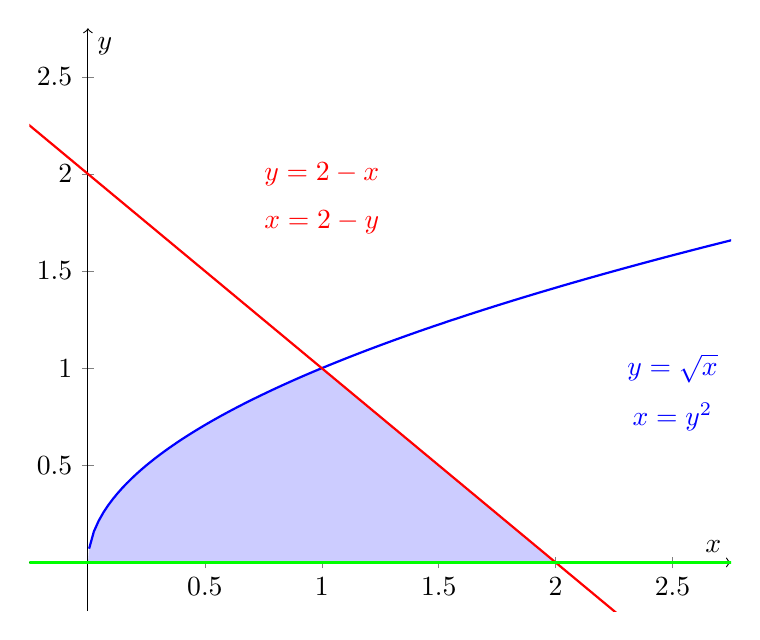
\begin{tikzpicture}
  \begin{axis}[
    axis lines = center,
    xlabel = $x$, ylabel = $y$,
    domain=-1:3,
    samples=200,
    ymin=0, ymax=2.5,
    xmin=0, xmax=2.5,
    enlargelimits=true,
    axis line style={->},
    scale=1.3,
    clip=true,
    ]
    \addplot[blue, thick, name path=A] {x^(1/2)};
    \addplot[red, thick, name path=B] {2-x};
    \addplot[green, thick, name path=C] {0};
    \addplot[blue!20, draw=none] fill between[of=B and C, soft clip={domain=1:2}];
    \addplot[blue!20, draw=none] fill between[of=A and C, soft clip={domain=0:1.01}];

    \node[red] at (1,2) {$y=2-x$};
    \node[red] at (1,1.75) {$x=2-y$};

    \node[blue] at (2.5,1) {$y=\sqrt{x}$};
    \node[blue] at (2.5,0.75) {$x=y^2$};

  \end{axis}
\end{tikzpicture}
\end{center}

\noindent (a)
\begin{align*}V_{\text{Shell}}=\int_0^12\pi y\left[(2-y)-\left(y^2\right)\right]\,dy\end{align*}
\begin{align*}V_{\text{Washer}}=\int_0^1\pi\left[\left(\sqrt x\right)^2-\left(0\right)^2\right]\,dx+\int_1^2\pi\left[\left(2-x\right)^2-\left(0\right)^2\right]\,dx\end{align*}

\hfill

\noindent (b)
\begin{align*}V_{\text{Shell}}=\int_0^12\pi x\left[\left(\sqrt x\right)-(0)\right]\,dx+\int_1^22\pi x\left[\left(2-x\right)-(0)\right]\,dx\end{align*}
\begin{align*}V_{\text{Washer}}=\int_0^1\pi\left[\left(2-y\right)^2-\left(y^2\right)^2\right]\,dy\end{align*}

\noindent 6. If the function $x=f(y)\geq0$ is continuously differentiable on $[a,b]$, the area of the surface generated by revolving the graph of $x=f(y)$ about the $y$-axis is

\[S=\int_a^b2\pi x\sqrt{1+\left(\frac{dx}{dy}\right)^2}\,dy\]

\hfill

\noindent We're interested in the right side of the parabola. So, let $f(y)=\sqrt{y}$ and set $a=1,\:b=4$. Find $\displaystyle\frac{dx}{dy}$ and then calculate the area.

\[\frac{dx}{dy}=\frac1{2\sqrt y}\]

\begin{align*}S&=\int_1^42\pi x\sqrt{1+\left(\frac1{2\sqrt y}\right)^2}\,dy=\int_1^42\pi\sqrt y\cdot\sqrt{1+\frac1{4y}}\,dy=2\pi\int_1^4\sqrt{y+\frac14}\,dy\\\\&=2\pi\left[\frac23\left(y+\frac14\right)^{3/2}\right]_1^4=\frac{4\pi}3\left[\left(\frac{17}4\right)^{3/2}-\left(\frac54\right)^{3/2}\right]=\boxed{\frac\pi6\left(17\sqrt{17}-5\sqrt5\right)}\end{align*}

\hfill

\noindent 7. Let the corresponding function be $\displaystyle f(x)=\frac1{x\ln x^2}$. $f$ is decreasing because $\ln x^2$ and $x$ are increasing for $x\geq2$. These expressions are also continuous for $x\geq2$. $f$ is positive for $x\geq2$. $x=2\implies\ln2^2=\ln4>\ln\mathrm{e}=1>0,\: x=2>0$. Since the conditions are satisfied, we may apply the Integral Test.

\hfill

\noindent Let $u=\ln x^2$, then $\displaystyle du=\frac1{x^2}\cdot 2x\,dx\implies du=\frac2x\,dx$

\[x=2\implies u=\ln2^2=\ln4,\qquad x\to\infty\implies u\to\infty\]

\begin{align*}\int_2^{\infty}\frac1{x\ln x^2}\,dx&=\int_{\ln 4}^{\infty}\frac12\cdot\frac1{u}\,du=\lim_{R\to\infty}\int_{\ln4}^R\frac{du}{2u}=\lim_{R\to\infty}\frac12\ln u\bigg|_{\ln4}^R\\\\&=\frac12\lim_{R\to\infty}\left(\ln R-\ln(\ln 4)\right)=\boxed{\infty}\end{align*}

\hfill

\noindent Since the integral diverges, the series also diverges.

\newpage

\noindent 8. Apply the Ratio Test.

\begin{align*}
\lim_{n\to\infty}\left|\frac{(-1)^{n+1}\cdot(x-2)^{n+1}}{(n+1)\cdot(10)^{n+1}}\cdot\frac{n\cdot(10)^n}{(-1)^n\cdot(x-2)^n}\right|&=\lim_{n\to\infty}\left|-\frac{n(x-2)}{10(n+1)}\right|\\\\&=\frac{|x-2|}{10}\lim_{n\to\infty}\left|\frac n{n+1}\right|=\frac{|x-2|}{10}
\end{align*}

\noindent The series converges absolutely for $\displaystyle \frac{|x-2|}{10}<1$.

\[\frac{|x-2|}{10}<1\implies|x-2|<10\implies-10<x-2<10\implies -8<x<12\]

\hfill

\noindent Investigate the convergence at the endpoints (i.e., $x=-8$ and $x=12$). Try $x=-8$.

\[x=-8\rightarrow\sum_{n=1}^{\infty}(-1)^n\frac1{n\,10^n}(-10)^n=\sum_{n=1}^{\infty}(-1)^n\cdot(-1)^n\cdot\frac1{n}=\sum_{n=1}^{\infty}(-1)^{2n}\cdot\frac1n=\sum_{n=1}^{\infty}\frac1n\]

\hfill

\noindent For $x=-8$, we get a $p$-series where $p=1$. By the $p$-series Test, it diverges. Try $x=12$.

\[x=12\rightarrow\sum_{n=1}^{\infty}(-1)^n\frac1{n\,10^n}(10)^n=\sum_{n=1}^{\infty}\frac{(-1)^n}n\]

\hfill

\noindent This is an alternating series. The non-alternating part, which is $\frac1n$, is nonincreasing for $n\geq2$ and it is positive. The limit at infinity is $0$. By Leibniz's Alternating Series Test, the series converges.

\hfill

\noindent The convergence set for the power series is

\[\boxed{\left(-8,12\right]}\]

\newpage

\begin{center}
2014-2015 Summer Final (23/08/2015) Solutions\\
(Last update: 20/10/2025 23:04)
\end{center}

\noindent 1. $\ln x$ is defined for $x>0$. Therefore, $\ln\left(x^2+1\right)$ is defined on $\mathbb{R}$ because $x^2+1\geq1>0$.

\hfill

\noindent Let us find the limit at infinity and negative infinity.

\begin{equation*}\lim_{x\to\infty}\ln\left(x^2+1\right)=\lim_{x\to-\infty}\ln\left(x^2+1\right)=\infty\end{equation*}

\hfill

\noindent No asymptotes occur.

\hfill

\noindent Take the first derivative and find the critical points. Apply the chain rule.

\[y'=\frac d{dx}\ln\left(x^2+1\right)=\frac1{x^2+1}\cdot 2x=\frac{2x}{x^2+1}\]

\hfill

\noindent A critical point occurs at $x=0$. At this point, the first derivative is $0$.

\hfill

\noindent Take the second derivative. Apply the quotient rule.

\[y''=\frac d{dx}\left(\frac{2x}{x^2+1}\right)=\frac{2\cdot\left(x^2+1\right)-2x\cdot(2x)}{\left(x^2+1\right)^2}=\frac{2-2x^2}{\left(x^2+1\right)^2}\]

\hfill

\noindent The inflection points occur at $x=\pm1$. At these points, the direction of the curvature changes.

\hfill

\noindent Consider some values of the function. Eventually, set up a table and see what the graph looks like in certain intervals.

\begin{equation*}\,f\left(-1\right)=f\left(1\right)=\ln2,\quad f(0)=0\end{equation*}

\begin{center}
    \large
    \begin{tabular}{|c|cccc|} 
    \hline
        $x$&$\left(-\infty,-1\right)$&$\left(-1,0\right)$&$\left(0,1\right)$&$\left(1, \infty\right)$\\
        \hline
        $y$&$(\ln2,\infty)$&$(0,\ln2)$&$(0,\ln2)$&$(\ln2,\infty)$\\
        \hline
        $y'$ sign&-&-&+&+\\
        \hline
        $y''$ sign&-&+&+&-\\
        \hline
    \end{tabular}
\end{center}

\hfill

\begin{center}
\begin{tikzpicture}
  \begin{axis}[
    axis lines = center,
    xlabel = $x$, ylabel = $y$,
    domain=-4:4,
    samples=200,
    ymin=0, ymax=3,
    xmin=-3, xmax=3,
    restrict y to domain=-5:5,
    enlargelimits=true,
    axis line style={->},
    scale=1.4,
    ]
    \addplot[blue, thick] {ln(x^2+1)};
    \draw[dashed](-1,0)--(-1,0.693);\draw[dashed](1,0)--(1,0.693);\draw[dashed](-1,0.693)--(0,0.693);\draw[dashed](0,0.693)--(1,0.693);
    \node at (-0.2,0.77) {\small$\ln2$};
  \end{axis}
\end{tikzpicture}
\end{center}

\newpage

\noindent 2.
\begin{center}
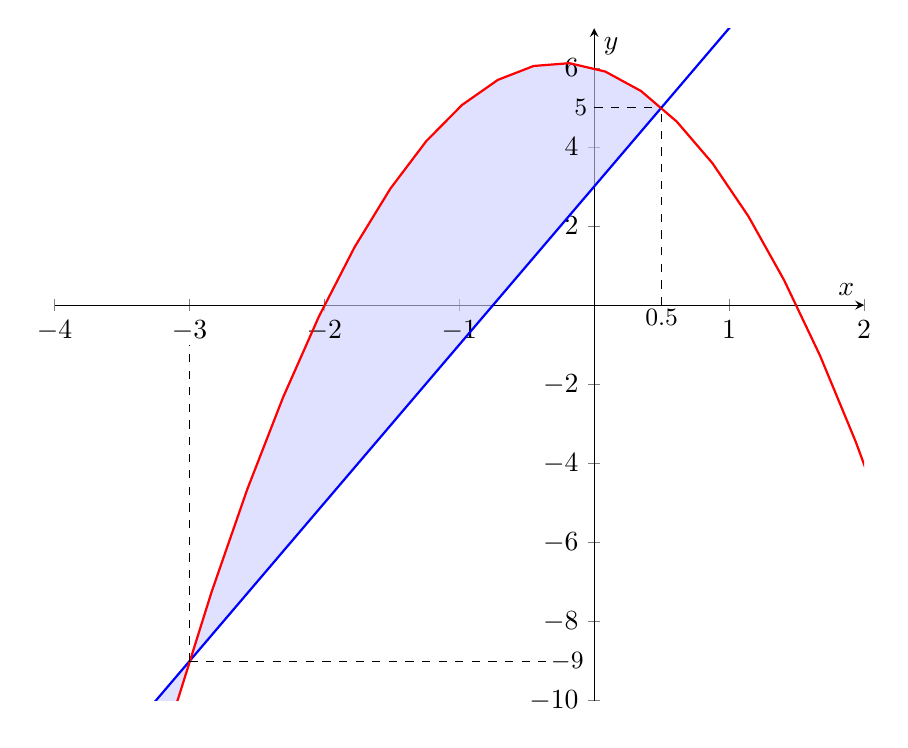
\begin{tikzpicture}
  \begin{axis}[
      axis lines=center,
      xlabel={$x$},
      ylabel={$y$},
      xmin=-4, xmax=2,
      ymin=-10, ymax=7,
      samples=50,
      clip=true,
      scale=1.5,
      domain=-10:3,
    ]

    \addplot [thick, blue, name path=A] {4*x+3};
    \addplot [thick, red, domain=-10:3, name path=B] {6-x-2*x^2};
    \addplot [blue!20, fill opacity=0.6] fill between[of=A and B,soft clip={domain=-9:0.5}];
    
    \draw[dashed] (-3,-9) -- (-3,-1); \draw[dashed] (-3,-9) -- (-0.3,-9);
    \draw[dashed] (0.5,0) -- (0.5,5); \draw[dashed] (0,5) -- (0.5,5);

    \node at (axis cs:-0.1,5) {\small $5$};
    \node at (axis cs:-0.2,-9) {\small $-9$};
    \node at (axis cs:0.5,-0.3) {\small $0.5$};
  \end{axis}
\end{tikzpicture}
\end{center}
\begin{align*}
\text{Area}&=\int_{-3}^{1/2}\left[6-x-2x^2-(4x+3)\right]\,dx=\int_{-3}^{1/2}\left(3-5x-2x^2\right)\,dx\\\\&=3x-\frac{5x^2}2-\frac{2x^3}3\Bigg|_{-3}^{1/2}=\left(\frac32-\frac58-\frac1{12}\right)-\left(-9-\frac{45}2+18\right)=\boxed{\frac{343}{24}}
\end{align*}

\hfill

\noindent 3.
\begin{center}
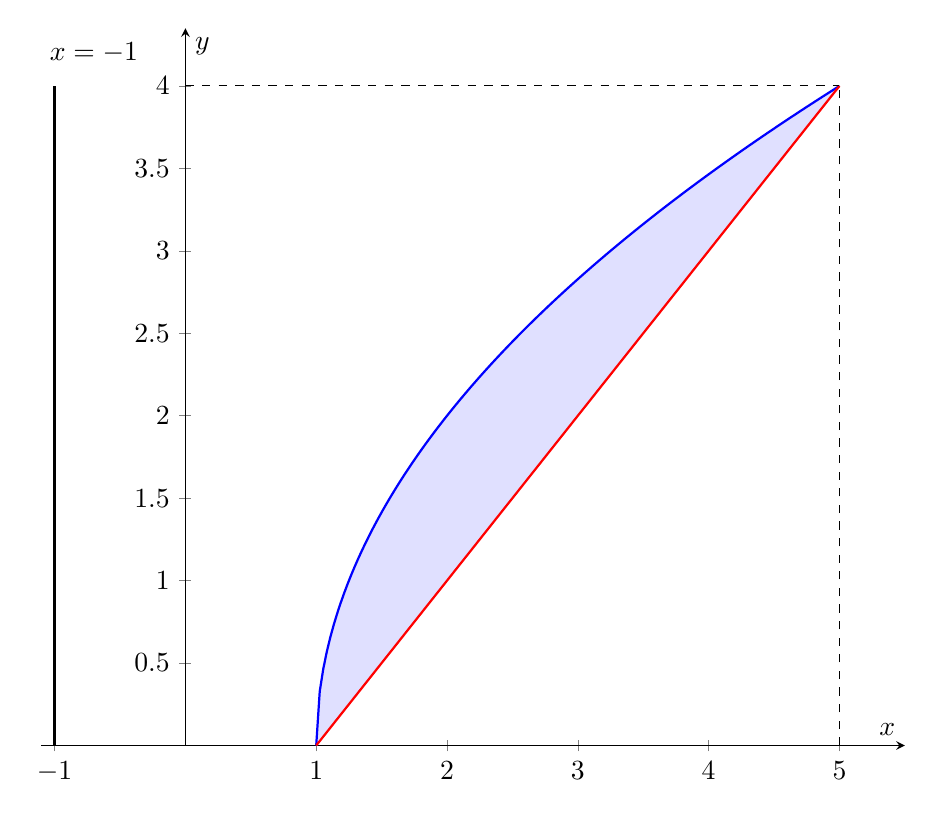
\begin{tikzpicture}
  \begin{axis}[
      axis lines=center,
      xlabel={$x$},
      ylabel={$y$},
      xmin=-1.1, xmax=5.5,
      ymin=0, ymax=4.35,
      samples=150,
      clip=true,
      scale=1.6,
      domain=1:5,
    ]

    \addplot [thick, blue, name path=A] {2*sqrt(x-1)};
    \addplot [thick, red, name path=B] {x-1};
    \addplot [blue!20, fill opacity=0.6] fill between[of=A and B,soft clip={domain=1:5}];
    
    \draw[dashed] (5,0) -- (5,4); \draw[thick] (-1,0) -- (-1,4); \draw[dashed] (0,4) -- (5,4);
    \node at (-0.7,4.2) {$x=-1$};
  \end{axis}
\end{tikzpicture}
\end{center}

\noindent Rewrite the equations of the curves and solve for $x$. Let $V$ be the volume of the solid.

\[y=2\sqrt{x-1}\implies y^2=4x-4\implies x=\frac{y^2+4}4\]
\[y=x-1\implies x=y+1\]

\begin{align*}
V&=\int_D\pi\left[R_2^2(y)-R_1^2(y)\right]\,dy=\int_0^4\pi\left[\left((y+1)+1\right)^2-\left(\left(\frac{y^2+4}4\right)+1\right)^2\right]\,dy\\\\&=\pi\int_0^4\left[(y+2)^2-\left(\frac{y^2}4+2\right)^2\right]\,dy=\pi\int_0^4\left(y^2+4y+4-\frac{y^4}{16}-y^2-4\right)\,dy\\\\&=\pi\int_0^4\left(4y-\frac{y^4}{16}\right)\,dy=\pi\left[2y^2-\frac{y^5}{80}\right]_0^4=\pi\left[\left(32-\frac{64}{5}\right)-\left(0\right)\right]=\boxed{\frac{96\pi}5}
\end{align*}

\hfill

\noindent 4.
\begin{center}
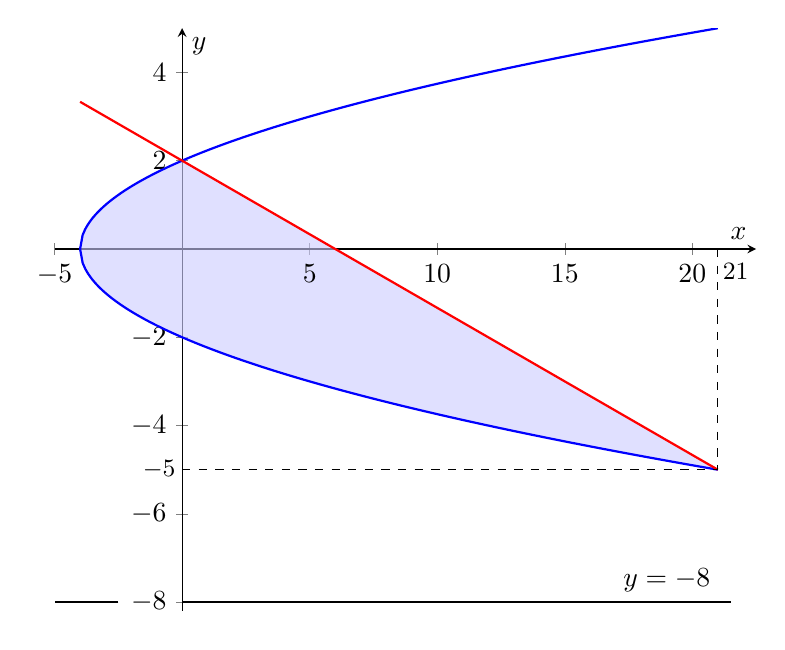
\begin{tikzpicture}
  \begin{axis}[
      axis lines=center,
      xlabel={$x$},
      ylabel={$y$},
      xmin=-5, xmax=22.5,
      ymin=-8.2, ymax=5,
      samples=250,
      clip=true,
      scale=1.3,
      domain=-4:21,
    ]

    \addplot [thick, blue, name path=A] {sqrt(x+4)};
    \addplot [thick, blue, name path=B] {-sqrt(x+4)};
    \addplot [thick, red, name path=C] {(6-x)/3};
    \addplot [blue!20, fill opacity=0.6] fill between[of=A and B,soft clip={domain=-4:0}];
    \addplot [blue!20, fill opacity=0.6] fill between[of=C and B,soft clip={domain=0:21}];

    \draw[dashed] (21,0)--(21,-5); \draw[thick] (0,-8)--(21.5,-8); \draw[thick] (-2.5,-8)--(-5,-8); \draw[dashed] (0,-5)--(21,-5);
    \node at (19,-7.5) {$y=-8$};
    \node at (21.7,-0.5) {\small $21$};
    \node at (-0.9,-5) {\small $-5$};
  \end{axis}
\end{tikzpicture}
\end{center}

\noindent Let $V$ be the volume of the solid.

\begin{align*}
V&=\int_D2\pi\cdot h(y)\cdot r(y)\,dy=2\pi\int_{-5}^2(y+8)\cdot\left[(6-3y)-(y^2-4)\right]\,dy\\\\&=2\pi\int_{-5}^2(y+8)(-y^2-3y+10)\,dy=2\pi\int_{-5}^2\left(-y^3-3y^2+10y-8y^2-24y+80\right)\,dy\\\\&=2\pi\int_{-5}^2\left(-y^3-11y^2-14y+80\right)\,dy=2\pi\left[-\frac{y^4}4-\frac{11y^3}3-7y^2+80y\right]_{-5}^2\\\\&=2\pi\left[\left(-4-\frac{88}3-28+160\right)-\left(\frac{625}4+\frac{1375}3-175-400\right)\right]=\boxed{\frac{4459\pi}6}
\end{align*}

\newpage

\noindent 5.

\hfill

\noindent (a) Use the $u$-substitution method. Let $u=\mathrm{e}^{-x}+\ln x$. Then $\displaystyle du=\left(-\mathrm{e}^{-x}+\frac1x\right)\,dx$.

\begin{align*}\int4\left(\frac1x-\mathrm{e}^{-x}\right)\cos\left(\mathrm{e}^{-x}+\ln x\right)\,dx&=\int4\cos u\,du=4\sin u+c\\\\&=\boxed{4\sin\left(\mathrm{e}^{-x}+\ln x\right)+c,\:c\in\mathbb{R}}\end{align*}

\hfill

\noindent (b) Decompose the fraction into multiple partial fractions. Let $A,\:B,\:C,\:D,\:E,\:F\in\mathbb{R}$.

\begin{align*}\mathrm{I}=\int\frac{x^3+10x^2+3x+36}{(x-1)^2\,\left(x^2+4\right)^2}\,dx=\int\left(\frac{A}{x-1}+\frac{B}{(x-1)^2}+\frac{Cx+D}{x^2+4}+\frac{Ex+F}{(x^2+4)^2}\right)\,dx\end{align*}

\hfill

\noindent Let $N=x^3+10x^2+3x+36$.

\begin{align*}
N&=A\left(x^2+4\right)^2(x-1)+B\left(x^2+4\right)^2+(Cx+D)\left(x^2+4\right)(x-1)^2+(Ex+F)(x-1)^2\\\\&=\left(x^2+4\right)^2\left[A(x-1)+B\right]+(x-1)^2\left[(Cx+D)\left(x^2+4\right)+Ex+F\right]\\\\&=\left(x^4+8x^2+16\right)(Ax-A+B)+\left(x^2-2x+1\right)\\&\hspace{1em}\cdot\left(Cx^3+4Cx+Dx^2+4D+Ex+F\right)\\\\&=Ax^5-Ax^4+Bx^4+8Ax^3-8Ax^2+8Bx^2+16Ax-16A+16B\\&\hspace{1em}+Cx^5+4Cx^3+Dx^4+4Dx^2+Ex^3+Fx^2-2Cx^4-8Cx^2-2Dx^3-8Dx\\&\hspace{1em}-2Ex^2-2Fx+Cx^3+4Cx+Dx^2+4D+Ex+F\\\\&=x^5\left(A+C\right)+x^4\left(-A+B+D-2C\right)+x^3\left(8A+4C+E-2D+C\right)\\&\hspace{1em}+x^2\left(-8A+8B+4D+F-8C-2E+D\right)+x\left(16A-8D-2F+4C+E\right)\\&\hspace{1em}-16A+16B+4D+F
\end{align*}

\hfill

\noindent Equate the coefficients of like terms.

\begin{align}
A+C&=0\\
-A+B+D-2C&=0\nonumber\\
8A+5C+E-2D&=1\nonumber\\
-8A+8B+5D-8C+F-2E&=10\nonumber\\
16A-8D-2F+4C+E&=3\nonumber\\
-16A+16B+4D+F&=36\nonumber
\end{align}

\noindent From $(1)$, $A=-C$. Rewrite $C$ in terms of $A$ and rearrange the equations.

\begin{align}
A+B+D&=0\\
3A+E-2D&=1\nonumber\\
8B+5D+F-2E&=10\nonumber\\
12A-8D-2F+E&=3\nonumber\\
-16A+16B+4D+F&=36\nonumber
\end{align}

\noindent From $(2)$, $A+B=-D$. Rewrite $D$ in terms of $A$ and $B$ and rearrange the equations.

\begin{align}
5A+2B+E&=1\\
-5A+3B+F-2E&=10\\
20A+8B-2F+E&=3\\
-20A+12B+F&=36
\end{align}

\noindent By using the couples $(3)\And(4)$ and $(4)\And(5)$, eliminate $E$.

\[\left.\begin{array}{rl}
5A+7B+F&=12\\
35A+19B-3F&=16\\
-20A+12B+F&=36
\end{array}\right\}\quad\implies\left.\begin{array}{rl}
50A+40B&=52\\
-25A+55B&=124
\end{array}\right\}\implies A=-\frac{14}{25},\:B=2
\]

\hfill

\noindent Therefore, $\displaystyle C=\frac{14}{25},\:D=-\frac{36}{25}$. From $(3)$, $\displaystyle E=-\frac15$, and from $(6)$, $\displaystyle F=\frac45$.

\hfill

\noindent Substitute the values into $A,\:B,\:C,\:D,\:E,\:F$.

\begin{equation}\mathrm{I}=\int\left(-\frac{14}{25}\cdot\frac1{x-1}+\frac2{(x-1)^2}+\frac{\frac{14}{25}x-\frac{36}{25}}{x^2+4}+\frac{-\frac15x+\frac45}{\left(x^2+4\right)^2}\right)\,dx\end{equation}

\hfill

\noindent From now on, integrate term by term. Integrate the first term in $(7)$.

\hfill

\begin{equation}\int-\frac{14}{25}\cdot\frac1{x-1}\,dx=-\frac{14}{25}\int\frac1{x-1}\,dx=-\frac{14}{25}\ln\left|x-1\right|+c\end{equation}

\hfill

\noindent Integrate the second term in $(7)$.

\hfill

\begin{equation}\int\frac{2}{(x-1)^2}\,dx=-\frac2{x-1}+c\end{equation}

\hfill

\noindent Integrate the third term in $(7)$.

\begin{align}\int\frac{\frac{14}{25}x-\frac{36}{25}}{x^2+4}\,dx&=\frac1{25}\int\frac{14x-36}{x^2+4}\,dx=\frac{7}{25}\int\frac{2x}{x^2+4}\,dx-\frac{36}{25}\int\frac1{x^2+4}\,dx\nonumber\\\nonumber\\&=\frac7{25}\ln\left|x^2+4\right|-\frac{36}{100}\int\frac1{\left(\frac x2\right)^2+1}\,dx\nonumber\\\nonumber\\&=\frac7{25}\ln\left(x^2+4\right)-\frac{36}{50}\arctan\left(\frac x2\right)+c\end{align}

\newpage

\noindent Integrate the last term in $(7)$.

\begin{align}\int\frac{-\frac15x+\frac45}{\left(x^2+4\right)^2}\,dx&=\frac15\int\frac{4-x}{\left(x^2+4\right)^2}\,dx=\frac45\int\frac1{\left(x^2+4\right)^2}\,dx-\frac15\int\frac x{\left(x^2+4\right)^2}\,dx\end{align}

\hfill

\noindent First, solve the integral on the left in $(11)$. Let $x=2\tan u$, then $dx=2\sec^2u\,du$.

\begin{align*}\int\frac1{\left(x^2+4\right)^2}\,dx&=\int\frac{2\sec^2u}{\left(4\tan^2u+4\right)^2}du=\int\frac{2\sec^2u}{16\sec^4u}\,du=\frac18\int\frac1{\sec^2u}\,du\\\\&=\frac18\int\cos^2u\,du=\frac18\int\left(\frac{1-\cos2u}2\right)\,du=\frac18\left(\frac u2-\frac{\sin2u}4\right)+c\\\\&=\frac u{16}-\frac{\sin u\cos u}{16}+c\end{align*}

\hfill

\noindent Since $x=2\tan u$, $\displaystyle\tan u=\frac x2$

\[u=\arctan \frac x2,\quad \sin u=\frac x{\sqrt{x^2+4}},\quad\cos u=\frac 2{\sqrt{x^2+4}}\]

\hfill

\noindent Rewrite the integral.

\begin{equation}\int\frac1{\left(x^2+4\right)^2}\,dx=\frac1{16}\left(\arctan \frac x2-\frac {2x}{x^2+4}\right)+c\end{equation}

\hfill

\noindent Now, solve the integral on the right in $(11)$. Let $u=x^2+4$, then $du=2x\,dx$.

\begin{equation}\int\frac x{\left(x^2+4\right)^2}\,dx=\int\frac{du}{2u^2}=-\frac1{2u}+c=-\frac1{2\left(x^2+4\right)}+c\end{equation}

\hfill

\noindent Rewrite the integral in $(11)$ using $(12)$ and $(13)$.

\begin{equation}\frac45\int\frac1{\left(x^2+4\right)^2}\,dx-\frac15\int\frac x{\left(x^2+4\right)^2}\,dx=\frac1{20}\left(\arctan\frac x2+\frac{2x+2}{x^2+4}\right)+c\end{equation}

\hfill

\noindent Eventually, using $(8),\:(9),\:(10)$ and $(14)$, rewrite $(7)$.

\[\mathrm{I}=\boxed{-\frac{14}{25}\ln\left|x-1\right|-\frac2{x-1}+\frac7{25}\ln\left(x^2+4\right)-\frac{67}{100}\arctan\frac x2+\frac{x+1}{10\left(x^2+4\right)}+c,\ c\in\mathbb{R}}\]

\hfill

\noindent (c) Let $\displaystyle x=\frac25\sec u$ for $\displaystyle 0\leq u<\frac\pi2$, then $dx=\displaystyle\frac25\sec u\tan u\,du$.

\[\mathrm{I}=\int\frac{\sqrt{25x^2-4}}{x}\,dx=\int\frac{\sqrt{4\sec^2u-4}}{\frac25\sec u}\cdot\frac25\sec u\tan u\,du\qquad\left[\tan^2u+1=\sec^2u\right]\]

\newpage

\begin{align*}\mathrm{I}&=2\int\left|\tan u\right|\tan u\,du\qquad\left[\tan u>0\right]\\\\&=2\int\tan^2u\,du=2\int\sec^2u\,du-2\int\,du=2\tan u-2u+c\end{align*}

\noindent Recall that $\displaystyle x=\frac25\sec u$.

\[\sec u=\frac{5x}2\implies\sec^2u=\frac{25x^2}4\implies\tan u=\frac{\sqrt{25x^2-4}}2\implies u=\arctan\left(\frac{\sqrt{25x^2-4}}2\right)\]

\[\int\frac{\sqrt{25x^2-4}}{x}\,dx=\boxed{\sqrt{25x^2-4}-2\arctan\left(\frac{\sqrt{25x^2-4}}2\right)+c,\quad c\in\mathbb{R}}\]

\hfill

\noindent (d) Use the method of integration by parts.

\[
\left.\begin{array}{c}
u=x^2\implies du=2x\,dx\\[1em]
\displaystyle dv=\cos(4x)\,dx\implies v=\frac14\sin(4x)
\end{array}\right\}\rightarrow\int u\,dv=uv-\int v\,du
\]

\[\mathrm{I}=x^2\cdot\frac14\sin(4x)-\int\frac14\sin(4x)\cdot2x\,dx=\frac{x^2}4\sin(4x)-\frac12\int x\sin(4x)\,dx\]

\hfill

\noindent Apply the same procedure.

\[
\left.\begin{array}{c}
w=x\implies dw=dx\\[1em]
\displaystyle dz=\sin(4x)\,dx\implies z=-\frac14\cos(4x)
\end{array}\right\}\rightarrow\int w\,dz=wz-\int z\,dw
\]
\begin{align*}\mathrm{I}&=\frac{x^2}4\sin(4x)-\frac12\left[\frac{-x}4\cos(4x)-\int-\frac14\cos(4x)\,dx\right]\\\\&=\boxed{\frac{x^2}4\sin(4x)+\frac x8\cos(4x)-\frac1{32}\sin(4x)+c,\quad c\in\mathbb{R}}\end{align*}

\hfill

\noindent (e)
\begin{align*}\int\frac{dx}{2x^2-3x+2}&=\int\frac{dx}{\displaystyle2x^2-3x+\frac98+\frac78}=\int\frac{dx}{\displaystyle\left(\sqrt2x-\frac{3\sqrt2}4\right)^2+\frac78}\\\\&=\frac87\int\frac{dx}{\displaystyle\frac{8\left(\sqrt2x-\frac{3\sqrt2}4\right)^2}7+1}\end{align*}

\hfill

\noindent Let $\displaystyle u=\frac{2\sqrt2}{\sqrt7}\left(\sqrt2x-\frac{3\sqrt2}4\right)$, then $\displaystyle du=\frac4{\sqrt7}\,dx$.

\begin{align*}\frac87\int\frac{dx}{\displaystyle\frac{8\left(\sqrt2x-\frac{3\sqrt2}4\right)^2}7+1^2}&=\frac87\int\frac{1}{u^2+1}\cdot\frac{\sqrt7}4\,du=\frac2{\sqrt7}\int\frac1{u^2+1}\,du=\frac2{\sqrt7}\arctan u+c\\&=\frac2{\sqrt7}\arctan\left[\frac{2\sqrt2}{\sqrt7}\left(\sqrt2x-\frac{3\sqrt2}4\right)\right]+c,\quad c\in\mathbb{R}\\\\&=\boxed{\frac2{\sqrt7}\arctan\left(\frac{4x-3}{\sqrt7}\right)+c,\quad c\in\mathbb{R}}\end{align*}

\hfill

\noindent 6. Use the method of integration by parts.

\[
\left.\begin{array}{c}
u=1+2x\implies du=2\,dx\\
dv=\mathrm{e}^{-x}\,dx\implies v=-\mathrm{e}^{-x}
\end{array}\right\}\rightarrow\int u\,dv=uv-\int v\,du
\]

\begin{align*}\int_{-\infty}^0(1+2x)\,\mathrm{e}^{-x}\,dx&=\lim_{R\to-\infty}-\mathrm{e}^{-x}(1+2x)\bigg|_R^0-\int_{-\infty}^0-\mathrm{e}^{-x}\cdot2\,dx\\\\&=\lim_{R\to-\infty}\left(-\mathrm{e}^0\cdot1+\mathrm{}e^{-R}(1+2\cdot R)\right)+\lim_{P\to-\infty}2\mathrm{e}^{-x}\bigg|_P^0\\\\&=-\infty+2\lim_{P\to-\infty}\left(\mathrm{e}^0-\mathrm{e}^{-P}\right)=-\infty-\infty=\boxed{-\infty}\end{align*}

\hfill

\noindent The integral diverges to negative infinity.

\hfill

\noindent 7. The length of a curve defined by $x=f(y)$ whose derivative is continuous on the interval $a\leq y\leq b$ can be evaluated using the integral

\[S=\int_a^b\sqrt{1+\left(\frac{dx}{dy}\right)^2}\,dy.\]

\hfill

\noindent Find $\displaystyle\frac{dx}{dy}$.

\[\frac{dx}{dy}=\frac23\cdot\frac32(y-1)^{1/2}=\sqrt{y-1}\]

\hfill

\noindent Set $a=1,\:b=2$ and find the length.

\[S=\int_1^2\sqrt{1+\left(\sqrt{y-1}\right)^2}\,dy=\int_1^2\sqrt{y}\,dy=\frac23y^{3/2}\,\bigg|_1^2=\boxed{\frac23(2\sqrt2-1)}\]

\newpage

\begin{center}
2015-2016 Final (12/01/2016) Solutions\\
(Last update: 30/08/2025 00:48)
\end{center}

\noindent 1.
\begin{center}
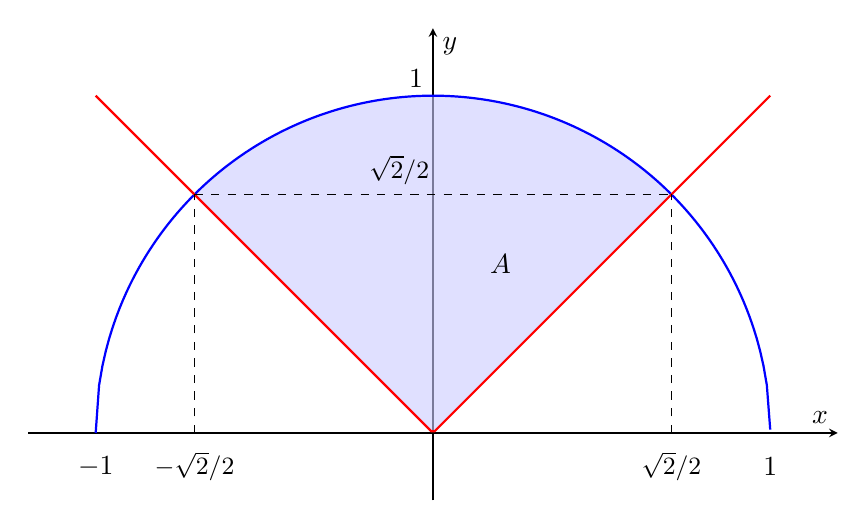
\begin{tikzpicture}
  \begin{axis}[
      axis lines=center,
      axis equal image,
      xlabel={$x$},
      ylabel={$y$},
      xtick=\empty, ytick=\empty,
      xmin=-1.2, xmax=1.2,
      ymin=-0.2, ymax=1.2,
      samples=200,
      scale=1.5,
      domain=-1:1,
    ]

    \addplot [thick, blue, name path=A, domain=-1:1] {sqrt(1-x^2)};
    \addplot [thick, red, name path=B] {abs(x)};
    \addplot [blue!20, fill opacity=0.6] fill between[of=A and B,soft clip={domain=-0.707:0.707}];
    
    \draw[dashed] (-0.707,0) -- (-0.707,0.707);
    \draw[dashed] (0.707,0) -- (0.707,0.707);
    \draw[dashed] (-0.707,0.707) -- (0.707,0.707);

    \node at (axis cs:0.707,-0.1) {\small $\sqrt2/2$};
    \node at (axis cs:-0.707,-0.1) {\small $-\sqrt2/2$};
    \node at (axis cs:-0.1,0.78) {\small $\sqrt2/2$};
    \node at (axis cs:-1,-0.1) {$-1$};
    \node at (axis cs:1,-0.1) {$1$};
    \node at (axis cs:-0.05,1.05) {$1$};
    \node at (0.2,0.5) {$A$};
\end{axis}
\end{tikzpicture}
\end{center}
\begin{align}
A&=\int_{-\sqrt2/2}^{\sqrt2/2}\left(\sqrt{1-x^2}-\left|x\right|\right)\,dx=\int_{-\sqrt2/2}^0\left(\sqrt{1-x^2}+x\right)\,dx+\int_0^{\sqrt2/2}\left(\sqrt{1-x^2}-x\right)\,dx\nonumber\\\nonumber\\&=\int_{-\sqrt2/2}^{\sqrt2/2}\sqrt{1-x^2}\,dx-\int_0^{\sqrt2/2}2x\,dx
\end{align}

\hfill

\noindent Calculate the right-hand integral $(1)$.

\[\int_0^{\sqrt2/2}2x\,dx=x^2\bigg|_0^{\sqrt2/2}=\left(\frac{\sqrt2}2\right)^2-\left(0\right)^2=\frac12\]

\hfill

\noindent To calculate the left-hand integral in $(1)$, we will use a trigonometric substitution. Let $x=\sin u$, then $dx=\cos u\,du$.

\[x=-\frac{\sqrt2}2\implies u=\arcsin\left(-\frac{\sqrt2}2\right)=-\frac{\pi}4,\qquad x=\frac{\sqrt2}2\implies u=\arcsin\left(\frac{\sqrt2}2\right)=\frac{\pi}4\]

\begin{align*}\int_{-\sqrt2/2}^{\sqrt2/2}\sqrt{1-x^2}\,dx&=\int_{-\pi/4}^{\pi/4}\sqrt{1-\sin^2u}\cos u\,du=\int_{-\pi/4}^{\pi/4}\left|\cos u\right|\cos u\,du\quad\left[\left|\cos u\right|>0\right]\\\\&=\int_{-\pi/4}^{\pi/4}\cos^2u\,du=\int_{-\pi/4}^{\pi/4}\frac{1+\cos2u}{2}\,du=\left[\frac u2+\frac{\sin2u}4\right]_{-\pi/4}^{\pi/4}\\\\&=\left(\frac\pi8+\frac14\right)-\left(-\frac\pi8-\frac14\right)=\frac\pi4-\frac12\end{align*}

\hfill

\noindent Evaluate $(1)$. The area is $\displaystyle A=\left(\frac\pi4+\frac12\right)-\left(\frac12\right)=\boxed{\frac\pi4}$.

\newpage

\noindent 2.
\begin{center}
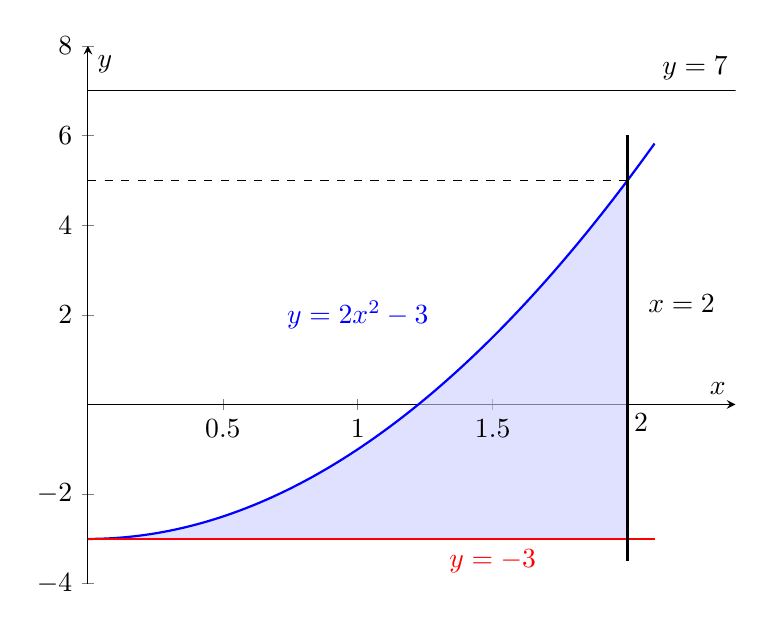
\begin{tikzpicture}
  \begin{axis}[
      axis lines=center,
      xlabel={$x$},
      ylabel={$y$},
      xmin=0, xmax=2.4,
      ymin=-4, ymax=8,
      samples=150,
      xticklabels={,,$0.5$,$1$,$1.5$,},
      clip=true,
      scale=1.2,
      domain=0:2.1,
    ]

    \addplot [thick, blue, name path=A] {2*x^2-3};
    \addplot [thick, red, name path=B] {-3};
    \addplot [blue!20, fill opacity=0.6] fill between[of=A and B,soft clip={domain=0:2}];
    \draw (0,7)--(5,7); \draw[thick] (2,-3.5)--(2,6); \draw[dashed] (0,5)--(2,5);
    \node at (2.25,7.5) {$y=7$};
    \node[blue] at (1,2) {$y=2x^2-3$};
    \node at (2.2,2.25) {$x=2$};
    \node[red] at (1.5,-3.5) {$y=-3$};
    \node at (2.05,-0.4) {$2$};
  \end{axis}
\end{tikzpicture}
\end{center}
\begin{align*}
V&=\int_D\pi\left[R_2^2(x)-R_1^2(x)\right]\,dx=\int_0^2\pi\left[\left(7-(-3)\right)^2-\left(7-\left(2x^2-3\right)\right)^2\right]\,dx\\\\&=\pi\int_0^2\left[(10)^2-\left(10-2x^2\right)^2\right]\,dx=\pi\int_0^2\left(100-100+40x^2-4x^4\right)\,dx\\\\&=\pi\int_0^2\left(40x^2-4x^4\right)\,dx=\pi\left[\frac{40x^3}3-\frac{4x^5}5\right]_0^2=\pi\left[\left(\frac{320}3-\frac{128}5\right)-\left(0\right)\right]=\boxed{\frac{1216\pi}{15}}
\end{align*}

\hfill

\noindent 3.
\begin{center}
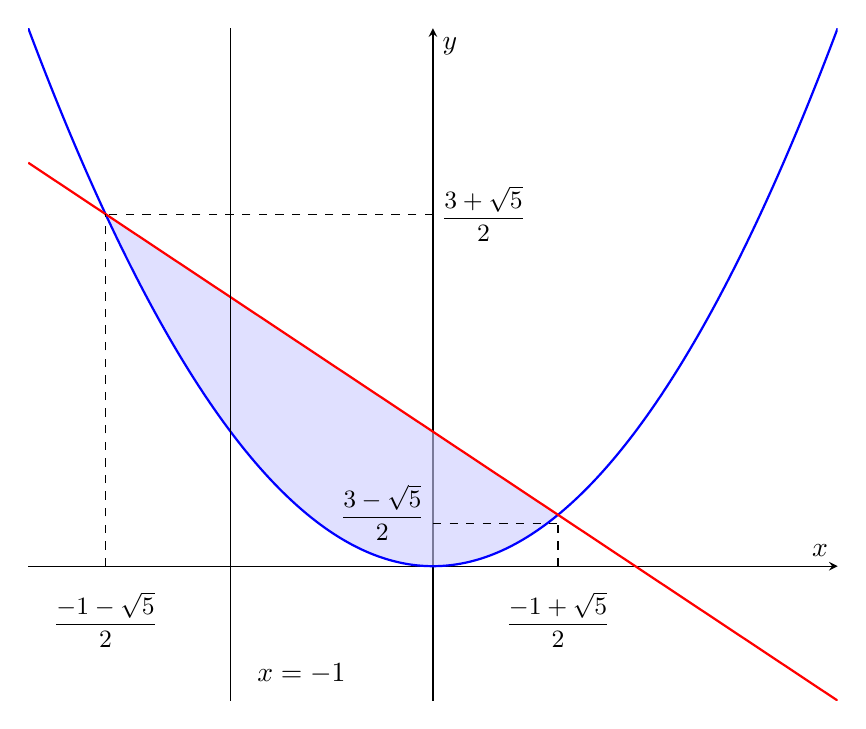
\begin{tikzpicture}
  \begin{axis}[
      axis lines=center,
      xlabel={$x$},
      ylabel={$y$},
      ytick=\empty, xtick=\empty,
      xmin=-2, xmax=2,
      ymin=-1, ymax=4,
      samples=250,
      clip=true,
      scale=1.5,
      domain=-2:2,
    ]

    \addplot [thick, blue, name path=A] {x^2};
    \addplot [thick, red, name path=B] {-x+1};
    \addplot [blue!20, fill opacity=0.6] fill between[of=A and B, soft clip={domain=-1.618:0.618}];
    
    \node at (-1.618,-0.4) {\small $\displaystyle\frac{-1-\sqrt5}2$};
    \node at (0.618,-0.4) {\small $\displaystyle\frac{-1+\sqrt5}2$};
    \node at (0.25,2.618) {\small $\displaystyle\frac{3+\sqrt5}2$};
    \node at (-0.25,0.4) {\small $\displaystyle\frac{3-\sqrt5}2$};
    \node at (-0.65,-0.8) {$x=-1$};
    
    \draw[dashed] (-1.618,0)--(-1.618,2.618); \draw[dashed] (0,2.618)--(-1.618,2.618);
    \draw[dashed] (0.618,0)--(0.618,0.318); \draw[dashed] (0,0.318)--(0.618,0.318);
    \draw (-1,-1)--(-1,4);
  \end{axis}
\end{tikzpicture}
\end{center}

\noindent Notice that the rotation axis passes through the region. Consider the right-hand region. If we rotate it around the axis, a piece of the region on the left will be inside the revolution. That is, the region bounded by the line that is symmetric to the line $y=-x+1$ around $x=-1$ and the curve $y=x^2$. We do not need to rotate that region since it would lead to double revolution. The upper part of the left-hand region may be rotated around $x=-1$ independent of the right-hand region. Divide the left-hand region into three subregions. We get three different subregions to integrate over.

\begin{center}
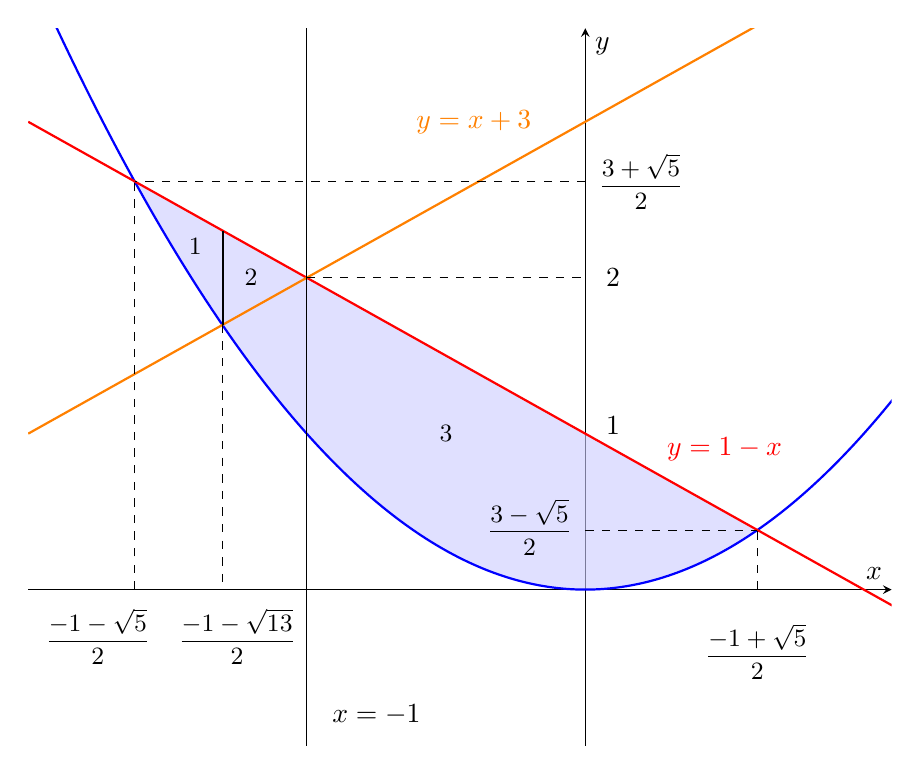
\begin{tikzpicture}
  \begin{axis}[
      axis lines=center,
      xlabel={$x$},
      ylabel={$y$},
      ytick=\empty, xtick=\empty,
      xmin=-2, xmax=1.1,
      ymin=-1, ymax=3.6,
      samples=250,
      clip=true,
      scale=1.6,
      domain=-2:2,
    ]

    \addplot [thick, blue, name path=A] {x^2};
    \addplot [thick, red, name path=B] {-x+1};
    \addplot [thick, orange] {x+3};
    \addplot [blue!20, fill opacity=0.6] fill between[of=A and B, soft clip={domain=-1.618:0.618}];
    
    \node at (-1.75,-0.3) {\small $\displaystyle\frac{-1-\sqrt5}2$};
    \node at (-1.25,-0.3) {\small $\displaystyle\frac{-1-\sqrt{13}}2$};
    \node at (0.618,-0.4) {\small $\displaystyle\frac{-1+\sqrt5}2$};
    \node at (0.2,2.618) {\small $\displaystyle\frac{3+\sqrt5}2$};
    \node at (-0.2,0.4) {\small $\displaystyle\frac{3-\sqrt5}2$};
    \node at (-0.75,-0.8) {$x=-1$};
    \node[orange] at (-0.4,3) {$y=x+3$};
    \node[red] at (0.5,0.9) {$y=1-x$};
    \node at (0.1,2) {$2$};
    \node at (0.1,1.05) {$1$};

    \draw[dashed] (-1.618,0)--(-1.618,2.618); \draw[dashed] (0,2.618)--(-1.618,2.618);
    \draw[dashed] (0.618,0)--(0.618,0.381); \draw[dashed] (0,0.381)--(0.618,0.381);
    \draw[thick] (-1.302, 1.698)--(-1.302,2.302);
    \draw[dashed] (-1.302, 1.698)--(-1.302,0);
    \draw[dashed] (-1,2)--(0,2);

    \node at (-1.4,2.2) {\small $1$};
    \node at (-1.2,2) {\small $2$};
    \node at (-0.5,1) {\small $3$};

    \draw (-1,-1)--(-1,4);
  \end{axis}
\end{tikzpicture}
\end{center}

\noindent Let $V$ be the volume of the solid.

\begin{align*}V&=\int_D2\pi\cdot r(x)\cdot h(x)\,dx\\\\&=\int_{\textstyle\frac{-1-\sqrt5}2}^{\textstyle\frac{1-\sqrt{13}}2}2\pi(-1-x)\left[\left(1-x\right)-x^2\right]\,dx+\int_{\textstyle\frac{1-\sqrt{13}}2}^{-1}2\pi(-1-x)\left[\left(1-x\right)-\left(x+3\right)\right]\,dx\\\\&\quad\:+\int_{-1}^{\textstyle\frac{-1+\sqrt5}2}2\pi\left(x+1\right)\left[\left(1-x\right)-x^2\right]\,dx\\\\&=2\pi\int_{\textstyle\frac{-1-\sqrt5}2}^{\textstyle\frac{1-\sqrt{13}}2}\left(-1+2x^2+x^3\right)\,dx+2\pi\int_{\textstyle\frac{1-\sqrt{13}}2}^{-1}\left(2x^2+4x+2\right)\,dx\\\\&\quad\:+2\pi\int_{-1}^{\textstyle\frac{-1+\sqrt5}2}\left(1-2x^2-x^3\right)\,dx\\\\&=2\pi\left\{\left[-x+\frac{2x^3}3+\frac{x^4}4\right]_{\textstyle\frac{-1-\sqrt5}2}^{\textstyle\frac{1-\sqrt{13}}2}+\left[\frac{2x^3}3+2x^2+2x\right]_{\textstyle\frac{1-\sqrt{13}}2}^{-1}+\left[x-\frac{2x^3}3-\frac{x^4}4\right]_{-1}^{\textstyle\frac{-1+\sqrt5}2}\right\}\end{align*}

\newpage

\begin{align*}V&=2\pi\left[\frac{\sqrt{13}-1}2+\frac{\left(1-\sqrt{13}\right)^3}{12}+\frac{\left(1-\sqrt{13}\right)^4}{64}-\frac{1+\sqrt5}2+\frac{\left(1+\sqrt5\right)^3}{12}-\frac{\left(1+\sqrt5\right)^4}{64}\right]\\\\&\quad\:+2\pi\left[-\frac23+2-2-\left(\frac{\left(1-\sqrt{13}\right)^3}{12}+\frac{\left(1-\sqrt{13}\right)^2}2+1-\sqrt{13}\right)\right]\\\\&\quad\:+2\pi\left[\frac{-1+\sqrt5}2-\frac{\left(-1+\sqrt5\right)^3}{12}-\frac{\left(-1+\sqrt5\right)^4}{64}-\left(-1+\frac23-\frac14\right)\right]\end{align*}

\hfill

\noindent After some mathematical operations, the volume is found to be

\[V=\frac{13\pi}6-\frac{\pi}4\left(47-13\sqrt{13}\right)=\boxed{\frac{\pi\left(39\sqrt{13}-115\right)}{12}}\]

\hfill

\noindent The volume can also be evaluated by integrating over the domain and subtracting the region that is revolved twice. That is, the region beneath the region $2$ mapped on the graph.

\hfill

\noindent 4.

\hfill

\noindent (a) Let $u=\sqrt x$, then $\displaystyle du=\frac1{2\sqrt x}\,dx$.
\[\int\frac{\sin\sqrt x}{\sqrt x}\,dx=\int\sin u\cdot2\,du=-2\cos u+c=\boxed{-2\cos\sqrt x+c,\quad c\in\mathbb{R}}\]

\hfill

\noindent (b) Perform a long polynomial division and rewrite the integral in two expressions.

\begin{align}\mathrm{I}&=\int\frac{x^5+x^4-8x^3+10x^2+12x}{x^2-3x+2}\,dx=\int\left(x^3-4x^2-22x-48+\frac{-88x+96}{x^2-3x+2}\right)\,dx\nonumber\\\nonumber\\&=\int\left(x^3+4x^2+2x+8\right)\,dx+\int\frac{32x-16}{(x-2)(x-1)}\,dx\end{align}

\hfill

\noindent Calculate the integral on the left in $(2)$.

\[\int\left(x^3+4x^2+2x+8\right)\,dx=\frac{x^4}4+\frac{4x^3}3+x^2+8x+c_1\]

\hfill

\noindent Calculate the integral on the right in $(2)$. Decompose the expression into partial fractions.

\[\int\frac{32x-16}{(x-2)(x-1)}\,dx=\int\left(\frac{A}{x-2}+\frac{B}{x-1}\right)\,dx\]

\[32x-16=A(x-1)+B(x-2)=x(A+B)-A-2B\]

\hfill

\noindent Equate the coefficients of like terms.

\[\left.\begin{array}{c}
A+B=32\\
-A-2B=-16 
\end{array}\right\}\rightarrow A=48,\quad B=-16\]

\hfill

\noindent Substitute the values into $A$ and $B$.

\[\int\left(\frac{A}{x-2}+\frac{B}{x-1}\right)\,dx=\int\left(\frac{48}{x-2}-\frac{16}{x-1}\right)\,dx=48\ln|x-2|-16\ln|x-1|+c_2\]

\hfill

\noindent Rewrite $(2)$.

\[\mathrm{I}=\boxed{\frac{x^4}4+\frac{4x^3}3+x^2+8x+48\ln|x-2|-16\ln|x-1|+c,\quad c\in\mathbb{R}}\]

\hfill

\noindent (c) Apply integration by parts.

\[\left.\begin{array}{c}
\displaystyle u=\arccos x\rightarrow du=-\frac1{\sqrt{1-x^2}}\,dx\\
\displaystyle dv=dx\rightarrow v=x
\end{array}\right\}\rightarrow\int v\,du=uv-\int v\,du\]

\[\int\arccos x\,dx=x\arccos x-\int\frac{-x}{\sqrt{1-x^2}}\,dx\]

\hfill

\noindent Let us use a $u$-substitution for the integral on the right. Let $u=1-x^2$, then $du=-2x\,dx$

\[\int\frac{-x}{\sqrt{1-x^2}}\,dx=\int\frac{du}{2\sqrt u}=\sqrt u+c=\sqrt{1-x^2}+c\]

\hfill

\noindent Therefore,

\[\int\arccos x\,dx=\boxed{x\arccos x-\sqrt{1-x^2}+c,\quad c\in\mathbb{R}}\]

\hfill

\noindent (d) Use the method of partial fraction decomposition.

\begin{align*}\mathrm{I}&=\int\frac{dx}{x^2+3x+1}=\int\frac{dx}{x^2+3x+\frac94-\frac54}=\int\frac{dx}{\left(x+\frac32\right)^2-\left(\frac{\sqrt5}2\right)^2}\\\\&=\int\frac{dx}{\left(x+\frac32-\frac{\sqrt5}2\right)\left(x+\frac32+\frac{\sqrt5}2\right)}=\int\left(\frac A{x+\frac32-\frac{\sqrt5}2}+\frac B{x+\frac32+\frac{\sqrt5}2}\right)\,dx\end{align*}

\hfill

\[A\left(x+\frac32+\frac{\sqrt5}2\right)+B\left(x+\frac32-\frac{\sqrt5}2\right)=1\]
\[x(A+B)+A\left(\frac{3+\sqrt5}2\right)+B\left(\frac{3-\sqrt5}2\right)=1\]

\hfill

\noindent Equate the coefficients of like terms.

\[\left.\begin{array}{c}
A+B=0\\
A\left(\frac{3+\sqrt5}2\right)+B\left(\frac{3-\sqrt5}2\right)=1
\end{array}\right\}\implies A=\frac1{\sqrt5},\quad B=-\frac1{\sqrt5}\]

\hfill

\noindent Substitute the values into $A$ and $B$.

\begin{align*}\mathrm{I}&=\int\left(\frac A{x+\frac32-\frac{\sqrt5}2}+\frac B{x+\frac32+\frac{\sqrt5}2}\right)\,dx\\\\&=\int\left(\frac1{\sqrt5\left(x+\frac32-\frac{\sqrt5}2\right)}-\frac1{\sqrt5\left(x+\frac32+\frac{\sqrt5}2\right)}\right)\,dx\\\\&=\boxed{\frac1{\sqrt5}\left(\ln\left|x+\frac32-\frac{\sqrt5}2\right|-\ln\left|x+\frac32+\frac{\sqrt5}2\right|\right)+c,\quad c\in\mathbb{R}}\end{align*}

\hfill

\noindent (e)

\begin{align*}\mathrm{I}=\int\frac{\sin x}{1+\sin x}\,dx=\int\frac{1+\sin x-1}{1+\sin x}\,dx=\int dx-\int\frac{dx}{1+\sin x}\end{align*}

\hfill

\noindent The integral on the left evaluates to $x+c_1$. Evaluate the other integral.

\begin{align*}\int\frac{dx}{1+\sin x}&=\int\frac{1-\sin x}{(1+\sin x)(1-\sin x)}\,dx=\int\frac{1-\sin x}{1-\sin^2x}\,dx=\int\frac{1-\sin x}{\cos^2x}\,dx\\\\&=\int\left(\sec^2x-\tan x\sec x\right)\,dx=\tan x-\sec x+c_2\end{align*}

\hfill

\noindent So, the result is

\[\mathrm{I}=\boxed{x-\tan x+\sec x+c,\quad c\in\mathbb{R}}\]

\hfill

\noindent 5. If the function $y=f(x)\geq0$ is continuously differentiable on $[a,b]$, the area of the surface generated by revolving the graph of $y=f(x)$ about the $x$-axis is

\[S=\int_a^b2\pi y\sqrt{1+\left(\frac{dy}{dx}\right)^2}\,dx\]

\hfill

\noindent Find $\displaystyle\frac{dy}{dx}$.

\[\frac{dy}{dx}=\mathrm{e}^x\]

\hfill

\noindent Set $a=0$ and $b=1$ and then evaluate the integral.

\[S=\int_0^12\pi\mathrm{e}^x\sqrt{1+\left(\mathrm{e}^x\right)^2}\,dx\]

\hfill

\noindent Let $u=\mathrm{e}^x$, then $du=\mathrm{e}^x\,dx$.

\[x=0\implies u=\mathrm{e}^0=1,\qquad x=1\implies u=\mathrm{e}^1=\mathrm{e}\]

\[S=\int_0^12\pi\mathrm{e}^x\sqrt{1+\left(\mathrm{e}^x\right)^2}\,dx=2\pi\int_1^{\mathrm{e}}\sqrt{1+u^2}\,du\]

\hfill

\noindent We will now use a trigonometric substitution. Let $u=\tan t$ for $\displaystyle0<t<\frac\pi2$, then $du=\sec^2 t\,dt$.

\begin{align*}S&=2\pi\int_1^{\mathrm{e}}\sqrt{1+u^2}\,du=2\pi\int\sqrt{1+\tan^2t}\cdot\sec^2t\,dt=2\pi\int\sqrt{\sec^2t}\cdot\sec^2t\,dt\\\\&=2\pi\int\left|\sec t\right|\sec^2t\,dt=2\pi\int\sec^3t\,dt\qquad\left[\sec t>0\right]\end{align*}

\hfill

\noindent Find the antiderivative of $\sec^3t$ with the help of integration by parts.

\begin{align*}
    w=\sec t\,&\rightarrow\, dw = \sec t\tan t \,dt\\
    dz=\sec^2t\,dt\,&\rightarrow\, z = \tan t
\end{align*}
\begin{align*}
\int\sec^3t\,du&=\tan t\cdot\sec t-\int\tan^2 t\sec t\,dt=\tan t\cdot\sec t-\int\frac{1-\cos^2t}{\cos^3 t}\,dt\\\\&=\tan t\cdot\sec t-\int\sec^3t\,dt+\int\sec t\,dt 
\end{align*}

\hfill

\noindent Notice that the integral appears on the right side of the equation. Therefore,

\[\int\sec^3t\,dt=\frac12\cdot\tan t\cdot\sec t+\frac12\cdot\int\sec t\,dt\]

\hfill

\noindent The integral of $\sec t$ with respect to $t$ is

\[\int\sec t\,dt=\ln\left|\tan t+\sec t\right|+c_1,\quad c_1\in\mathbb{R}\]

\hfill

\noindent Recall $u=\tan t$.

\[u=\tan t\implies u^2=\tan^2t=\sec^2t-1\implies \sec t=\sqrt{u^2+1}\]

\newpage

\begin{align*}S&=2\pi\cdot\frac12\left(\tan t\cdot\sec t+\ln\left|\tan t+\sec t\right|\right)+c=\pi\left[u\cdot\sqrt{u^2+1}+\ln\left|t+\sqrt{u^2+1}\right|\right]_1^{\mathrm{e}}\\\\&=\pi\left[\left(\mathrm{e}\cdot\sqrt{\mathrm{e}^2+1}+\ln\left|\mathrm{e}+\sqrt{\mathrm{e}^2+1}\right|\right)-\left(\sqrt2+\ln\left|1+\sqrt2\right|\right)\right]\\\\&=\boxed{\pi\left[\mathrm{e}\cdot\sqrt{\mathrm{e}^2+1}-\sqrt2+\ln\left(\frac{\mathrm{e}+\sqrt{\mathrm{e}^2+1}}{1+\sqrt2}\right)\right]}\end{align*}

\hfill

\noindent 6. Let $u=1+\mathrm{e}^{-x}$, then $du=-\mathrm{e}^{-x}\,dx$. Handle the improper integral by taking the limit.

\[x=0\implies u=1+\mathrm{e}^0=2,\qquad x\to-\infty\implies u\to\infty\]
\begin{align*}\int_0^{-\infty}\frac{\mathrm{e}^{-x}}{1+\mathrm{e}^{-x}}\,dx&=\int_2^{\infty}-\frac{du}{u}=\lim_{R\to\infty}\int_2^R-\frac{du}{u}=\lim_{R\to\infty}\left(-\ln u\right)\bigg|_2^R\\\\&=\lim_{R\to\infty}\left(-\ln R+\ln2\right)=\boxed{-\infty}\end{align*}

\hfill

\noindent The integral diverges to negative infinity.

\hfill

\noindent 7. According to the Monotone Convergence Theorem, if a sequence is both bounded and monotonic, the sequence converges. Take the corresponding function $\displaystyle f(x)=\frac{\ln x}x$. Apply the first derivative test and find the extrema.

\[f'(x)=\frac{\frac1x\cdot x-\ln x\cdot1}{x^2}=\frac{1-\ln x}{x^2}\]
\[f'(x)=0\implies 1-\ln x=0\implies \ln x=1\implies x=\mathrm{e}\]

\hfill

\noindent A critical point occurs at $x=\mathrm{e}$. Apply the second derivative test and determine whether this is a local minimum or a local maximum.

\[f''(x)=\frac{-\frac1x\cdot x^2-(1-\ln x)\cdot 2x}{x^4}=\frac{2\ln x-3}{x^3}\]
\[f''(\mathrm{e})=\frac{-1}{\mathrm{e}^3}<0\]

\hfill

\noindent Therefore, this is a local maximum.

\hfill

\noindent The first term of the sequence is $\displaystyle\frac{\ln 1}1=0$. Take the limit at infinity. We may apply L'Hôpital's rule because we have an indeterminate form, which is $\infty/\infty$.

\[\lim_{x\to\infty}\frac{\ln x}{x}\overset{\text{L'H.}}{=}\lim_{x\to\infty}\frac{\frac1x}1=\lim_{x\to\infty}\frac1x=0\]

\hfill

\noindent Since $\displaystyle\frac{\ln x}x$ is decreasing and bounded above by $\displaystyle f(\mathrm{e})=\frac1{\mathrm{e}}$ and below by $0$ for $x\geq\mathrm{e}$, by the Monotone Convergence Theorem, the sequence converges.

\newpage

\begin{center}
2017-2018 Summer Final (13/08/2018) Solutions\\
(Last update: 30/08/2025 01:00)
\end{center}

\noindent 1.
\begin{center}
\begin{minipage}{0.33\textwidth}
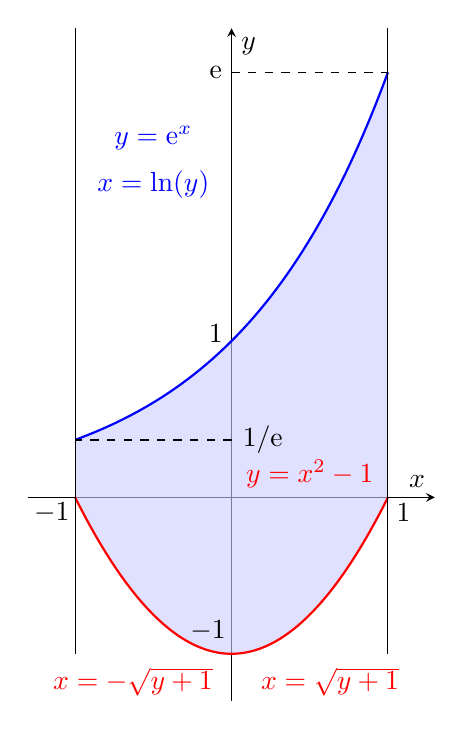
\begin{tikzpicture}
  \begin{axis}[
      axis lines=center,
      axis equal image,
      xlabel={$x$},
      ylabel={$y$},
      xtick=\empty, ytick=\empty,
      xmin=-1.3, xmax=1.3,
      ymin=-1.3, ymax=3,
      samples=200,
      scale=1.5,
      domain=-1:1,
    ]

    \addplot [thick, blue, name path=A, domain=-1:1] {e^x};
    \addplot [thick, red, name path=B] {x^2-1};
    \addplot [blue!20, fill opacity=0.6] fill between[of=A and B,soft clip={domain=-1:1}];
    \draw (-1,-1)--(-1,3); \draw (1,-1)--(1,3); \draw[dashed] (0,2.718)--(1,2.718); \draw[dashed] (0,0.367)--(-1,0.367);


    \node at (axis cs:-1.15,-0.1) {$-1$};
    \node at (axis cs:1.1,-0.1) {$1$};
    \node at (axis cs:-0.1,1.05) {$1$};
    \node at (axis cs:-0.15,-0.85) {$-1$};
    \node at (-0.1,2.718) {$\mathrm{e}$};
    \node at (0.2,0.367) {$1/\mathrm{e}$};
    \node[red] at (0.5,0.15) {$y=x^2-1$};
    \node[red] at (0.63,-1.18) {$x=\sqrt{y+1}$};
    \node[red] at (-0.63,-1.18) {$x=-\sqrt{y+1}$};

    \node[blue] at (-0.5,2.3) {$y=\mathrm{e}^x$};
    \node[blue] at (-0.5,2) {$x=\ln(y)$};

\end{axis}
\end{tikzpicture}
\end{minipage}
\begin{minipage}{0.62\textwidth}
\[\boxed{
\begin{array}{cl}
A=&\displaystyle\int_{-1}^0\left[\left(\sqrt{y+1}\right)-\left(-\sqrt{y+1}\right)\right]\,dy\\\\&+\displaystyle\int_0^{1/\mathrm{e}}\left[(1)-(-1)\right]\,dy+\displaystyle\int_{1/\mathrm{e}}^{\mathrm{e}}\left[(1)-\left(\ln y\right)\right]\,dy
\end{array}}\]
\end{minipage}
\end{center}

\hfill

\noindent 2. The function $f$ is defined where the denominator is not equal to zero. However, the denominator is always positive. Therefore, the domain of $f$ is $\mathbb{R}$.

\hfill

\noindent Let us find the limit at infinity and negative infinity.

\[\lim_{x\to\infty}\frac{4x}{x^2+1}=\lim_{x\to\infty}\frac{4}{x+\frac1x}=0\]

\hfill

\noindent Similarly, at negative infinity, the limit is zero. Therefore, the $x$-axis is a horizontal asymptote. There is no vertical asymptote.

\hfill

\noindent Take the first derivative and find the critical points. Apply the quotient rule.

\[y'=\frac d{dx}\left(\frac{4x}{x^2+1}\right)=\frac{4\cdot\left(x^2+1\right)-4x\cdot(2x)}{\left(x^2+1\right)^2}=\frac{-4x^2+4}{\left(x^2+1\right)^2}\]

\hfill

\noindent The critical points occur at $x=\pm1$. At these points, the first derivative is $0$.

\hfill

\noindent Take the second derivative. Apply the quotient rule again.

\[y''=\frac d{dx}\left(\frac{-4x^2+4}{\left(x^2+1\right)^2}\right)=\frac{\left(-8x\right)\cdot\left(x^2+1\right)^2-\left(-4x^2+4\right)\cdot2\left(x^2+1\right)\cdot(2x)}{\left(x^2+1\right)^4}=\frac{8x\left(x^2-3\right)}{\left(x^2+1\right)^3}\]

\hfill

\noindent The inflection points occur at $x=0$ and $x=\pm\sqrt3$. At these points, the direction of the curvature changes.

\hfill

\noindent Consider some values of the function. Eventually, set up a table and see what the graph looks like in certain intervals.

\[f\left(-\sqrt3\right)=-\sqrt3,\quad f(-1)=-2,\quad f(0)=0,\quad f(1)=2,\quad f\left(\sqrt3\right)=\sqrt3\]

\begin{center}
    \large
    \begin{tabular}{|c|cccccc|} 
    \hline
        $x$&$\left(-\infty,-\sqrt3\right)$&$\left(-\sqrt3,-1\right)$&$\left(-1,0\right)$&$\left(0,1\right)$&$\left(1,\sqrt3\right)$&$\left(\sqrt3,\infty\right)$\\
        \hline
        $y$&$\left(-\sqrt3,0\right)$&$\left(-2, -4\sqrt3\right)$&$(-2,0)$&$(0,2)$&$\left(\sqrt3,2\right)$&$\left(0,\sqrt3\right)$\\
        \hline
        $y'$ sign&-&-&+&+&-&-\\
        \hline
        $y''$ sign&-&+&+&-&-&+\\
        \hline
    \end{tabular}
\end{center}

\hfill

\begin{center}
\begin{tikzpicture}
  \begin{axis}[
    axis lines = center,
    xlabel = $x$, ylabel = $y$,
    domain=-13:13,
    samples=200,
    ymin=-2.2, ymax=2.2,
    xmin=-11, xmax=11,
    restrict y to domain=-5:5,
    enlargelimits=true,
    axis line style={->},
    xtick={-12,-8,-4,4,8,12}, ytick=\empty,
    scale=1.75,
    ]
    \addplot[blue, thick] {4*x/(x^2+1)};
    \draw[dashed](1.732,0)--(1.732,1.732) ;\draw[dashed](1,0)--(1,2); \draw[dashed](0,2)--(1,2); \draw[dashed](0, 1.732)--(1.732,1.732);
    \draw[dashed](-1.732,0)--(-1.732,-1.732) ;\draw[dashed](-1,0)--(-1,-2); \draw[dashed](0,-2)--(-1,-2); \draw[dashed](0, -1.732)--(-1.732,-1.732);
    
    \draw[dashed,red,thick] (-15,0.02)--(15,0.02);

    \node at (-0.75,0.15) {\small $-1$}; \node at (-2.2,0.15) {\small $-\sqrt3$};
    \node at (0.8,-0.15) {\small $1$}; \node at (1.85,-0.15) {\small $\sqrt3$};
    \node at (-0.5,2) {\small $2$}; \node at (-0.7,1.732) {\small $\sqrt3$};
    \node at (0.7,-2) {\small $-2$}; \node at (0.5,-1.732) {\small $-\sqrt3$};
    

  \end{axis}
\end{tikzpicture}
\end{center}

\noindent 3.

\hfill

\noindent (a) Try to rewrite in the form of $\sin x$ and $\cos x$.

\[\int\frac{\tan x}{\sec^4x}\,dx=\int\frac{\sin x}{\cos x}\cdot\cos^4x\,dx=\int\sin x\cdot\cos^3x\,dx=\int\sin x\cdot\left(1-\sin^2x\right)\cdot \cos x\,dx\]

\hfill

\noindent Let $u=\sin x$, then $du=\cos x\,dx$.

\begin{align*}\int\sin x\cdot\left(1-\sin^2x\right)\cdot\cos x\,dx&=\int u\left(1-u^2\right)\,du=\int\left(u-u^3\right)\,du=\frac{u^2}2-\frac{u^4}4+c\\\\&=\boxed{\frac{\sin^2x}2-\frac{\sin^4x}{4}+c,\quad c\in\mathbb{R}}\end{align*}

\newpage

\noindent (b) Use the method of integration by parts.

\[\left.\begin{array}{c}
u=\ln x\implies du=\dfrac1x\,dx\\[1em]
dv=\dfrac1{x^3}\,dx\implies v=-\dfrac1{2x^2}
\end{array}\right\}\rightarrow \int u\,dv=uv-\int v\,du\]

\[\int\frac{\ln x}{x^3}\,dx=-\frac{\ln x}{2x^2}-\int-\frac1{2x^3}\,dx=\boxed{-\frac{\ln x}{2x^2}-\frac1{4x^2}+c,\quad c\in\mathbb{R}}\]

\hfill

\noindent (c) Expand the expression by multiplying and dividing by the conjugate of the denominator.

\begin{align*}\int\frac1{1+\sin x}\,dx&=\int\frac{1-\sin x}{(1+\sin x)(1-\sin x)}\,dx=\int\frac{1-\sin x}{1-\sin^2x}\,dx=\int\frac{1-\sin x}{\cos^2x}\,dx\\\\&=\int\left(\sec^2x-\tan x\sec x\right)\,dx=\boxed{\tan x-\sec x+c,\quad c\in\mathbb{R}}\end{align*}

\hfill

\noindent (d) Use the method of partial fraction decomposition.

\[\int\frac{x+7}{x^2\,(x+2)}\,dx=\int\left(\frac{A}{x}+\frac{B}{x^2}+\frac{C}{x+2}\right)\,dx\]

\[\begin{array}{rc}
A(x)(x+2)+B(x+2)+C\left(x^2\right)&=x+7\\
x^2(A+C)+x(2A+B)+2B&=x+7
\end{array}\]

\hfill

\noindent Equate the coefficients of like terms.

\[\left.\begin{array}{c}
A+C=0\\
2A+B=1\\
2B=7
\end{array}\right\}\implies A=-\dfrac54, \quad B=\dfrac72,\quad C=\dfrac54\]

\hfill

\noindent Rewrite the integral by substituting the values into the unknowns.
\[\int\left(-\frac5{4x}+\frac{7}{2x^2}+\frac5{4(x+2)}\right)\,dx=\boxed{-\frac{5}4\ln\left|x\right|-\frac7{2x}+\frac54\ln\left|x+2\right|+c,\quad c\in\mathbb{R}}\]

\hfill

\noindent 4.
\begin{center}
\begin{minipage}{0.55\textwidth}
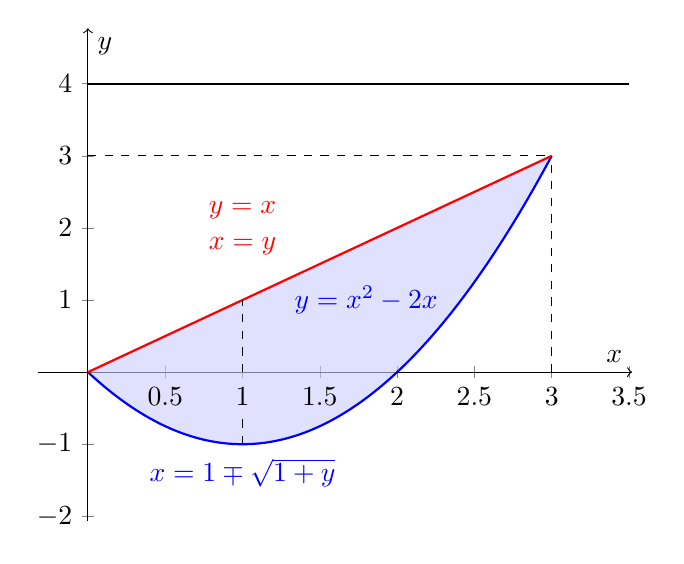
\begin{tikzpicture}
  \begin{axis}[
    axis lines = center,
    xlabel = $x$, ylabel = $y$,
    domain=0:3,
    samples=200,
    ymin=-1.5, ymax=4.2,
    xmin=0, xmax=3.2,
    enlargelimits=true,
    axis line style={->},
    scale=1.1,
    clip=true,
    ]
    \addplot[blue, thick, name path=A] {x^2-2*x};
    \addplot[red, thick, name path=B] {x};
    \addplot[blue!20, draw=none, opacity=0.6] fill between[of=A and B, soft clip={domain=0:3}];

    \draw[thick] (0,4)--(3.5,4);
    \draw[dashed] (1,-1)--(1,-0.6); \draw[dashed] (1,0)--(1,1);
    \draw[dashed] (3,0)--(3,3); \draw[dashed] (0,3)--(3,3);

    \node[red] at (1,2.25) {$y=x$};
    \node[red] at (1,1.75) {$x=y$};

    \node[blue] at (1.8,1) {$y=x^2-2x$};
    \node[blue] at (1,-1.4) {$x=1\mp\sqrt{1+y}$};

  \end{axis}
\end{tikzpicture}
\end{minipage}
\begin{minipage}{0.4\textwidth}
\[V=\int_D2\pi\cdot h(y)\cdot r(y)\,dy\]
\end{minipage}
\end{center}
\begin{align}V&=\int_{-1}^02\pi\left(4-y\right)\left[\left(1+\sqrt{1+y}\right)-\left(1-\sqrt{1+y}\right)\right]\,dy\nonumber\\\nonumber\\&\quad\:+\int_0^{3}2\pi(4-y)\left[\left(1+\sqrt{1+y}\right)-\left(y\right)\right]\,dy\nonumber\\\nonumber\\&=2\pi\int_{-1}^0(4-y)\left(2\sqrt{1+y}\right)\,dy+2\pi\int_0^3(4-y)\left(1+\sqrt{1+y}-y\right)\,dy\end{align}

\hfill

\noindent Evaluate the first integral in $(1)$. Let $u=1+y$, then $du=dy$.

\[y=-1\implies u=0,\qquad y=0\implies u=1\]
\begin{align*}\mathrm{I}_1&=\int_{-1}^0(4-y)\left(2\sqrt{1+y}\right)\,dy=2\int_0^1(5-u)\sqrt u\,du=10\int_0^1\sqrt u\,du-2\int_0^1u^{3/2}\,du\\\\&=\frac{20}3u^{3/2}-\frac45u^{5/2}\Bigg|_0^1=\frac{20}3-\frac45-0=\frac{88}{15}\end{align*}

\hfill

\noindent Evaluate the second integral in $(1)$. Let $u=1+y$, then $du=dy$.

\[y=0\implies u=1,\qquad y=3\implies u=4\]
\begin{align*}\mathrm{I}_2&=\int_0^3(4-y)\left(1+\sqrt{1+y}-y\right)\,dy=\int_1^4(5-u)\left(-u+2+\sqrt u\right)\,du\\\\&=\int_1^4\left(-7u+10+u^2+5\sqrt u-u^{3/2}\right)\,du=\left[-\frac{7u^2}2+10u+\frac{u^3}3+\frac{10}3u^{3/2}-\frac25u^{5/2}\right]_1^4\\\\&=\left[\left(-56+40+\frac{64}3+\frac{80}3-\frac{64}5\right)-\left(-\frac72+10+\frac13+\frac{10}3-\frac25\right)\right]=\frac{283}{30}\end{align*}

\hfill

\noindent Therefore, the result is

\[2\pi\left(\frac{88}{15}+\frac{283}{30}\right)=\boxed{\frac{153\pi}5}\]

\hfill

\noindent 5. If the function $y=f(x)\geq0$ is continuously differentiable on $[a,b]$, the area of the surface generated by revolving the graph of $y=f(x)$ about the $x$-axis is

\[S=\int_a^b2\pi y\sqrt{1+\left(\frac{dy}{dx}\right)^2}\,dx\]

\hfill

\noindent $\dfrac{dy}{dx}=\mathrm{e}^x$. Set $a=0,\:b=1,\:$ and then evaluate the integral.

\[S=\int_0^12\pi\mathrm{e}^x\sqrt{1+\left(\mathrm{e}^x\right)^2}\,dx\]

\hfill

\noindent Let $u=\mathrm{e}^x$, then $du=\mathrm{e}^x\,dx$.

\[x=0\implies u=\mathrm{e}^0=1,\qquad x=1\implies u=\mathrm{e}^1=\mathrm{e}\]

\[S=\int_0^12\pi\mathrm{e}^x\sqrt{1+\left(\mathrm{e}^x\right)^2}\,dx=2\pi\int_1^{\mathrm{e}}\sqrt{1+u^2}\,du\]

\hfill

\noindent We will now use a trigonometric substitution. Let $u=\tan t$ for $\displaystyle0<t<\frac\pi2$, then $du=\sec^2 t\,dt$.

\begin{align*}S&=2\pi\int_1^{\mathrm{e}}\sqrt{1+u^2}\,du=2\pi\int\sqrt{1+\tan^2t}\cdot\sec^2t\,dt=2\pi\int\sqrt{\sec^2t}\cdot\sec^2t\,dt\\\\&=2\pi\int\left|\sec t\right|\sec^2t\,dt=2\pi\int\sec^3t\,dt\qquad\left[\sec t>0\right]\end{align*}

\hfill

\noindent Find the antiderivative of $\sec^3t$ with the help of integration by parts.

\begin{align*}
    w=\sec t\,&\rightarrow\, dw = \sec t\tan t \,dt\\
    dz=\sec^2t\,dt\,&\rightarrow\, z = \tan t
\end{align*}
\begin{align*}
\int\sec^3t\,du&=\tan t\cdot\sec t-\int\tan^2 t\sec t\,dt=\tan t\cdot\sec t-\int\frac{1-\cos^2t}{\cos^3 t}\,dt\\\\&=\tan t\cdot\sec t-\int\sec^3t\,dt+\int\sec t\,dt 
\end{align*}

\hfill

\noindent Notice that the integral appears on the right side of the equation. Therefore,

\[\int\sec^3t\,dt=\frac12\cdot\tan t\cdot\sec t+\frac12\cdot\int\sec t\,dt\]

\hfill

\noindent The integral of $\sec t$ with respect to $t$ is

\[\int\sec t\,dt=\ln\left|\tan t+\sec t\right|+c_1,\quad c_1\in\mathbb{R}\]

\hfill

\noindent Recall $u=\tan t$.

\[u=\tan t\implies u^2=\tan^2t=\sec^2t-1\implies \sec t=\sqrt{u^2+1}\]

\begin{align*}S&=2\pi\cdot\frac12\left(\tan t\cdot\sec t+\ln\left|\tan t+\sec t\right|\right)+c=\pi\left[u\cdot\sqrt{u^2+1}+\ln\left|t+\sqrt{u^2+1}\right|\right]_1^{\mathrm{e}}\end{align*}

\begin{align*}S&=\pi\left[\left(\mathrm{e}\cdot\sqrt{\mathrm{e}^2+1}+\ln\left|\mathrm{e}+\sqrt{\mathrm{e}^2+1}\right|\right)-\left(\sqrt2+\ln\left|1+\sqrt2\right|\right)\right]\\\\&=\boxed{\pi\left[\mathrm{e}\cdot\sqrt{\mathrm{e}^2+1}-\sqrt2+\ln\left(\frac{\mathrm{e}+\sqrt{\mathrm{e}^2+1}}{1+\sqrt2}\right)\right]}\end{align*}

\hfill

\noindent 6. Let the corresponding function be $f(x)=x\mathrm{e}^{-x}$. $f$ is continuous for $x\geq0$. $f$ is positive for $x\geq0$ because $x\geq 0$ and $\mathrm{e}^{-x}$ is positive everywhere. The function is also decreasing for $x\geq1$. Verify this behavior by taking the first derivative of $f$. Apply the product rule.

\[f'(x)=1\cdot\mathrm{e}^{-x}-x\mathrm{e}^{-x}=(1-x)\mathrm{e}^{-x}\]

\hfill

\noindent $f'(x)>0$ for $x\geq1$. The Integral Test states that all the conditions must be satisfied for and after a specific value, for instance $x=1$. Therefore, set the lower bound $x=1$ and evaluate the integral. We will exclusively evaluate the first term of the sequence thereafter.

\[\int_1^{\infty}x\mathrm{e}^{-x}\,dx\]

\hfill

\noindent Apply integration by parts and then evaluate the improper integrals by taking the limit.

\[\left.\begin{array}{c}
u=x\implies du=dv\\[1em]
dv=\mathrm{e}^{-x}\,dx\implies v=-\mathrm{e}^{-x}
\end{array}\right\}\rightarrow \int u\,dv=uv-\int v\,du\]

\begin{align*}\int_1^{\infty}x\mathrm{e}^{-x}\,dx&=\lim_{R\to\infty}\left[-x\mathrm{e}^{-x}\right]_1^R-\lim_{P\to\infty}\int_1^P-\mathrm{e}^{-x}\,dx=\lim_{R\to\infty}\left[-x\mathrm{e}^{-x}\right]_1^R-\lim_{P\to\infty}\mathrm{e}^{-x}\bigg|_1^P\\\\&=\lim_{R\to\infty}\left(-R\mathrm{e}^{-R}+\mathrm{e}^{-1}\right)-\lim_{P\to\infty}\left(\mathrm{e}^{-P}-\mathrm{e}^{-1}\right)=\lim_{R\to\infty}\left(-R\mathrm{e}^{-R}\right)+2\mathrm{e}^{-1}\end{align*}

\hfill

\noindent To evaluate the limit, we assume that $-R\mathrm{e}^{-R}$ is a function of $R$. After that, put the expression in a form that we can apply L'Hôpital's rule in order to eliminate the form $\infty/\infty$.

\[\lim_{R\to\infty}\left(-R\mathrm{e}^{-R}\right)=\lim_{R\to\infty}\frac{-R}{\frac1{\mathrm{e}^{-R}}}\overset{\text{L'H.}}{=}\lim_{R\to\infty}\frac1{\frac{1}{\mathrm{e}^{-2R}}\cdot\left(-\mathrm{e}^{-R}\right)}=\lim_{R\to\infty}\left(-\mathrm{e}^{-R}\right)=0\]

\hfill

\noindent Since the integral converges to $2\mathrm{e}^{-1}$, the series $\displaystyle\sum_{k=1}^{\infty}k\mathrm{e}^{-k}$ also converges. The first term of the series in the original question is $0\cdot\mathrm{e}^0=0$. The sum of a convergent series and a finite number is still finite. Therefore, the sum $\displaystyle\sum_{k=0}^{\infty}k\mathrm{e}^{-k}$ converges.

\newpage

\noindent 7. The Maclaurin series of $f$ is as follows.

\[\sum_{k=0}^{\infty}\frac{f^{(k)}(0)}{k!}x^k\]

\hfill

\noindent Find $f(0),\:f'(0),\:f''(0),\:f'''(0),f^{(4)}(0)$ to look for the pattern.

\[f'(x)=\frac1{1+x},\quad f''(x)=-\frac1{(1+x)^2},\quad f'''(x)=\frac2{(1+x)^3}\quad f^{(4)}(x)=-\frac6{(1+x)^4} \]

\[f(0)=0,\quad f'(0)=1,\quad f''(0)=-1,\quad f'''(0)=2,\quad f^{(4)}(0)=-6\]

\hfill

\noindent This is an alternating sequence where the coefficient of each term is the factorial of the subsequent number starting from $0$ except for $k=0$, that is, the first term of the series. At $k=0$, the first term is $0$. So,

\[f^{k}(0)=\left\{\begin{array}{ll}(-1)^{k-1}\cdot (k-1)!,&\text{if}\: k>0\\0,& \text{if}\:k=0\end{array}\right.\]
\begin{align*}\sum_{k=0}^{\infty}\frac{f^{(k)}(0)}{k!}x^k&=0+\sum_{k=1}^{\infty}\frac{f^{(k)}(0)}{k!}x^k=\sum_{k=1}^{\infty}\frac{(-1)^{k-1}\cdot(k-1)!}{k\cdot(k-1)!}x^k\\\\&=\boxed{\sum_{k=1}^{\infty}\frac{(-1)^{k-1}\cdot x^k}{k}=x-\frac{x^2}2+\frac{x^3}3-\frac{x^4}4+...}\end{align*}

\hfill

\noindent 8. Apply the Ratio Test for absolute convergence, and apply other tests at the endpoints.

\[\lim_{n\to\infty}\left|\frac{(x-2)^{n+1}}{(n+1)\cdot(5)^{n+1}}\cdot\frac{n\cdot5^n}{(x-2)^n}\right|=\lim_{n\to\infty}\left|\frac{\left(x-2\right)\cdot n}{(n+1)\cdot5}\right|=\frac{|x-2|}5\cdot\lim_{n\to\infty}\left|\frac{n}{n+1}\right|=\frac{|x-2|}5\]
\[\frac{|x-2|}5<1\implies |x-2|<5\implies -5<x-2<5\implies -3<x<7 \quad (\text{convergent})\]

\hfill

\noindent Now, take a look at the endpoints.

\[x=-3\implies \sum_{n=1}^{\infty}\frac{(-5)^n}{n\cdot5^n}=\sum_{n=1}^{\infty}\frac{(-1)^n}n\]

\hfill

\noindent This is an alternating series. The non-alternating part, which is $\frac1n$, is nonincreasing for $n\geq1$ and it is positive. The limit at infinity is $0$. By Leibniz's Alternating Series Test, the series converges. Try $x=7$.

\[x=7\implies\sum_{n=1}^{\infty}\frac{(5)^n}{n\cdot5^n}=\sum_{n=1}^{\infty}\frac1n\]

\hfill

\noindent This is a $p$-series with $p=1$, for which the series diverges by the $p$-series Test.

\hfill

\noindent The convergence set for the power series is $\boxed{[-3,7)}$.

\newpage

\begin{center}
2020-2021 Fall Final (18/01/2021) Solutions\\
(Last update: 16/08/2025 15:00)
\end{center}

\noindent 1.
\begin{center}
\begin{minipage}{0.45\linewidth}
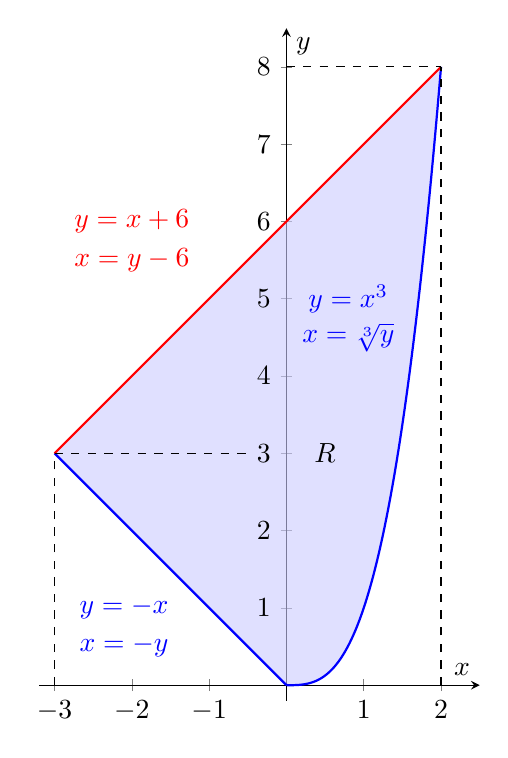
\begin{tikzpicture}
  \begin{axis}[
      axis lines=center,
      axis equal image,
      xlabel={$x$},
      ylabel={$y$},
      xmin=-3.2, xmax=2.5,
      ymin=-0.2, ymax=8.5,
      samples=200,
      scale=1.5,
      domain=-3:2,
    ]

    \addplot [thick, blue, name path=A, domain=-3:2] {max(-x,x^3)};
    \addplot [thick, red, name path=B, domain=-3:2] {x+6};
    \addplot [blue!20, fill opacity=0.6] fill between[of=A and B,soft clip={domain=-3:2}];
    
    \draw[dashed] (-3,0) -- (-3,3); \draw[dashed] (-3,3) -- (-0.5,3);
    \draw[dashed] (2,0) -- (2,8); \draw[dashed] (0,8) -- (2,8);

    \node[red] at (-2,6) {$y=x+6$}; \node[red] at (-2,5.5) {$x=y-6$};
    \node[blue] at (0.8,5) {$y=x^3$}; \node[blue] at (0.8,4.5) {$x=\sqrt[3]{y}$};
    \node[blue] at (-2.1,1) {$y=-x$}; \node[blue] at (-2.1,0.5) {$x=-y$};
    \node at (0.5,3) {$R$};
\end{axis}
\end{tikzpicture}
\end{minipage}\begin{minipage}{0.5\linewidth}
\[\begin{array}{rc}
\text{(i)}&\boxed{\begin{array}{l}\displaystyle\int_{-3}^0\left[(x+6)-(-x)\right]\,dx\\\\\displaystyle+\int_0^2\left[(x+6)-\left(x^3\right)\right]\,dx\end{array}}\\\\\\
\text{(ii)}&\boxed{\begin{array}{l}\displaystyle\int_0^3\left[\left(\sqrt[3]{y}\right)-\left(-y\right)\right]\,dy\\\\\displaystyle+\int_3^8\left[\left(\sqrt[3]{y}\right)-\left(y-6\right)\right]\,dy\end{array}}
\end{array}\]
\end{minipage}
\end{center}

\hfill

\noindent 2.
\begin{center}
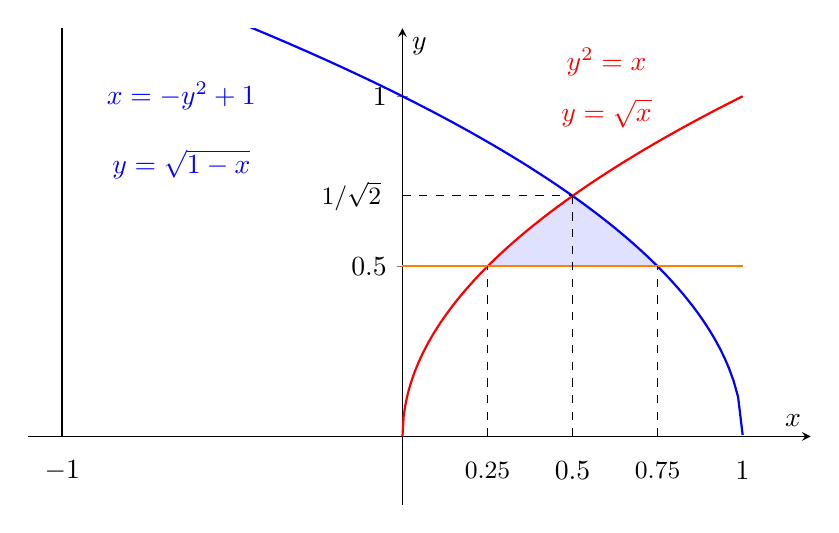
\begin{tikzpicture}
  \begin{axis}[
      axis lines=center,
      axis equal image,
      xlabel={$x$},
      ylabel={$y$},
      xmin=-1.1, xmax=1.2,
      ymin=-0.2, ymax=1.2,
      clip=true,
      scale=1.45,
      xtick=\empty,
    ]

    \addplot [thick, blue, name path=A,samples=150, domain=-1:1] {sqrt(1-x)};
    \addplot [thick, red, name path=B,samples=300, domain=0:1] {sqrt(x)};
    \addplot [thick, orange, name path=C, domain=0:1] {1/2};
    \addplot [blue!20, fill opacity=0.6] fill between[of=B and C,soft clip={domain=0.25:0.5}];
    \addplot [blue!20, fill opacity=0.6] fill between[of=A and C,soft clip={domain=0.5:0.75}];

    \draw[thick] (-1,0)--(-1,2); \draw[dashed] (0.25,0)--(0.25,0.5); \draw[dashed] (0.75,0)--(0.75,0.5); \draw[dashed] (0.5,0)--(0.5,0.707); \draw[dashed] (0,0.707)--(0.5,0.707);
    \node at (0.25,-0.1) {\small$0.25$}; \node at (0.75,-0.1) {\small$0.75$}; \node at (-0.15,0.707) {\small$1/\sqrt2$};

    \node[blue] at (-0.65,1) {$x=-y^2+1$}; \node[blue] at (-0.65,0.8) {$y=\sqrt{1-x}$};
    \node[red] at (0.6,1.1) {$y^2=x$}; \node[red] at (0.6,0.95) {$y=\sqrt{x}$};

    \node at (-1,-0.1) {$-1$}; \node at (1,-0.1) {$1$}; \node at (0.5,-0.1) {$0.5$};
    
  \end{axis}
\end{tikzpicture}
\end{center}

\noindent (i)
\[\boxed{\int_{1/4}^{1/2}2\pi(x+1)\left[\left(\sqrt x\right)-\left(\frac12\right)\right]\,dx+\int_{1/2}^{3/4}2\pi(x+1)\left[\left(\sqrt{1-x}\right)-\left(\frac12\right)\right]\,dx}\]

\hfill

\noindent (ii)
\[\boxed{\int_{1/2}^{1/\sqrt{2}}\pi\left[\left(-y^2+1+1\right)^2-\left(y^2+1\right)^2\right]\,dy}\]

\newpage

\noindent 3.

\hfill

\noindent (a) Let $u=\sqrt[3]{x}+4$, then $du=\dfrac1{3x^{2/3}}\,dx$.

\[\int\frac{dx}{x^{2/3}\left(\sqrt[3]{x}+4\right)}=\int\frac{3du}{u}=3\ln\left|u\right|+c=\boxed{3\ln\left|\sqrt[3]{x}+4\right|+c,\quad c\in\mathbb{R}}\]

\hfill

\noindent (b) Apply integration by parts.

\[\left.\begin{array}{c}
u=(\ln x)^2\implies du=2\ln x\cdot\dfrac1x\,dx\\
dv=dx\implies v=x
\end{array}\right\}\rightarrow \int u\,dv=uv-\int v\,du\]

\[\int(\ln x)^2\,dx=x(\ln x)^2-\int2\ln x\,dx\]

\hfill

\noindent Apply integration by parts once again.

\[\left.\begin{array}{c}
u=\ln x\implies du=\dfrac1x\,dx\\
dv=dx\implies v=x
\end{array}\right\}\rightarrow \int u\,dv=uv-\int v\,du\]

\[\int(\ln x)^2\,dx=x(\ln x)^2-\int2\ln x\,dx\]

\[x(\ln x)^2-\int2\ln x\,dx=x(\ln x)^2-2\left[x\ln x-\int dx\right]=\boxed{x(\ln x)^2-2x\ln x+2x+c,\: c\in\mathbb{R}}\]

\hfill

\noindent (c) Let $x=\sqrt3\tan u$ for $0<u<\dfrac\pi2$, then $dx=\sqrt3\sec^2u\,du$.

\begin{align*}\int\frac{dx}{\sqrt{3+x^2}}&=\int\frac{\sqrt3\sec^2u}{\sqrt{3+3\tan^2u}}\,du=\int\frac{\sec^2u}{\sqrt{1+\tan^2u}}\,du=\int\frac{\sec^2u}{\left|\sec u\right|}\,du\\\\&=\int\sec u\,du\qquad\left[\sec u>0\right]\\\\&=\ln\left|\tan u+\sec u\right|+c,\quad c\in\mathbb{R}\end{align*}

\hfill

\noindent Recall $x=\sqrt3\tan u$.

\[x^2=3\tan^2u=3\sec^2u-3\implies \sec^2u=\frac{x^2+3}3\implies\sec u=\frac{\sqrt{x^2+3}}{\sqrt3}\]

\[\ln\left|\tan u+\sec u\right|+c=\boxed{\ln\left|\frac{x}{\sqrt3}+\frac{\sqrt{x^2+3}}{\sqrt3}\right|+c,\quad c\in\mathbb{R}}\]

\noindent We can omit the constant part.

\[\boxed{\ln\left(x+\sqrt{x^2+3}\right)+c,\quad c\in\mathbb{R}}\]

\hfill

\noindent (d) We may utilize the tangent half-angle substitution, which is also called the Weierstrass substitution. Let $\displaystyle t=\tan\left(\frac x2\right)$. After some mathematical operations, we get the following.

\[\sin x={\frac{2t}{1+t^{2}}},\quad\cos x={\frac{1-t^{2}}{1+t^{2}}},\quad dx={\frac2{1+t^{2}}}\,dt\]

\begin{align*}\int\frac{dx}{2+\sin x}&=\int\frac2{1+t^2}\cdot\frac1{2+\frac{2t}{1+t^2}}\,dt=\int\frac{dt}{t^2+t+1}=\int\frac{dt}{t^2+t+\frac14+\frac34}\\\\&=\int\frac{dt}{\left(t+\frac12\right)^2+\frac34}=\frac43\int\frac{dt}{\frac43\left(t+\frac12\right)^2+1}=\frac43\int\frac{dt}{\left(\frac2{\sqrt3}\right)^2\left(t+\frac12\right)^2+1}\end{align*}

\hfill

\noindent Let $\displaystyle u=\frac2{\sqrt3}\left(t+\frac12\right)$, then $\displaystyle du=\frac2{\sqrt3}\,dt$.

\begin{align*}\frac{2\sqrt3}3\int\frac{du}{u^2+1}&=\frac{2\sqrt3}3\arctan u+c=\frac{2\sqrt3}3\arctan\left(\frac2{\sqrt3}\left(t+\frac12\right)\right)+c\\\\&=\boxed{\frac{2\sqrt3}3\arctan\left(\frac2{\sqrt3}\left(\tan\left(\frac x2\right)+\frac12\right)\right)+c,\quad c\in\mathbb{R}}\end{align*}

\hfill

\noindent 4. Take $f(x)=\dfrac{x^2+1}{x^3}$. We have $f'(x)=-\dfrac{x^2+3}{x^4}<0$ for all $x\geq1$. That means $f$ is decreasing for $x\geq1$. We also have

\[f(1)=2,\quad \lim_{x\to\infty}f(x)=\lim_{x\to\infty}\left(\frac1x +\frac1{x^3}\right)\qquad \implies0<f(x)\leq2,\quad x\geq1\]

\hfill

\noindent Since the sequence is bounded and monotonic, by the Monotone Convergence Theorem, the sequence converges.

\hfill

\noindent 5. Take the corresponding function $\displaystyle f(x)=\frac1{x^4+x^2}$. $f$ is positive for $x\geq1$ because $x^4>0$ and $x^2>0$. $f$ is also continuous for $x\geq1$ because the denominator is a polynomial whose \textit{only} root is zero, which is out of the boundary of the integral. Investigate the monotonicity of $f$ by taking the first derivative.

\[f'(x)=-\frac{4x^3+2x}{\left(x^4+x^2\right)^2}\implies f'(x)\leq0\:\text{for}\:x\geq1\]

\hfill

\noindent We may now apply the Integral Test since the criteria have been satisfied.

\begin{align*}\int_1^{\infty}\frac{dx}{x^4+x^2}&=\int_1^{\infty}\frac{dx}{x^2\left(x^2+1\right)}=\int_1^{\infty}\left(\frac1{x^2}-\frac1{x^2+1}\right)\,dx\\\\&=\lim_{R\to\infty}\int_1^R\left(\frac1{x^2}-\frac1{x^2+1}\right)\,dx=\lim_{R\to\infty}\left[-\frac1x-\arctan x\right]_1^R\\\\&=\lim_{R\to\infty}\left[\left(-\frac1R-\arctan R\right)-\left(-1-\arctan1\right)\right]=1-\frac\pi4\quad\left(\text{convergent}\right)\end{align*}

\hfill

\noindent By the Integral Test, the series $\displaystyle\sum_{k=1}^{\infty}\frac1{k^4+k^2}$ also converges.

\hfill

\noindent 6. Apply the Ratio Test for absolute convergence, and apply other tests at the endpoints.

\[\lim_{n\to\infty}\left|\frac{(x+1)^{k+1}}{2(k+1)}\cdot\frac{2k}{(x+1)^k}\right|=\lim_{n\to\infty}\left|\frac{(x+1)\cdot k}{k+1}\right|=|x+1|\cdot\lim_{n\to\infty}\left|\frac{k}{k+1}\right|=|x+1|\]
\[|x+1|<1\implies-1<x+1<1\implies-2<x<0\quad(\text{convergent})\]

\hfill

\noindent Now, take a look at the endpoints.

\[x=-2\rightarrow\sum_{k=1}^{\infty}\frac{(-1)^k}{2k}=\frac12\sum_{k=1}^{\infty}\frac{(-1)^k}k\]

\hfill

\noindent This is an alternating series. The non-alternating part, which is $\frac1k$, is nonincreasing for $k\geq1$ and it is positive. The limit at infinity is $0$. By Leibniz's Alternating Series Test, the series converges. Try $x=0$.

\[x=0\rightarrow\sum_{k=1}^{\infty}\frac{1^k}{2k}=\frac12\sum_{k=1}^{\infty}\frac1k\]

\hfill

\noindent This is a $p$-series with $p=1$, for which the series diverges by the $p$-series Test.

\hfill

\noindent The convergence set for the power series is

\[\boxed{[-2, 0)}\]

\hfill

\noindent 7. The Maclaurin series of $\sin x$ is

\[\sum_{n=0}^{\infty}\frac{(-1)^nx^{2n+1}}{(2n+1)!}=x-\frac{x^3}{3!}+\frac{x^5}{5!}-\frac{x^7}{7!}+...\]

\hfill

\noindent Rewrite the limit using this expansion.

\[\lim_{x\to0}\frac{\sin x}{x}=\lim_{x\to0}\left[\frac1x\cdot \left(x-\frac{x^3}{3!}+\frac{x^5}{5!}-\frac{x^7}{7!}+...\right)\right]=\lim_{x\to0}\left(1-\frac{x^2}{3!}+\frac{x^4}{5!}-\frac{x^6}{7!}+...\right)=\boxed{1}\]

\newpage

\begin{center}
2021-2022 Final (07/01/2022) Solutions\\
(Last update: 16/08/2025 21:36)
\end{center}

\noindent 1.

\hfill

\noindent (a) Use the method of partial fraction decomposition.

\[\int\frac{dx}{x^3-4x^2+3x}=\int\frac{dx}{x(x-3)(x-1)}=\int\left(\frac Ax+\frac B{x-3}+\frac C{x-1}\right)\,dx\]

\[\begin{array}{rc}A(x-3)(x-1)+Bx(x-1)+Cx(x-3)&=1\\x^2(A+B+C)+x(-4A-B-3C)+3A&=1\\&\end{array}\]

\hfill

\noindent Equate the coefficients of like terms.

\[\left.\begin{array}{r}
x^2(A+B+C)=0\\
x(-4A-B-3C)=0\\
3A=1
\end{array}\right\}\rightarrow A=\frac13,\qquad\left.\begin{array}{r}
B+C=-\dfrac13\\[1em]
B+3C=-\dfrac43
\end{array}\right\}\rightarrow B=\frac16,\quad C=-\frac12\]

\hfill

\noindent Rewrite the integral.

\begin{align*}
\int\left(\frac Ax+\frac B{x-3}+\frac C{x-1}\right)\,dx&=\int\left(\frac1{3x}+\frac1{6(x-3)}-\frac1{2(x-1)}\right)\,dx\\\\&=\boxed{\frac13\ln|x|+\frac16\ln|x-3|-\frac12\ln|x-1|+c,\quad c\in\mathbb{R}}
\end{align*}

\hfill

\noindent (b) The limit is in the indeterminate form $0/0$. Apply L'Hôpital's rule to eliminate the indeterminate form.

\[\lim_{x\to\textstyle\frac\pi2}\frac{\displaystyle\int_{\pi/2}^x\ln(\sin t)\,dt}{\sin x-1}\overset{\text{L'H.}}{=}\lim_{x\to\textstyle\frac\pi2}\frac{\displaystyle\frac d{dx}\int_{\pi/2}^x\ln(\sin t)\,dt}{\cos x}\]

\hfill

\noindent By the Fundamental Theorem of Calculus, we may rewrite the limit as follows.

\begin{align*}\lim_{x\to\textstyle\frac\pi2}\frac{\displaystyle\frac d{dx}\int_{\pi/2}^x\ln(\sin t)\,dt}{\cos x}&=\lim_{x\to\textstyle\frac\pi2}\frac{\ln(\sin x)}{\cos x}\overset{\text{L'H.}}{=}\lim_{x\to\textstyle\frac\pi2}\frac{\frac1{\sin x}\cdot\cos x}{-\sin x}=\lim_{x\to\textstyle\frac\pi2}\frac{\cos x}{-\sin^2x}=-\frac{\cos\frac\pi2}{\sin^2\frac\pi2}\\\\&=\boxed0\end{align*}

\hfill

\noindent (c) Take the limit as this is an improper integral.

\[\int_1^2\frac{dx}{(x-1)^{2/3}}=\lim_{R\to1^+}\int_R^2\frac{dx}{(x-1)^{2/3}}=\lim_{R\to1^+}3(x-1)^{1/3}\bigg|_R^2=3\lim_{R\to1^+}\left(1-(R-1)^{1/3}\right)=\boxed3\]

\newpage

\noindent 2.
\begin{center}
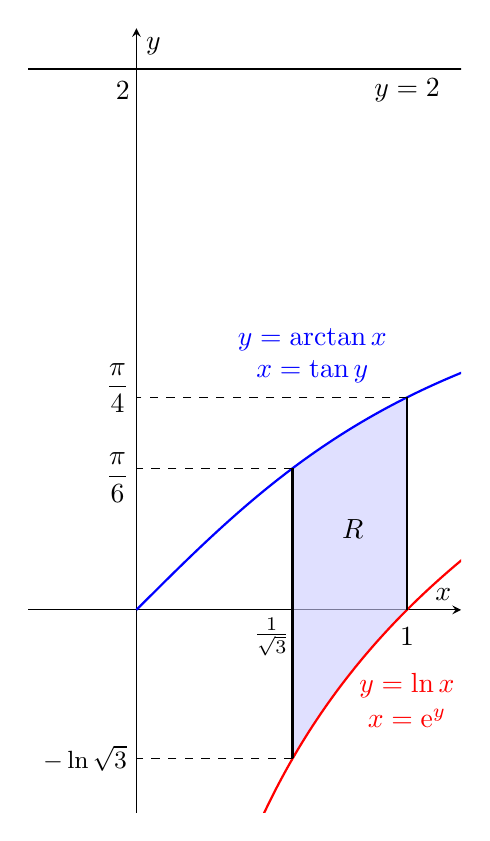
\begin{tikzpicture}
  \begin{axis}[
      axis lines=center,
      axis equal image,
      xlabel={$x$},
      ylabel={$y$},
      xmin=-0.4, xmax=1.2,
      ymin=-0.75, ymax=2.15,
      samples=200,
      scale=1.75,
      domain=0.577:1,
      xtick=\empty, ytick=\empty,
    ]

    \addplot [thick, blue, name path=A, domain=0:2] {rad(atan(x))};
    \addplot [thick, red, name path=B, domain=0.1:2] {ln(x)};
    \addplot [blue!20, fill opacity=0.6] fill between[of=A and B,soft clip={domain=0.577:1}];
    
    \draw[dashed] (-3,0) -- (-3,3); \draw[dashed] (-3,3) -- (-0.5,3);
    \draw[dashed] (2,0) -- (2,8); \draw[dashed] (0,8) -- (2,8);

    \node[blue] at (0.65,1) {$y=\arctan x$}; \node[blue] at (0.65,0.88) {$x=\tan y$};
    \node[red] at (1,-0.28) {$y=\ln x$}; \node[red] at (1,-0.4) {$x=\mathrm{e}^y$};

    \draw[thick] (0.577,-0.549)--(0.577,0.523); \draw[thick] (1,0)--(1,0.785);
    \draw[dashed] (1,0.785)--(0,0.785); \draw[dashed] (0.577, 0.523)--(0,0.523);
    \draw[dashed] (0.577,-0.549)--(0,-0.549);
    \draw[thick] (-1,2)--(2,2); 
    
    \node at (0.8,0.3) {$R$}; \node at (0.5,-0.1) {$\frac1{\sqrt3}$}; \node at (-0.07,0.49) {$\dfrac\pi6$}; \node at (-0.07,0.82) {$\dfrac\pi4$}; \node at (-0.19,-0.549) {\small $-\ln\sqrt3$}; \node at (1,-0.1) {$1$}; \node at (-0.05,1.92) {$2$}; \node at (1,1.92) {$y=2$};
\end{axis}
\end{tikzpicture}
\end{center}
\noindent (a)
\begin{equation}A=\int_{1/\sqrt3}^1\left(\arctan x-\ln x\right)\,dx=\int_{1/\sqrt3}^1\arctan x\,dx-\int_{1/\sqrt3}^1\ln x\,dx\end{equation}

\hfill

\noindent Calculate the first integral in $(1)$ by integration by parts.

\[\left.\begin{array}{c}
u=\arctan x\implies du=\dfrac1{x^2+1}\,dx\\[1em]
dv=dx\implies v=x
\end{array}\right\}\rightarrow \int u\,dv=uv-\int v\,du\]

\begin{align*}\int_{1/\sqrt3}^1\arctan x\,dx&=x\arctan x\bigg|_{1/\sqrt3}^1-\int_{1/\sqrt3}^1\frac{x}{x^2+1}\,dx=\left(x\arctan x-\frac12\ln\left|x^2+1\right|\right)\Bigg|_{1/\sqrt3}^1\\\\&=\left(\frac\pi4-\frac{\ln 2}2\right)-\left(\frac{\pi\sqrt3}{18}-\frac12\cdot\ln\left(\frac43\right)\right)=\frac{\pi\left(9-2\sqrt3\right)}{36}+\frac12\cdot\ln\frac23\end{align*}

\hfill

\noindent Calculate the second integral in $(1)$ by integration by parts.

\[\left.\begin{array}{c}
u=\ln x\implies du=\dfrac1x\,dx\\[1em]
dv=dx\implies v=x
\end{array}\right\}\rightarrow \int u\,dv=uv-\int v\,du\]

\begin{align*}\int_{1/\sqrt3}^1\ln x\,dx&=x\ln x\bigg|_{1/\sqrt3}^1-\int_{1/\sqrt3}^1\,dx=\left(x\ln x-x\right)\Bigg|_{1/\sqrt3}^1=\left(0-1\right)-\left(-\frac{\ln\sqrt3}{\sqrt3}-\frac1{\sqrt3}\right)\\\\&=\frac{\sqrt3\ln\sqrt3+\sqrt3-3}3\end{align*}

\hfill

\noindent The result is then

\[A=\boxed{\frac{\pi\left(9-2\sqrt3\right)}{36}+\frac12\cdot\ln\frac23-\frac{\sqrt3\ln\sqrt3+\sqrt3-3}3}\]

\hfill

\noindent (b)
\begin{align*}\boxed{\begin{array}{l}\displaystyle\int_{-\ln\sqrt3}^0\pi\left[\left(\mathrm{e}^y\right)^2-\left(\frac1{\sqrt3}\right)^2\right]\,dy+\int_0^{\pi/6}\pi\left[(1)^2-\left(\frac1{\sqrt3}\right)^2\right]\,dy\\\\\displaystyle+\int_{\pi/6}^{\pi/4}\pi\left[(1^2)-\left(\tan y\right)^2\right]\,dy\end{array}}\end{align*}

\hfill

\noindent (c)
\begin{align*}\boxed{\begin{array}{l}\displaystyle\int_{-\ln\sqrt3}^02\pi\left(2-y\right)\left(\mathrm{e}^y-\frac1{\sqrt3}\right)\,dy+\int_0^{\pi/6}2\pi\left(2-y\right)\left(1-\frac1{\sqrt3}\right)\,dy\\\\\displaystyle+\int_{\pi/6}^{\pi/4}2\pi\left(2-y\right)\left(1-\tan y\right)\,dy\end{array}}\end{align*}

\hfill

\noindent 3.

\hfill

\noindent (a) Determine the $n$th partial sum.

\begin{align*}\sum_{n=1}^{\infty}\left(\arctan n -\arctan(n-1)\right)&=\left(\cancel{\arctan1}-\arctan0\right)+\left(\cancel{\arctan2}-\cancel{\arctan1}\right)\\&\quad\:+\left(\cancel{\arctan3}-\cancel{\arctan2}\right)+\left(\cancel{\arctan4}-\cancel{\arctan3}\right)+...\\\\&\quad\:+\left(\arctan n-\cancel{\arctan(n-1)}\right)=\arctan n-\arctan0\\\\&=\arctan n\end{align*}

\[\lim_{n\to\infty}\arctan n=\frac\pi2\quad(\text{convergent})\]

\hfill

\noindent Therefore, the series $\displaystyle\sum_{n=1}^{\infty}\left(\arctan n -\arctan(n-1)\right)$ converges.

\hfill

\noindent (b)
\begin{align*}\sum_{n=0}^{\infty}\frac{(-3)^{n+1}}{2^{3n}}=\sum_{n=0}^{\infty}\frac{-3\cdot(-3)^n}{8^n}=-3\sum_{n=0}^{\infty}\left(-\frac38\right)^n\end{align*}

\hfill

\noindent This is a geometric series where $r=-\dfrac38$. $|r|=\dfrac38<1$. Therefore, the series $\displaystyle\sum_{n=0}^{\infty}\frac{(-3)^{n+1}}{2^{3n}}$ converges.

\hfill

\noindent (c) Apply the $n$th Term Test for divergence. We may take the limit inside the trigonometric function because $\cos x$ is continuous everywhere. Since $1+n^4$ grows faster than $n^2$, the value of the expression $\dfrac{n^2}{1+n^4}$ tends to zero.

\[\lim_{n\to\infty}\cos\left(\frac{n^2}{1+n^4}\right)=\cos\left[\lim_{n\to\infty}\left(\frac{n^2}{1+n^4}\right)\right]=\cos0=1\neq0\]

\hfill

\noindent By the $n$th Term Test for divergence, the series $\displaystyle\sum_{n=1}^\infty\cos\left(\frac{n^2}{1+n^4}\right)$ diverges.

\hfill

\noindent (d) Take $\displaystyle f(x)=\frac1{x(\ln x)^2}$. $f$ is positive and decreasing for $x\geq2$ because $x$ and $(\ln x)^2$ are positive and increasing for $x\geq2$. $x$ is a polynomial which is defined everywhere and $(\ln x)^2$ is continuous for $x\geq2$. Since we took into account every criterion, we may apply the Integral Test. Handle the improper integrals by taking the limit.

\[\int_2^{\infty}\frac{dx}{x(\ln x)^2}=\lim_{R\to\infty}\int_2^R\frac{dx}{x(\ln x)^2}=\lim_{R\to\infty}\left[-\frac1{\ln x}\right]_2^R=\lim_{R\to\infty}\left[-\frac1{\ln R}+\frac1{\ln2}\right]=\frac1{\ln 2}\]

\hfill

\noindent Since the integral converges, the series $\displaystyle\sum_{n=2}^\infty\frac1{n(\ln n)^2}$ also converges.

\newpage

\begin{center}
2022-2023 Final (11/01/2023) Solutions\\
(Last update: 18/08/2025 01:51)
\end{center}

\noindent 1.

\hfill

\noindent (a) The volume of a sphere with radius $r$ is

\[V=\frac43\pi r^3\]

\hfill

\noindent The differential of $V$ is

\[dV=4\pi r^2\,dr\]

\hfill

\noindent The maximum error is known to be $1/8$ inches. So, $|dr|\leq1/8$. The maximum propagated error is then

\[dV=4\pi\cdot14^2\cdot\dfrac18=\boxed{98\pi\:\text{in}^3.}\]

\hfill

\noindent (b) $|dV|=2$ at most. Solve the differential form for $dr$.

\[dr=\frac{dV}{4\pi r^2}=\frac{2}{4\pi\cdot 14^2}=\boxed{\frac1{392\pi}\:\text{inches}}\]

\hfill

\noindent 2.

\hfill

\noindent (a) Let $x=u^2$, then $u=\sqrt x$ and $dx=2u\,du$.

\begin{align*}\int\frac{dx}{\sqrt x\,\left(\sqrt x+2\right)}&=\int\frac{2u}{u(u+2)}\,du=2\int\frac{du}{u+2}=2\ln|u+2|+c\\\\&=\boxed{2\ln\left|\sqrt x+2\right|+c,\: c\in\mathbb{R}}\end{align*}

\hfill

\noindent (b) This question is beyond the scope of the curriculum, and students are not expected to solve it using the knowledge they have acquired in this course.

\hfill

\noindent (c) Let $x=\sqrt3\sin u$ for $-\dfrac\pi2<u<\dfrac\pi2$, then $dx=\sqrt3\cos u\,du$.

\begin{align*}\int\frac{dx}{\sqrt{3-x^2}}&=\int\frac{\sqrt3\cos u}{\sqrt{3-3\sin^2u}}\,du=\int\frac{\cos u}{\sqrt{\cos^2u}}\,du=\int\frac{\cos u}{|\cos u|}\,du\\\\&=\int\frac{\cos u}{\cos u}\,du\quad\left[\cos u>0\right]\\\\&=\int du=u+c\end{align*}

\hfill

\noindent If $x=\sqrt3\sin u$, then $\sin u=\dfrac x{\sqrt3}\implies u=\arcsin\left(\dfrac x{\sqrt3}\right)$. The answer is then

\hfill

\[\boxed{\arcsin\left(\frac x{\sqrt3}\right)+c,\quad c\in\mathbb{R}}\]

\hfill

\noindent (d) We may utilize the tangent half-angle substitution, which is sometimes called the Weierstrass substitution. Let $\displaystyle t = \tan\left(\frac x2\right)$. Then

\begin{equation*}
\sin x={\frac{2t}{1+t^{2}}},\quad\cos x={\frac{1-t^{2}}{1+t^{2}}},\quad dx={\frac2{1+t^{2}}}\,dt
\end{equation*}

\hfill

\noindent Rewrite the integral.

\[\int\frac{dx}{2+\cos x}=\int\frac{\dfrac2{1+t^2}}{2+\dfrac{1-t^2}{1+t^2}}\,dt=\int\frac{2}{3+t^2}\,dt=\int\frac{2}{3\left(1+\dfrac{t^2}3\right)}\,dt=\frac23\int\frac1{1+\left(\dfrac t{\sqrt3}\right)^2}\,dt\]

\hfill

\noindent Let $u=\dfrac t{\sqrt3}$, then $\sqrt3\,du=dt$.

\begin{align*}\frac23\int\frac{dt}{1+\left(\dfrac t{\sqrt3}\right)^2}&=\frac{2\sqrt3}3\int\frac{du}{1+u^2}=\frac{2\sqrt3}3\arctan u+c=\frac{2\sqrt3}3\arctan\frac t{\sqrt3}+c\\&=\boxed{\frac{2\sqrt3}3\arctan\left(\frac1{\sqrt3}\tan\left(\frac x2\right)\right)+c,\quad c\in\mathbb{R}}\end{align*}

\hfill

\noindent 3.
\begin{center}
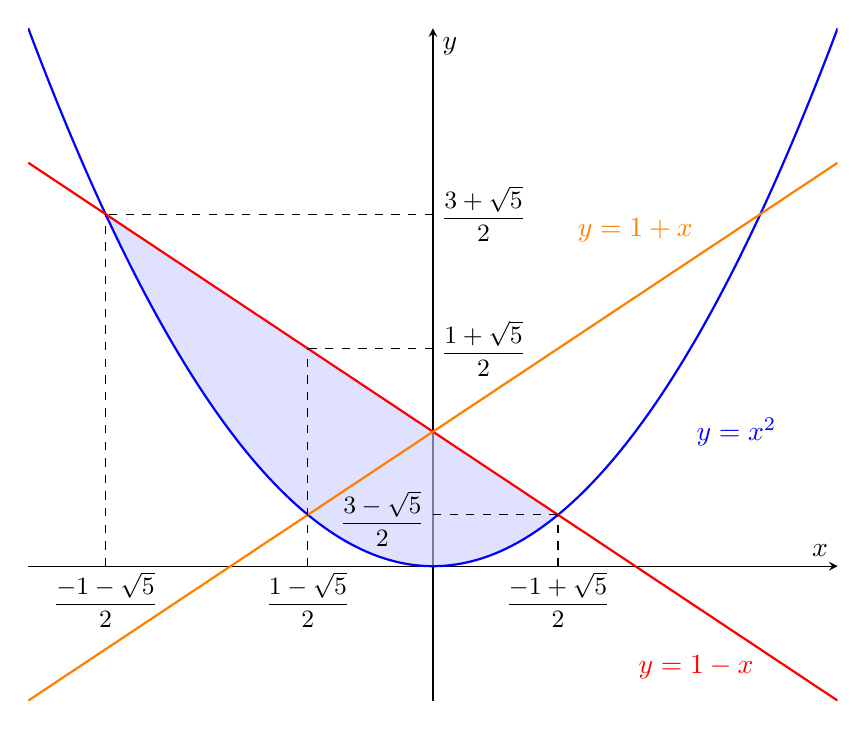
\begin{tikzpicture}
  \begin{axis}[
      axis lines=center,
      xlabel={$x$},
      ylabel={$y$},
      ytick=\empty, xtick=\empty,
      xmin=-2, xmax=2,
      ymin=-1, ymax=4,
      samples=250,
      clip=true,
      scale=1.5,
      domain=-2:2,
    ]

    \addplot [thick, blue, name path=A] {x^2};
    \addplot [thick, red, name path=B] {-x+1};
    \addplot [thick, orange] {x+1};
    \addplot [blue!20, fill opacity=0.6] fill between[of=A and B, soft clip={domain=-1.618:0.618}];
    
    \node at (-1.618,-0.25) {\small $\displaystyle\frac{-1-\sqrt5}2$};
    \node at (0.618,-0.25) {\small $\displaystyle\frac{-1+\sqrt5}2$};
    \node at (0.25,2.618) {\small $\displaystyle\frac{3+\sqrt5}2$};
    \node at (-0.25,0.35) {\small $\displaystyle\frac{3-\sqrt5}2$};
    \node at (0.25,1.618) {\small $\displaystyle\frac{1+\sqrt5}2$};
    \node at (-0.618,-0.25) {\small $\displaystyle\frac{1-\sqrt5}2$};
    
    \node[red] at (1.3,-0.75) {$y=1-x$};
    \node[orange] at (1,2.5) {$y=1+x$};
    \node[blue] at (1.5,1) {$y=x^2$};

    \draw[dashed] (-1.618,0)--(-1.618,2.618); \draw[dashed] (0,2.618)--(-1.618,2.618);
    \draw[dashed] (0.618,0)--(0.618,0.381); \draw[dashed] (0,0.381)--(0.618,0.381);
    \draw[dashed] (-0.618,0)--(-0.618,1.618); \draw[dashed] (0,1.618)--(-0.618,1.618);

  \end{axis}
\end{tikzpicture}
\end{center}

\noindent We have the symmetry of the region that is bounded to the right of the $y$-axis. Therefore, it is not necessary to apply the method to the symmetrical region on the left. The volume of this solid is

\[\boxed{\begin{array}{l}\displaystyle\int_{\textstyle\frac{-1-\sqrt5}2}^{\textstyle\frac{1-\sqrt5}2}2\pi(-x)\left[\left(1-x\right)-\left(x^2\right)\right]\,dx\\\displaystyle+\int_{\textstyle\frac{1-\sqrt5}2}^02\pi(-x)\left[\left(1-x\right)-\left(1+x\right)\right]\,dx+\int_0^{\textstyle\frac{-1+\sqrt5}2}2\pi(x)\left[\left(1-x\right)-\left(x^2\right)\right]\,dx\end{array}}\]

\hfill

\noindent 4. If the function $y=f(x)\geq0$ is continuously differentiable on $[a,b]$, the area of the surface generated by revolving the graph of $y=f(x)$ about the $x$-axis is

\[S=\int_a^b2\pi y\sqrt{1+\left(\frac{dy}{dx}\right)^2}\,dx\]

\hfill

\noindent $\dfrac{dy}{dx}=\dfrac{x^2}2-\dfrac1{2x^2}$. Set $a=1/2,\:b=1\:$ and then evaluate the integral.

\begin{align*}S&=\int_{1/2}^12\pi\left(\frac{x^3}6+\frac1{2x}\right)\sqrt{1+\left(\frac{x^2}2-\frac1{2x^2}\right)^2}\,dx\\\\&=\int_{1/2}^12\pi\left(\frac{x^3}6+\frac1{2x}\right)\sqrt{1+\frac{x^4}4-\frac12+\frac1{4x^4}}\,dx=\int_{1/2}^12\pi\left(\frac{x^3}6+\frac1{2x}\right)\sqrt{\frac{x^4}4+\frac12+\frac1{4x^4}}\,dx\\\\&=\int_{1/2}^12\pi\left(\frac{x^3}6+\frac1{2x}\right)\sqrt{\left(\frac{x^2}2+\frac1{2x^2}\right)^2}\,dx=\int_{1/2}^12\pi\left(\frac{x^3}6+\frac1{2x}\right)\left(\frac{x^2}2+\frac1{2x^2}\right)\,dx\\\\&=\int_{1/2}^12\pi\left(\frac{x^5}{12}+\frac x{12}+\frac x4+\frac1{4x^3}\right)\,dx=2\pi\left[\frac{x^6}{72}+\frac{x^2}{24}+\frac{x^2}8-\frac1{8x^2}\right]_{1/2}^1\\\\&=2\pi\left[\left(\frac1{72}+\frac1{24}+\frac{1}8-\frac18\right)-\left(\frac1{4608}+\frac1{96}+\frac1{32}-\frac12\right)\right]=\boxed{\frac{2367\pi}{2304}}\end{align*}

\hfill

\noindent 5. Take the corresponding function $f(x)=\dfrac2{3x+5}$. The function is continuous for $x\geq1$ because the denominator is a first-degree polynomial whose root is $x_0=-\dfrac53<1$. $f$ is also positive and increasing for $x\geq1$. Since the criteria hold, we may apply the Integral Test. Handle the improper integral by taking the limit.

\begin{align*}\int_1^{\infty}\frac{2}{3x+5}\,dx&=\lim_{R\to\infty}\int_1^R\frac{2}{3x+5}\,dx=\lim_{R\to\infty}\frac23\ln|3x+5|\bigg|_1^R=\frac23\lim_{R\to\infty}\left(\ln|3R+5|-\ln8\right)\\\\&=\infty\end{align*}

\noindent Since the integral diverges, by the Integral Test, the series $\displaystyle\sum_{n=1}^{\infty}\frac2{3n+5}$ also diverges.

\hfill

\noindent 6. Recall the equality $\dfrac1{x(x+1)}=\dfrac1{x}-\dfrac1{x+1}$.

\hfill

\[f(x)=\frac1{x^2-5x+6}=\frac1{(x-3)(x-2)}=\frac1{x-3}-\frac1{x-2}\]

\hfill

\noindent The Maclaurin series of $f$ is given by

\[\sum_{k=0}^{\infty}\frac{f^{(k)}(0)}{k!}x^k\]

\hfill

\noindent Find $f(0),\:f'(0),\:f''(0),\:f'''(0),\:f^{(4)}(0)$ to look for the pattern.

\[f'(x)=-\frac1{(x-3)^2}+\frac1{(x-2)^2},\quad f''(x)=\frac2{(x-3)^3}-\frac2{(x-2)^3}\]
\[f'''(x)=-\frac6{(x-3)^4}+\frac6{(x-2)^4},\quad f^{(4)}(x)=\frac{24}{(x-3)^5}-\frac{24}{(x-2)^5}\]

\hfill

\[f(0)=-\frac13+\frac12,\quad f'(0)=-\frac19+\frac14,\quad f''(0)=-\frac2{27}+\frac28\]
\[f'''(0)=-\frac6{81}+\frac6{16},\quad f^{(4)}(0)=-\frac{24}{243}+\frac{24}{32}\]

\hfill

\noindent This is a sequence where each term is defined by the following.

\[f^{(k)}(0)=(k!)\cdot\left(-\frac1{3^{k+1}}+\frac1{2^{k+1}}\right)\]

\hfill

\noindent Rewrite the sum.

\begin{align*}\sum_{k=0}^{\infty}\frac{f^{(k)}(0)}{k!}x^k&=\sum_{k=0}^{\infty}\frac{(k!)\cdot x^k}{k!}\cdot\left(-\frac1{3^{k+1}}+\frac1{2^{k+1}}\right)\\\\&=\boxed{\sum_{k=0}^{\infty}x^k\left(\frac1{2^{k+1}}-\frac1{3^{k+1}}\right)}\end{align*}

\newpage

\begin{center}
2022-2023 Final (13/01/2023) Solutions\\
(Last update: 20/08/2025 16:38)
\end{center}

\noindent 1.

\hfill

\noindent (a) Let $x=2\sin u$ for $\displaystyle-\frac\pi2<u<\frac\pi2$, then $dx=2\cos u\,du$.

\[x=0\implies2\sin u=0\implies u=0\]

\[x=1\implies2\sin u=1\implies\sin u=\frac12\implies u=\arcsin\frac12=\frac\pi6\]

\begin{align*}
\mathrm{I}&=\int_0^1\frac{x^2}{\sqrt{4-x^2}}\,dx=\int_0^{\pi/6}\frac{4\sin^2u}{\sqrt{4-4\sin^2u}}\cdot2\cos u\,du\int_0^{\pi/6}\frac{4\sin^2u\cos u}{\left|\cos u\right|}\,du\quad\left[\cos u>0\right]\\\\&=\int_0^{\pi/6}4\sin^2u\,du=4\int_0^{\pi/6}\left(1-\cos^2u\right)\,du=4\int_0^{\pi/6}\frac{1-\cos2u}2\,du\\\\&=4\left(\frac u2-\frac{\sin 2u}4\right)\Bigg|_0^{\pi/6}=2u-\sin 2u\:\Bigg|_0^{\pi/6}=\left(\frac\pi3-\sin\frac\pi3\right)-0=\boxed{\frac\pi3-\frac{\sqrt3}2}
\end{align*}

\hfill

\noindent (b) Use the method of integration by parts.

\[\left.\begin{array}{c}
u=x\implies du=dx\\[1em]
dv=\sec^2x\,dx\implies\displaystyle v=\tan x
\end{array}\right\}\rightarrow\int_a^b u\,dv=uv\bigg|_a^b-\int_a^b v\,du\]

\begin{align*}\int_0^{\pi/4} x\sec^2x\,dx&=x\tan x\bigg|_0^{\pi/4}-\int_0^{\pi/4}\tan x\,dx=x\tan x+\ln\left|\cos x\right|\bigg|_0^{\pi/4}=\boxed{\frac\pi4+\ln\frac{\sqrt2}2}\end{align*}

\hfill

\noindent 2.

\hfill

\noindent (a)
\begin{center}
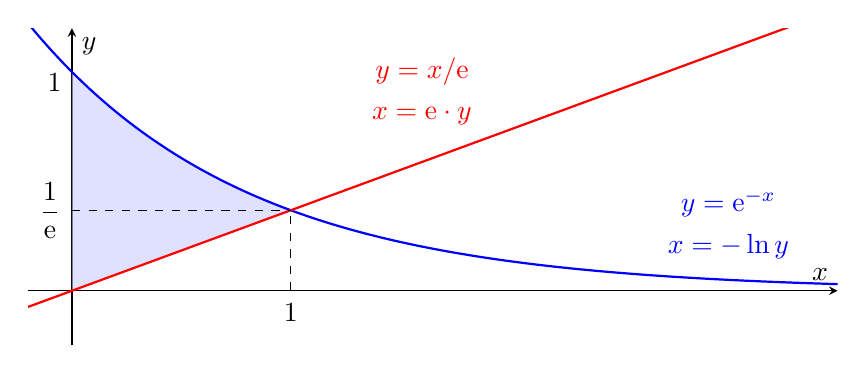
\begin{tikzpicture}
  \begin{axis}[
      axis lines=center,
      axis equal image,
      xlabel={$x$},
      ylabel={$y$},
      ytick=\empty, xtick=\empty,
      xmin=-0.2, xmax=3.5,
      ymin=-0.25, ymax=1.2,
      samples=250,
      clip=true,
      scale=1.5,
      domain=-0.5:4,
    ]

    \addplot [thick, blue, name path=A] {e^(-x)};
    \addplot [thick, red, name path=B] {x/e};
    \addplot [blue!20, fill opacity=0.6] fill between[of=A and B, soft clip={domain=0:1}];
    
    \node at (1,-0.1) {$1$};
    \node at (-0.1,0.367) {$\dfrac1{\mathrm e}$};
    \node at (-0.08,0.95) {$1$};

    \node[red] at (1.6,1) {$y=x/\mathrm{e}$};
    \node[red] at (1.6,0.8) {$x=\mathrm{e}\cdot y$};

    \node[blue] at (3,0.4) {$y=\mathrm{e}^{-x}$};
    \node[blue] at (3,0.2) {$x=-\ln y$};

    \draw[dashed] (0,0.367)--(1,0.367); \draw[dashed] (1,0)--(1,0.367);

  \end{axis}
\end{tikzpicture}
\end{center}

\[V=\int_D2\pi\cdot h(y)\cdot r(y)\,dy=\boxed{\int_0^{1/\mathrm e}2\pi\cdot y\cdot\left(\mathrm e\cdot y-0\right)\,dy+\int_{1/\mathrm e}^12\pi\cdot y\cdot\left(-\ln y-0\right)\,dy}\]

\newpage

\noindent (b)
\begin{center}
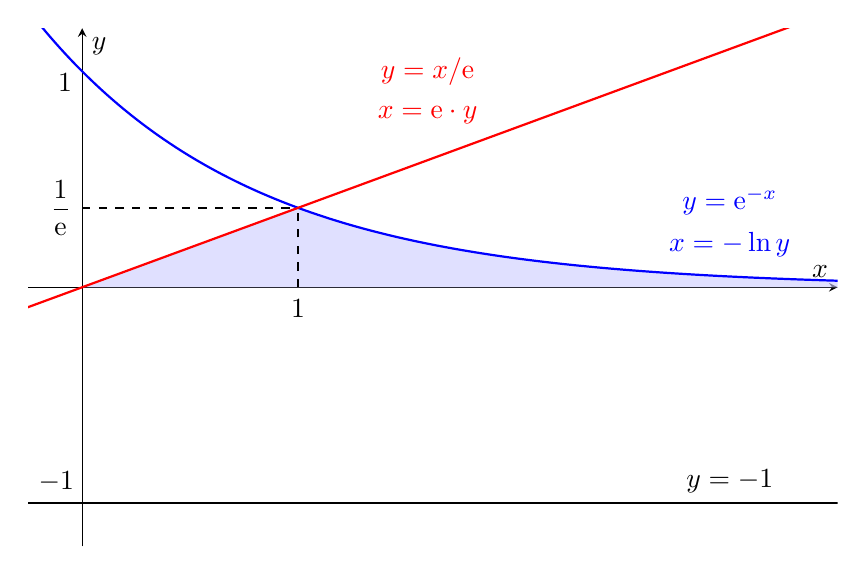
\begin{tikzpicture}
  \begin{axis}[
      axis lines=center,
      axis equal image,
      xlabel={$x$},
      ylabel={$y$},
      ytick=\empty, xtick=\empty,
      xmin=-0.25, xmax=3.5,
      ymin=-1.2, ymax=1.2,
      samples=250,
      clip=true,
      scale=1.5,
      domain=-0.5:4,
    ]

    \addplot [thick, blue, name path=A] {e^(-x)};
    \addplot [thick, red, name path=B] {x/e};
    \addplot [draw=none, name path=C] {0};
    \addplot [blue!20, fill opacity=0.6] fill between[of=B and C, soft clip={domain=0:1}];
    \addplot [blue!20, fill opacity=0.6] fill between[of=A and C, soft clip={domain=1:4}];

    \node at (1,-0.1) {$1$};
    \node at (-0.1,0.367) {$\dfrac1{\mathrm e}$};
    \node at (-0.08,0.95) {$1$};

    \node[red] at (1.6,1) {$y=x/\mathrm{e}$};
    \node[red] at (1.6,0.8) {$x=\mathrm{e}\cdot y$};

    \node[blue] at (3,0.4) {$y=\mathrm{e}^{-x}$};
    \node[blue] at (3,0.2) {$x=-\ln y$};

    \node at (-0.12,-0.9) {$-1$};
    \node at (3,-0.9) {$y=-1$};

    \draw[dashed] (0,0.367)--(1,0.367); \draw[dashed] (1,0)--(1,0.367); \draw[thick] (-1,-1)--(4,-1); 

  \end{axis}
\end{tikzpicture}
\end{center}
\[V=\int_D\pi\left[r_2^2(x)-r_1^2(x)\right]\,dx=\boxed{\int_0^1\left[\left(\frac x{\mathrm e}+1\right)^2-1^2\right]\,dx+\int_1^{\infty}\left[\left(\mathrm{e}^{-x}+1\right)^2-1^2\right]\,dx}\]

\hfill

\noindent (c)
\begin{equation}V=2\pi\left[\int_0^{1/\mathrm e}\mathrm{e}y^2\,dy-\int_{1/\mathrm e}^1y\ln y\,dy\right]\end{equation}

\hfill

\noindent Calculate the integral on the left in $(1)$.

\[\int_0^{1/\mathrm e}\mathrm{e}y^2\,dy=\frac{\mathrm{e}y^3}3\Bigg|_0^{1/\mathrm{e}}=\frac1{3\mathrm{e}^2}\]

\hfill

\noindent Calculate the integral on the right in $(1)$ by using the method of integration by parts.

\[\left.\begin{array}{c}
u=\ln x\implies du=\dfrac1x\,dx\\[1em]
dv=x\,dx\implies\displaystyle v=\frac{x^2}2
\end{array}\right\}\rightarrow\int_a^b u\,dv=uv\bigg|_a^b-\int_a^b v\,du\]

\begin{align*}\int_{1/\mathrm e}^1x\ln x\,dx&=\frac{x^2\ln x}2\Bigg|_{1/\mathrm{e}}^1-\int_{1/\mathrm{e}}^1\frac{x^2}2\cdot\frac1x\,dx=\frac{x^2\ln x}2-\frac{x^2}4\Bigg|_{1/\mathrm{e}}^1\\\\&=\left(0-\frac14\right)-\left(-\frac1{2\mathrm{e}^{2}}-\frac1{4\mathrm{e}^2}\right)=\frac3{4\mathrm{e}^2}-\frac14\end{align*}

\hfill

\noindent Therefore,

\[V=2\pi\left[\left(\frac1{3\mathrm{e}^2}\right)-\left(\frac3{4\mathrm{e}^2}-\frac14\right)\right]=\boxed{\pi\left(\frac12-\frac5{6\mathrm{e}^2}\right)}\]

\newpage

\noindent 3.

\hfill

\noindent (a) Apply the $n$th Term Test for divergence. The inverse trigonometric function $\arctan$ is continuous on $\mathbb{R}$. Therefore, we may take the limit inside the function.

\[\lim_{n\to\infty}\frac1{\arctan\left(n^2\right)}=\frac1{\arctan\left(\displaystyle\lim_{n\to\infty}n^2\right)}=\frac1{\dfrac\pi2}=\frac2\pi\neq1\]

\hfill

\noindent By the $n$th Term Test for divergence, the series $\displaystyle\sum_{n=1}^{\infty}\frac1{\arctan\left(n^2\right)}$ diverges.

\hfill

\hfill

\noindent (b) Recall the sine inequality $-\theta\leq\sin\theta\leq\theta$. Then for all $n\in\mathbb{R}$ except zero, we have $\displaystyle-\frac1{n^3}\leq\sin\left(\frac1{n^3}\right)\leq\frac1{n^3}$. The series $\displaystyle\sum_{n=1}^\infty\frac1{n^3}$ converges because it is a $p$-series with $p=3>1$. By the $p$-series Test, the series converges. The series $\displaystyle\sum_{n=1}^{\infty}\sin\left(\frac1{n^3}\right)$ also converges by the Direct Comparison Test because $\displaystyle\sin\left(\frac1{n^3}\right)<\frac1{n^3}$ for every $n\geq1$.

\hfill

\hfill

\noindent (c) Take $f(x)=x\mathrm{e}^{-x^2}$. $f$ is continuous because the product of a polynomial and an exponential expression is still continuous. $f$ is positive and decreasing for $x\geq1$. Verify the monotonicity of $f$ by taking the first derivative.

\[\frac{df}{dx}=1\cdot\mathrm{e}^{-x^2}+x\mathrm{e}^{-x^2}\cdot(-2x)=\mathrm{e}^{-x^2}\left(1-2x^2\right)\]

\[f'(x)<0\quad\text{for}\quad x>\frac{\sqrt2}2\implies f'(x)<0\quad\text{for}\quad x\geq1\]

\hfill

\noindent We may now apply the Integral Test. Take the limit for the improper integral.

\[\int_1^{\infty}x\mathrm{e}^{-x^2}\,dx=\lim_{R\to\infty}\int_1^Rx\mathrm{e}^{-x^2}\,dx=\lim_{R\to\infty}-\frac12\mathrm{e}^{-x^2}\Bigg|_1^R=\lim_{R\to\infty}-\frac12\left(\mathrm{e}^{-R^2}-\mathrm{e^{-1}}\right)=\frac1{2\mathrm{e}}\]

\hfill

\noindent The integral converges. Then the series $\displaystyle\sum_{n=1}^{\infty}n\mathrm{e}^{-n^2}$ also converges.

\hfill

\noindent 4.

\hfill

\noindent (a) Apply the Ratio Test for absolute convergence, and apply other tests at the endpoints.

\begin{align*}\lim_{n\to\infty}\left|\frac{2^{n+2}\cdot(x+1)^{n+1}}{(n+1)\cdot3^{n+1}}\cdot\frac{n\cdot3^n}{(x+1)^n\cdot2^{n+1}}\right|&=\lim_{n\to\infty}\left|\frac{2n\cdot(x+1)}{(n+1)\cdot3}\right|\\\\&=\frac{2|x+1|}3\cdot\lim_{n\to\infty}\left|\frac{n}{n+1}\right|=\frac{2|x+1|}3\end{align*}
\[\frac{2|x+1|}3<1\implies|x+1|<\frac32\]

\hfill

\noindent The radius of convergence is $\boxed{\dfrac32}$.

\hfill

\[|x+1|<\frac32\implies-\frac32<x+1<\frac32\implies-\frac52<x<\frac12\quad(\text{convergent})\]

\hfill

\noindent Investigate the convergence at the endpoints.

\[x=\frac12\implies\sum_{n=1}^{\infty}\frac{2^{n+1}\cdot\left(\dfrac32\right)^n}{n\cdot3^n}=\sum_{n=1}^{\infty}\frac2n=2\cdot\sum_{n=1}^{\infty}\frac1n\]

\hfill

\noindent This is a $p$-series with $p=1$, for which the series diverges by the $p$-series Test. Try the other endpoint.

\[x=-\frac52\implies\sum_{n=1}^{\infty}\frac{2^{n+1}\cdot\left(-\dfrac32\right)^n}{n\cdot3^n}=\sum_{n=1}^{\infty}\frac{2\cdot(-1)^n}n=2\cdot\sum_{n=1}^{\infty}\frac{(-1)^n}n\]

\hfill

\noindent This is an alternating series. The non-alternating part, which is $\frac1n$, is nonincreasing for $n\geq1$ and it is positive. The limit at infinity is $0$. By Leibniz's Alternating Series Test, the series converges.

\noindent The convergence set for the power series is $\boxed{\left[-\dfrac52,\dfrac12\right)}$.

\hfill

\noindent (b)
\begin{align*}f(x)&=\frac{x^{123}}{1+x^4}=x^{123}\cdot\frac1{1-\left(-x^4\right)}=x^{123}\cdot\sum_{n=0}^{\infty}\left(-x^4\right)=x^{123}\cdot\sum_{n=0}^{\infty}(-1)^n\cdot x^{4n}\\\\&=\boxed{\sum_{n=0}^{\infty}(-1)^n\cdot x^{123+4n}=x^{123}-x^{127}+x^{131}-x^{135}+...}\end{align*}

\newpage

\begin{center}
2024-2025 Final (09/01/2025) Solutions\\
(Last update: 21/08/2025 00:12)
\end{center}

\noindent 1.

\hfill

\noindent (a) Use the tangent half-angle substitution, which is also called the Weierstrass substitution. Let $\displaystyle t = \tan\left(\frac x2\right)$. Then

\[\sin x={\frac{2t}{1+t^{2}}},\quad\cos x={\frac{1-t^{2}}{1+t^{2}}},\quad dx={\frac2{1+t^{2}}}\,dt\]

\[\int\frac{dx}{2\cos x+3}=\int\frac1{2\left(\dfrac{1-t^2}{1+t^2}\right)+3}\cdot\frac2{1+t^2}\,dt=\int\frac2{5+t^2}\,dt=\frac25\int\frac1{\left(1+\left(\dfrac t{\sqrt5}\right)^2\right)}\,dt\]

\hfill

\noindent Let $u=\dfrac t{\sqrt5}$, then $\sqrt5\,du=dt$.

\begin{align*}\frac25\int\frac1{\left(1+\left(\dfrac t{\sqrt5}\right)^2\right)}\,dt&=\frac{2\sqrt5}5\int\frac1{1+u^2}\,du=\frac{2\sqrt5}5\arctan u+c=\frac{2\sqrt5}5\arctan\frac t{\sqrt5}+c\\&=\boxed{\frac{2\sqrt5}5\arctan\left(\frac1{\sqrt5}\cdot\tan\left(\frac x2\right)\right)+c,\quad c\in\mathbb{R}}\end{align*}

\hfill

\hfill

\noindent (b) Let $\displaystyle x=\sqrt5\sin u$ for $\displaystyle-\frac\pi2\leq u<\frac\pi2$, then $dx=\displaystyle\sqrt5\cos u\,du$.

\begin{align*}\mathrm{I}&=\int\frac{\sqrt{5-x^2}}{x}\,dx=\int\frac{\sqrt{5-5\sin^2u}}{\sqrt5\sin u}\cdot\sqrt5\cos u\,du\qquad\left[\sin^2u+\cos^2u=1\right]\\\\&=\sqrt5\int\sqrt{\cos^2u}\cot u\,du\qquad\left[\cos u>0\right]\\\\&=\sqrt5\int\cos u\cdot\cot u\,du=\sqrt5\int\frac{\cos^2u}{\sin u}\,du=\sqrt5\int\frac{1-\sin^2u}{\sin u}\,du\\\\&=\sqrt5\int\left(\csc u-\sin u\right)\,du=\sqrt5\left(-\ln\left|\cot u+\csc u\right|+\cos u\right)+c\end{align*}

\hfill

\noindent Recall that $\displaystyle x=\sqrt5\sin u$.

\[\sin u=\frac x{\sqrt5}\implies\sin^2u=\frac{x^2}5\implies\cos^2 u=\frac{5-x^2}5\implies\cos u=\frac{\sqrt{5-x^2}}{\sqrt5}\]

\[\cot u=\frac{\cos u}{\sin u}=\frac{\sqrt{5-x^2}}x,\qquad\csc u=\frac1{\sin u}=\frac{\sqrt5}x\]

\hfill

\noindent Therefore,
\[\mathrm{I}=\boxed{-\sqrt5\ln\left|\frac{\sqrt{5-x^2}}x+\frac{\sqrt5}x\right|+\sqrt{5-x^2}+c,\quad c\in\mathbb{R}}\]

\hfill

\noindent (c) Use partial fractions to compute the integral.

\begin{align*}\mathrm{I}&=\int\frac1{1-x^4}\,dx=\int\frac1{\left(1-x^2\right)\left(1+x^2\right)}\,dx=\int\frac1{(1-x)(1+x)\left(1+x^2\right)}\,dx\\\\&=\int\left(\frac A{1-x}+\frac B{1+x}+\frac{Cx+D}{1+x^2}\right)\,dx\end{align*}

\hfill

\[\begin{array}{c}
A(1+x)\left(1+x^2\right)+B(1-x)\left(1+x^2\right)+(Cx+D)(1+x)(1-x)=1\\
x^3(A-B-C)+x^2\left(A+B-D\right)+x\left(A-B+C\right)+A+B+D=1
\end{array}\]

\hfill

\noindent Equate the coefficients of like terms.

\[\left.\begin{array}{rc}
A-B-C=0&(1)\\
A+B-D=0&(2)\\
A-B+C=0&(3)\\
A+B+D=1&(4)
\end{array}\right\}\quad\begin{array}{c}
(1)\:\&\:(3)\rightarrow2A-2B=0\\
(2)\:\&\:(4)\rightarrow2A+2B=1\\[1em]
\therefore A=\dfrac14,\quad B=\dfrac14\\[1em]
(1)\rightarrow C=0,\quad (2)\rightarrow D=\dfrac12
\end{array}\]

\noindent Rewrite the integral.

\begin{align*}\mathrm{I}&=\int\left(\frac A{1-x}+\frac B{1+x}+\frac{Cx+D}{1+x^2}\right)\,dx=\int\left(\frac1{4(1-x)}+\frac1{4(1+x)}+\frac1{2\left(1+x^2\right)}\right)\,dx\\\\&=\boxed{-\frac14\ln|1-x|+\frac14\ln|1+x|+\frac12\arctan\left(x\right)+c,\: c\in\mathbb{R}}\end{align*}

\hfill

\noindent (d) Use the method of integration by parts.

\[\left.\begin{array}{cc}
u=\ln\left(1+x^2\right) \implies du=\dfrac{2x}{1+x^2}\,dx\\[1em]
dv=dx\implies v=x
\end{array}\right\}\rightarrow \int u\,dv=uv-\int v\,du\]
\begin{align*}\int\ln\left(1+x^2\right)\,dx&=x\ln\left(1+x^2\right)-\int\frac{2x^2}{1+x^2}\,dx=x\ln\left(1+x^2\right)-\int\frac{2x^2+2-2}{1+x^2}\,dx\\\\&=x\ln\left(1+x^2\right)-2\int dx+2\int\frac{\,dx}{1+x^2}\\\\&=\boxed{x\ln\left(1+x^2\right)-2x+2\arctan x+c,\quad c\in\mathbb{R}}\end{align*}

\newpage

\noindent 2.
\begin{center}
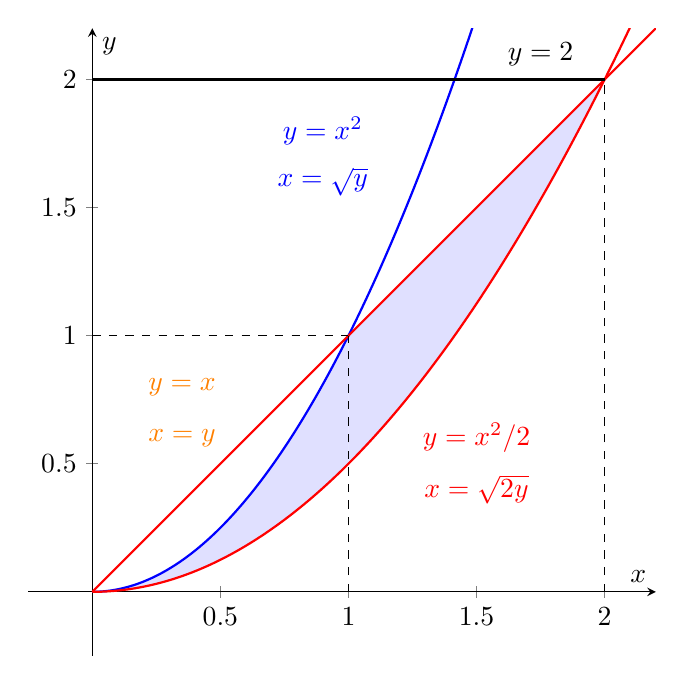
\begin{tikzpicture}
  \begin{axis}[
      axis lines=center,
      axis equal image,
      xlabel={$x$},
      ylabel={$y$},
      xmin=-0.25, xmax=2.2,
      ymin=-0.25, ymax=2.2,
      samples=250,
      clip=true,
      scale=1.4,
      domain=0:2.2,
    ]

    \addplot [thick, blue, name path=A] {x^2};
    \addplot [thick, red, name path=B] {x^2/2};
    \addplot [thick, red, name path=C] {x};
    \addplot [draw=none, name path=D] {0};
    \addplot [blue!20, fill opacity=0.6] fill between[of=A and B, soft clip={domain=0:1}];
    \addplot [blue!20, fill opacity=0.6] fill between[of=B and C, soft clip={domain=1:2}];
    
    \node[blue] at (0.9,1.8) {$y=x^2$};
    \node[red] at (1.5,0.6) {$y=x^2/2$};
    \node[orange] at (0.35,0.8) {$y=x$};
    \node at (1.75,2.1) {$y=2$};
    
    \node[blue] at (0.9,1.6) {$x=\sqrt y$};
    \node[red] at (1.5,0.4) {$x=\sqrt{2y}$};
    \node[orange] at (0.35,0.6) {$x=y$};
    
    \draw[dashed] (1,0)--(1,1); \draw[dashed] (0,1)--(1,1);
    \draw[dashed] (2,0)--(2,2); \draw[thick] (0,2)--(2,2);

  \end{axis}
\end{tikzpicture}
\end{center}

\noindent (a)
\begin{align*}A&=\int_0^1\left(x^2-\frac{x^2}2\right)\,dx+\int_1^2\left(x-\frac{x^2}2\right)\,dx=\left[\frac{x^3}3-\frac{x^3}6\right]_0^1+\left[\frac{x^2}2-\frac{x^3}6\right]_1^2\\\\&=\left[\left(\frac13-\frac16\right)-0\right]+\left[\left(2-\frac86\right)-\left(\frac12-\frac16\right)\right]=\boxed{\frac12}\end{align*}

\noindent (b)
\[V=\int_D\pi\left[r_2^2(y)-r_1^2(y)\right]\,dy=\boxed{\int_0^1\pi\left[\left(\sqrt{2y}\right)^2-\left(\sqrt y\right)^2\right]\,dy+\int_1^2\pi\left[\left(\sqrt{2y}\right)^2-y^2\right]\,dy}\]

\noindent (c)
\[V=\int_D2\pi\cdot h(y)\cdot r(y)\,dy=\boxed{\int_0^12\pi(2-y)\left(\sqrt{2y}-\sqrt{y}\right)dy+\int_1^22\pi(2-y)\left(\sqrt{2y}-y\right)dy}\]

\hfill

\noindent 3. Take $f(x)=x\mathrm{e}^{-x^2}$. $f$ is continuous because the product of a polynomial and an exponential expression is still continuous. $f$ is positive and decreasing for $x\geq1$. Verify the monotonicity of $f$ by taking the first derivative.

\[\frac{df}{dx}=1\cdot\mathrm{e}^{-x^2}+x\mathrm{e}^{-x^2}\cdot(-2x)=\mathrm{e}^{-x^2}\left(1-2x^2\right)\]

\[f'(x)<0\quad\text{for}\quad x>\frac{\sqrt2}2\implies f'(x)<0\quad\text{for}\quad x\geq1\]

\hfill

\noindent We may now apply the Integral Test. Take the limit for the improper integral.

\[\int_1^{\infty}x\mathrm{e}^{-x^2}\,dx=\lim_{R\to\infty}\int_1^Rx\mathrm{e}^{-x^2}\,dx=\lim_{R\to\infty}-\frac12\mathrm{e}^{-x^2}\Bigg|_1^R=\lim_{R\to\infty}-\frac12\left(\mathrm{e}^{-R^2}-\mathrm{e^{-1}}\right)=\frac1{2\mathrm{e}}\]

\hfill

\noindent The integral converges. Then the series $\displaystyle\sum_{n=1}^{\infty}n\mathrm{e}^{-n^2}$ also converges.

\hfill

\noindent 4. Apply the $n$th Term Test for the non-alternating part. Let $L$ be the value of the limit.

\[L=\lim_{n\to\infty}\left(\frac1n\right)^{1/n}\implies\ln(L)=\ln\left[\lim_{n\to\infty}\left(\frac1n\right)^{1/n}\right]\]

\hfill

\noindent We can also take the limit inside the function because $\ln$ is continuous on its domain.

\begin{align*}\ln(L)&=\lim_{n\to\infty}\ln\left[\left(\frac1n\right)^{1/n}\right]=\lim_{n\to\infty}\frac{\ln\left(\frac1n\right)}{n}\end{align*}

\hfill

\noindent To be able to use L'Hôpital's rule, take the corresponding function $f(x)=\dfrac{\ln\left(\frac1x\right)}x$.

\[\lim_{x\to\infty}\frac{\ln\left(\frac1x\right)}x\overset{\text{L'H.}}{=}\lim_{x\to\infty}\frac{x\cdot\left(-\frac1{x^2}\right)}1=\lim_{x\to\infty}-\frac1x=0\implies \ln(L)=0\implies L=1\]

\hfill

\noindent The limit $\displaystyle\lim_{n\to\infty}(-1)^{n+1}$ does not exist because of the oscillation. So, $\displaystyle\lim_{n\to\infty}(-1)^{n+1}\left(\frac1n\right)^{1/n}$ does not exist as well. Therefore, by the $n$th Term Test for divergence, the series $\displaystyle\sum_{n=1}^{\infty}(-1)^{n+1}\left(\frac1n\right)^{1/n}$ is divergent.

\hfill

\hfill

\noindent 5. The Maclaurin series of $f$ is given by $\sum_{k=0}^{\infty}\frac{f^{(k)}(0)}{k!}x^k$.

\hfill

\noindent Find $f(0),\:f'(0),\:f''(0),\:f'''(0)$ to look for the pattern.

\[f'(x)=\frac1{2\sqrt{\mathrm{e}^x}}\cdot\mathrm{e}^x=\frac12\sqrt{\mathrm{e}^x},\quad f''(x)=\frac1{4\sqrt{\mathrm{e}^x}}\cdot\mathrm{e}^x=\frac14\sqrt{\mathrm{e}^x},\quad f'''(x)=\frac1{8\sqrt{\mathrm{e}^x}}\cdot\mathrm{e}^x=\frac18\sqrt{\mathrm{e}^x}\]

\[f(0)=1,\quad f'(0)=\frac12,\quad f''(0)=\frac14,\quad f'''(0)=\frac18\]

\hfill

\noindent Therefore, $f^{(k)}(0)=\left(\dfrac12\right)^k$. Rewrite the summation formula.

\[\sum_{k=0}^{\infty}\frac{f^{(k)}(0)}{k!}x^k=\sum_{k=0}^{\infty}\frac{\left(\dfrac12\right)^k\cdot x^k}{k!}=\boxed{\sum_{k=0}^{\infty}\frac{x^k}{2^k\cdot k!}=1+\frac{x}2+\frac{x^2}8+\frac{x^3}{48}+...}\]

\hfill

\noindent Find the interval of convergence by applying the Ratio Test.

\[\lim_{k\to\infty}\left|\frac{x^{k+1}}{2^{k+1}\cdot\left(k+1\right)!}\cdot\frac{2^k\cdot k!}{x^k}\right|=\lim_{k\to\infty}\frac{x}{2k}=0<1\]

\hfill

\[\boxed{\text{The series is convergent on}\:\mathbb{R}.}\]

\newpage

\begin{center}
2024-2025 Makeup (31/01/2025) Solutions\\
(Last update: 17/08/2025 20:56)
\end{center}

\noindent 1.

\hfill

\noindent (a)
\[\int\frac{\sin^3x}{\sqrt{\cos x}}\,dx=\int\frac{\left(1-\cos^2x\right)\cdot\sin x}{\sqrt{\cos x}}\,dx\]

\hfill

\noindent Let $u=\cos x$, then $du=-\sin x\,dx$.

\begin{align*}\int\frac{\left(1-\cos^2x\right)\cdot\sin x}{\sqrt{\cos x}}\,dx&=\int-\frac{\left(1-u^2\right)}{\sqrt{u}}\,du=\int\left(u^{3/2}-\frac1{\sqrt u}\right)=\frac25u^{5/2}-2\sqrt u+c\\\\&=\boxed{\frac25\left(\cos x\right)^{5/2}-2\sqrt{\cos x}+c,\quad c\in\mathbb{R}}\end{align*}

\hfill

\noindent (b) Use the method of partial fraction decomposition.

\[\int\frac{dx}{x^3-4x^2+3x}=\int\frac{dx}{x(x-3)(x-1)}=\int\left(\frac Ax+\frac B{x-3}+\frac C{x-1}\right)\,dx\]

\[\begin{array}{rc}A(x-3)(x-1)+Bx(x-1)+Cx(x-3)&=1\\x^2(A+B+C)+x(-4A-B-3C)+3A&=1\\&\end{array}\]

\hfill

\noindent Equate the coefficients of like terms.

\[\left.\begin{array}{r}
x^2(A+B+C)=0\\
x(-4A-B-3C)=0\\
3A=1
\end{array}\right\}\rightarrow A=\frac13,\qquad\left.\begin{array}{r}
B+C=-\dfrac13\\[1em]
B+3C=-\dfrac43
\end{array}\right\}\rightarrow B=\frac16,\quad C=-\frac12\]

\hfill

\noindent Rewrite the integral.

\begin{align*}
\int\left(\frac Ax+\frac B{x-3}+\frac C{x-1}\right)\,dx&=\int\left(\frac1{3x}+\frac1{6(x-3)}-\frac1{2(x-1)}\right)\,dx\\\\&=\boxed{\frac13\ln|x|+\frac16\ln|x-3|-\frac12\ln|x-1|+c,\quad c\in\mathbb{R}}
\end{align*}

\hfill

\noindent (c) The limit is in the indeterminate form $0/0$. Apply L'Hôpital's rule to eliminate the indeterminate form.

\[\lim_{x\to\textstyle\frac\pi2}\frac{\displaystyle\int_{\pi/2}^x\ln(\sin t)\,dt}{\sin x-1}\overset{\text{L'H.}}{=}\lim_{x\to\textstyle\frac\pi2}\frac{\displaystyle\frac d{dx}\int_{\pi/2}^x\ln(\sin t)\,dt}{\cos x}\]

\hfill

\noindent By the Fundamental Theorem of Calculus, we may rewrite the limit as follows.

\begin{align*}\lim_{x\to\textstyle\frac\pi2}\frac{\displaystyle\frac d{dx}\int_{\pi/2}^x\ln(\sin t)\,dt}{\cos x}&=\lim_{x\to\textstyle\frac\pi2}\frac{\ln(\sin x)}{\cos x}\overset{\text{L'H.}}{=}\lim_{x\to\textstyle\frac\pi2}\frac{\frac1{\sin x}\cdot\cos x}{-\sin x}=\lim_{x\to\textstyle\frac\pi2}\frac{\cos x}{-\sin^2x}=-\frac{\cos\frac\pi2}{\sin^2\frac\pi2}\\\\&=\boxed0\end{align*}

\hfill

\noindent (d) Take the limit as this is an improper integral.

\begin{align*}\int_0^2\frac{dx}{(x-1)^{2/3}}&=\lim_{R\to1^-}\int_0^R\frac{dx}{(x-1)^{2/3}}+\lim_{P\to1^+}\int_P^2\frac{dx}{(x-1)^{2/3}}\\\\&=\lim_{R\to1^-}3(x-1)^{1/3}\Bigg|_0^R+\lim_{P\to1^+}3(x-1)^{1/3}\Bigg|_P^2\\\\&=3\lim_{R\to1^-}\left((R-1)^{1/3}-(-1)\right)+3\lim_{P\to1^+}\left(1-(P-1)^{1/3}\right)=\boxed6\end{align*}

\hfill

\noindent 2.

\hfill

\noindent (a)
\begin{center}
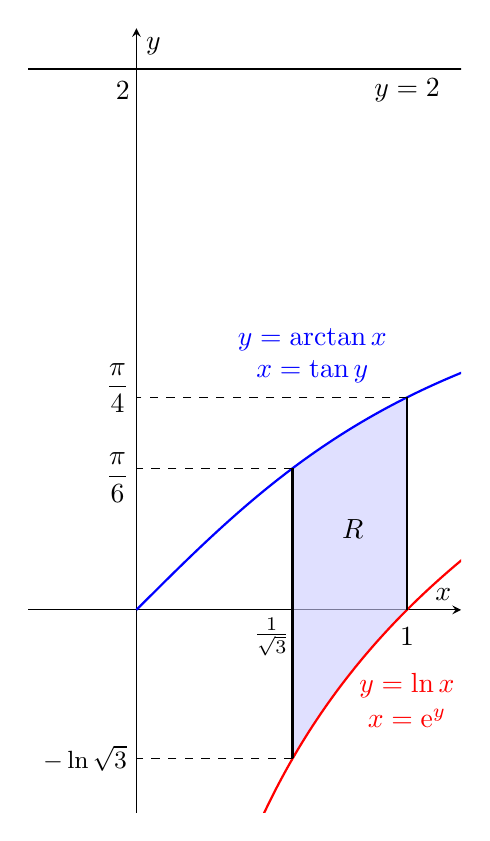
\begin{tikzpicture}
  \begin{axis}[
      axis lines=center,
      axis equal image,
      xlabel={$x$},
      ylabel={$y$},
      xmin=-0.4, xmax=1.2,
      ymin=-0.75, ymax=2.15,
      samples=200,
      scale=1.75,
      domain=0.577:1,
      xtick=\empty, ytick=\empty,
    ]

    \addplot [thick, blue, name path=A, domain=0:2] {rad(atan(x))};
    \addplot [thick, red, name path=B, domain=0.1:2] {ln(x)};
    \addplot [blue!20, fill opacity=0.6] fill between[of=A and B,soft clip={domain=0.577:1}];
    
    \draw[dashed] (-3,0) -- (-3,3); \draw[dashed] (-3,3) -- (-0.5,3);
    \draw[dashed] (2,0) -- (2,8); \draw[dashed] (0,8) -- (2,8);

    \node[blue] at (0.65,1) {$y=\arctan x$}; \node[blue] at (0.65,0.88) {$x=\tan y$};
    \node[red] at (1,-0.28) {$y=\ln x$}; \node[red] at (1,-0.4) {$x=\mathrm{e}^y$};

    \draw[thick] (0.577,-0.549)--(0.577,0.523); \draw[thick] (1,0)--(1,0.785);
    \draw[dashed] (1,0.785)--(0,0.785); \draw[dashed] (0.577, 0.523)--(0,0.523);
    \draw[dashed] (0.577,-0.549)--(0,-0.549);
    \draw[thick] (-1,2)--(2,2); 
    
    \node at (0.8,0.3) {$R$}; \node at (0.5,-0.1) {$\frac1{\sqrt3}$}; \node at (-0.07,0.49) {$\dfrac\pi6$}; \node at (-0.07,0.82) {$\dfrac\pi4$}; \node at (-0.19,-0.549) {\small $-\ln\sqrt3$}; \node at (1,-0.1) {$1$}; \node at (-0.05,1.92) {$2$}; \node at (1,1.92) {$y=2$};
\end{axis}
\end{tikzpicture}
\end{center}

\begin{equation}A=\int_{1/\sqrt3}^1\left(\arctan x-\ln x\right)\,dx=\int_{1/\sqrt3}^1\arctan x\,dx-\int_{1/\sqrt3}^1\ln x\,dx\end{equation}

\hfill

\noindent Calculate the first integral in $(1)$ by integration by parts.

\[\left.\begin{array}{c}
u=\arctan x\implies du=\dfrac1{x^2+1}\,dx\\[1em]
dv=dx\implies v=x
\end{array}\right\}\rightarrow \int u\,dv=uv-\int v\,du\]

\begin{align*}\int_{1/\sqrt3}^1\arctan x\,dx&=x\arctan x\bigg|_{1/\sqrt3}^1-\int_{1/\sqrt3}^1\frac{x}{x^2+1}\,dx=\left(x\arctan x-\frac12\ln\left|x^2+1\right|\right)\Bigg|_{1/\sqrt3}^1\\\\&=\left(\frac\pi4-\frac{\ln 2}2\right)-\left(\frac{\pi\sqrt3}{18}-\frac12\cdot\ln\left(\frac43\right)\right)=\frac{\pi\left(9-2\sqrt3\right)}{36}+\frac12\cdot\ln\frac23\end{align*}

\hfill

\noindent Calculate the second integral in $(1)$ by integration by parts.

\[\left.\begin{array}{c}
u=\ln x\implies du=\dfrac1x\,dx\\[1em]
dv=dx\implies v=x
\end{array}\right\}\rightarrow \int u\,dv=uv-\int v\,du\]

\begin{align*}\int_{1/\sqrt3}^1\ln x\,dx&=x\ln x\bigg|_{1/\sqrt3}^1-\int_{1/\sqrt3}^1\,dx=\left(x\ln x-x\right)\Bigg|_{1/\sqrt3}^1=\left(0-1\right)-\left(-\frac{\ln\sqrt3}{\sqrt3}-\frac1{\sqrt3}\right)\\\\&=\frac{\sqrt3\ln\sqrt3+\sqrt3-3}3\end{align*}

\hfill

\noindent The result is then

\[A=\boxed{\frac{\pi\left(9-2\sqrt3\right)}{36}+\frac12\cdot\ln\frac23-\frac{\sqrt3\ln\sqrt3+\sqrt3-3}3}\]

\hfill

\noindent (b)
\begin{align*}\boxed{\begin{array}{l}\displaystyle\int_{-\ln\sqrt3}^0\pi\left[\left(\mathrm{e}^y\right)^2-\left(\frac1{\sqrt3}\right)^2\right]\,dy+\int_0^{\pi/6}\pi\left[(1)^2-\left(\frac1{\sqrt3}\right)^2\right]\,dy\\\\\displaystyle+\int_{\pi/6}^{\pi/4}\pi\left[(1^2)-\left(\tan y\right)^2\right]\,dy\end{array}}\end{align*}

\hfill

\noindent (c)
\begin{align*}\boxed{\begin{array}{l}\displaystyle\int_{-\ln\sqrt3}^02\pi\left(2-y\right)\left(\mathrm{e}^y-\frac1{\sqrt3}\right)\,dy+\int_0^{\pi/6}2\pi\left(2-y\right)\left(1-\frac1{\sqrt3}\right)\,dy\\\\\displaystyle+\int_{\pi/6}^{\pi/4}2\pi\left(2-y\right)\left(1-\tan y\right)\,dy\end{array}}\end{align*}

\hfill

\noindent 3.

\hfill

\noindent (a)
\[\sum_{n=0}^{\infty}\frac{(-3)^{n+1}}{2^{3n}}=\sum_{n=0}^{\infty}\frac{-3\cdot(-3)^n}{8^n}=-3\sum_{n=0}^{\infty}\left(-\frac38\right)^n\]

\hfill

\noindent This is a geometric series where $r=-\dfrac38$. $|r|=\dfrac38<1$. Therefore, the series $\displaystyle\sum_{n=0}^{\infty}\frac{(-3)^{n+1}}{2^{3n}}$ converges.

\hfill

\noindent (b) Take $\displaystyle f(x)=\frac1{x(\ln x)^2}$. $f$ is positive and decreasing for $x\geq2$ because $x$ and $(\ln x)^2$ are positive and increasing for $x\geq2$. $x$ is a polynomial which is defined everywhere and $(\ln x)^2$ is continuous for $x\geq2$. Since we took into account every criterion, we may apply the Integral Test. Handle the improper integrals by taking the limit.

\[\int_2^{\infty}\frac{dx}{x(\ln x)^2}=\lim_{R\to\infty}\int_2^R\frac{dx}{x(\ln x)^2}=\lim_{R\to\infty}\left[-\frac1{\ln x}\right]_2^R=\lim_{R\to\infty}\left[-\frac1{\ln R}+\frac1{\ln2}\right]=\frac1{\ln 2}\]

\hfill

\noindent Since the integral converges, the series $\displaystyle\sum_{n=2}^\infty\frac1{n(\ln n)^2}$ also converges.

\hfill

\noindent 4. The Taylor series of $f$ at $c=1$ is as follows.

\[\sum_{k=0}^{\infty}\frac{f^{(k)}(1)}{k!}(x-1)^k\]

\hfill

\noindent Find $f(1),\:f'(1),\:f''(1),\:f'''(1)\:f^{(4)}(1)$ to look for the pattern.

\[f'(x)=\frac1{x},\quad f''(x)=-\frac1{x^2},\quad f'''(x)=\frac2{x^3}\quad f^{(4)}(x)=-\frac6{x^4} \]

\[f(1)=0,\quad f'(1)=1,\quad f''(1)=-1,\quad f'''(1)=2,\quad f^{(4)}(1)=-6\]

\hfill

\noindent This is an alternating sequence where the coefficient of each term is the factorial of the subsequent number starting from $0$ except for $k=0$, that is, the first term of the series. At $k=0$, the first term is $0$. So,

\[f^{k}(1)=\left\{\begin{array}{ll}(-1)^{k-1}\cdot (k-1)!,&\text{if}\: k>0\\0,& \text{if}\:k=0\end{array}\right.\]
\begin{align*}\sum_{k=0}^{\infty}\frac{f^{(k)}(1)}{k!}x^k&=0+\sum_{k=1}^{\infty}\frac{f^{(k)}(1)}{k!}(x-1)^k=\sum_{k=1}^{\infty}\frac{(-1)^{k-1}\cdot(k-1)!}{k\cdot(k-1)!}(x-1)^k\\\\&=\boxed{\sum_{k=1}^{\infty}\frac{(-1)^{k-1}\cdot(x-1)^k}{k}=(x-1)-\frac{(x-1)^2}2+\frac{(x-1)^3}3-\frac{(x-1)^4}4+...}\end{align*}

\hfill

\noindent Now, determine the interval of convergence. Apply the Ratio Test.

\begin{align*}\lim_{k\to\infty}\left|\frac{(-1)^k(x-1)^{k+1}}{k+1}\cdot\frac{k}{(-1)^{k-1}(x-1)^k}\right|&=\lim_{k\to\infty}\left|\frac{(x-1)\cdot k}{(k+1)\cdot(-1)}\right|=|x-1|\lim_{k\to\infty}\left|\frac k{k+1}\right|\\\\&=|x-1|\end{align*}

\[|x-1|<1\implies-1<x-1<1\implies0<x<2\quad(\text{convergent})\]

\hfill

\noindent Investigate the convergence at the endpoints.

\[x=0\rightarrow\sum_{k=1}^{\infty}\frac{(-1)^{k+1}\cdot(-1)^k}{k}=\sum_{k=1}^{\infty}\frac{(-1)^{2k}\cdot(-1)}{k}=-\sum_{k=1}^{\infty}\frac{1}{k}\]

\hfill

\noindent This is a $p$-series with $p=1$, for which the series diverges by the $p$-series Test. Try $x=2$.

\[x=2\rightarrow\sum_{k=1}^{\infty}\frac{(-1)^{k+1}}{k}\]

\hfill

\noindent This is an alternating series. The non-alternating part, which is $\frac1k$, is nonincreasing for $k\geq1$ and it is positive. The limit at infinity is $0$. By Leibniz's Alternating Series Test, the series converges.

\hfill

\noindent The convergence set for the power series is $\boxed{(0,2]}$.

\end{document}